\documentclass[11pt]{book}
\oddsidemargin 0in
\evensidemargin 0in
\marginparwidth 0in
\textheight 8in
\textwidth 6.5in
\topmargin 0in
\headheight 14pt
\usepackage{amssymb,amsmath,amsthm,fancyhdr,supertabular,longtable,hhline,mathtools}
\usepackage{colortbl}
\usepackage{import, multicol,boxedminipage}
\usepackage{chapterfolder}
\usepackage[metapost,truebbox]{mfpic}
\usepackage[pdflatex]{graphicx}
\usepackage{makeidx}
\usepackage[colorlinks, hyperindex, plainpages=false, linkcolor=blue, urlcolor=blue, pdfpagelabels]{hyperref}
\usepackage[all]{hypcap}
\usepackage{bm}
\definecolor{ResultColor}{gray}{0.9}
\theoremstyle{definition}  % this prevents the text in definitions, theorems, and corollaries from being italicized
\newtheorem{defn}{\bf Definition}[chapter]
\newtheorem{thm}{\bf Theorem}[chapter]
\newtheorem{cor}[thm]{\bf Corollary}
\newtheorem{eqn}{\bf Equation}[chapter]
\newtheorem{ex}{\bf Example}[section]
\newtheorem{fig}{\bf Figure}[chapter]
\setlength{\parindent}{0in}
\newcommand{\bbm}{\begin{boxedminipage}{6.41in}}
\newcommand{\ebm}{\end{boxedminipage}}
\usepackage{array}
\setlength{\extrarowheight}{2pt}
\allowdisplaybreaks[2]
\usepackage{cancel}
\usepackage{sectsty}
%\usepackage{appendix}
\usepackage{textcomp}
\usepackage{multirow}
\usepackage[nottoc]{tocbibind}

\DeclareSymbolFont{AMSb}{U}{msb}{m}{n}
\DeclareMathSymbol{\C}{\mathbin}{AMSb}{"43}
\DeclareMathSymbol{\N}{\mathbin}{AMSb}{"4E}
\DeclareMathSymbol{\I}{\mathbin}{AMSb}{"5A}
\DeclareMathSymbol{\Q}{\mathbin}{AMSb}{"51}
\DeclareMathSymbol{\R}{\mathbin}{AMSb}{"52}
\DeclareMathSymbol{\W}{\mathbin}{AMSb}{"57}

\allsectionsfont{\mdseries \scshape}
\makeatletter
\renewcommand\l@section{\@dottedtocline{1}{1.5em}{3em}}
\renewcommand\l@subsection{\@dottedtocline{2}{4.5em}{3.5em}}
\makeatother
\pagestyle{fancy}
\newcounter{HW}
\newcounter{HWindent}

\renewcommand{\textinterrobang}{$! \! \! ?$}

%Below is for Iowna Font
%\renewcommand*\sfdefault{iwona}
%\usepackage[math]{iwona}

%Below is for Helvetica (scaled): 
\usepackage[scaled=.92]{helvet}   
\renewcommand{\familydefault}{\sfdefault}  %makes the text of the book sans serif
\usepackage[helvet]{sfmath}  %makes the math in the book sans serif
\allsectionsfont{\sffamily}  %makes the chapter and section titles sans serif

\makeatletter
\newcases{mycases}{\quad}{%
  \hfil$\m@th\displaystyle{##}$}{$\m@th\displaystyle{##}$\hfil}{\lbrace}{.}
\makeatother

\begin{document}

\renewcommand{\textinterrobang}{$! \! \! ?$}

\chapter{\sc Polar Coordinates and Parametric Equations}

\documentclass{ximera}

\begin{document}
	\author{Stitz-Zeager}
	\xmtitle{TITLE}


\section{Polar Coordinates}

\documentclass{ximera}

\begin{document}
	\author{Stitz-Zeager}
	\xmtitle{TITLE}


\mfpicnumber{1}

\opengraphsfile{PolarCoordinates}

\setcounter{footnote}{0}

\label{PolarCoordinates}

In Section \ref{AppCartesianPlane}, we introduced the notion of assigning ordered pairs of real numbers called `coordinates'  to points in the plane.  Recall the Cartesian coordinate plane  is defined using two number lines -- one horizontal and one vertical -- which intersect at right angles at a point called the `origin'.   


\smallskip

As seen below on the left, to plot a point with Cartesian coordinates, say $P(-3,4)$, we start at the origin, travel horizontally to the left $3$ units, then up $4$ units. Alternatively, we could start at the origin, travel up $4$ units, then to the left $3$ units and arrive at the same location. 

\smallskip

For the most part, the `motions' of the Cartesian system (over and up) describe a rectangle, and most points can be thought of as the corner diagonally across the rectangle from the origin.\footnote{Excluding, of course, the points in which one or both coordinates are $0$.}  For this reason, the Cartesian coordinates of a point are often called  \index{rectangular coordinates ! also known as Cartesian coordinates} \index{coordinates ! rectangular} `rectangular' coordinates.  

\smallskip


\begin{center}
\begin{tabular}{cc}
\begin{mfpic}[15]{-5.5}{5.5}{-5.5}{5.5}
\drawcolor[gray]{0.7}
\polyline{(-5,-5), (-5,5)}
\polyline{(-4,-5), (-4,5)}
\polyline{(-3,-5), (-3,5)}
\polyline{(-2,-5), (-2,5)}
\polyline{(-1,-5), (-1,5)}
\polyline{(1,-5), (1,5)}
\polyline{(2,-5), (2,5)}
\polyline{(3,-5), (3,5)}
\polyline{(4,-5), (4,5)}
\polyline{(5,-5), (5,5)}
\polyline{(-5,-5), (5,-5)}
\polyline{(-5,-4), (5,-4)}
\polyline{(-5,-3), (5,-3)}
\polyline{(-5,-2), (5,-2)}
\polyline{(-5,-1), (5,-1)}
\polyline{(-5,1), (5,1)}
\polyline{(-5,2), (5,2)}
\polyline{(-5,3), (5,3)}
\polyline{(-5,4), (5,4)}
\polyline{(-5,5), (5,5)}
\drawcolor[rgb]{0.33,0.33,0.33}
\axes
\tlabel[cc](5.5,-0.5){\scriptsize $x$}
\tlabel[cc](0.5,5.5){\scriptsize $y$}
\xmarks{-4,-3,-2,-1,1,2,3,4}
\ymarks{-4,-3,-2,-1,1,2,3,4}
\point[3pt]{(0,0),(-3,4)}
\gclear \tlabelrect[cc](-4.5,4){\scriptsize $P(-3,4)$}
\tlpointsep{5pt}
\scriptsize
\axislabels {x}{{$-4 \hspace{7pt}$} -4, {$-3 \hspace{7pt} $} -3, {$-2\hspace{7pt} $} -2, {$-1 \hspace{7pt}$} -1, {$1$} 1, {$2$} 2, {$3$} 3, {$4$} 4}
\axislabels {y}{{$-4$} -4, {$-3$} -3, {$-2$} -2, {$-1$} -1, {$1$} 1, {$3$} 3, {$2$} 2}
\normalsize
\penwd{1.05pt}
\arrow \polyline{(0,0), (0,4)}
\arrow \polyline{(0,4), (-2.8,4)}
\arrow \polyline{(0,0), (-3,0)}
\arrow \polyline{(-3,0), (-3,3.8)}
\end{mfpic}

&

\begin{mfpic}[15]{-5.5}{5.5}{-5.5}{5.5}
\drawcolor{white}
\circle{(0,0), 5.5}
\drawcolor[gray]{0.7}
\circle{(0,0),1}
\circle{(0,0),2}
\circle{(0,0),3}
\circle{(0,0),4}
\circle{(0,0),5}
\polyline{(-4.33, -2.5), (4.33, 2.5)}
\polyline{(-4.33, 2.5), (4.33, -2.5)}
\polyline{(-2.5, -4.33), (2.5, 4.33)}
\polyline{(-2.5, 4.33), (2.5, -4.33)}
\polyline{(3.53, 3.53), (-3.53, -3.53)}
\polyline{(-3.53, 3.53), (3.53, -3.53)}
\polyline{(0, -5), (0, 5)}
\polyline{(-5, 0), (0, 0)}
\polyline{(4.83, 1.29), (-4.83, -1.29)}
\polyline{(-4.83, 1.29), (4.83, -1.29)}
\polyline{(1.29, 4.83), (-1.29, -4.83)}
\polyline{(-1.29, 4.83), (1.29, -4.83)}
\drawcolor[rgb]{0.33, 0.33, 0.33}
 \tlabel(2.5,-0.4){\scriptsize $r$}
\gclear \tlabelrect[cc](-1.77,1.77){\scriptsize $r$}
\gclear \tlabelrect[cc](1.25,2.16){\scriptsize $\theta$}
\gclear \tlabelrect[cc](0,-0.5){\scriptsize Pole}
 \tlabel[cc](6.5,0){\scriptsize Polar Axis}
\gclear \tlabelrect[cc](-4.5,4){\scriptsize $P(r,\theta)$}
\penwd{1.25pt}
\arrow \polyline{(0,0), (5,0)}
\arrow \polyline{(0,0), (-3,4)}
\arrow \parafcn{5, 120, 5}{2*dir(t)}
\point[3pt]{(0,0), (-3,4)}
\end{mfpic}


\end{tabular}
\end{center}




In this section, we introduce a new system for assigning coordinates to points in the plane --  \index{polar coordinates ! definition of} \index{coordinates ! polar}\textbf{polar coordinates} as diagrammed above on the right.  We start with an origin point, called the \index{polar coordinates ! pole} \textbf{pole}, and a ray called the \index{polar coordinates ! polar axis} \textbf{polar axis}. 

\smallskip

We locate a point $P$ using two coordinates, $(r,\theta)$, where $r$ represents a \textit{directed} distance from the pole\footnote{We will explain more about this momentarily.} and $\theta$ is a measure of counter-clockwise rotation from the polar axis.   

\smallskip

Roughly speaking,  the polar coordinates $(r,\theta)$ of a point measure `how far out' the point is from the pole (that's $r$), and `how far to rotate' from the polar axis, (that's $\theta$).

\smallskip


 For example, if we wished to plot the point $P$ with polar coordinates $\left(4, \frac{5\pi}{6}\right)$, we'd start at the pole, move out along the polar axis $4$ units, then rotate $\frac{5\pi}{6}$ radians counter-clockwise.


\begin{center}

\begin{tabular}{ccc}

\begin{mfpic}[15]{-5}{5}{-5}{5}
\xmarks{1,2,3,4}
\arrow \polyline{(0,0), (5,0)}
\point[3pt]{(0,0)}
\tlabel[cc](0,-0.5){\scriptsize Pole}
\tlabel[cc](2,0.5){\scriptsize $r=4$}
\penwd{1.05}
\arrow \polyline{(0,0), (4,0)}
\end{mfpic}

&

\begin{mfpic}[15]{-5}{5}{-5}{5}
\xmarks{1,2,3,4}
\arrow \polyline{(0,0), (5,0)}
\point[3pt]{(0,0)}
\tlabel[cc](0,-0.5){\scriptsize Pole}
\tlabel[cc](0,1.25){\scriptsize $\theta = \frac{5\pi}{6}$}
\arrow \parafcn{5, 145, 5}{0.75*dir(t)}
\point[3pt]{(-3.46,2)}
\penwd{1.05}
\arrow \polyline{(0,0), (-3.46,2)}
\end{mfpic}

&

\begin{mfpic}[15]{-5}{5}{-5}{5}
\xmarks{1,2,3,4}
\arrow \polyline{(0,0), (5,0)}
\point[3pt]{(0,0)}
\tlabel[cc](0,-0.5){\scriptsize Pole}
\point[3pt]{(-3.46,2)}
\tlabel[cc](-3.5,2.5){\scriptsize $P\left(4, \frac{5\pi}{6}\right)$}
\dotted \parafcn{5, 145, 5}{0.75*dir(t)}
\dotted \polyline{(0,0),(-3.46,2)}
\end{mfpic} \\

\end{tabular}

\end{center}

We may also visualize this process by thinking of the rotation first.\footnote{As with anything in Mathematics, the more ways you have to look at something, the better. The authors encourage the reader to take time to think about both approaches to plotting points given in polar coordinates.}  To plot $P\left(4,\frac{5\pi}{6}\right)$ this way,  we rotate  $\frac{5\pi}{6}$ counter-clockwise from the polar axis, then move outwards from the pole $4$ units.  Essentially we are locating a point on the terminal side of $\frac{5\pi}{6}$ which is $4$ units away from the pole.

\begin{center}

\begin{tabular}{ccc}

\begin{mfpic}[15]{-5}{5}{-5}{5}
\xmarks{1,2,3,4}
\arrow \polyline{(0,0), (5,0)}
\point[3pt]{(0,0)}
\tlabel[cc](0,-0.5){\scriptsize Pole}
\tlabel[cc](0,1.25){\scriptsize $\theta = \frac{5\pi}{6}$}
\arrow \parafcn{5, 145, 5}{0.75*dir(t)}
\dashed \rotatepath{(0,0),150} \polyline{(0,0),(5,0)}
\rotatepath{(0,0),150} \polyline{(1,-0.15),(1,0.15)}
\rotatepath{(0,0),150} \polyline{(2,-0.15),(2,0.15)}
\rotatepath{(0,0),150} \polyline{(3,-0.15),(3,0.15)}
\rotatepath{(0,0),150} \polyline{(4,-0.15),(4,0.15)}
\end{mfpic}

&

\begin{mfpic}[15]{-5}{5}{-5}{5}
\xmarks{1,2,3,4}
\arrow \polyline{(0,0), (5,0)}
\point[3pt]{(0,0)}
\tlabel[cc](0,-0.5){\scriptsize Pole}
\tlabel[cc](0,1.25){\scriptsize $\theta = \frac{5\pi}{6}$}
\arrow \parafcn{5, 145, 5}{0.75*dir(t)}
\point[3pt]{(-3.46,2)}
\dashed \rotatepath{(0,0),150} \polyline{(0,0),(5,0)}
\rotatepath{(0,0),150} \polyline{(1,-0.15),(1,0.15)}
\rotatepath{(0,0),150} \polyline{(2,-0.15),(2,0.15)}
\rotatepath{(0,0),150} \polyline{(3,-0.15),(3,0.15)}
\rotatepath{(0,0),150} \polyline{(4,-0.15),(4,0.15)}
\penwd{1.05}
\arrow \polyline{(0,0), (-3.46,2)}
\end{mfpic}

&

\begin{mfpic}[15]{-5}{5}{-5}{5}
\xmarks{1,2,3,4}
\arrow \polyline{(0,0), (5,0)}
\point[3pt]{(0,0)}
\tlabel[cc](0,-0.5){\scriptsize Pole}
\point[3pt]{(-3.46,2)}
\tlabel[cc](-3.5,2.5){\scriptsize $P\left(4, \frac{5\pi}{6}\right)$}
\dotted \parafcn{5, 145, 5}{0.75*dir(t)}
\dotted \polyline{(0,0),(-3.46,2) }
\end{mfpic} \\

\end{tabular}

\end{center}

If $r < 0$, we begin by moving in the opposite direction on the polar axis from the pole.  For example, to plot the point with polar coordinates $Q\left(-3.5, \frac{\pi}{4}\right)$ we have

\begin{center}

\begin{tabular}{ccc}

\begin{mfpic}[15]{-5}{5}{-5}{5}
\arrow \polyline{(0,0), (5,0)}
\dotted \polyline{(-4.5,0), (0,0)}
\xmarks{-4,-3,-2,-1,1,2,3,4}
\point[3pt]{(0,0)}
\tlabel[cc](0.3,-0.5){\scriptsize Pole}
\tlabel[cc](-1.75,0.5){\scriptsize $r=-3.5$}
\penwd{1.05}
\arrow \polyline{(0,0), (-3.5,0)}
\tlabel[cc](-2.5,-3){\scriptsize \phantom{$Q\left(-3.5, \frac{\pi}{4}\right)$}}
\end{mfpic}

&

\begin{mfpic}[15]{-5}{5}{-5}{5}
\arrow \polyline{(0,0), (5,0)}
\dotted \polyline{(0,0), (-4.5,0)}
\xmarks{-4,-3,-2,-1,1,2,3,4}
\point[3pt]{(0,0)}
\tlabel[cc](0.3,-0.5){\scriptsize Pole}
\tlabel[cc](-2.25,-0.75){\scriptsize $\theta = \frac{\pi}{4}$}
\arrow \parafcn{185, 220, 5}{1.25*dir(t)}
\point[3pt]{(-2.48,-2.48)}
\penwd{1.05}
\arrow \polyline{(0,0), (-2.48,-2.48)}
\tlabel[cc](-2.5,-3){\scriptsize \phantom{$Q\left(-3.5, \frac{\pi}{4}\right)$}}
\end{mfpic}

&

\begin{mfpic}[15]{-5}{5}{-5}{5}
\arrow \polyline{(0,0), (5,0)}
\dotted \polyline{(0,0), (-4.5,0)}
\xmarks{1,2,3,4}
\point[3pt]{(0,0)}
\tlabel[cc](0.3,-0.5){\scriptsize Pole}
\point[3pt]{(-2.48,-2.48)}
\tlabel[cc](-2.5,-3){\scriptsize $Q\left(-3.5, \frac{\pi}{4}\right)$}
\dotted  \parafcn{185, 220, 5}{1.25*dir(t)}
\dotted \polyline{(0,0),(-2.48,-2.48)}
\end{mfpic} \\

\end{tabular}

\end{center}

If we interpret the angle first, we rotate $\frac{\pi}{4}$ radians, then move back through the pole $3.5$ units.  Here we are locating a point $3.5$ units away from the pole on the terminal side of $\frac{5\pi}{4}$, not $\frac{\pi}{4}$.

\begin{center}

\begin{tabular}{ccc}

\begin{mfpic}[15]{-5}{5}{-5}{5}
\arrow \polyline{(0,0), (5,0)}
\xmarks{1,2,3,4}
\dashed \rotatepath{(0,0),45} \polyline{(0,0),(5,0)}
\rotatepath{(0,0),45} \polyline{(1,-0.15),(1,0.15)}
\rotatepath{(0,0),45} \polyline{(2,-0.15),(2,0.15)}
\rotatepath{(0,0),45} \polyline{(3,-0.15),(3,0.15)}
\rotatepath{(0,0),45} \polyline{(4,-0.15),(4,0.15)}
\point[3pt]{(0,0)}
\tlabel[cc](0.3,-0.5){\scriptsize Pole}
\tlabel[cc](2.15,0.5){\scriptsize $\theta = \frac{\pi}{4}$}
\arrow \parafcn{5, 40, 5}{1.25*dir(t)}
\tlabel[cc](-2.5,-3){\scriptsize \phantom{$Q\left(-3.5, \frac{\pi}{4}\right)$}}
\end{mfpic}

&

\begin{mfpic}[15]{-5}{5}{-5}{5}
\arrow \polyline{(0,0), (5,0)}
\xmarks{1,2,3,4}
\dashed \rotatepath{(0,0),45} \polyline{(0,0),(5,0)}
\rotatepath{(0,0),45} \polyline{(1,-0.15),(1,0.15)}
\rotatepath{(0,0),45} \polyline{(2,-0.15),(2,0.15)}
\rotatepath{(0,0),45} \polyline{(3,-0.15),(3,0.15)}
\rotatepath{(0,0),45} \polyline{(4,-0.15),(4,0.15)}
\dotted \rotatepath{(0,0),45} \polyline{(-4.75,0),(0,0)}
\rotatepath{(0,0),45} \polyline{(-1,-0.15),(-1,0.15)}
\rotatepath{(0,0),45} \polyline{(-2,-0.15),(-2,0.15)}
\rotatepath{(0,0),45} \polyline{(-3,-0.15),(-3,0.15)}
\rotatepath{(0,0),45} \polyline{(-4,-0.15),(-4,0.15)}
\point[3pt]{(0,0)}
\point[3pt]{(-2.48,-2.48)}
\tlabel[cc](0.3,-0.5){\scriptsize Pole}
\tlabel[cc](2.15,0.5){\scriptsize $\theta = \frac{\pi}{4}$}
\arrow \parafcn{5, 40, 5}{1.25*dir(t)}
\penwd{1.05}
\arrow \polyline{(0,0), (-2.48,-2.48)}
\tlabel[cc](-2.5,-3){\scriptsize \phantom{$Q\left(-3.5, \frac{\pi}{4}\right)$}}
\end{mfpic}

&

\begin{mfpic}[15]{-5}{5}{-5}{5}
\arrow \polyline{(0,0), (5,0)}
\dotted \rotatepath{(0,0),45} \polyline{(5,0),(0,0)}
\xmarks{1,2,3,4}
\point[3pt]{(0,0)}
\tlabel[cc](0.3,-0.5){\scriptsize Pole}
\point[3pt]{(-2.48,-2.48)}
\tlabel[cc](-2.5,-3){\scriptsize $Q\left(-3.5, \frac{\pi}{4}\right)$}
\dotted  \parafcn{5, 45, 5}{1.25*dir(t)}
\dotted \polyline{(0,0),(-2.48,-2.48)}\end{mfpic} \\

\end{tabular}

\end{center}

As you may have guessed, $\theta < 0$ means the rotation away from the polar axis is clockwise instead of counter-clockwise. Hence, to plot $R\left(3.5, -\frac{3\pi}{4}\right)$ we have the following.

\begin{center}

\begin{tabular}{ccc}

\begin{mfpic}[15]{-5}{5}{-5}{5}
\arrow \polyline{(0,0), (5,0)}
\xmarks{1,2,3,4}
\point[3pt]{(0,0)}
\tlabel[cc](0.3,-0.5){\scriptsize Pole}
\tlabel[cc](1.75,0.5){\scriptsize $r=3.5$}
\penwd{1.05}
\arrow \polyline{(0,0), (3.5,0)}
\tlabel[cc](-2.5,-3){\scriptsize \phantom{$R\left(3.5, -\frac{3\pi}{4}\right)$}}
\end{mfpic}

&

\begin{mfpic}[15]{-5}{5}{-5}{5}
\arrow \polyline{(0,0), (5,0)}
\xmarks{1,2,3,4}
\point[3pt]{(0,0)}
\tlabel[cc](0.3,-0.5){\scriptsize Pole}
\tlabel[cc](0.5,-1.75){\scriptsize $\theta = -\frac{3\pi}{4}$}
\arrow \parafcn{-5, -130, -5}{1.25*dir(t)}
\point[3pt]{(-2.48,-2.48)}
\penwd{1.05}
\arrow \polyline{(0,0), (-2.48,-2.48)}
\tlabel[cc](-2.5,-3){\scriptsize \phantom{$R\left(3.5, -\frac{3\pi}{4}\right)$}}
\end{mfpic}

&

\begin{mfpic}[15]{-5}{5}{-5}{5}
\arrow \polyline{(0,0), (5,0)}
\xmarks{1,2,3,4}
\point[3pt]{(0,0)}
\tlabel[cc](0.3,-0.5){\scriptsize Pole}
\point[3pt]{(-2.48,-2.48)}
\tlabel[cc](-2.5,-3){\scriptsize $R\left(3.5, -\frac{3\pi}{4}\right)$}
\dotted  \parafcn{-5, -130, -5}{1.25*dir(t)}
\dotted \polyline{(0,0),(-2.48,-2.48)}
\end{mfpic} \\

\end{tabular}

\end{center}

From an `angles first' approach, we rotate $-\frac{3\pi}{4}$ then move out $3.5$ units from the pole. We see that $R$ is the point on the terminal side of $\theta = -\frac{3\pi}{4}$ which is $3.5$ units from the pole.

\begin{center}


\begin{tabular}{ccc}

\begin{mfpic}[15]{-5}{5}{-5}{5}
\arrow \polyline{(0,0), (5,0)}
\xmarks{1,2,3,4}
\dashed \rotatepath{(0,0),45} \polyline{(-4.75,0),(0,0)}
\rotatepath{(0,0), 45} \polyline{(-1,-0.15),(-1,0.15)}
\rotatepath{(0,0), 45} \polyline{(-2,-0.15),(-2,0.15)}
\rotatepath{(0,0), 45} \polyline{(-3,-0.15),(-3,0.15)}
\rotatepath{(0,0),45} \polyline{(-4,-0.15),(-4,0.15)}
\point[3pt]{(0,0)}
\tlabel[cc](0.3,-0.5){\scriptsize Pole}
\tlabel[cc](0.5,-1.75){\scriptsize $\theta = -\frac{3\pi}{4}$}
\arrow \parafcn{-5, -130, -5}{1.25*dir(t)}
\tlabel[cc](-2.5,-3){\scriptsize \phantom{$R\left(3.5, -\frac{3\pi}{4}\right)$}}
\end{mfpic}

&

\begin{mfpic}[15]{-5}{5}{-5}{5}
\arrow \polyline{(0,0), (5,0)}
\xmarks{1,2,3,4}
\dashed \rotatepath{(0,0),45} \polyline{(-4.75,0),(0,0)}
\rotatepath{(0,0), 45} \polyline{(-1,-0.15),(-1,0.15)}
\rotatepath{(0,0), 45} \polyline{(-2,-0.15),(-2,0.15)}
\rotatepath{(0,0), 45} \polyline{(-3,-0.15),(-3,0.15)}
\rotatepath{(0,0),45} \polyline{(-4,-0.15),(-4,0.15)}
\point[3pt]{(0,0)}
\tlabel[cc](0.3,-0.5){\scriptsize Pole}
\tlabel[cc](0.5,-1.75){\scriptsize $\theta = -\frac{3\pi}{4}$}
\arrow \parafcn{-5, -130, -5}{1.25*dir(t)}
\point[3pt]{(-2.48,-2.48)}
\penwd{1.05}
\arrow \polyline{(0,0), (-2.48,-2.48)}
\tlabel[cc](-2.5,-3){\scriptsize \phantom{$R\left(3.5, -\frac{3\pi}{4}\right)$}}
\end{mfpic}

&

\begin{mfpic}[15]{-5}{5}{-5}{5}
\arrow \polyline{(0,0), (5,0)}
\xmarks{1,2,3,4}
\point[3pt]{(0,0)}
\tlabel[cc](0.3,-0.5){\scriptsize Pole}
\point[3pt]{(-2.48,-2.48)}
\tlabel[cc](-2.5,-3){\scriptsize $R\left(3.5, -\frac{3\pi}{4}\right)$}
\dotted  \parafcn{-5, -130, -5}{1.25*dir(t)}
\dotted \polyline{(0,0),(-2.48,-2.48)}
\end{mfpic} \\

\end{tabular}

\end{center}

The points $Q$ and $R$ above are, in fact, the same point despite the fact that their polar coordinate representations are different.  Unlike Cartesian coordinates where $(a,b)$ and $(c,d)$ represent the same point if and only if $a=c$ and $b=d$, a point can be represented by infinitely many polar coordinate pairs. 

\smallskip

We explore this notion more in the following example.

\begin{example} \label{plotpolarex} For each point in polar coordinates given below plot the point and then give two additional expressions for the point, one of which has $r > 0$ and the other with $r < 0$. 

\begin{multicols}{4}

\begin{enumerate}

\item  $P\left(2, 240^{\circ}\right)$

\item  $P\left(-4, \frac{7\pi}{6} \right)$

\item  $P\left(117, -\frac{5\pi}{2} \right)$

\item  $P\left(-3, -\frac{\pi}{4} \right)$

\end{enumerate}

\end{multicols}

{\bf Solution.}

\begin{enumerate}

\item  Whether we move $2$ units along the polar axis and then rotate $240^{\circ}$ or rotate $240^{\circ}$ then move out $2$ units from the pole, we plot  $P\left(2, 240^{\circ}\right)$  below. 

\begin{center}

\begin{tabular}{cc}

\begin{mfpic}[20]{-5}{5}{-5}{5}
\arrow \polyline{(0,0), (5,0)}
\xmarks{1,2,3,4}
\dashed \rotatepath{(0,0),240} \polyline{(0,0),(2.5,0)}
\rotatepath{(0,0),240} \polyline{(1,-0.15),(1,0.15)}
\rotatepath{(0,0),240} \polyline{(2,-0.15),(2,0.15)}
\point[3pt]{(0,0)}
\point[3pt]{(-1,-1.73)}
\tlabel[cc](0.5,-0.5){\scriptsize Pole}
\tlabel[cc](2.15,0.5){\scriptsize $\theta = 240^{\circ}$}
\arrow \parafcn{5, 235, 5}{0.75*dir(t)}
\penwd{1.05}
\arrow \polyline{(0,0), (-1,-1.73)}
\tlabel[cc](-1,-2.25){\scriptsize \phantom{$Q\left(2, 240^{\circ}\right)$}}
\end{mfpic}

&

\hspace{0.75in}

\begin{mfpic}[20]{-5}{5}{-5}{5}
\xmarks{1,2,3,4}
\arrow \polyline{(0,0), (5,0)}
\point[3pt]{(0,0)}
\tlabel[cc](0.5,-0.5){\scriptsize Pole}
\tlabel[cc](0,0.5){\scriptsize \phantom{Pole}}
\point[3pt]{(-1,-1.73)}
\tlabel[cc](-1,-2.25){\scriptsize $P\left(2, 240^{\circ}\right)$}
\dotted \parafcn{5, 235, 5}{0.75*dir(t)}
\dotted \polyline{(0,0),(-1,-1.73) }
\end{mfpic}

\\

\end{tabular}

\end{center}

We now set about finding alternate descriptions $(r,\theta)$ for the point $P$. Since $P$ is $2$ units from the pole, $r = \pm 2$.  Next, we choose angles $\theta$ for each of the $r$ values.  

\smallskip

The given representation for $P$ is $\left(2, 240^{\circ}\right)$ so the angle $\theta$ we choose for the  $r = 2$ case must be coterminal with $240^{\circ}$. (Can you see why?)  We choose $\theta = -120^{\circ}$, so one answer  is  $\left(2,-120^{\circ}\right)$. 

\smallskip

For the case  $r = -2$, we visualize our rotation starting $2$ units to the left of the pole.  From this position, we need only to rotate $\theta = 60^{\circ}$ to arrive at location coterminal with $240^{\circ}$.  Hence, our answer here is  $\left(-2,60^{\circ}\right)$.  We check our answers by plotting them.

\begin{center}

\begin{tabular}{cc}

\begin{mfpic}[20]{-5}{5}{-5}{5}
\xmarks{1,2,3,4}
\arrow \polyline{(0,0), (5,0)}
\point[3pt]{(0,0)}
\point[3pt]{(-1,-1.73)}
\tlabel[cc](-1,-2.5){\scriptsize $P\left(2, -120^{\circ}\right)$}
\dotted \parafcn{5, 235, 5}{0.75*dir(t)}
\arrow  \parafcn{-5, -115, -5}{0.75*dir(t)}
\dashed \rotatepath{(0,0),240} \polyline{(0,0),(2.5,0)}
\rotatepath{(0,0),240} \polyline{(1,-0.15),(1,0.15)}
\rotatepath{(0,0),240} \polyline{(2,-0.15),(2,0.15)}
\point[3pt]{(0,0)}
\point[3pt]{(-1,-1.73)}
\gclear \tlabelrect[cc](0.5,0.5){\scriptsize Pole}
\tlabel[cc](1.75,-0.5){\scriptsize $\theta = -120^{\circ}$}
\end{mfpic}
&
\hspace{0.5in}

\begin{mfpic}[20]{-5}{5}{-5}{5}
\xmarks{-2,-1,1,2,3,4}
\dotted \polyline{(0,0), (-5,0)}
\arrow \polyline{(0,0), (5,0)}
\point[3pt]{(0,0)}
\point[3pt]{(-1,-1.73)}
\tlabel[cc](-1,-2.5){\scriptsize $P\left(-2, 60^{\circ}\right)$}
\dotted \parafcn{5, 235, 5}{0.75*dir(t)}
\arrow  \parafcn{185, 235, 5}{1.25*dir(t)}
\dotted \rotatepath{(0,0),240} \polyline{(0,0),(2.5,0)}
\rotatepath{(0,0),240} \polyline{(1,-0.15),(1,0.15)}
\rotatepath{(0,0),240} \polyline{(2,-0.15),(2,0.15)}
\point[3pt]{(0,0)}
\point[3pt]{(-1,-1.73)}
\tlabel[cc](0.5,-0.5){\scriptsize Pole}
\tlabel[cc](-2,-0.75){\scriptsize $\theta = 60^{\circ}$}
\end{mfpic}

\\

\end{tabular}

\end{center}

\item  We plot $\left(-4,\frac{7\pi}{6}\right)$ by first moving $4$ units to the left of the pole and then rotating $\frac{7\pi}{6}$ radians.  Since $r = -4 < 0$, we find our point lies $4$ units from the pole on the terminal side of $\frac{\pi}{6}$.  

\begin{center}

\begin{tabular}{cc}

\begin{mfpic}[20]{-5}{5}{-5}{5}
\arrow \polyline{(0,0), (5,0)}
\dotted \polyline{(0,0), (-5,0)}
\xmarks{-4,-3,-2,-1,1,2,3,4}
\dotted \rotatepath{(0,0),30} \polyline{(0,0),(5,0)}
\rotatepath{(0,0),30} \polyline{(1,-0.15),(1,0.15)}
\rotatepath{(0,0),30} \polyline{(2,-0.15),(2,0.15)}
\rotatepath{(0,0),30} \polyline{(3,-0.15),(3,0.15)}
\rotatepath{(0,0),30} \polyline{(4,-0.15),(4,0.15)}
\point[3pt]{(0,0)}
\point[3pt]{(3.46,2)}
\tlabel[cc](-0.5,0.5){\scriptsize Pole}
\tlabel[cc](0,-1.5){\scriptsize $\theta = \frac{7\pi}{6}$}
\arrow \parafcn{185, 385, 5}{0.75*dir(t)}
\penwd{1.05}
\arrow \polyline{(0,0), (3.46,2)}
\end{mfpic}

&

\begin{mfpic}[20]{-5}{5}{-5}{5}
\arrow \polyline{(0,0), (5,0)}
\dotted \polyline{(0,0), (-5,0)}
\xmarks{1,2,3,4}
\point[3pt]{(0,0)}
\point[3pt]{(3.46,2)}
\tlabel[cc](-0.5,0.5){\scriptsize Pole}
\tlabel[cc](0,-1.5){\scriptsize \phantom{$\theta = \frac{7\pi}{6}$}}
\dotted \parafcn{185, 385, 5}{0.75*dir(t)}
\dotted \polyline{(0,0), (3.46,2)}
\tlabel(3.75,1.85){\scriptsize $P\left(-4,\frac{7\pi}{6}\right)$}
\end{mfpic}  \\

\end{tabular}

\end{center}

To find alternate descriptions for $P$, we note that the distance from $P$ to the pole is $4$ units, so any representation $(r,\theta)$ for $P$ must have $r = \pm 4$.  

\smallskip

As  noted above, $P$ lies on the terminal side of $\frac{\pi}{6}$, so this, coupled with $r=4$, gives us $\left(4, \frac{\pi}{6}\right)$ as one of our answers.  

\smallskip

To find a different representation for $P$ with $r = -4$, we may choose any angle coterminal with the angle $\theta =  \frac{7\pi}{6}$.  We pick $-\frac{5\pi}{6}$ and get $\left(-4, -\frac{5 \pi}{6}\right)$ as our second answer.

\begin{center}

\begin{tabular}{cc}

\begin{mfpic}[20]{-5}{5}{-5}{5}
\arrow \polyline{(0,0), (5,0)}
\dotted \polyline{(0,0), (-5,0)}
\xmarks{1,2,3,4}
\dashed \rotatepath{(0,0),30} \polyline{(0,0),(5,0)}
\rotatepath{(0,0),30} \polyline{(1,-0.15),(1,0.15)}
\rotatepath{(0,0),30} \polyline{(2,-0.15),(2,0.15)}
\rotatepath{(0,0),30} \polyline{(3,-0.15),(3,0.15)}
\rotatepath{(0,0),30} \polyline{(4,-0.15),(4,0.15)}
\point[3pt]{(0,0)}
\point[3pt]{(3.46,2)}
\tlabel(2,0.3){\scriptsize $\theta = \frac{\pi}{6}$}
\arrow \parafcn{2, 28, 5}{1.75*dir(t)}
\tlabel(3.5,1.5){\scriptsize $P\left(4,\frac{\pi}{6}\right)$}
\dotted \parafcn{185, 385, 5}{0.75*dir(t)}
\tlabel[cc](0,-1.25){\scriptsize Pole}
\end{mfpic}

&

\begin{mfpic}[20]{-5}{5}{-5}{5}
\arrow \polyline{(0,0), (5,0)}
\dotted \polyline{(0,0), (-5,0)}
\xmarks{-4,-3,-2,-1,1,2,3,4}
\dotted \rotatepath{(0,0),30} \polyline{(0,0),(5,0)}
\rotatepath{(0,0),30} \polyline{(1,-0.15),(1,0.15)}
\rotatepath{(0,0),30} \polyline{(2,-0.15),(2,0.15)}
\rotatepath{(0,0),30} \polyline{(3,-0.15),(3,0.15)}
\rotatepath{(0,0),30} \polyline{(4,-0.15),(4,0.15)}
\point[3pt]{(0,0)}
\point[3pt]{(3.46,2)}
\tlabel(-1,1){\scriptsize $\theta = -\frac{5\pi}{6}$}
\arrow \parafcn{175, 35, -5}{0.75*dir(t)}
\tlabel(3.5,1.5){\scriptsize $P\left(-4,-\frac{5\pi}{6}\right)$}
\dotted \parafcn{185, 385, 5}{0.75*dir(t)}
\tlabel[cc](0,-1.25){\scriptsize Pole}
\end{mfpic} \\

\end{tabular}

\end{center}

\item  To plot $P\left(117, -\frac{5\pi}{2} \right)$,  we move along the polar axis $117$ units from the pole and rotate \textit{clockwise} $\frac{5\pi}{2}$ radians as illustrated below.

\begin{center}

\begin{tabular}{cc}

\begin{mfpic}[15]{-5}{5}{-5}{5}
\arrow \polyline{(0,0), (5,0)}
\arrow \polyline{(0,0), (0,-5)}
\point[3pt]{(0,0)}
\point[3pt]{(0,-4.5)}
\tlabel[cc](0,0.5){\scriptsize Pole}
\tlabel[cc](2.5,-0.75){\scriptsize $\theta = - \frac{5\pi}{2}$}
\arrow \parafcn{0,445,5}{(t+200)*dir(0-t)/400}
\penwd{1.05}
\arrow \polyline{(0,0), (0,-4.5)}
\tlabel[cc](0,-5.5){\phantom{\scriptsize $P\left(117, -\frac{5\pi}{2}\right)$}}
\end{mfpic}

&
\hspace{1.55in}

\begin{mfpic}[15]{-5}{5}{-5}{5}
\arrow \polyline{(0,0), (5,0)}
\point[3pt]{(0,0)}
\point[3pt]{(0,-4.5)}
\tlabel[cc](0,0.5){\scriptsize Pole}
\dotted \parafcn{0,445,5}{(t+200)*dir(0-t)/400}
\dotted \polyline{(0,0), (0,-4.5)}
\tlabel[cc](0,-5.5){\scriptsize $P\left(117, -\frac{5\pi}{2}\right)$}
\end{mfpic} \\

\end{tabular}

\end{center}

Since $P$ is $117$ units from the pole, any representation $(r,\theta)$ for $P$ satisfies $r = \pm 117$.  

\smallskip

For the $r=117$ case, we can  take $\theta$ to be any angle coterminal with $-\frac{5\pi}{2}$.  In this case, we choose $\theta = \frac{3\pi}{2}$, and get $\left(117, \frac{3\pi}{2}\right)$ as one answer. 

\smallskip

For the $r = -117$ case,  we visualize moving left $117$ units from the pole and then rotating through an angle $\theta$ to reach $P$.  We find that $\theta = \frac{\pi}{2}$ works here, so our second answer is $\left(-117, \frac{\pi}{2}\right)$.


\begin{center}

\begin{tabular}{cc}

\begin{mfpic}[15]{-5}{5}{-5}{5}
\arrow \polyline{(0,0), (5,0)}
\point[3pt]{(0,0)}
\point[3pt]{(0,-4.5)}
\tlabel[cc](0,0.5){\scriptsize Pole}
\dotted \parafcn{0,445,5}{(t+200)*dir(0-t)/400}
\arrow \parafcn{5,265,5}{1.5 * dir(t)}
\dashed \polyline{(0,0), (0,-4.5)}
\tlabel[cc](-2.5,-1){\scriptsize $\theta = \frac{3\pi}{2}$}
\tlabel[cc](0,-5.5){\scriptsize $P\left(117, \frac{3\pi}{2}\right)$}
\end{mfpic}

&

\hspace{0.5in}

\begin{mfpic}[15]{-5}{5}{-5}{5}
\arrow \polyline{(0,0), (5,0)}
\dotted \polyline{(0,0), (-5,0)}
\point[3pt]{(0,0)}
\point[3pt]{(0,-4.5)}
\tlabel[cc](0,0.5){\scriptsize Pole}
\dotted \parafcn{0,445,5}{(t+200)*dir(0-t)/400}
\arrow \parafcn{185,265,5}{1.5*dir(t)}
\dotted \polyline{(0,0), (0,-4.5)}
\tlabel[cc](-2.5,-1){\scriptsize $\theta  = \frac{\pi}{2}$}
\tlabel[cc](0,-5.5){\scriptsize $P\left(-117, \frac{\pi}{2}\right)$}
\end{mfpic} \\

\end{tabular}

\end{center}

\item We move three units to the left of the pole and follow up with a clockwise rotation of $\frac{\pi}{4}$ radians to  plot $P\left(-3, -\frac{\pi}{4} \right)$.  We see that $P$ lies on the terminal side of $\frac{3\pi}{4}$.

\begin{center}

\begin{tabular}{cc}

\begin{mfpic}[20]{-5}{5}{-5}{5}
\arrow \polyline{(0,0), (5,0)}
\dotted \polyline{(0,0), (-5,0)}
\xmarks{-4,-3,-2,-1,1,2,3,4}
\dotted \rotatepath{(0,0),135} \polyline{(0,0),(5,0)}
\rotatepath{(0,0),135} \polyline{(1,-0.15),(1,0.15)}
\rotatepath{(0,0),135} \polyline{(2,-0.15),(2,0.15)}
\rotatepath{(0,0),135} \polyline{(3,-0.15),(3,0.15)}
\rotatepath{(0,0),135} \polyline{(4,-0.15),(4,0.15)}
\point[3pt]{(0,0)}
\point[3pt]{(-2.12,2.12)}
\tlabel[cc](0,-0.5){\scriptsize Pole}
\tlabel[cc](-2.75,0.5){\scriptsize $\theta = -\frac{\pi}{4}$}
\arrow \parafcn{175, 140, -5}{1.5*dir(t)}
\penwd{1.05}
\arrow \polyline{(0,0), (-2.12,2.12)}
\end{mfpic}

&

\begin{mfpic}[20]{-5}{5}{-5}{5}
\arrow \polyline{(0,0), (5,0)}
\dotted \polyline{(0,0), (-5,0)}
\xmarks{1,2,3,4}
\point[3pt]{(0,0)}
\point[3pt]{(-2.12,2.12)}
\tlabel[cc](0,-0.5){\scriptsize Pole}
\dotted \polyline{(0,0), (-2.12,2.12)}
\tlabel[cc](-2.12,2.5){\scriptsize $P\left(-3,-\frac{\pi}{4}\right)$}
\dotted \parafcn{175, 140, -5}{1.5*dir(t)}
\end{mfpic}  \\

\end{tabular}

\end{center}

Since $P$ lies on the terminal side of $\frac{3\pi}{4}$, one alternative representation for  $P$ is $\left(3, \frac{3\pi}{4}\right)$. 

\smallskip

 To find a different representation for $P$ with $r=-3$, we may choose any angle coterminal with $-\frac{\pi}{4}$.  We choose $\theta = \frac{7\pi}{4}$ for our final answer $\left(-3, \frac{7\pi}{4} \right)$.

\begin{center}

\begin{tabular}{cc}

\begin{mfpic}[20]{-5}{5}{-5}{5}
\arrow \polyline{(0,0), (5,0)}
\dotted \polyline{(0,0), (-5,0)}
\dashed\rotatepath{(0,0),135} \polyline{(0,0),(5,0)}
\rotatepath{(0,0),135} \polyline{(1,-0.15),(1,0.15)}
\rotatepath{(0,0),135} \polyline{(2,-0.15),(2,0.15)}
\rotatepath{(0,0),135} \polyline{(3,-0.15),(3,0.15)}
\rotatepath{(0,0),135} \polyline{(4,-0.15),(4,0.15)}
\xmarks{1,2,3,4}
\point[3pt]{(0,0)}
\point[3pt]{(-2.12,2.12)}
\tlabel[cc](0,-0.5){\scriptsize Pole}
\tlabel[cc](-1,2.25){\scriptsize $P\left(3,\frac{3\pi}{4}\right)$}
\dotted \parafcn{175, 140, -5}{1.5*dir(t)}
\arrow \parafcn{5, 130, 5}{0.75*dir(t)}
\tlabel[cc](1, 1){\scriptsize $\theta = \frac{3\pi}{4}$}
\drawcolor{white} \parafcn{240, 300, 5}{0.85*dir(t)}
\end{mfpic}

&

\begin{mfpic}[20]{-5}{5}{-5}{5}
\arrow \polyline{(0,0), (5,0)}
\dotted \polyline{(0,0), (-5,0)}
\dotted \rotatepath{(0,0),135} \polyline{(0,0),(5,0)}
\rotatepath{(0,0),135} \polyline{(1,-0.15),(1,0.15)}
\rotatepath{(0,0),135} \polyline{(2,-0.15),(2,0.15)}
\rotatepath{(0,0),135} \polyline{(3,-0.15),(3,0.15)}
\rotatepath{(0,0),135} \polyline{(4,-0.15),(4,0.15)}
\xmarks{-4,-3,-2,-1,1,2,3,4}
\point[3pt]{(0,0)}
\point[3pt]{(-2.12,2.12)}
\tlabel[cc](0,-0.5){\scriptsize Pole}
\tlabel[cc](-1,2.25){\scriptsize $P\left(-3,\frac{7\pi}{4}\right)$}
\dotted \parafcn{175, 140, -5}{1.5*dir(t)}
\arrow \parafcn{185, 490, 5}{0.85*dir(t)}
\tlabel[cc](1.5, 1){\scriptsize $\theta = \frac{7\pi}{4}$}
\end{mfpic}  \\

\end{tabular}

\end{center}

\end{enumerate}

\vspace{-.25in} \qed

\end{example}


In light of our work in Example \ref{plotpolarex}, it should come as no surprise that any given point expressed in polar coordinates has infinitely many other representations in polar coordinates.  

\smallskip

The following result characterizes when two sets of polar coordinates determine the same point in the plane.  It could be considered as a definition or a theorem, depending on your point of view.    We choose to state it as a property of the polar coordinate system.

\smallskip

%% \colorbox{ResultColor}{\bbm
\centerline{\textbf{Equivalent Representations of Points in Polar Coordinates}} \index{polar coordinates ! equivalent representations of}

\smallskip

Suppose $\left(r, \theta\right)$ and $\left(r', \theta'\right)$ are polar coordinates where $r \neq 0$, $r' \neq 0$ and the angles are measured in radians.  Then $\left(r, \theta\right)$ and $\left(r', \theta'\right)$  determine the same point $P$ if and only if one of the following is true:
 
 \begin{itemize}
 
 \item  $r' = r$ and $\theta' =  \theta + 2\pi k$ for some integer $k$
 
 \item  $r' = -r$ and $\theta' =  \theta + (2k + 1) \pi$ for some integer $k$
 
 \end{itemize}

All polar coordinates of the form $(0, \theta)$ represent the pole regardless of the value of $\theta$.

%% \ebm}

\smallskip

The key to understanding this result, and indeed the whole polar coordinate system, is to keep in mind that  $(r,\theta)$ means $(\text{directed distance from pole}, \text{angle of rotation})$. 

\smallskip

 If $r = 0$, then no matter how much rotation is performed, the point never leaves the pole.  Thus $(0, \theta)$ is the pole for all values of $\theta$.  
 
 \smallskip
 
 Now let's assume that neither $r$ nor $r'$ is zero.  If $\left(r, \theta\right)$ and $\left(r', \theta'\right)$ determine the same point $P$ then the (non-zero) distance from $P$ to the pole in each case must be the same.  Since this distance is controlled by the first coordinate, we have that either $r' = r$ or $r' = -r$.  
 
 \smallskip
 
 If $r' = r$, then when plotting $\left(r, \theta\right)$ and $\left(r', \theta'\right)$, the angles $ \theta$ and $ \theta'$ have the same initial side.  Hence, if $\left(r, \theta\right)$ and $\left(r', \theta'\right)$ determine the same point,   we must have that $\theta'$  is coterminal with  $\theta$.  We know that this means $\theta' = \theta + 2\pi k$ for some integer $k$, as required. 
 
 \smallskip
 
  If, on the other hand, $r' = -r$, then when plotting $\left(r, \theta\right)$ and $\left(r', \theta'\right)$, the initial side of $ \theta'$ is rotated $\pi$ radians away from the initial side of $\theta$.  In this case, $ \theta'$ must be coterminal with $\pi +  \theta$.  Hence, $ \theta' = \pi +  \theta + 2\pi k$ which we rewrite as $\theta' =  \theta + (2k+1)\pi$ for some integer $k$. 
  
  \smallskip
  
  Conversely, if $r' = r$ and $\theta' =  \theta + 2\pi k$ for some integer $k$, then  the points $P\left(r, \theta\right)$ and $P'\left(r', \theta'\right)$ lie the same (directed) distance from the pole on the terminal sides of coterminal angles, and hence are the same point.  
  
  \smallskip
  
Now suppose  $r' = -r$ and $\theta' = \theta + (2k + 1) \pi$ for some integer $k$.  To plot $P$, we first move a directed distance $r$ from the pole;  to plot $P'$, our first step is to move the same distance from the pole as $P$, but in the opposite direction.  At this intermediate stage, we have two points equidistant from the pole rotated exactly $\pi$ radians apart.  Since  $\theta' =  \theta + (2k + 1) \pi = \left(\theta + \pi\right) + 2\pi k $ for some integer $k$,  we see that $\theta'$ is coterminal to $\left(\theta + \pi\right)$ and it is this extra $\pi$ radians of rotation which aligns the points $P$ and $P'$.

\smallskip

Next, we marry the polar coordinate system with the Cartesian (rectangular) coordinate system.  To do so, we identify the pole and polar axis in the polar system to the origin and positive $x$-axis, respectively, in the rectangular system.  We get the following result.

\smallskip

%% \colorbox{ResultColor}{\bbm

\begin{theorem} \label{polarrectangularconversion} \textbf{Conversion Between Rectangular and Polar Coordinates:}  $~$

Suppose $P$ is represented in rectangular coordinates as $(x,y)$ and in polar coordinates as $(r,\theta)$.  Then

\begin{itemize}

\item $x = r \cos(\theta)$ and $y = r\sin(\theta)$ \index{polar coordinates ! conversion into rectangular}

\item $x^2+y^2 = r^2$ and $\tan(\theta) = \dfrac{y}{x}$ (provided $x \neq 0$) \index{rectangular coordinates ! conversion into polar}

\end{itemize}

\smallskip

\end{theorem}

%% \ebm}

\smallskip

In the case $r > 0$, Theorem \ref{polarrectangularconversion} is an immediate consequence of Theorems \ref{cosinesinecircle} and \ref{circularfunctionscircle}.

\smallskip

If $r < 0$, then we know an alternate representation for $(r,\theta)$ is $(-r, \theta + \pi)$.  Since in this case, $-r>0$, we know the theorem as stated is true for the representation $(-r, \theta + \pi)$ so we apply it here.

\smallskip

Applying Theorem \ref{polarrectangularconversion}  to $(-r,\theta+\pi)$ gives\footnote{Well,  Theorem \ref{polarrectangularconversion} along with the identities $\cos(\theta + \pi) = -\cos(\theta)$ and $\sin(\theta + \pi) = -\sin(\theta)$ \ldots}  $x = (-r) \cos(\theta + \pi) = (-r)(-\cos(\theta)) = r\cos(\theta)$  as well as  $y = (-r) \sin(\theta + \pi) = (-r)(-\sin(\theta)) = r\sin(\theta)$. 

\smallskip

Moreover, $x^2 + y^2 = (-r)^2 = r^2$, and $\frac{y}{x} = \tan(\theta + \pi) = \tan(\theta)$, so the theorem is true in this case, too.  

\smallskip

The remaining case is $r = 0$, in which case $(r,\theta) = (0,\theta)$ is the pole.  Since the pole is identified with the origin $(0,0)$ in rectangular coordinates, the theorem in this case amounts to checking `$0=0$.'  

\smallskip

Since we have argued that  Theorem \ref{polarrectangularconversion} is true in all cases, we put it to good use in the following example.

\smallskip


\begin{example}  \label{pointconversionex}   Convert each point in rectangular coordinates given below into polar coordinates with $r \geq 0$ and $0 \leq \theta < 2\pi$.  Use exact values if possible and round any approximate values to two decimal places.  Check your answer by converting them back to rectangular coordinates.

\begin{multicols}{4}

\begin{enumerate}

\item  $P\left(2,-2\sqrt{3}\right)$

\item  $Q(-3,-3)$

\item  $R(0,-3)$

\item  $S(-3,4)$

\end{enumerate}

\end{multicols}

{\bf Solution.}

Even though we are not explicitly told to do so, we can avoid many common mistakes by taking the time to plot the points before we do any calculations. 


\begin{enumerate}

\item  Plotting $P\left(2,-2\sqrt{3}\right)$, we find $P$ lies in Quadrant IV. With $x = 2$ and $y = -2\sqrt{3}$, we calculate $r^2 = x^2 + y^2 = (2)^2 + \left(-2\sqrt{3}\right)^2 = 4+12 = 16$ so $r = \pm 4$.  To satisfy $r \geq 0$, we choose $r = 4$.  

\smallskip

To find $\theta$, know $\tan(\theta) = \frac{y}{x} = \frac{-2\sqrt{3}}{2} = -\sqrt{3}$.  This tells us $\theta$ has a reference angle of $\frac{\pi}{3}$, and  since $P$ lies in Quadrant IV, we know $\theta$ is a Quadrant IV angle.   To satisfy the stipulation that $0 \leq \theta < 2\pi$, we choose $\theta = \frac{5\pi}{3}$.  Hence, our answer is  $\left(4, \frac{5\pi}{3}\right)$.  

\smallskip

To check, we convert  the polar representation $(r,\theta) = \left(4, \frac{5\pi}{3}\right)$ back to rectangular coordinates.   We find $x = r \cos(\theta) = 4 \cos\left(\frac{5\pi}{3}\right) = 4 \left(\frac{1}{2}\right) =  2$ and  $y = r \sin(\theta) = 4 \sin\left(\frac{5\pi}{3}\right) = 4 \left(-\frac{\sqrt{3}}{2}\right) = -2\sqrt{3}$.

\smallskip


\item  The point $Q(-3,-3)$ lies in Quadrant III.  Using $x = y = -3$, we get  $r^2 = (-3)^2 + (-3)^2 = 18$ so $r = \pm \sqrt{18} = \pm 3\sqrt{2}$.  To satisfy$r \geq 0$, we choose $r = 3 \sqrt{2}$.  

\smallskip

We find $\tan(\theta) = \frac{-3}{-3} = 1$, which means $\theta$ has a reference angle of $\frac{\pi}{4}$.  Since $Q$ lies in Quadrant III, we choose $\theta = \frac{5\pi}{4}$, to satisfy the requirement that $0 \leq \theta < 2\pi$.  Our final answer is  $\left(3\sqrt{2}, \frac{5\pi}{4}\right)$.  

\smallskip

Checking our answer, we find that $x = r\cos(\theta) = (3\sqrt{2}) \cos\left(\frac{5\pi}{4}\right) = (3\sqrt{2})\left(-\frac{\sqrt{2}}{2}\right) = -3$ and compute  $y = r\sin(\theta) = (3\sqrt{2}) \sin\left(\frac{5\pi}{4}\right) = (3\sqrt{2})\left(-\frac{\sqrt{2}}{2}\right) = -3$, so we are done.


\begin{center}

\begin{tabular}{cc}

\begin{mfpic}[15]{-5}{5}{-5}{5}
\axes
\dashed\rotatepath{(0,0),300} \polyline{(0,0),(5,0)}
\rotatepath{(0,0), 300} \polyline{(1,-0.15),(1,0.15)}
\rotatepath{(0,0), 300} \polyline{(2,-0.15),(2,0.15)}
\rotatepath{(0,0),300} \polyline{(3,-0.15),(3,0.15)}
\rotatepath{(0,0),300} \polyline{(4,-0.15),(4,0.15)}
\xmarks{-4,-3,-2,-1,1,2,3,4}
\ymarks{-4,-3,-2,-1,1,2,3,4}
\tlabel[cc](5,-0.25){\scriptsize $x$}
\tlabel[cc](0.25,5){\scriptsize $y$}
\tlabel[cc](2.5,-3.5){\scriptsize $P$}
\point[3pt]{(0,0)}
\point[3pt]{(2,-3.46)}
\arrow \parafcn{5, 295, 5}{0.75*dir(t)}
\tlabel[cc](1.5, 1){\scriptsize $\theta = \frac{5\pi}{3}$}
\end{mfpic}

&

\begin{mfpic}[15]{-5}{5}{-5}{5}
\axes
\dashed\rotatepath{(0,0), 225} \polyline{(0,0),(5,0)}
\rotatepath{(0,0), 225} \polyline{(1,-0.15),(1,0.15)}
\rotatepath{(0,0), 225} \polyline{(2,-0.15),(2,0.15)}
\rotatepath{(0,0), 225} \polyline{(3,-0.15),(3,0.15)}
\rotatepath{(0,0),225} \polyline{(4,-0.15),(4,0.15)}
\tlabel[cc](5,-0.25){\scriptsize $x$}
\tlabel[cc](0.25,5){\scriptsize $y$}
\xmarks{-4,-3,-2,-1,1,2,3,4}
\ymarks{-4,-3,-2,-1,1,2,3,4}
\point[3pt]{(0,0)}
\point[3pt]{(-3,-3)}
\tlabel[cc](-3.5,-3){\scriptsize $Q$}
\arrow \parafcn{5, 220, 5}{0.75*dir(t)}
\tlabel[cc](1.5, 1){\scriptsize $\theta = \frac{5\pi}{4}$}
\end{mfpic}  \\

$P$ has rectangular coordinates $(2,-2\sqrt{3})$ & $Q$ has rectangular coordinates $(-3,-3)$ \\
$P$ has polar coordinates $\left(4,\frac{5\pi}{3}\right)$ & $Q$ has polar coordinates $\left(3\sqrt{2}, \frac{5\pi}{4}\right)$  \\

\end{tabular}

\end{center}

\item The point $R(0,-3)$ lies along the negative $y$-axis.  While we could go through the usual computations\footnote{Since $x=0$, we would have to determine $\theta$ geometrically.} to find the polar form of $R$, in this case it is much more efficient to find the polar coordinates of $R$ using the definition.

\smallskip

 Since the pole is identified with the origin, we see the point $R$ is $3$ units from the pole.  Hence in the polar representation $(r, \theta)$ of $R$ we know $r = \pm 3$.  To satisfy $r \geq 0$, we choose $r = 3$.  
 
 \smallskip
 
 Concerning $\theta$, we once again find more or less `by inspection' that $\theta = \frac{3\pi}{2}$ satisfies $0 \leq \theta < 2\pi$ with its terminal side along the negative $y$-axis.  Hence, our answer is $\left(3, \frac{3\pi}{2}\right)$.  
 
 \smallskip
 
 To check, we note $x = r \cos(\theta) = 3 \cos\left( \frac{3\pi}{2}\right) = (3)(0) = 0$ and $y = r \sin(\theta) = 3 \sin\left( \frac{3\pi}{2}\right) = 3(-1) = -3$.

\item  The point $S(-3,4)$ lies in Quadrant II.  With $x = -3$ and $y = 4$, we get $r^2 = (-3)^2 + (4)^2 = 25$ so $r = \pm 5$.  As usual, we choose $r = 5 \geq 0$ and proceed to determine $\theta$.  

\smallskip

We have $\tan(\theta) = \frac{y}{x} = \frac{4}{-3} = -\frac{4}{3}$, and since this isn't the tangent of one the common angles, we resort to using the arctangent function. Since $\theta$ lies in Quadrant II and must satisfy $0 \leq \theta < 2\pi$, we choose $\theta = \pi - \arctan\left(\frac{4}{3}\right)$ radians.  Hence, our answer is $(r,\theta) = \left(5, \pi - \arctan\left(\frac{4}{3}\right)\right) \approx (5,2.21)$.  

\smallskip

To check our answers requires a bit of tenacity since we need to simplify expressions of the form:  $\cos\left(\pi - \arctan\left(\frac{4}{3}\right)\right)$ and $\sin\left(\pi - \arctan\left(\frac{4}{3}\right)\right)$.  These are good review exercises (see Section \ref{TheInverseTrigonometricFunctions}) and are hence left to the reader.  We find  $\cos\left(\pi - \arctan\left(\frac{4}{3}\right)\right) = -\frac{3}{5}$ and $\sin\left(\pi - \arctan\left(\frac{4}{3}\right)\right) = \frac{4}{5}$ , so that $x = r \cos(\theta) = (5)\left(-\frac{3}{5}\right) = -3$ and $y = r \sin(\theta) = (5) \left(\frac{4}{5}\right) = 4$ which confirms our answer.

\end{enumerate}

\begin{center}

\begin{tabular}{cc}

\begin{mfpic}[15]{-5}{5}{-5}{5}
\axes
\xmarks{-4,-3,-2,-1,1,2,3,4}
\ymarks{-4,-3,-2,-1,1,2,3,4}
\tlabel[cc](5,-0.25){\scriptsize $x$}
\tlabel[cc](0.25,5){\scriptsize $y$}
\point[3pt]{(0,0)}
\point[3pt]{(0,-3)}
\tlabel[cc](0.5,-3){\scriptsize $R$}
\arrow \parafcn{5, 265, 5}{0.75*dir(t)}
\tlabel[cc](1.5, 1){\scriptsize $\theta = \frac{3\pi}{2}$}
\end{mfpic}

&

\begin{mfpic}[15]{-5}{5}{-5}{5}
\axes
\dashed\rotatepath{(0,0), 127} \polyline{(0,0),(5,0)}
\rotatepath{(0,0), 127} \polyline{(1,-0.15),(1,0.15)}
\rotatepath{(0,0), 127} \polyline{(2,-0.15),(2,0.15)}
\rotatepath{(0,0), 127} \polyline{(3,-0.15),(3,0.15)}
\rotatepath{(0,0), 127} \polyline{(4,-0.15),(4,0.15)}
\tlabel[cc](5,-0.25){\scriptsize $x$}
\tlabel[cc](0.25,5){\scriptsize $y$}
\xmarks{-4,-3,-2,-1,1,2,3,4}
\ymarks{-4,-3,-2,-1,1,2,3,4}
\point[3pt]{(0,0)}
\point[3pt]{(-3,4)}
\tlabel[cc](-3.5,4){\scriptsize $S$}
\arrow \parafcn{5, 120, 5}{0.75*dir(t)}
\tlabel[cc](3, 1){\scriptsize $\theta =\pi - \arctan\left(\frac{4}{3}\right)$}
\end{mfpic}  \\

$R$ has rectangular coordinates $(0,-3)$ & $S$ has rectangular coordinates $(-3,4)$ \\
$R$ has polar coordinates $\left(3,\frac{3\pi}{2}\right)$ & $S$ has polar coordinates $\left(5, \pi - \arctan\left(\frac{4}{3}\right)\right)$  \\

\end{tabular}

\end{center}

\vspace{-.25in} \qed

\end{example}

\medskip

Now that we've had practice converting representations of \textit{points} between the rectangular and polar coordinate systems, we now set about converting \textit{equations} from one system to another.  

\smallskip

Just as we've used equations in $x$ and $y$ to represent relations in rectangular coordinates (see Section \ref{Relations}), equations in the variables $r$ and $\theta$ represent relations in polar coordinates.  We convert equations between the two systems using Theorem \ref{polarrectangularconversion} as the next example illustrates.

\medskip

\begin{example} \label{eqnconversionex} $~$

\begin{enumerate}

\item \label{recteqntopolar} Convert each equation in rectangular coordinates into an equation in polar coordinates.

\begin{multicols}{3}

\begin{enumerate}

\item  \label{ris6costheta} $(x-3)^2 + y^2 = 9$

\item  \label{yisnegx} $y = -x$

\item  \label{yisxsquared} $y = x^2$

\end{enumerate}

\end{multicols}

\enlargethispage{.5in}

\item \label{polareqntorect} Convert each equation in polar coordinates into an equation in rectangular coordinates.
 
\begin{multicols}{3}

\begin{enumerate}

\item  \label{risneg3} $r = -3$

\item  $\theta = \frac{4\pi}{3}$

\item \label{cardioidtorect} $r = 1 - \cos(\theta)$

\end{enumerate}

\end{multicols}

\end{enumerate} 

{\bf Solution.}



\begin{enumerate}

\item  One strategy to convert an equation from rectangular to polar coordinates is to replace every occurrence of $x$ with $r\cos(\theta)$ and every occurrence of $y$ with $r\sin(\theta)$ and use identities to simplify.  This is the technique we employ below.

\begin{enumerate}

\item We start by substituting  $x = r\cos(\theta)$ and $y = \sin(\theta)$ into $(x-3)^2 + y^2 = 9$ and simplifying.  With no real direction in which to proceed, we follow our mathematical instincts.\footnote{Experience is the mother of all instinct, and necessity is the mother of invention.  Study this example and see what techniques are employed, then try your best to get your answers in the homework to match Jeff's.}
\[ \begin{array}{rclr}

(r\cos(\theta) - 3)^2+ (r\sin(\theta))^2 & = & 9& \\[3pt]
r^2\cos^2(\theta) - 6 r\cos(\theta) + 9 + r^2 \sin^{2}(\theta) & = &  9 \\[3pt]
r^2\left(\cos^2(\theta) + \sin^{2}(\theta)\right) - 6 r\cos(\theta) & = & 0 & \text{Subtract $9$ from both sides.}\\[3pt]
r^2 - 6 r\cos(\theta) & = & 0 & \text{Since $\cos^2(\theta) + \sin^2(\theta) = 1$} \\[3pt]
r(r - 6 \cos(\theta)) & = & 0 &  \text{Factor.} \\ \end{array} \]

We get $r = 0$ or $r = 6\cos(\theta)$.  From Section \ref{Circles} we know the equation $(x-3)^2 + y^2 = 9$ describes a circle, and since $r=0$ describes just a point (namely the pole/origin), we choose $r = 6\cos(\theta)$ for our final answer.\footnote{Note when we substitute $\theta = \frac{\pi}{2}$ into the equation $r = 6\cos(\theta)$,  we recover the point $r = 0$.}

\item  Substituting $x = r\cos(\theta)$ and $y = r\sin(\theta)$ into $y=-x$ gives $r\sin(\theta)= -r\cos(\theta)$.  Rearranging, we get  $r\cos(\theta) + r\sin(\theta) = 0$ or $r(\cos(\theta) + \sin(\theta)) = 0$.  This gives $r=0$ or $\cos(\theta) + \sin(\theta) = 0$.  Solving the latter equation for $\theta$, we get $\theta = -\frac{\pi}{4} + \pi k$ for integers $k$. 

\smallskip

As we did in the previous example, we take a step back and think geometrically. We know $y=-x$ describes a line through the origin.  As before, $r=0$ describes the origin, but nothing else.  Consider the equation $\theta = -\frac{\pi}{4}$.  In this equation, the variable $r$ is free,\footnote{See Section \ref{LinSystems}.} meaning it can assume any and all values including $r=0$. 

\smallskip

If we imagine plotting points $(r, -\frac{\pi}{4})$  for all conceivable values of $r$ (positive, negative and zero), we are essentially drawing the line containing the terminal side of $\theta = -\frac{\pi}{4}$ which is none other than $y = -x$.  Hence, we can take as our final answer   $\theta = -\frac{\pi}{4}$ here.\footnote{We could take it to be \textit{any} of $\theta = -\frac{\pi}{4} + \pi k$ for integers $k$.} 

\item  Substituting $x = r\cos(\theta)$ and $y = r\sin(\theta)$ into $y = x^2$ gives $r\sin(\theta) = (r\cos(\theta))^2$, or $r^2\cos^2(\theta) - r\sin(\theta) = 0$.  Factoring, we get $r(r\cos^2(\theta) - \sin(\theta)) = 0$ so either $r=0$ or $r\cos^2(\theta) = \sin(\theta)$. 

\smallskip

We can solve  $r\cos^2(\theta) = \sin(\theta)$ for $r$ by dividing both sides of the equation by $\cos^{2}(\theta)$, but as a general rule, we never divide through by a quantity that may be $0$.  

\smallskip

In this particular case, we are safe since if $\cos^{2}(\theta) = 0$, then $\cos(\theta) = 0$,  and for the equation $r\cos^2(\theta) = \sin(\theta)$  to hold, then $\sin(\theta)$ would also have to be $0$.  Since there are no angles with both $\cos(\theta) = 0$ and $\sin(\theta) = 0$, we are not losing any information by dividing both sides of $r\cos^2(\theta) = \sin(\theta)$ by $\cos^{2}(\theta)$.  

\smallskip

Solving  $r\cos^2(\theta) = \sin(\theta)$ gives $r = \frac{\sin(\theta)}{\cos^2(\theta)}$, or $r = \sec(\theta) \tan(\theta)$.  As before, the $r=0$ case is recovered in the solution $r = \sec(\theta) \tan(\theta)$ (let $\theta =0$), so $r = \sec(\theta) \tan(\theta)$ is our final answer.

\end{enumerate}

\item  As a general rule, converting equations from polar to rectangular coordinates isn't as straight forward as the reverse process.  We could solve $r^2 = x^2 + y^2$ for $r$ to get $r = \pm \sqrt{x^2+y^2}$ and solving $\tan(\theta) = \frac{y}{x}$ requires the arctangent function to get  $\theta = \arctan\left(\frac{y}{x}\right) + \pi k$ for integers $k$.  

\smallskip

Since neither of these expressions for $r$ and $\theta$ are especially user-friendly, so we opt for a second strategy -- rearrange the given polar equation so that the expressions $r^2 = x^2+y^2$, $r\cos(\theta)=x$,  $r\sin(\theta)=y$ and/or $\tan(\theta) = \frac{y}{x}$ present themselves.

\begin{enumerate}

\item Starting with $r = -3$, we can square both sides to get  $r^2 = (-3)^2$ or $r^2 = 9$.  We may now substitute $r^2 = x^2+y^2$ to get the equation $x^2+y^2 = 9$.  

\smallskip

As we have seen,\footnote{See Exercises \ref{algineqexfirst} - \ref{algineqexlast} in Section \ref{AppRadEqus}, for instance \ldots} squaring an equation does not, in general, produce an equivalent equation.  The concern here is that the equation $r^2 = 9$ might be satisfied by more points than  $r = -3$.  

\smallskip

On the surface, this certainly appears to be the case since $r^2 = 9$ is equivalent to $r = \pm 3$, not just $r=-3$.  That being said,  any point with polar coordinates $(3,\theta)$ can be represented as $(-3,\theta + \pi)$, which means any point $(r,\theta)$ whose polar coordinates satisfy the relation $r = \pm 3$ has an equivalent\footnote{As \textit{ordered pairs}, $(3,0)$ and $(-3,\pi)$ are different, but since they correspond to the same point in the plane, we consider them `equivalent'  in this context. Technically speaking,  the equations $r^2 = 9$ and $r=-3$ represent different relations per Definition \ref{relationdefn} in Section \ref{Relations} since they generate different sets of ordered pairs.  Since polar coordinates were defined geometrically to describe the location of points in the plane, however, we concern ourselves only with ensuring that the sets of \textit{points} in the plane generated by two equations are the same.  } representation which satisfies $r=-3$.

\item  We take the tangent of both sides the equation $\theta = \frac{4\pi}{3}$ to get $\tan(\theta) = \tan\left(\frac{4\pi}{3}\right) = \sqrt{3}$.  Since $\tan(\theta) = \frac{y}{x}$, we get $\frac{y}{x} = \sqrt{3}$ or $y = x\sqrt{3}$.  Of course, we pause a moment to wonder if, geometrically, the equations $\theta = \frac{4\pi}{3}$ and $y = x\sqrt{3}$ generate the same set of points.\footnote{In addition to taking the tangent of both sides of an equation (There are infinitely many solutions to $\tan(\theta) = \sqrt{3}$, and $\theta = \frac{4\pi}{3}$ is only one of them!), we also went from $\frac{y}{x} = \sqrt{3}$, in which $x$ cannot be $0$, to $y = x\sqrt{3}$ in which we assume $x$ \underline{can} be $0$.}  The same argument presented in number \ref{yisnegx} applies equally well here so we are done.

\item  Once again, we need to manipulate   $r = 1 - \cos(\theta)$ a bit before using the conversion formulas given in Theorem \ref{polarrectangularconversion}.  We could square both sides of this equation like we did in part \ref{risneg3} above to obtain an $r^2$ on the left hand side, but that does nothing helpful for the right hand side.  

\smallskip

Instead, we multiply both sides by $r$ to obtain  $r^{2} = r - r\cos(\theta)$.  We now have an $r^2$ and an $r\cos(\theta)$ in the equation, which we can easily handle, but we also have another $r$ to deal with.  Rewriting the equation as $r = r^{2} + r\cos(\theta)$ and squaring both sides yields $r^2 = \left(r^2 + r\cos(\theta)\right)^2$.  Substituting $r^2 = x^2 + y^2$ and $r\cos(\theta) = x$ gives   $x^2 + y^2 = \left(x^2 + y^2 + x\right)^2$.  

\smallskip

Once again, we have performed some algebraic maneuvers which may have altered the set of points described by the original equation.  First, we multiplied both sides by $r$.  This means that now $r=0$ is a viable solution to the equation.  In the original equation, $r = 1 - \cos(\theta)$, we see that $\theta = 0$ gives $r=0$, so the multiplication by $r$ doesn't introduce any new points. 

\smallskip

The squaring of both sides of this equation is also a reason to pause.  That is, are there points with coordinates $(r,\theta)$ which satisfy $r^2 = \left(r^2 + r\cos(\theta)\right)^2$ but do not satisfy $r = r^2 + r\cos(\theta)$?  

\smallskip

Suppose $\left(r',\theta'\right)$ satisfies $r^2 = \left(r^2 + r\cos(\theta)\right)^2$.  Then $r' = \pm \left((r')^2 + r'\cos(\theta')\right)$.  If it turns out that $r' = (r')^2 + r'\cos(\theta')$, then we are done.  

\smallskip

If  $r' = -\left((r')^2 + r'\cos(\theta')\right) = -(r')^{2} - r'\cos(\theta')$, we claim that the coordinates $(-r', \theta' + \pi)$, which determine the same point as $(r',\theta')$, satisfy $r = r^2 + r\cos(\theta)$.  To show this, we substitute $r =  -r'$ and $\theta = \theta' + \pi$ into the equation $r = r^2 + r\cos(\theta)$:

\[ \begin{array}{rclr}

-r' & \stackrel{\text{?}}{=}  & \left(-r'\right)^2 + \left(-r' \cos(\theta' + \pi)\right) & \\ [5pt]

-\left(-(r')^2 - r'\cos(\theta') \right)   & \stackrel{\text{?}}{=}  & (r')^2 - r' \cos(\theta' + \pi) & \text{Since $r' = -(r')^{2} - r'\cos(\theta')$} \\[5pt]

(r')^2 + r'\cos(\theta') & \stackrel{\text{?}}{=}  & (r')^2 - r' (- \cos(\theta')) & \text{Since $\cos(\theta' + \pi) = -\cos(\theta')$} \\[5pt]

(r')^2 + r'\cos(\theta') & \stackrel{\text{\checkmark}}{=}  & (r')^2 + r' \cos(\theta') & \\

\end{array} \]

Since both sides worked out to be equal, $(-r', \theta' + \pi)$ satisfies $r = r^2 + r\cos(\theta)$.  

\smallskip

Hence,  any point $(r,\theta)$ which satisfies $r^2 = \left(r^2 + r\cos(\theta)\right)^2$ has a representation which satisfies  $r = r^2 + r\cos(\theta)$, so a rectangular representation of $r = 1 - \cos(\theta)$ is $x^2 + y^2 = \left(x^2 + y^2 + x\right)^2$.  \qed

\end{enumerate}

\end{enumerate}

\end{example}

In practice, much of the pedantic verification of the equivalence of equations in Example \ref{eqnconversionex} is left unsaid.  Indeed, in most textbooks, squaring equations like $r=-3$ to arrive at $r^2=9$ happens without a second thought. Your instructor will ultimately decide how much, if any, justification is warranted.

\smallskip

If you take anything away from Example \ref{eqnconversionex}, it should be that relatively simple equations in rectangular coordinates, such as $y = x^2$, can become quite complicated in polar coordinates, and vice-versa.  

\smallskip

In the next section, we devote our attention to graphing equations like the ones given in Example \ref{eqnconversionex} number \ref{polareqntorect} on the Cartesian coordinate plane without converting back to rectangular coordinates.  If nothing else, number \ref{cardioidtorect} above shows the price we pay if we insist on always converting to back to the more familiar rectangular coordinate system.

\newpage

\subsection{Exercises}

%% SKIPPED %% In Exercises \ref{polarpointgraphfirst} - \ref{polarpointgraphlast}, plot the point given in polar coordinates and then give three different expressions for the point such that \hfill (a) $r < 0$ and $0 \leq \theta \leq 2\pi$, \hfill (b) $r > 0$ and $\theta \leq 0$ \hfill (c) $r > 0$ and $\theta \geq 2\pi$

\begin{multicols}{4}

\begin{enumerate}

\item $\left( 2, \dfrac{\pi}{3} \right)$ \vphantom{$\left( \dfrac{3\pi}{2} \right)$} \label{polarpointgraphfirst}
\item $\left( 5, \dfrac{7\pi}{4} \right)$
\item $\left( \dfrac{1}{3}, \dfrac{3\pi}{2} \right)$
\item $\left( \dfrac{5}{2}, \dfrac{5\pi}{6} \right)$

\setcounter{HW}{\value{enumi}}

\end{enumerate}

\end{multicols}

\begin{multicols}{4} 

\begin{enumerate}

\setcounter{enumi}{\value{HW}}

\item $\left( 12, -\dfrac{7\pi}{6} \right)$
\item $\left( 3, -\dfrac{5\pi}{4} \right)$
\item $\left( 2\sqrt{2}, -\pi \right)$ \vphantom{$\left( \dfrac{3\pi}{2} \right)$}
\item $\left( \dfrac{7}{2}, -\dfrac{13\pi}{6} \right)$

\setcounter{HW}{\value{enumi}}

\end{enumerate}

\end{multicols}

\begin{multicols}{4} 

\begin{enumerate}

\setcounter{enumi}{\value{HW}}

\item $\left( -20, 3\pi \right)$ \vphantom{$\left( \dfrac{3\pi}{2} \right)$}
\item $\left( -4, \dfrac{5\pi}{4} \right)$
\item $\left( -1, \dfrac{2\pi}{3} \right)$
\item $\left( -3, \dfrac{\pi}{2} \right)$ \vphantom{$\left( \dfrac{3\pi}{2} \right)$}

\setcounter{HW}{\value{enumi}}

\end{enumerate}

\end{multicols}

\begin{multicols}{4} 

\begin{enumerate}

\setcounter{enumi}{\value{HW}}

\item $\left( -3, -\dfrac{11\pi}{6} \right)$
\item $\left( -2.5, -\dfrac{\pi}{4} \right)$ \vphantom{$\left( \dfrac{3\pi}{2} \right)$}
\item $\left( -\sqrt{5}, -\dfrac{4\pi}{3} \right)$
\item $\left( -\pi, -\pi \right)$ \vphantom{$\left( \dfrac{3\pi}{2} \right)$} \label{polarpointgraphlast}

\setcounter{HW}{\value{enumi}}

\end{enumerate}

\end{multicols}

In Exercises \ref{polartorectfirst} - \ref{polartorectlast}, convert the point from polar coordinates into rectangular coordinates.  

\begin{multicols}{4}

\begin{enumerate}

\setcounter{enumi}{\value{HW}}

\item $\left( 5, \dfrac{7\pi}{4} \right)$ \label{polartorectfirst} 
\item $\left( 2, \dfrac{\pi}{3} \right)$ \vphantom{$\left( \dfrac{3\pi}{2} \right)$}
\item $\left( 11, -\dfrac{7\pi}{6} \right)$
\item $\left( -20, 3\pi \right)$ \vphantom{$\left( \dfrac{3\pi}{2} \right)$}

\setcounter{HW}{\value{enumi}}

\end{enumerate}

\end{multicols}

\begin{multicols}{4} 

\begin{enumerate}

\setcounter{enumi}{\value{HW}}

\item $\left( \dfrac{3}{5}, \dfrac{\pi}{2} \right)$
\item $\left( -4, \dfrac{5\pi}{6} \right)$
\item $\left( 9, \dfrac{7\pi}{2} \right)$
\item $\left( -5, -\dfrac{9\pi}{4} \right)$

\setcounter{HW}{\value{enumi}}

\end{enumerate}

\end{multicols}

\begin{multicols}{4} 

\begin{enumerate}

\setcounter{enumi}{\value{HW}}

\item $\left( 42, \dfrac{13\pi}{6} \right)$
\item $\left( -117, 117\pi \right)$ \vphantom{$\left( \dfrac{3\pi}{2} \right)$}
\item $\left( 6, \arctan(2) \right)$ \vphantom{$\left( \dfrac{3\pi}{2} \right)$}
\item $\left(10, \arctan(3) \right)$ \vphantom{$\left( \dfrac{3\pi}{2} \right)$}

\setcounter{HW}{\value{enumi}}

\end{enumerate}

\end{multicols}

\begin{multicols}{2} 

\begin{enumerate}

\setcounter{enumi}{\value{HW}}

\item $\left( -3, \arctan\left(\dfrac{4}{3}\right) \right)$ 
\item $\left( 5, \arctan\left(-\dfrac{4}{3}\right) \right)$ 

\setcounter{HW}{\value{enumi}}

\end{enumerate}

\end{multicols}

\begin{multicols}{2} 

\begin{enumerate}

\setcounter{enumi}{\value{HW}}

\item $\left( 2, \pi - \arctan\left(\dfrac{1}{2}\right)  \right)$ 
\item $\left( -\dfrac{1}{2}, \pi - \arctan\left(5\right)  \right)$ 

\setcounter{HW}{\value{enumi}}

\end{enumerate}

\end{multicols}

\begin{multicols}{2} 

\begin{enumerate}

\setcounter{enumi}{\value{HW}}

\item $\left( -1, \pi + \arctan\left(\dfrac{3}{4}\right) \right)$ 
\item $\left( \dfrac{2}{3}, \pi + \arctan\left(2\sqrt{2}\right) \right)$

\setcounter{HW}{\value{enumi}}

\end{enumerate}

\end{multicols}

\begin{multicols}{2} 

\begin{enumerate}

\setcounter{enumi}{\value{HW}}

\item $\left( \pi, \arctan(\pi) \right)$ \vphantom{$\left( \dfrac{12}{5} \right)$}
\item $\left( 13, \arctan \left( \dfrac{12}{5} \right) \right)$ \label{polartorectlast}

\setcounter{HW}{\value{enumi}}

\end{enumerate}

\end{multicols}

In Exercises \ref{recttopolarfirst} - \ref{recttopolarlast}, plot each point given in rectangular coordinates and convert to polar coordinates.  Choose $r \geq 0$ and $0 \leq \theta < 2\pi$.  

\begin{multicols}{4}

\begin{enumerate}

\setcounter{enumi}{\value{HW}}

\item $(0, 5)$ \label{recttopolarfirst} 
\item $(3, \sqrt{3})$
\item $(7, -7)$
\item $(-3, -\sqrt{3})$

\setcounter{HW}{\value{enumi}}

\end{enumerate}

\end{multicols}

\begin{multicols}{4} 

\begin{enumerate}

\setcounter{enumi}{\value{HW}}

\item $(-3, 0)$ \vphantom{$\left(\dfrac{\sqrt{3}}{4}\right)$}
\item $\left( -\sqrt{2}, \sqrt{2} \right)$ \vphantom{$\left(\dfrac{\sqrt{3}}{4}\right)$}
\item $\left( -4,-4\sqrt{3} \right)$ \vphantom{$\left(\dfrac{\sqrt{3}}{4}\right)$}
\item $\left( \dfrac{\sqrt{3}}{4}, -\dfrac{1}{4} \right)$

\setcounter{HW}{\value{enumi}}

\end{enumerate}

\end{multicols}

\begin{multicols}{4} 

\begin{enumerate}

\setcounter{enumi}{\value{HW}}

\item $\left( -\dfrac{3}{10}, -\dfrac{3\sqrt{3}}{10} \right)$
\item $\left( -\sqrt{5}, -\sqrt{5} \right)$ \vphantom{$\left(\dfrac{\sqrt{3}}{4}\right)$}
\item $(6,8)$ \vphantom{$\left(\dfrac{\sqrt{3}}{4}\right)$}
\item $(\sqrt{5},2\sqrt{5})$ \vphantom{$\left(\dfrac{\sqrt{3}}{4}\right)$}

\setcounter{HW}{\value{enumi}}

\end{enumerate}

\end{multicols}

\begin{multicols}{4} 

\begin{enumerate}

\setcounter{enumi}{\value{HW}}

\item $(-8,1)$ \vphantom{$\left(\dfrac{\sqrt{3}}{4}\right)$}
\item $(-2\sqrt{10}, 6\sqrt{10})$ \vphantom{$\left(\dfrac{\sqrt{3}}{4}\right)$}
\item $\left(-5, -12 \right)$ \vphantom{$\left(\dfrac{\sqrt{3}}{4}\right)$}
\item $\left(-\dfrac{\sqrt{5}}{15}, -\dfrac{2\sqrt{5}}{15}  \right)$

\setcounter{HW}{\value{enumi}}

\end{enumerate}

\end{multicols}

\begin{multicols}{4} 

\begin{enumerate}

\setcounter{enumi}{\value{HW}}

\item  $\left(24, -7 \right)$ \vphantom{$\left(\dfrac{\sqrt{3}}{4}\right)$}
\item $\left(12, -9\right)$ \vphantom{$\left(\dfrac{\sqrt{3}}{4}\right)$}
\item $\left(\dfrac{\sqrt{2}}{4}, \dfrac{\sqrt{6}}{4}\right)$
\item  $\left(-\dfrac{\sqrt{65}}{5}, \dfrac{2\sqrt{65}}{5}\right)$ \label{recttopolarlast}

\setcounter{HW}{\value{enumi}}

\end{enumerate}

\end{multicols}

In Exercises \ref{equrecttopolarfirst} - \ref{equrecttopolarlast}, convert the equation from rectangular coordinates into polar coordinates.  Solve for $r$ in all but \ref{solvethetaone} through \ref{solvethetafour}.  In Exercises \ref{solvethetaone} - \ref{solvethetafour},  solve for $\theta$

\begin{multicols}{4}

\begin{enumerate}

\setcounter{enumi}{\value{HW}}

\item $x = 6$ \label{equrecttopolarfirst}
\item $x = -3$
\item $y = 7$
\item $y = 0$ \label{solvethetaone} 

\setcounter{HW}{\value{enumi}}

\end{enumerate}

\end{multicols}

\begin{multicols}{4} 

\begin{enumerate}

\setcounter{enumi}{\value{HW}}

\item $y = -x$  
\item $y = x\sqrt{3}$  
\item $y = 2x$ \label{solvethetafour} 
\item $x^2 + y^2 = 25$

\setcounter{HW}{\value{enumi}}

\end{enumerate}

\end{multicols}

\begin{multicols}{4} 

\begin{enumerate}

\setcounter{enumi}{\value{HW}}

\item $x^{2} + y^{2} = 117$
\item $y = 4x - 19$
\item $x = 3y + 1$
\item $y = -3x^{2}$

\setcounter{HW}{\value{enumi}}

\end{enumerate}

\end{multicols}

\begin{multicols}{4} 

\begin{enumerate}

\setcounter{enumi}{\value{HW}}

\item $4x = y^2$
\item $x^2 + y^2 - 2y = 0$
\item $x^2 -4x + y^2 = 0$
\item $x^2 + y^2 = x$

\setcounter{HW}{\value{enumi}}

\end{enumerate}

\end{multicols}

\begin{multicols}{2} 

\begin{enumerate}

\setcounter{enumi}{\value{HW}}

\item $y^2 = 7y - x^2$
\item $(x+2)^2 + y^2 = 4$

\setcounter{HW}{\value{enumi}}

\end{enumerate}

\end{multicols}

\begin{multicols}{2} 

\begin{enumerate}

\setcounter{enumi}{\value{HW}}

\item $x^{2} + (y - 3)^{2} = 9$ \vphantom{$\left( \dfrac{1}{2} \right)$}
\item $4x^2 + 4\left( y - \dfrac{1}{2} \right)^2 = 1$ \label{equrecttopolarlast}

\setcounter{HW}{\value{enumi}}

\end{enumerate}

\end{multicols}

In Exercises \ref{equpolartorectfirst} - \ref{equpolartorectlast}, convert the equation from polar coordinates into rectangular coordinates.  

\begin{multicols}{4}

\begin{enumerate}

\setcounter{enumi}{\value{HW}}

\item $r = 7$ \vphantom{$\dfrac{\pi}{3}$} \label{equpolartorectfirst}
\item $r = -3$ \vphantom{$\dfrac{\pi}{3}$}
\item $r = \sqrt{2}$ \vphantom{$\dfrac{\pi}{3}$}
\item $\theta = \dfrac{\pi}{4}$

\setcounter{HW}{\value{enumi}}

\end{enumerate}

\end{multicols}

\begin{multicols}{4} 

\begin{enumerate}

\setcounter{enumi}{\value{HW}}

\item $\theta = \dfrac{2\pi}{3}$
\item $\theta = \pi$ \vphantom{$\dfrac{2\pi}{3}$}
\item $\theta = \dfrac{3\pi}{2}$
\item $r = 4\cos(\theta)$ \vphantom{$\dfrac{2\pi}{3}$}

\setcounter{HW}{\value{enumi}}

\end{enumerate}

\end{multicols}

\begin{multicols}{4} 

\begin{enumerate}

\setcounter{enumi}{\value{HW}}

\item $5r = \cos(\theta)$
\item $r = 3\sin(\theta)$
\item $r = -2\sin(\theta)$ 
\item $r = 7\sec(\theta)$

\setcounter{HW}{\value{enumi}}

\end{enumerate}

\end{multicols}

\begin{multicols}{4} 

\begin{enumerate}

\setcounter{enumi}{\value{HW}}

\item $12r = \csc(\theta)$
\item $r = -2\sec(\theta)$
\item $r = -\sqrt{5} \csc(\theta)$ 
\item \small $r = 2\sec(\theta)\tan(\theta)$ \normalsize

\setcounter{HW}{\value{enumi}}

\end{enumerate}

\end{multicols}

\begin{multicols}{4} 

\begin{enumerate}

\setcounter{enumi}{\value{HW}}

\item \small $r = -\csc(\theta) \cot(\theta)$ \normalsize
\item $r^{2} = \sin(2\theta)$
\item $r = 1 - 2\cos(\theta)$
\item $r = 1 + \sin(\theta)$ \label{equpolartorectlast}

\setcounter{HW}{\value{enumi}}

\end{enumerate}

\end{multicols}

\begin{enumerate}

\setcounter{enumi}{\value{HW}}

\item Convert the origin $(0,0)$ into polar coordinates in four different ways.

\item With the help of your classmates, use the Law of Cosines to develop a formula for the distance between two points in polar coordinates.

\setcounter{HW}{\value{enumi}}

\end{enumerate}

\newpage

\subsection{Answers}

\begin{enumerate}

\item \begin{multicols}{2} \raggedcolumns
$\left( 2, \dfrac{\pi}{3} \right), \, \left( -2, \dfrac{4\pi}{3} \right)$\\
$\left( 2, -\dfrac{5\pi}{3} \right), \, \left( 2, \dfrac{7\pi}{3} \right)$\\

\hspace{.4in} \begin{mfpic}[30]{-1.5}{3}{-0.5}{3}
\drawcolor[gray]{0.7}
\axes
\xmarks{-1,1,2}
\ymarks{1,2}
\tlabel(3,-0.5){\scriptsize $x$}
\tlabel(0.25,3){\scriptsize $y$}
\drawcolor[rgb]{0.33,0.33,0.33}
\dashed \polyline{(0,0), (1, 1.73205)}
\point[3pt]{(1, 1.73205)}
\arrow \arc[c]{(0,0), (0.5,0.05), 45}
\tlpointsep{5pt}
\scriptsize
\axislabels {x}{{$-1 \hspace{7pt}$} -1, {$1$} 1, {$2$} 2}
\axislabels {y}{{$1$} 1, {$2$} 2}
\normalsize
\end{mfpic}

\end{multicols}

\item \begin{multicols}{2} \raggedcolumns
$\left( 5, \dfrac{7\pi}{4} \right), \, \left( -5, \dfrac{3\pi}{4} \right)$\\
$\left( 5, -\dfrac{\pi}{4} \right), \, \left( 5, \dfrac{15\pi}{4} \right)$\\

\hspace{.5in} \begin{mfpic}[25]{-1.5}{4}{-4}{1.5}
\drawcolor[gray]{0.7}
\axes
\xmarks{-1,1,2,3}
\ymarks{-3,-2,-1,1}
\tlabel(4,-0.5){\scriptsize $x$}
\tlabel(0.25,1.5){\scriptsize $y$}
\drawcolor[rgb]{0.33,0.33,0.33}
\dashed \polyline{(0,0), (3.536, -3.536)}
\point[3pt]{(3.536, -3.536)}
\arrow \arc[c]{(0,0), (0.5,0.07), 295}
\tlpointsep{5pt}
\scriptsize
\axislabels {x}{{$-1 \hspace{7pt}$} -1, {$1$} 1, {$2$} 2, {$3$} 3}
\axislabels {y}{{$-3$} -3, {$-2$} -2, {$-1$} -1, {$1$} 1}
\normalsize
\end{mfpic}

\end{multicols}

\item \begin{multicols}{2} \raggedcolumns
$\left( \dfrac{1}{3}, \dfrac{3\pi}{2} \right), \, \left( -\dfrac{1}{3}, \dfrac{\pi}{2} \right)$\\
$\left( \dfrac{1}{3}, -\dfrac{\pi}{2} \right), \, \left( \dfrac{1}{3}, \dfrac{7\pi}{2} \right)$\\

\hspace{.5in} \begin{mfpic}[75]{-0.5}{1.25}{-0.5}{1.25}
\drawcolor[gray]{0.7}
\axes
\xmarks{1}
\ymarks{1}
\tlabel(1.25,-0.1){\scriptsize $x$}
\tlabel(0.1,1.25){\scriptsize $y$}
\drawcolor[rgb]{0.33,0.33,0.33}
\point[3pt]{(0, -0.3333)}
\dashed \polyline{(0,0), (0, -0.3333)}
\arrow \arc[c]{(0,0), (0.15,0.03), 250}
\tlpointsep{5pt}
\scriptsize
\axislabels {x}{{$1$} 1}
\axislabels {y}{{$1$} 1}
\normalsize
\end{mfpic}

\end{multicols}

\item \begin{multicols}{2} \raggedcolumns
$\left( \dfrac{5}{2}, \dfrac{5\pi}{6} \right), \, \left( -\dfrac{5}{2}, \dfrac{11\pi}{6} \right)$\\
$\left( \dfrac{5}{2}, -\dfrac{7\pi}{6} \right), \, \left( \dfrac{5}{2}, \dfrac{17\pi}{6} \right)$\\

\hspace{.2in} \begin{mfpic}[15]{-4}{4}{-4}{4}
\drawcolor[gray]{0.7}
\axes
\xmarks{-3,-2,-1,1,2,2,3}
\ymarks{-3,-2,-1,1,2,3}
\tlabel(4.25,-0.1){\scriptsize $x$}
\tlabel(0.1,4.25){\scriptsize $y$}
\drawcolor[rgb]{0.33,0.33,0.33}
\point[3pt]{(-2.16, 1.25)}
\dashed \polyline{(0,0), (-2.16, 1.25)}
\arrow \parafcn{5, 145, 5}{0.5*dir(t)}
\tlpointsep{5pt}
\scriptsize
\axislabels {x}{{$-3 \hspace{7pt}$} -3,{$-2 \hspace{7pt}$} -2,{$-1 \hspace{7pt}$} -1,{$1$} 1, {$2$} 2,{$3$} 3}
\axislabels {y}{{$-1$} -1, {$-2$} -2,{$-3$} -3, {$1$} 1, {$2$} 2,{$3$} 3}
\normalsize
\end{mfpic}

\end{multicols}

\item \begin{multicols}{2} \raggedcolumns
$\left( 12, -\dfrac{7\pi}{6} \right), \, \left( -12, \dfrac{11\pi}{6} \right)$\\
$\left( 12, -\dfrac{19\pi}{6} \right), \, \left( 12, \dfrac{17\pi}{6} \right)$\\

\begin{mfpic}[13]{-13}{2}{-2}{7}
\drawcolor[gray]{0.7}
\axes
\xmarks{-12,-9,-6,-3}
\ymarks{3,6}
\tlabel(2,-0.5){\scriptsize $x$}
\tlabel(0.5,7){\scriptsize $y$}
\drawcolor[rgb]{0.33,0.33,0.33}
\dashed \polyline{(0,0), (-10.392,6)}
\point[3pt]{(-10.392,6)}
\arrow \arc[c]{(0,0), (1,-0.1), -190}
\tlpointsep{4pt}
\scriptsize
\axislabels {x}{{$-12 \hspace{7pt}$} -12, {$-9 \hspace{7pt}$} -9, {$-6 \hspace{7pt}$} -6, {$-3 \hspace{7pt}$} -3}
\axislabels {y}{{$3$} 3, {$6$} 6}
\normalsize
\end{mfpic}

\end{multicols}

\item \begin{multicols}{2} \raggedcolumns
$\left(3, -\dfrac{5\pi}{4} \right), \, \left( -3, \dfrac{7\pi}{4} \right)$\\
$\left( 3, -\dfrac{13\pi}{4} \right), \, \left( 3, \dfrac{11\pi}{4} \right)$\\

\hspace{.3in} \begin{mfpic}[15]{-4}{4}{-4}{4}
\drawcolor[gray]{0.7}
\axes
\xmarks{-3,-2,-1,1,2,3}
\ymarks{-3,-2,-1,1,2,3}
\tlabel(4,-0.5){\scriptsize $x$}
\tlabel(0.5,4){\scriptsize $y$}
\drawcolor[rgb]{0.33,0.33,0.33}
\dashed \polyline{(0,0), (-2.12,2.12)}
\point[3pt]{(-2.12,2.12)}
\arrow \arc[c]{(0,0), (0.75,-0.1), -215}
\tlpointsep{4pt}
\scriptsize
\axislabels {x}{{\scriptsize $-3 \hspace{7pt}$} -3,{\scriptsize $-2 \hspace{7pt}$} -2, {\scriptsize $-1 \hspace{7pt}$} -1, {\scriptsize $1$} 1, {\scriptsize $2$} 2, {\scriptsize $3$} 3}
\axislabels {y}{{\scriptsize $-3$} -3,{\scriptsize $-2$} -2,{\scriptsize $-1$} -1,  {\scriptsize $1$} 1, {\scriptsize $2$} 2, {\scriptsize $3$} 3}
\normalsize
\end{mfpic}

\end{multicols}

\item \begin{multicols}{2} \raggedcolumns
$\left(2\sqrt{2}, -\pi \right), \, \left( -2\sqrt{2},0 \right)$\\
$\left( 2\sqrt{2}, -3\pi \right), \, \left( 2\sqrt{2}, 3\pi \right)$\\

\hspace{.3in} \begin{mfpic}[15]{-4}{4}{-4}{4}
\drawcolor[gray]{0.7}
\axes
\xmarks{-3,-2,-1,1,2,3}
\ymarks{-3,-2,-1,1,2,3}
\tlabel(4,-0.5){\scriptsize $x$}
\tlabel(0.5,4){\scriptsize $y$}
\drawcolor[rgb]{0.33,0.33,0.33}
\dashed \polyline{(0,0), (-2.83,0)}
\point[3pt]{(-2.83,0)}
\arrow \parafcn{365,535,5}{t*dir(-t)/750}
\tlpointsep{4pt}
\scriptsize
\axislabels {x}{{\scriptsize $-3 \hspace{7pt}$} -3,{\scriptsize $-2 \hspace{7pt}$} -2, {\scriptsize $-1 \hspace{7pt}$} -1, {\scriptsize $1$} 1, {\scriptsize $2$} 2, {\scriptsize $3$} 3}
\axislabels {y}{{\scriptsize $-3$} -3,{\scriptsize $-2$} -2,{\scriptsize $-1$} -1,  {\scriptsize $1$} 1, {\scriptsize $2$} 2, {\scriptsize $3$} 3}
\normalsize
\end{mfpic}

\end{multicols}

\item \begin{multicols}{2} \raggedcolumns
$\left(\dfrac{7}{2}, -\dfrac{13\pi}{6} \right), \, \left( -\dfrac{7}{2}, \dfrac{5\pi}{6} \right)$\\
$\left( \dfrac{7}{2}, -\dfrac{\pi}{6} \right), \, \left( \dfrac{7}{2}, \dfrac{23\pi}{6} \right)$\\

\hspace{.1in} \begin{mfpic}[15]{-5}{5}{-5}{5}
\drawcolor[gray]{0.7}
\axes
\xmarks{-4,-3,-2,-1,1,2,3,4}
\ymarks{-4,-3,-2,-1,1,2,3,4}
\tlabel(5,-0.5){\scriptsize $x$}
\tlabel(0.5,5){\scriptsize $y$}
\drawcolor[rgb]{0.33,0.33,0.33}
\dashed \polyline{(0,0), (3.03,-1.75)}
\point[3pt]{(3.03,-1.75)}
\arrow \parafcn{365,745,5}{t*dir(-t)/1000}
\tlpointsep{4pt}
\scriptsize
\axislabels {x}{{\scriptsize $-4 \hspace{7pt}$} -4,{\scriptsize $-3 \hspace{7pt}$} -3,{\scriptsize $-2 \hspace{7pt}$} -2, {\scriptsize $-1 \hspace{7pt}$} -1, {\scriptsize $1$} 1, {\scriptsize $2$} 2, {\scriptsize $3$} 3, {\scriptsize $4$} 4}
\axislabels {y}{{\scriptsize $-4$} -4,{\scriptsize $-3$} -3,{\scriptsize $-2$} -2,{\scriptsize $-1$} -1,  {\scriptsize $1$} 1, {\scriptsize $2$} 2, {\scriptsize $3$} 3, {\scriptsize $4$} 4}
\normalsize
\end{mfpic}

\end{multicols}

\item \begin{multicols}{2} \raggedcolumns
$(-20, 3\pi), \, (-20, \pi)$\\
$(20, -2\pi), \, (20, 4\pi)$\\

\begin{mfpic}[15]{-5}{5}{-2}{2}
\drawcolor[gray]{0.7}
\axes
\xmarks{-4,-2,2,4}
\ymarks{-1,1}
\tlabel(4.75,-0.5){\scriptsize $x$}
\tlabel(0.25,2){\scriptsize $y$}
\drawcolor[rgb]{0.33,0.33,0.33}
\dashed \polyline{(0,0), (4,0)}
\point[3pt]{(4,0)}
\arrow \parafcn{190,715,5}{(t+100)*dir(t)/1000}
\tlpointsep{5pt}
\scriptsize
\axislabels {x}{{$-20 \hspace{7pt}$} -4, {$-10 \hspace{7pt}$} -2, {$10$} 2, {$20$} 4}
\axislabels {y}{{$-1$} -1, {$1$} 1}
\normalsize
\end{mfpic}

\end{multicols}

\item \begin{multicols}{2} \raggedcolumns
$\left( -4, \dfrac{5\pi}{4} \right), \, \left( -4, \dfrac{5\pi}{4} \right)$\\
$\left( 4, -\dfrac{7\pi}{4} \right), \, \left( 4, \dfrac{9\pi}{4} \right)$\\

\begin{mfpic}[15]{-5}{5}{-5}{5}
\drawcolor[gray]{0.7}
\axes
\xmarks{-4,-3,-2,-1,1,2,3,4}
\ymarks{-4,-3,-2,-1,1,2,3,4}
\tlabel(5,-0.5){\scriptsize $x$}
\tlabel(0.5,5){\scriptsize $y$}
\drawcolor[rgb]{0.33,0.33,0.33}
\dashed \polyline{(0,0), (2.828, 2.828)}
\point[3pt]{(2.828, 2.828)}
\arrow \arc[c]{(0,0), (-0.5,-0.07), 205}
\tlpointsep{5pt}
\scriptsize
\axislabels {x}{{$-4 \hspace{7pt}$} -4, {$-3 \hspace{7pt}$} -3, {$-2 \hspace{7pt}$} -2, {$-1 \hspace{7pt}$} -1, {$1$} 1, {$2$} 2, {$3$} 3, {$4$} 4}
\axislabels {y}{{$-4$} -4, {$-3$} -3, {$-2$} -2, {$-1$} -1, {$1$} 1, {$2$} 2, {$3$} 3, {$4$} 4}
\normalsize
\end{mfpic}

\end{multicols}


\item \begin{multicols}{2} \raggedcolumns
$\left( -1, \dfrac{2\pi}{3} \right), \, \left( -1, \dfrac{2\pi}{3} \right)$\\
$\left( 1, -\dfrac{\pi}{3} \right), \, \left( 1, \dfrac{11\pi}{3} \right)$\\

\begin{mfpic}[25]{-3}{3}{-3}{3}
\drawcolor[gray]{0.7}
\axes
\xmarks{-2,-1,1,2}
\ymarks{-2,-1,1,2}
\tlabel(3,-0.5){\scriptsize $x$}
\tlabel(0.5,3){\scriptsize $y$}
\drawcolor[rgb]{0.33,0.33,0.33}
\dashed \polyline{(0,0), (0.5, -0.87)}
\point[3pt]{(0.5, -0.87)}
\arrow \arc[c]{(0,0), (-0.6,-0.07), 115}
\tlpointsep{5pt}
\scriptsize
\axislabels {x}{{$-2 \hspace{7pt}$} -2, {$-1 \hspace{7pt}$} -1, {$1$} 1, {$2$} 2}
\axislabels {y}{{$-2$} -2, {$-1$} -1, {$1$} 1, {$2$} 2}
\normalsize
\end{mfpic}

\end{multicols}

\item \begin{multicols}{2} \raggedcolumns
$\left( -3, \dfrac{\pi}{2} \right), \, \left( -3, \dfrac{\pi}{2} \right)$\\
$\left( 3, -\dfrac{\pi}{2} \right), \, \left( 3, \dfrac{7\pi}{2} \right)$\\

\hspace{.1in} \begin{mfpic}[15]{-4}{4}{-4}{4}
\drawcolor[gray]{0.7}
\arrow \polyline{(-4,0), (4,0)}
\arrow \polyline{(0,0), (0,4)}
\xmarks{-3,-2,-1,1,2,3}
\ymarks{-3,-2,-1,1,2,3}
\tlabel(4,-0.5){\scriptsize $x$}
\tlabel(0.5,4){\scriptsize $y$}
\drawcolor[rgb]{0.33,0.33,0.33}
\dashed \polyline{(0,0), (0, -3)}
\point[3pt]{(0, -3)}
\arrow \arc[c]{(0,0), (-1.5,-0.07), 85}
\tlpointsep{5pt}
\scriptsize
\axislabels {x}{{$-3 \hspace{7pt}$} -3,{$-2 \hspace{7pt}$} -2, {$-1 \hspace{7pt}$} -1, {$1$} 1, {$2$} 2, {$3$} 3}
\axislabels {y}{{$-3$} -3,{$-2$} -2, {$-1$} -1, {$1$} 1, {$2$} 2, {$3$} 3}
\normalsize
\end{mfpic}
\end{multicols}

\pagebreak

\item \begin{multicols}{2} \raggedcolumns
$\left( -3, -\dfrac{11\pi}{6} \right), \, \left( -3, \dfrac{\pi}{6} \right)$\\
$\left(3, -\dfrac{5\pi}{6} \right), \, \left( 3, \dfrac{19\pi}{6} \right)$\\

\hspace{.3in} \begin{mfpic}[15]{-4}{4}{-4}{4}
\drawcolor[gray]{0.7}
\axes
\xmarks{-3,-2,-1,1,2,3}
\ymarks{-3,-2,-1,1,2,3}
\tlabel(4,-0.5){\scriptsize $x$}
\tlabel(0.5,4){\scriptsize $y$}
\drawcolor[rgb]{0.33,0.33,0.33}
\dashed \polyline{(0,0), (-2.6, -1.5)}
\point[3pt]{(-2.6, -1.5)}
\arrow \parafcn{175, -145, -5}{1.5*dir(t)}
\tlpointsep{5pt}
\scriptsize
\axislabels {x}{{$-3 \hspace{7pt}$} -3,{$-2 \hspace{7pt}$} -2, {$-1 \hspace{7pt}$} -1, {$1$} 1, {$2$} 2, {$3$} 3}
\axislabels {y}{{$-3$} -3,{$-2$} -2, {$-1$} -1, {$1$} 1, {$2$} 2, {$3$} 3}
\normalsize
\end{mfpic}


\end{multicols}

\item \begin{multicols}{2} \raggedcolumns
$\left( -2.5, -\dfrac{\pi}{4} \right), \, \left( -2.5, \dfrac{7\pi}{4} \right)$\\
$\left( 2.5, -\dfrac{5\pi}{4} \right), \, \left( 2.5, \dfrac{11\pi}{4} \right)$\\

\hspace{.3in} \begin{mfpic}[15]{-4}{4}{-4}{4}
\drawcolor[gray]{0.7}
\axes
\xmarks{-3,-2,-1,1,2,3}
\ymarks{-3,-2,-1,1,2,3}
\tlabel(4,-0.5){\scriptsize $x$}
\tlabel(0.5,4){\scriptsize $y$}
\drawcolor[rgb]{0.33,0.33,0.33}
\dashed \polyline{(0,0), (-1.77, 1.77)}
\point[3pt]{(-1.77, 1.77)}
\arrow \parafcn{175, 140, -5}{1.5*dir(t)}
\tlpointsep{5pt}
\scriptsize
\axislabels {x}{{$-2 \hspace{7pt}$} -2, {$-1 \hspace{7pt}$} -1, {$1$} 1, {$2$} 2}
\axislabels {y}{{$-2$} -2, {$-1$} -1, {$1$} 1, {$2$} 2}
\normalsize
\end{mfpic}

\end{multicols}

\item \begin{multicols}{2} \raggedcolumns
$\left( -\sqrt{5}, -\dfrac{4\pi}{3} \right), \, \left( -\sqrt{5}, \dfrac{2\pi}{3} \right)$\\
$\left( \sqrt{5}, -\dfrac{\pi}{3} \right), \, \left(\sqrt{5}, \dfrac{11\pi}{3} \right)$\\

\hspace{.3in} \begin{mfpic}[15]{-4}{4}{-4}{4}
\drawcolor[gray]{0.7}
\axes
\xmarks{-3,-2,-1,1,2,3}
\ymarks{-3,-2,-1,1,2,3}
\tlabel(4,-0.5){\scriptsize $x$}
\tlabel(0.5,4){\scriptsize $y$}
\drawcolor[rgb]{0.33,0.33,0.33}
\dashed \polyline{(0,0), (1.12, -1.94)}
\point[3pt]{(1.12, -1.94)}
\arrow \parafcn{175, -55, -5}{1.5*dir(t)}
\tlpointsep{5pt}
\scriptsize
\axislabels {x}{{$-2 \hspace{7pt}$} -2, {$-1 \hspace{7pt}$} -1, {$1$} 1, {$2$} 2}
\axislabels {y}{{$-2$} -2, {$-1$} -1, {$1$} 1, {$2$} 2}
\normalsize
\end{mfpic}

\end{multicols}

\item \begin{multicols}{2} \raggedcolumns
$\left(-\pi, -\pi \right), \, \left( -\pi, \pi \right)$\\
$\left( \pi, -2\pi \right), \, \left( \pi, 2\pi  \right)$\\

\hspace{.3in} \begin{mfpic}[15]{-4}{4}{-4}{4}
\drawcolor[gray]{0.7}
\axes
\xmarks{-3,-2,-1,1,2,3}
\ymarks{-3,-2,-1,1,2,3}
\tlabel(4,-0.5){\scriptsize $x$}
\tlabel(0.5,4){\scriptsize $y$}
\drawcolor[rgb]{0.33,0.33,0.33}
\dashed \polyline{(0,0), (3.14,0)}
\point[3pt]{(3.14,0)}
\arrow \parafcn{175, 5, -5}{1.5*dir(t)}
\tlpointsep{4pt}
\scriptsize
\axislabels {x}{{\scriptsize $-3 \hspace{7pt}$} -3,{\scriptsize $-2 \hspace{7pt}$} -2, {\scriptsize $-1 \hspace{7pt}$} -1, {\scriptsize $1$} 1, {\scriptsize $2$} 2, {\scriptsize $3$} 3}
\axislabels {y}{{\scriptsize $-3$} -3,{\scriptsize $-2$} -2,{\scriptsize $-1$} -1,  {\scriptsize $1$} 1, {\scriptsize $2$} 2, {\scriptsize $3$} 3}
\normalsize
\end{mfpic}

\end{multicols}

\setcounter{HW}{\value{enumi}}

\end{enumerate}

\begin{multicols}{4}

\begin{enumerate}

\setcounter{enumi}{\value{HW}}

\item $\left( \dfrac{5\sqrt{2}}{2}, -\dfrac{5\sqrt{2}}{2} \right)$
\item $\left( 1, \sqrt{3} \right)$ \vphantom{$\left( \dfrac{11\sqrt{3}}{2} \right)$}
\item $\left( -\dfrac{11\sqrt{3}}{2}, \dfrac{11}{2} \right)$
\item $\left( 20, 0 \right)$ \vphantom{$\left( \dfrac{11\sqrt{3}}{2} \right)$}

\setcounter{HW}{\value{enumi}}

\end{enumerate}

\end{multicols}

\begin{multicols}{4} 

\begin{enumerate}

\setcounter{enumi}{\value{HW}}

\item $\left( 0, \dfrac{3}{5} \right)$ \vphantom{$\left( \dfrac{11\sqrt{3}}{2} \right)$}
\item $\left( 2\sqrt{3}, -2 \right)$ \vphantom{$\left( \dfrac{11\sqrt{3}}{2} \right)$}
\item $\left( 0, -9 \right)$ \vphantom{$\left( \dfrac{11\sqrt{3}}{2} \right)$}
\item $\left( -\dfrac{5\sqrt{2}}{2}, \dfrac{5\sqrt{2}}{2} \right)$

\setcounter{HW}{\value{enumi}}

\end{enumerate}

\end{multicols}

\begin{multicols}{4} 

\begin{enumerate}

\setcounter{enumi}{\value{HW}}

\item $\left( 21\sqrt{3}, 21 \right)$ \vphantom{$\left( \dfrac{11\sqrt{5}}{2} \right)$}
\item $\left(117, 0 \right)$ \vphantom{$\left( \dfrac{11\sqrt{5}}{2} \right)$}
\item $\left( \dfrac{6\sqrt{5}}{5}, \dfrac{12\sqrt{5}}{5} \right)$ 
\item $\left(\sqrt{10}, 3\sqrt{10} \right)$ \vphantom{$\left( \dfrac{11\sqrt{5}}{2} \right)$}

\setcounter{HW}{\value{enumi}}

\end{enumerate}

\end{multicols}

\begin{multicols}{4} 

\begin{enumerate}

\setcounter{enumi}{\value{HW}}

\item $\left( -\dfrac{9}{5}, -\dfrac{12}{5} \right)$  \vphantom{$\left( \dfrac{4\sqrt{5}}{5} \right)$}
\item $\left( 3,-4 \right)$  \vphantom{$\left( \dfrac{4\sqrt{5}}{5} \right)$}
\item $\left( -\dfrac{4\sqrt{5}}{5}, \dfrac{2\sqrt{5}}{5} \right)$ 
\item $\left( \dfrac{\sqrt{26}}{52}, -\dfrac{5\sqrt{26}}{52} \right)$ 

\setcounter{HW}{\value{enumi}}

\end{enumerate}

\end{multicols}

\begin{multicols}{4} 

\begin{enumerate}

\setcounter{enumi}{\value{HW}}

\item $\left( \dfrac{4}{5}, \dfrac{3}{5} \right)$ \vphantom{$\left( \dfrac{4\sqrt{5}}{5} \right)$}
\item $\left( -\dfrac{2}{9},  -\dfrac{4\sqrt{2}}{9} \right)$
\item $\left( \frac{\pi}{\sqrt{1+\pi^2}}, \frac{\pi^2}{\sqrt{1+\pi^2}} \right)$ \vphantom{$\left( \dfrac{4\sqrt{5}}{5} \right)$}
\item $\left( 5, 12 \right)$ \vphantom{$\left( \dfrac{4\sqrt{5}}{5} \right)$}

\setcounter{HW}{\value{enumi}}

\end{enumerate}

\end{multicols}

\begin{multicols}{4}

\begin{enumerate}

\setcounter{enumi}{\value{HW}}

\item $\left( 5, \dfrac{\pi}{2} \right)$ \vphantom{$\left( \dfrac{11\pi}{2} \right)$}
\item $\left( 2\sqrt{3}, \dfrac{\pi}{6} \right)$ \vphantom{$\left( \dfrac{11\pi}{2} \right)$}
\item $\left( 7\sqrt{2}, \dfrac{7\pi}{4} \right)$
\item $\left( 2\sqrt{3}, \dfrac{7\pi}{6} \right)$

\setcounter{HW}{\value{enumi}}

\end{enumerate}

\end{multicols}

\begin{multicols}{4}

\begin{enumerate}

\setcounter{enumi}{\value{HW}}

\item $\left( 3, \pi \right)$ \vphantom{$\left( \dfrac{11\pi}{2} \right)$}
\item $\left( 2, \dfrac{3\pi}{4} \right)$
\item $\left( 8, \dfrac{4\pi}{3} \right)$
\item $\left( \dfrac{1}{2}, \dfrac{11\pi}{6} \right)$

\setcounter{HW}{\value{enumi}}

\end{enumerate}

\end{multicols}

\begin{multicols}{4}

\begin{enumerate}

\setcounter{enumi}{\value{HW}}

\item $\left( \dfrac{3}{5}, \dfrac{4\pi}{3} \right)$
\item $\left( \sqrt{10}, \dfrac{5\pi}{4} \right)$
\item  $\left( 10, \arctan\left(\dfrac{4}{3}\right) \right)$
\item  $\left( 5, \arctan\left(2\right) \right)$ \vphantom{$\left( \dfrac{11\pi}{2} \right)$}

\setcounter{HW}{\value{enumi}}

\end{enumerate}

\end{multicols}

\begin{multicols}{2}

\begin{enumerate}

\setcounter{enumi}{\value{HW}}

\item $\left( \sqrt{65}, \pi - \arctan\left(\dfrac{1}{8}\right)\right)$
\item  $(20, \pi - \arctan(3))$ \vphantom{$\left( \dfrac{11\pi}{2} \right)$}

\setcounter{HW}{\value{enumi}}

\end{enumerate}

\end{multicols}

\begin{multicols}{2}

\begin{enumerate}

\setcounter{enumi}{\value{HW}}

\item  $\left(13, \pi + \arctan\left(\dfrac{12}{5}\right) \right)$
\item  $\left(\dfrac{1}{3}, \pi + \arctan\left(2\right) \right)$ 

\setcounter{HW}{\value{enumi}}

\end{enumerate}

\end{multicols}

\begin{multicols}{2}

\begin{enumerate}

\setcounter{enumi}{\value{HW}}

\item  $\left(25, 2\pi - \arctan\left(\dfrac{7}{24}\right) \right)$
\item  $\left( 15, 2\pi - \arctan\left(\dfrac{3}{4} \right) \right)$

\setcounter{HW}{\value{enumi}}

\end{enumerate}

\end{multicols}

\begin{multicols}{2}

\begin{enumerate}

\setcounter{enumi}{\value{HW}}

\item  $\left(\dfrac{\sqrt{2}}{2}, \dfrac{\pi}{3}\right)$
\item  $\left(\sqrt{13}, \pi - \arctan(2) \right)$ \vphantom{$\left( \dfrac{11\sqrt{2}}{2} \right)$}

\setcounter{HW}{\value{enumi}}

\end{enumerate}

\end{multicols}

\begin{multicols}{4}

\begin{enumerate}

\setcounter{enumi}{\value{HW}}

\item $r = 6\sec(\theta)$
\item $r = -3\sec(\theta)$
\item $r = 7\csc(\theta)$
\item $\theta = 0$ 

\setcounter{HW}{\value{enumi}}

\end{enumerate}

\end{multicols}

\begin{multicols}{4}

\begin{enumerate}

\setcounter{enumi}{\value{HW}}

\item $\theta = \frac{3\pi}{4}$  
\item $\theta = \frac{\pi}{3}$  
\item $\theta = \arctan(2)$
\item $r = 5$

\setcounter{HW}{\value{enumi}}

\end{enumerate}

\end{multicols}

\begin{multicols}{4}

\begin{enumerate}

\setcounter{enumi}{\value{HW}}

\item $r = \sqrt{117}$
\item $r = \frac{19}{4\cos(\theta) - \sin(\theta)}$
\item $x = \frac{1}{\cos(\theta) - 3\sin(\theta)}$
\item \small $r = \frac{-\sec(\theta)\tan(\theta)}{3}$ \normalsize

\setcounter{HW}{\value{enumi}}

\end{enumerate}

\end{multicols}

\begin{multicols}{4}

\begin{enumerate}

\setcounter{enumi}{\value{HW}}

\item \small $r = 4\csc(\theta)\cot(\theta)$ \normalsize
\item $r=2\sin(\theta)$
\item $r = 4\cos(\theta)$
\item $r = \cos(\theta)$

\setcounter{HW}{\value{enumi}}

\end{enumerate}

\end{multicols}

\begin{multicols}{4}

\begin{enumerate}

\setcounter{enumi}{\value{HW}}

\item $r = 7\sin(\theta)$
\item $r= -4\cos(\theta)$
\item $r = 6\sin(\theta)$
\item $r = \sin(\theta)$

\setcounter{HW}{\value{enumi}}

\end{enumerate}

\end{multicols}

\begin{multicols}{4}

\begin{enumerate}

\setcounter{enumi}{\value{HW}}

\item $x^{2} + y^{2} = 49$
\item $x^{2} + y^{2} = 9$
\item $x^{2} + y^{2} = 2$
\item $y=x$

\setcounter{HW}{\value{enumi}}

\end{enumerate}

\end{multicols}

\begin{multicols}{2}

\begin{enumerate}

\setcounter{enumi}{\value{HW}}

\item $y = -\sqrt{3}x$
\item $y=0$

\setcounter{HW}{\value{enumi}}

\end{enumerate}

\end{multicols}

\begin{multicols}{2}

\begin{enumerate}

\setcounter{enumi}{\value{HW}}

\item $x=0$
\item  $x^2 + y^2 = 4x$ or $(x-2)^2 + y^2 = 4$

\setcounter{HW}{\value{enumi}}

\end{enumerate}

\end{multicols}

\begin{multicols}{2}

\begin{enumerate}

\setcounter{enumi}{\value{HW}}

\item $5x^2 + 5y^2 = x$ or $\left(x - \dfrac{1}{10}\right)^2+y^2 = \dfrac{1}{100}$
\item $x^2 + y^2  = 3y$ or $x^2 + \left(y - \dfrac{3}{2}\right)^2 = \dfrac{9}{4}$

\setcounter{HW}{\value{enumi}}

\end{enumerate}

\end{multicols}

\begin{multicols}{2}

\begin{enumerate}

\setcounter{enumi}{\value{HW}}

\item $x^2 + y^2 = -2y$ or $x^2+(y+1)^2 = 1$ 
\item  $x=7$  

\setcounter{HW}{\value{enumi}}

\end{enumerate}

\end{multicols}

\begin{multicols}{2}

\begin{enumerate}

\setcounter{enumi}{\value{HW}}

\item  $y = \dfrac{1}{12}$
\item  $x = -2$ \vphantom{$\dfrac{1}{12}$}

\setcounter{HW}{\value{enumi}}

\end{enumerate}

\end{multicols}

\begin{multicols}{2}

\begin{enumerate}

\setcounter{enumi}{\value{HW}}

\item  $y= -\sqrt{5}$
\item  $x^2=2y$

\setcounter{HW}{\value{enumi}}

\end{enumerate}

\end{multicols}

\begin{multicols}{2}

\begin{enumerate}

\setcounter{enumi}{\value{HW}}

\item  $y^2=-x$
\item  $\left( x^{2} + y^{2} \right)^{2} = 2xy$

\setcounter{HW}{\value{enumi}}

\end{enumerate}

\end{multicols}

\begin{multicols}{2}

\begin{enumerate}

\setcounter{enumi}{\value{HW}}

\item  $\left( x^{2} + 2x + y^{2} \right)^{2} = x^{2} + y^{2}$
\item  $\left( x^{2} + y^{2} - y\right)^{2} = x^{2} + y^{2}$

\setcounter{HW}{\value{enumi}}

\end{enumerate}

\end{multicols}

\begin{enumerate}

\setcounter{enumi}{\value{HW}}

\item Any point of the form $(0, \theta)$ will work, e.g. $(0, \pi), (0, -117), \left( 0, \dfrac{23\pi}{4} \right) $ and $(0, 0).$

\end{enumerate}



\closegraphsfile

\end{document}


\newpage

\section{The Graphs of Polar Equations}

\documentclass{ximera}

\begin{document}
	\author{Stitz-Zeager}
	\xmtitle{TITLE}


\mfpicnumber{1}

\opengraphsfile{PolarGraphs}

\setcounter{footnote}{0}

\label{PolarGraphs}

In this section, we discuss how to graph equations relating the \textit{polar coordinate} variables $r$ and $\theta$  on the \textit{rectangular coordinate} plane.  Since every point in the plane has infinitely many different representations in polar coordinates, in order for a point $P$ to be on the graph of a given equation,  there must be \textit{at least one} representation of $P(r, \theta)$ that satisfies that equation.  

\smallskip

In our first example,  only one of the variables $r$ and $\theta$ is present making the other variable free.\footnote{See the discussion in Example \ref{eqnconversionex} number \ref{risneg3} in Section \ref{PolarCoordinates}.}  This makes these graphs easier to visualize than others.


\smallskip

\begin{ex} \label{rthetaconstant} Graph the following polar equations in the $xy$-plane.

\begin{multicols}{4}

\begin{enumerate}

\item  $r = 4$

\item  $r = -3\sqrt{2}$

\item  $\theta = \frac{5\pi}{4}$

\item  $\theta = -\frac{3\pi}{2}$

\end{enumerate}

\end{multicols}

{\bf Solution.} 

\begin{enumerate}

\item  In the equation $r=4$, $\theta$ is free.  The graph of this equation is, therefore,  all points which have a polar coordinate representation $(4,\theta)$, for any choice of $\theta$.  In other words, we trace out all of the points $4$ units away from the origin.  This is exactly the definition of circle, centered at the origin, with a radius of $4$.

\begin{center}

\begin{tabular}{cc}

\begin{mfpic}[15]{-5}{5}{-5}{5}
\axes
\dashed\rotatepath{(0,0),45} \polyline{(0,0),(4,0)}
\rotatepath{(0,0), 45} \polyline{(1,-0.15),(1,0.15)}
\rotatepath{(0,0), 45} \polyline{(2,-0.15),(2,0.15)}
\rotatepath{(0,0),45} \polyline{(3,-0.15),(3,0.15)}
\rotatepath{(0,0),45} \polyline{(4,-0.15),(4,0.15)}
\dashed\rotatepath{(0,0), 135} \polyline{(0,0),(4,0)}
\rotatepath{(0,0), 135} \polyline{(1,-0.15),(1,0.15)}
\rotatepath{(0,0), 135} \polyline{(2,-0.15),(2,0.15)}
\rotatepath{(0,0), 135} \polyline{(3,-0.15),(3,0.15)}
\rotatepath{(0,0), 135} \polyline{(4,-0.15),(4,0.15)}
\dashed\rotatepath{(0,0), 225} \polyline{(0,0),(4,0)}
\rotatepath{(0,0), 225} \polyline{(1,-0.15),(1,0.15)}
\rotatepath{(0,0), 225} \polyline{(2,-0.15),(2,0.15)}
\rotatepath{(0,0), 225} \polyline{(3,-0.15),(3,0.15)}
\rotatepath{(0,0), 225} \polyline{(4,-0.15),(4,0.15)}
\dashed\rotatepath{(0,0), 315} \polyline{(0,0),(4,0)}
\rotatepath{(0,0), 315} \polyline{(1,-0.15),(1,0.15)}
\rotatepath{(0,0), 315} \polyline{(2,-0.15),(2,0.15)}
\rotatepath{(0,0),315} \polyline{(3,-0.15),(3,0.15)}
\rotatepath{(0,0), 315} \polyline{(4,-0.15),(4,0.15)}
\xmarks{-4,-3,-2,-1,1,2,3,4}
\ymarks{-4,-3,-2,-1,1,2,3,4}
\tlabel[cc](5,-0.25){\scriptsize $x$}
\tlabel[cc](0.25,5){\scriptsize $y$}
\point[3pt]{(0,0)}
\point[3pt]{(4,0), (2.83,2.83), (0,4), (-2.83,2.83), (-4,0), (-2.83, -2.83), (0,-4), (2.83, -2.83)}
\arrow \parafcn{5, 40, 5}{3.75*dir(t)}
\arrow \parafcn{-5, -40, 5}{3.75*dir(t)}
\tlabel[cc](2.5,0.75){\scriptsize $\theta > 0$}
\tlabel[cc](2.5,-0.75){\scriptsize $\theta < 0$}
\end{mfpic}

& \hspace{.75in}

\begin{mfpic}[15]{-5}{5}{-5}{5}
\axes
\tlabel[cc](5,-0.25){\scriptsize $x$}
\tlabel[cc](0.25,5){\scriptsize $y$}
\xmarks{-4,-3,-2,-1,1,2,3,4}
\ymarks{-4,-3,-2,-1,1,2,3,4}
\tlpointsep{4pt}
\scriptsize
\axislabels {x}{{$-4 \hspace{6pt}$} -4.25, {$4$} 4.25}
\axislabels {y}{{$-4$} -4.25, {$4$} 4.25}
\normalsize
\penwd{1.25pt}
\circle{(0,0),4}
\end{mfpic}  \\

In $r=4$, $\theta$ is free & \hspace{.75in} The graph of $r=4$ \\

\end{tabular}

\end{center}


\item  Once again we have $\theta$ being free in the equation $r = -3\sqrt{2}$.  Plotting all of the points of the form $(-3\sqrt{2}, \theta)$ gives us a circle of radius $3\sqrt{2}$ centered at the origin.

\begin{center}

\begin{tabular}{cc}

\begin{mfpic}[15]{-5}{5}{-5}{5}
\axes
\dashed\rotatepath{(0,0),45} \polyline{(0,0),(4.24,0)}
\rotatepath{(0,0), 45} \polyline{(1,-0.15),(1,0.15)}
\rotatepath{(0,0), 45} \polyline{(2,-0.15),(2,0.15)}
\rotatepath{(0,0),45} \polyline{(3,-0.15),(3,0.15)}
\rotatepath{(0,0),45} \polyline{(4,-0.15),(4,0.15)}
\dashed\rotatepath{(0,0), 135} \polyline{(0,0),(4,0)}
\rotatepath{(0,0), 135} \polyline{(1,-0.15),(1,0.15)}
\rotatepath{(0,0), 135} \polyline{(2,-0.15),(2,0.15)}
\rotatepath{(0,0), 135} \polyline{(3,-0.15),(3,0.15)}
\rotatepath{(0,0), 135} \polyline{(4,-0.15),(4,0.15)}
\dashed\rotatepath{(0,0), 225} \polyline{(0,0),(4,0)}
\rotatepath{(0,0), 225} \polyline{(1,-0.15),(1,0.15)}
\rotatepath{(0,0), 225} \polyline{(2,-0.15),(2,0.15)}
\rotatepath{(0,0), 225} \polyline{(3,-0.15),(3,0.15)}
\rotatepath{(0,0), 225} \polyline{(4,-0.15),(4,0.15)}
\dashed\rotatepath{(0,0), 315} \polyline{(0,0),(4,0)}
\rotatepath{(0,0), 315} \polyline{(1,-0.15),(1,0.15)}
\rotatepath{(0,0), 315} \polyline{(2,-0.15),(2,0.15)}
\rotatepath{(0,0),315} \polyline{(3,-0.15),(3,0.15)}
\rotatepath{(0,0), 315} \polyline{(4,-0.15),(4,0.15)}
\xmarks{-4,-3,-2,-1,1,2,3,4}
\ymarks{-4,-3,-2,-1,1,2,3,4}
\tlabel[cc](5,-0.25){\scriptsize $x$}
\tlabel[cc](0.25,5){\scriptsize $y$}
\point[3pt]{(0,0)}
\point[3pt]{(4.24,0), (3,3), (0,4.24), (-3,3), (-4.24,0), (-3, -3), (0,-4.24), (3, -3)}
\arrow \parafcn{175, 140, -5}{3.75*dir(t)}
\arrow \parafcn{185, 220, 5}{3.75*dir(t)}
\tlabel[cc](-2.5,0.75){\scriptsize $\theta < 0$}
\tlabel[cc](-2.5,-0.75){\scriptsize $\theta > 0$}
\end{mfpic}

& \hspace{.75in}

\begin{mfpic}[15]{-5}{5}{-5}{5}
\axes
\tlabel[cc](5,-0.25){\scriptsize $x$}
\tlabel[cc](0.25,5){\scriptsize $y$}
\xmarks{-4,-3,-2,-1,1,2,3,4}
\ymarks{-4,-3,-2,-1,1,2,3,4}
\tlpointsep{4pt}
\scriptsize
\axislabels {x}{{$-4 \hspace{6pt}$} -4, {$4$} 4}
\axislabels {y}{{$-4$} -4, {$4$} 4}
\normalsize
\penwd{1.25pt}
\circle{(0,0),4.24}
\end{mfpic}  \\

In $r=-3\sqrt{2}$, $\theta$ is free & \hspace{.75in} The graph of $r=-3\sqrt{2}$ \\

\end{tabular}

\end{center}

\item  In the equation $\theta = \frac{5\pi}{4}$, $r$ is free, so we plot all of the points with polar representation $\left(r, \frac{5\pi}{4}\right)$.  The result is the line containing the terminal side of $\theta = \frac{5\pi}{4}$, when plotted in standard position.

\begin{center}

\begin{tabular}{cc}

\begin{mfpic}[15]{-5}{5}{-5}{5}
\axes
\dashed\rotatepath{(0,0), 225} \polyline{(-7,0),(7,0)}
\xmarks{-4,-3,-2,-1,1,2,3,4}
\ymarks{-4,-3,-2,-1,1,2,3,4}
\tlabel[cc](5,-0.25){\scriptsize $x$}
\tlabel[cc](0.25,5){\scriptsize $y$}
\point[3pt]{(0,0)}
\arrow \reverse \arrow \polyline{(-1.41,-1.41), (1.41, 1.41)}
\arrow \reverse \arrow \polyline{(-1.41,-1.41), (1.41, 1.41)}
\arrow \reverse \arrow \polyline{(-2.82,-2.82), (2.82, 2.82)}
\arrow \reverse \arrow \polyline{(-4.24,-4.24), (4.24, 4.24)}
\tlabel[cc](3.5,2.5){\scriptsize $r < 0$}
\tlabel[cc](-3.5,-2.5){\scriptsize $r > 0$}
\tlabel[cc](1,-0.5){\scriptsize $r=0$}
\arrow \parafcn{5, 220, 5}{0.75*dir(t)}
\tlabel[cc](-1.5,1.5){\scriptsize $\theta = \frac{5\pi}{4}$}
\end{mfpic}

& \hspace{.75in}

\begin{mfpic}[15]{-5}{5}{-5}{5}
\axes
\tlabel[cc](5,-0.25){\scriptsize $x$}
\tlabel[cc](0.25,5){\scriptsize $y$}
\xmarks{-4,-3,-2,-1,1,2,3,4}
\ymarks{-4,-3,-2,-1,1,2,3,4}
\tlpointsep{4pt}
\scriptsize
\axislabels {x}{{$-4 \hspace{6pt}$} -4, {$4$} 4}
\axislabels {y}{{$-4$} -4, {$4$} 4}
\normalsize
\penwd{1.25pt}
\arrow \reverse \arrow \polyline{(-5,-5), (5,5)}
\end{mfpic}  \\

In $\theta = \frac{5\pi}{4}$, $r$ is free & \hspace{.75in} The graph of $\theta = \frac{5\pi}{4}$ \\

\end{tabular}

\end{center}

\item  As in the previous example, the variable $r$ is free in the equation $\theta  = -\frac{3\pi}{2}$.  Plotting $\left(r, -\frac{3\pi}{2}\right)$ for various values of $r$ shows us that we are tracing out the $y$-axis.

\begin{center}

\begin{tabular}{cc}

\begin{mfpic}[15]{-5}{5}{-5}{5}
\axes
\xmarks{-4,-3,-2,-1,1,2,3,4}
\ymarks{-4,-3,-2,-1,1,2,3,4}
\tlabel[cc](5,-0.25){\scriptsize $x$}
\tlabel[cc](0.25,5){\scriptsize $y$}
\point[3pt]{(0,0)}
\tlabel[cc](1.5,4){\scriptsize $r > 0$}
\tlabel[cc](1.5,-4){\scriptsize $r < 0$}
\tlabel[cc](1,0.5){\scriptsize $r=0$}
\arrow \parafcn{-5, -265, -5}{0.75*dir(t)}
\tlabel[cc](-1.5,-1.5){\scriptsize $\theta = -\frac{3\pi}{2}$}
\penwd{1.05}
\arrow \reverse \arrow \polyline{(0,-1.5), (0,1.5)}
\arrow \reverse \arrow \polyline{(0,-2.5), (0,2.5)}
\arrow \reverse \arrow \polyline{(0,-3.5), (0,3.5)}
\arrow \reverse \arrow \polyline{(0,-4.5), (0,4.5)}
\end{mfpic}

& \hspace{.75in}

\begin{mfpic}[15]{-5}{5}{-5}{5}
\axes
\tlabel[cc](5,-0.25){\scriptsize $x$}
\tlabel[cc](0.25,5){\scriptsize $y$}
\xmarks{-4,-3,-2,-1,1,2,3,4}
\ymarks{-4,-3,-2,-1,1,2,3,4}
\tlpointsep{4pt}
\scriptsize
\axislabels {x}{{$-4 \hspace{6pt}$} -4, {$4$} 4}
\axislabels {y}{{$-4$} -4, {$4$} 4}
\normalsize
\penwd{1.25}
\arrow \reverse \arrow \polyline{(0,-5), (0,5)}
\end{mfpic}  \\

In $\theta = -\frac{3\pi}{2}$, $r$ is free & \hspace{.75in} The graph of $\theta = -\frac{3\pi}{2}$ \\

\end{tabular}

\end{center}

\end{enumerate}

\vspace{-.25in} \qed

\end{ex}

Hopefully, our experience in Example \ref{rthetaconstant} makes the following result clear.

\smallskip

\colorbox{ResultColor}{\bbm

\begin{thm} \label{graphsofconstantrtheta}  \textbf{Graphs of Constant $r$ and $\theta$:} Suppose $a$ and $\alpha$ are constants, $a \neq 0$. 

\begin{itemize}

\item The graph of the polar equation $r = a$ on the Cartesian plane is a circle centered at the origin of radius $|a|$.

\item The graph of the polar equation $\theta = \alpha$ on the Cartesian plane is the line containing the terminal side of $\alpha$ when plotted in standard position.


\end{itemize}

\smallskip

\end{thm}

\ebm}

\smallskip

Suppose we wish to graph $r = 6\cos(\theta)$.  A reasonable way to start is to treat $\theta$ as the independent variable, $r$ as the dependent variable,  evaluate $r = f(\theta)$ at some `friendly' values of $\theta$ and plot the resulting points.\footnote{For a review of these concepts and this process, see Section \ref{FunctionsandtheirRepresentations}.}  

\hspace{.25in} \begin{tabular}{m{2.7in}m{4in}}
\setlength{\extrarowheight}{2pt}
\[ \begin{array}{|r||r|r|}  

\hline

\theta & r = 6\cos(\theta) & (r,\theta) \\ \hline
0  & 6 & (6,0) \\ [2pt]   \hline
\frac{\pi}{4}  & 3\sqrt{2} & \left(3\sqrt{2}, \frac{\pi}{4}\right) \\ [2pt] \hline 
\frac{\pi}{2}  & 0 & \left(0,\frac{\pi}{2}\right) \\ [2pt] \hline 
\frac{3\pi}{4}  & -3\sqrt{2} & \left(-3\sqrt{2}, \frac{3\pi}{4}\right) \\ [2pt] \hline 
\pi & -6 & (-6,\pi) \\ [2pt] \hline 
\frac{5\pi}{4}  & -3\sqrt{2} & \left(-3\sqrt{2}, \frac{5\pi}{4}\right) \\ [2pt] \hline 
\frac{3\pi}{2}  & 0 & \left(0, \frac{3\pi}{2} \right) \\ [2pt] \hline 
\frac{7\pi}{4}  & 3\sqrt{2} & \left(3\sqrt{2}, \frac{7\pi}{4}\right) \\ [2pt] \hline 
2\pi  & 6 & (6,2\pi) \\  [2pt] \hline
\end{array} \]
\setlength{\extrarowheight}{0pt}

& 
\hspace*{.5in}
\begin{mfpic}[15]{-3}{7}{-5}{5}
\axes
\xmarks{-2,-1,1,2,3,4,5,6}
\ymarks{-4,-3,-2,-1,1,2,3,4}
\tlabel[cc](7,-0.25){\scriptsize $x$}
\tlabel[cc](0.25,5){\scriptsize $y$}
\point[3pt]{(6,0), (3,3), (0,0), (3,-3)}
\tlpointsep{4pt}
\scriptsize
\axislabels {x}{{$3$} 3, {$6$} 6}
\axislabels {y}{{$-3$} -3, {$3$} 3}
\normalsize
\end{mfpic}

\end{tabular}

Despite having nine ordered pairs, we get only four distinct points on the graph.  For this reason, we employ a slightly different strategy.  We graph one cycle of $r = 6\cos(\theta)$ on the $\theta r$-plane\footnote{The graph looks exactly like $y = 6\cos(x)$ in the $xy$-plane, and for good reason. At this stage, we are just graphing the relationship between $r$ and $\theta$ before we interpret them as polar coordinates $(r,\theta)$ on the $xy$-plane.} below on the left and use it to help graph the equation on the $xy$-plane below on the right.  

\smallskip

We see that as $\theta$ ranges from $0$ to $\frac{\pi}{2}$, $r$ ranges from $6$ to $0$.  In the $xy$-plane, this means that the curve starts $6$ units from the origin on the positive $x$-axis ($\theta = 0$) and gradually returns to the origin by the time the curve reaches the $y$-axis ($\theta = \frac{\pi}{2}$).   

\smallskip

The arrows drawn in the figure below are meant to help you visualize this process.  In the $\theta r$-plane, the arrows are drawn  from the $\theta$-axis to the curve $r = 6\cos(\theta)$.  In the $xy$-plane, each of these arrows starts at the origin and is rotated through the corresponding angle $\theta$, in accordance with how we plot polar coordinates.  This method is less precise than plotting actual function values, but much faster.

\begin{center}

\begin{tabular}{cc}

\begin{mfpic}[20][10]{-1}{7}{-7}{7}
\axes
\xmarks{0.7854, 1.5708, 2.3562, 3.1416, 3.9270, 4.7124,5.4978,6.2832 }
\ymarks{-6,-3,3,6}
\tlpointsep{4pt}
\scriptsize
\axislabels{x}{{$\frac{\pi}{2}$} 1.35, {$\pi$} 3.1416,  {$\frac{3\pi}{2}$} 4.9,  {$2\pi$} 6.2832}
\axislabels{y}{{$-6$} -6, {$-3$} -3,{$3$} 3,{$6$} 6}
\normalsize
\tlabel[cc](7.1,-0.75){\scriptsize $\theta$}
\tlabel[cc](0.25,6.75){\scriptsize $r$}
\function{0,6.28,0.1}{6*cos(x)}
\arrow \polyline{(0,0), (0,6)}
\arrow \polyline{(0.39,0), (0.39,5.25)}
\arrow \polyline{(0.785,0), (0.785,3.9)}
\arrow \polyline{(1.14,0), (1.14,2)}
\point[3pt]{(0,6), (1.57,0)}
\penwd{1.025}
\arrow \function{0,1.1,0.1}{6*cos(x)}
\function{1.1,1.57,0.1}{6*cos(x)}
\end{mfpic}

& \hspace{.75in}

\begin{mfpic}[10]{-7}{7}{-7}{7}
\axes
\xmarks{-6,-5,-4,-3,-2,-1,1,2,3,4,5,6}
\ymarks{-6,-5,-4,-3,-2,-1,1,2,3,4,5,6}
\tlabel[cc](7.25,-0.25){\scriptsize $x$}
\tlabel[cc](0.5,6.75){\scriptsize $y$}
\arrow \polyline{(0,0), (6,0)}
\arrow \polyline{(0,0), (5, 2)}
\arrow \polyline{(0,0), (2.9,2.9)}
\arrow \polyline{(0,0), (0.8, 1.9)}
\arrow \parafcn{5, 85, 5}{6.5*dir(t)}
\point[3pt]{(6,0),(0,0)}
\gclear \tlabelrect[cc](5,5){\scriptsize $\theta$ runs from $0$ to $\frac{\pi}{2}$}
\penwd{1.025}
\arrow \plrfcn{0,63,5}{6*cosd(t)}
\plrfcn{63,90,5}{6*cosd(t)}
\end{mfpic} \\

$r = 6 \cos(\theta)$ in the $\theta r$-plane


& \hspace{.75in}

$r = 6 \cos(\theta)$ in the $xy$-plane \\

\end{tabular}

\end{center}

Next, we repeat the process as $\theta$ ranges from $\frac{\pi}{2}$ to $\pi$.  Here, the $r$ values are all negative.  This means that in the $xy$-plane, instead of graphing in Quadrant II, we graph in Quadrant IV, with all of the angle rotations starting from the negative $x$-axis.

\begin{center}

\begin{tabular}{cc}

\begin{mfpic}[20][10]{-1}{7}{-7}{7}
\axes
\xmarks{0.7854, 1.5708, 2.3562, 3.1416, 3.9270, 4.7124,5.4978,6.2832 }
\ymarks{-6,-3,3,6}
\tlpointsep{4pt}
\scriptsize
\axislabels{x}{{$\frac{\pi}{2}$} 1.35, {$\pi$} 3.25,  {$\frac{3\pi}{2}$} 4.9,  {$2\pi$} 6.2832}
\axislabels{y}{{$-6$} -6, {$-3$} -3,{$3$} 3,{$6$} 6}
\normalsize
\tlabel[cc](7.1,-0.75){\scriptsize $\theta$}
\tlabel[cc](0.25,7){\scriptsize $r$}
\function{0,6.28,0.1}{6*cos(x)}
\arrow \polyline{(1.96,0), (1.96,-2)}
\arrow \polyline{(2.36,0), (2.36,-3.9)}
\arrow \polyline{(2.75,0), (2.75,-5.25)}
\point[3pt]{(1.57,0), (3.14,-6)}
\arrow \polyline{(3.14,0), (3.14,-6)}
\penwd{1.025}
\arrow \function{1.57,2.55,0.1}{6*cos(x)}
\function{2.55,3.14,0.1}{6*cos(x)}
\end{mfpic}

& \hspace{.52in}

\begin{mfpic}[10]{-7}{7}{-7}{7}
\axes
\xmarks{-6,-5,-4,-3,-2,-1,1,2,3,4,5,6}
\ymarks{-6,-5,-4,-3,-2,-1,1,2,3,4,5,6}
\tlabel[cc](7.25,-0.25){\scriptsize $x$}
\tlabel[cc](0.5,7){\scriptsize $y$}
\arrow \polyline{(0,0), (6,0)}
\arrow \polyline{(0,0), (5, -2)}
\arrow \polyline{(0,0), (2.9,-2.9)}
\arrow \polyline{(0,0), (0.8, -1.9)}
\point[3pt]{(6,0),(0,0)}
\plrfcn{0,90,5}{6*cosd(t)}
\arrow \parafcn{95, 175, 5}{6.5*dir(t)}
\gclear \tlabelrect[cc](-5,5){\scriptsize $\theta$ runs from $\frac{\pi}{2}$ to $\pi$}
\arrow \parafcn{275, 355, 5}{6.5*dir(t)}
\gclear \tlabelrect[cc](5,-5){\scriptsize $r<0$ so we plot here}
\penwd{1.025}
\arrow \plrfcn{90,145,5}{6*cosd(t)}
\plrfcn{145,180,5}{6*cosd(t)}
\end{mfpic}\\

$r = 6 \cos(\theta)$ in the $\theta r$-plane


& \hspace{.75in}

$r = 6 \cos(\theta)$ in the $xy$-plane \\

\end{tabular}

\end{center}

\phantomsection
\label{circletangenttoyaxis}
As $\theta$ ranges from $\pi$ to $\frac{3\pi}{2}$, the $r$ values are still negative, which means the graph is traced out in Quadrant I instead of Quadrant III. Since the $|r|$ for these values of $\theta$ match the $r$ values for $\theta$ in $\left[0, \frac{\pi}{2} \right]$, we have that the curve begins to retrace itself at this point.  

\smallskip

Proceeding further, we find that when $\frac{3\pi}{2} \leq \theta \leq 2\pi$, we retrace the portion of the curve in Quadrant IV that we first traced out as $\frac{\pi}{2} \leq \theta \leq \pi$. The reader is invited to verify that plotting any range of $\theta$ outside the interval $\left[ 0, \pi \right]$ results in retracting some portion of the curve.\footnote{The graph of $r=6\cos(\theta)$ looks suspiciously like a circle, for good reason. See number \ref{ris6costheta} in Example \ref{eqnconversionex}.} We present the final graph below.

\begin{center}

\begin{tabular}{cc}

\begin{mfpic}[20][10]{-1}{4}{-7}{7}
\axes
\xmarks{0.7854, 1.5708, 2.3562, 3.1416}
\ymarks{-6,-3,3,6}
\tlpointsep{4pt}
\scriptsize
\axislabels{x}{{$\frac{\pi}{2}$} 1.35, {$\pi$} 3.14}
\axislabels{y}{{$-6$} -6, {$-3$} -3,{$3$} 3,{$6$} 6}
\normalsize
\point[4pt]{(0,6), (1.57,0), (3.14,-6)}
\tlabel[cc](4.1,-0.75){\scriptsize $\theta$}
\tlabel[cc](0.25,7){\scriptsize $r$}
\penwd{1.25pt}
\function{0,3.14156,0.1}{6*cos(x)}
\end{mfpic}

& \hspace{.75in}

\begin{mfpic}[10]{-7}{7}{-7}{7}
\axes
\xmarks{-6,-5,-4,-3,-2,-1,1,2,3,4,5,6}
\ymarks{-6,-5,-4,-3,-2,-1,1,2,3,4,5,6}
\tlabel[cc](7.25,-0.25){\scriptsize $x$}
\tlabel[cc](0.5,7){\scriptsize $y$}
\point[4pt]{(0,0), (6,0)}
\penwd{1.25pt}
\plrfcn{0,180,5}{6*cosd(t)}
\tlpointsep{4pt}
\scriptsize
\axislabels {x}{{$3$} 3, {$6$} 6.25}
\axislabels {y}{{$-3$} -3, {$3$} 3}
\normalsize
\end{mfpic} \\

$r = 6\cos(\theta)$ in the $\theta r$-plane 

& \hspace{.75in}

$r = 6\cos(\theta)$ in the $xy$-plane

\end{tabular}

\end{center}

\vspace{-.1in}

\begin{ex} \label{polargraphex}  Graph the following polar equations in the $xy$-plane.

\begin{multicols}{4}

\begin{enumerate}

\item  \label{limacon01} $r = 4 - 2\sin(\theta)$ 

\item  \label{limacon02} $r = 2 + 4 \cos(\theta)$

\item  \label{rose} $r = 5\sin(2\theta)$

\item  \label{lemniscate} $r^2 = 16 \cos(2\theta)$

\end{enumerate}

\end{multicols}

{\bf Solution.}  

\begin{enumerate}

\item We first plot the fundamental cycle of $r = 4 - 2\sin(\theta)$ on the $\theta r$-axes.  To help us visualize what is going on graphically, we divide up $[0,2\pi]$ into the usual four subintervals $\left[0, \frac{\pi}{2}\right]$, $\left[\frac{\pi}{2}, \pi\right]$, $\left[\pi, \frac{3\pi}{2}\right]$ and $\left[\frac{3\pi}{2}, 2\pi \right]$, and proceed as we did above. 

\smallskip

As $\theta$ ranges from $0$ to $\frac{\pi}{2}$, $r$ decreases from $4$ to $2$.  This means that the curve in the $xy$-plane starts $4$ units from the origin on the positive $x$-axis and gradually pulls in towards the origin as it moves towards the positive $y$-axis.

\begin{center}

\hspace{.5in} \begin{tabular}{m{2.5in}m{2.5in}}

\begin{mfpic}[15]{-1}{7}{-1}{7}
\axes
\xmarks{0.7854, 1.5708, 2.3562, 3.1416, 3.9270, 4.7124,5.4978,6.2832 }
\ymarks{2,4,6}
\tlpointsep{4pt}
\scriptsize
\axislabels{x}{{$\frac{\pi}{2}$} 1.57, {$\pi$} 3.14,  {$\frac{3\pi}{2}$} 4.71,  {$2\pi$} 6.28}
\axislabels{y}{{$2$} 2, {$4$} 4, {$6$} 6}
\normalsize
\tlabel[cc](7.25,-0.5){\scriptsize $\theta$}
\tlabel[cc](0.25,7){\scriptsize $r$}
\function{0,6.28,0.1}{4-2*sin(x)}
\arrow \polyline{(0,0), (0,3.9)}
\arrow \polyline{(0.39,0), (0.39,3.13)}
\arrow \polyline{(1.18,0), (1.18,2.05)}
\arrow \polyline{(1.57,0), (1.57,1.9)}
\point[2pt]{(0,4), (1.57,2), (3.14,4), (4.71,6), (6.28,4)}
\penwd{1.025}
\arrow \function{0,1,0.1}{4-2*sin(x)}
\function{1, 1.57,0.1}{4-2*sin(x)}
\end{mfpic}

&

\begin{mfpic}[12]{-5}{5}{-7}{3}
\axes
\xmarks{-4,-3,-2,-1,1,2,3,4}
\ymarks{-6,-5,-4,-3,-2,-1,1,2}
\tlabel[cc](5.25,-0.25){\scriptsize $x$}
\tlabel[cc](0.25,3){\scriptsize $y$}
\arrow \polyline{\plr{(0,0), (3.9,0)}}
\arrow \polyline{\plr{(0,0), (3.13,22.5)}}
\arrow \polyline{\plr{(0,0), (2.05,67.5)}}
\arrow \polyline{\plr{(0,0), (1.9,90)}}
\point[2pt]{\plr{(4,0),(2,90)}}
\arrow \plrfcn{10,80,5}{1.25*(4-2*sind(t))}
\gclear \tlabelrect(6,2){\scriptsize $\theta$ runs from $0$ to $\frac{\pi}{2}$}
\penwd{1.025}
\arrow \plrfcn{0,45,5}{4-2*sind(t)}
\plrfcn{45,90,5}{4-2*sind(t)}
\end{mfpic} 

\end{tabular}

\end{center}

Next, as $\theta$ runs from $\frac{\pi}{2}$ to $\pi$, we see that $r$ increases from $2$ to $4$.  Picking up where we left off, we gradually pull the graph away from the origin until we reach the negative $x$-axis.

\begin{tabular}{ll}

\begin{mfpic}[15]{-1}{7}{-1}{7}
\axes
\xmarks{0.7854, 1.5708, 2.3562, 3.1416, 3.9270, 4.7124,5.4978,6.2832 }
\ymarks{2,4,6}
\tlpointsep{4pt}
\scriptsize
\axislabels{x}{{$\frac{\pi}{2}$} 1.57, {$\pi$} 3.14,  {$\frac{3\pi}{2}$} 4.71,  {$2\pi$} 6.28}
\axislabels{y}{{$2$} 2, {$4$} 4, {$6$} 6}
\normalsize
\tlabel[cc](7.25,-0.5){\scriptsize $\theta$}
\tlabel[cc](0.25,7){\scriptsize $r$}
\function{0,6.28,0.1}{4-2*sin(x)}
\arrow \polyline{(1.57,0), (1.57,1.9)}
\arrow \polyline{(1.96,0), (1.96,2.05)}
\arrow \polyline{(2.75,0), (2.75,3.13)}
\arrow \polyline{(3.14,0), (3.14,3.9)}
\point[2pt]{(0,4), (1.57,2), (3.14,4), (4.71,6), (6.28,4)}
\penwd{1.025}
\arrow \function{1.57,2.35,0.1}{4-2*sin(x)}
\function{2.35, 3.14,0.1}{4-2*sin(x)}
\end{mfpic}

& \hspace{.35in}

\begin{mfpic}[12]{-5}{5}{-7}{3}
\axes
\xmarks{-4,-3,-2,-1,1,2,3,4}
\ymarks{-6,-5,-4,-3,-2,-1,1,2}
\tlabel[cc](5.25,-0.25){\scriptsize $x$}
\tlabel[cc](0.25,3){\scriptsize $y$}
\arrow \polyline{\plr{(0,0), (1.9,90)}}
\arrow \polyline{\plr{(0,0), (2.05,112.5)}}
\arrow \polyline{\plr{(0,0), (3.13,157.5)}}
\arrow \polyline{\plr{(0,0), (3.9,180)}}
\point[2pt]{\plr{(4,0),(2,90), (4,180)}}
\arrow \plrfcn{100,170,5}{1.25*(4-2*sind(t))}
\gclear \tlabelrect(-6,2){\scriptsize $\theta$ runs from $\frac{\pi}{2}$ to $\pi$}
\plrfcn{0,90,5}{4-2*sind(t)}
\penwd{1.025}
\arrow \plrfcn{90,135,5}{4-2*sind(t)}
\plrfcn{135,180,5}{4-2*sind(t)}
\end{mfpic} 

\end{tabular}

Over the interval $\left[\pi, \frac{3\pi}{2}\right]$, we see that $r$ increases from $4$ to $6$.  On the $xy$-plane, the curve sweeps out away from the origin as it travels from the negative $x$-axis  to the negative $y$-axis.

\begin{tabular}{ll}

\begin{mfpic}[15]{-1}{7}{-1}{7}
\axes
\xmarks{0.7854, 1.5708, 2.3562, 3.1416, 3.9270, 4.7124,5.4978,6.2832 }
\ymarks{2,4,6}
\tlpointsep{4pt}
\scriptsize
\axislabels{x}{{$\frac{\pi}{2}$} 1.57, {$\pi$} 3.14,  {$\frac{3\pi}{2}$} 4.71,  {$2\pi$} 6.28}
\axislabels{y}{{$2$} 2, {$4$} 4, {$6$} 6}
\normalsize
\tlabel[cc](7.25,-0.5){\scriptsize $\theta$}
\tlabel[cc](0.25,7){\scriptsize $r$}
\function{0,6.28,0.1}{4-2*sin(x)}
\arrow \polyline{(3.14,0), (3.14,3.9)}
\arrow \polyline{(3.53,0), (3.53,4.66)}
\arrow \polyline{(4.32,0), (4.32,5.75)}
\arrow \polyline{(4.71,0), (4.71,5.9)}
\point[2pt]{(0,4), (1.57,2), (3.14,4), (4.71,6), (6.28,4)}
\penwd{1.025}
\arrow \function{3.14,3.93,0.1}{4-2*sin(x)}
\function{3.93, 4.71,0.1}{4-2*sin(x)}
\end{mfpic}

& \hspace{.24in}

\begin{mfpic}[12]{-5}{5}{-7}{3}
\axes
\xmarks{-4,-3,-2,-1,1,2,3,4}
\ymarks{-6,-5,-4,-3,-2,-1,1,2}
\tlabel[cc](5.25,-0.25){\scriptsize $x$}
\tlabel[cc](0.25,3){\scriptsize $y$}
\arrow \polyline{\plr{(0,0), (3.9,180)}}
\arrow \polyline{\plr{(0,0), (4.66,202.5)}}
\arrow \polyline{\plr{(0,0), (5.75,247.5)}}
\arrow \polyline{\plr{(0,0), (5.9,270)}}
\point[2pt]{\plr{(4,0),(2,90), (4,180), (6,270)}}
\arrow \plrfcn{190,260,5}{1.15*(4-2*sind(t))}
\gclear \tlabelrect(-6,-6){\hphantom{A} \scriptsize $\theta$ runs from $\pi$ to $\frac{3\pi}{2}$}
\plrfcn{0,180,5}{4-2*sind(t)}
\penwd{1.025}
\arrow \plrfcn{180,225,5}{4-2*sind(t)}
\plrfcn{225,270,5}{4-2*sind(t)}
\end{mfpic} 

\end{tabular}

Finally, as $\theta$ takes on values from $\frac{3\pi}{2}$ to $2\pi$, $r$ decreases from $6$ back to $4$.  The graph on the $xy$-plane pulls in from the negative $y$-axis to finish where we started. 

\begin{tabular}{ll}

\begin{mfpic}[15]{-1}{7}{-1}{7}
\axes
\xmarks{0.7854, 1.5708, 2.3562, 3.1416, 3.9270, 4.7124,5.4978,6.2832 }
\ymarks{2,4,6}
\tlpointsep{4pt}
\scriptsize
\axislabels{x}{{$\frac{\pi}{2}$} 1.57, {$\pi$} 3.14,  {$\frac{3\pi}{2}$} 4.71,  {$2\pi$} 6.28}
\axislabels{y}{{$2$} 2, {$4$} 4, {$6$} 6}
\normalsize
\tlabel[cc](7.25,-0.75){\scriptsize $\theta$}
\tlabel[cc](0.25,7){\scriptsize $r$}
\function{0,6.28,0.1}{4-2*sin(x)}
\arrow \polyline{(4.71,0), (4.71,5.9)}
\arrow \polyline{(5.1,0), (5.1,5.75)}
\arrow \polyline{(5.9,0), (5.9,4.66)}
\arrow \polyline{(6.28,0), (6.28,3.9)}
\point[2pt]{(0,4), (1.57,2), (3.14,4), (4.71,6), (6.28,4)}
\penwd{1.025}
\arrow \function{4.71,5.75,0.1}{4-2*sin(x)}
\function{5.75, 6.28,0.1}{4-2*sin(x)}
\end{mfpic}

& \hspace{1in}

\begin{mfpic}[12]{-5}{5}{-7}{3}
\axes
\xmarks{-4,-3,-2,-1,1,2,3,4}
\ymarks{-6,-5,-4,-3,-2,-1,1,2}
\tlabel[cc](5.25,-0.25){\scriptsize $x$}
\tlabel[cc](0.25,3){\scriptsize $y$}
\arrow \polyline{\plr{(0,0), (5.9,270)}}
\arrow \polyline{\plr{(0,0), (5.75,292.5)}}
\arrow \polyline{\plr{(0,0), (4.66,337.5)}}
\arrow \polyline{\plr{(0,0), (4,360)}}
\point[2pt]{\plr{(4,0),(2,90), (4,180), (6,270)}}
\arrow \plrfcn{280,350,5}{1.15*(4-2*sind(t))}
\gclear \tlabelrect(6,-6){\scriptsize $\theta$ runs from $\frac{3\pi}{2}$ to $2\pi$}
\plrfcn{0,270,5}{4-2*sind(t)}
\penwd{1.025}
\arrow \plrfcn{270,315,5}{4-2*sind(t)}
\plrfcn{315,360,5}{4-2*sind(t)}
\end{mfpic} 

\end{tabular}

We leave it to the reader to verify that plotting points corresponding to values of $\theta$ outside the interval $[0,2\pi]$ results in retracing portions of the curve, so we are finished.

\hspace{.25in} \begin{tabular}{cc}

\begin{mfpic}[15]{-1}{7}{-1}{7}
\axes
\xmarks{0.7854, 1.5708, 2.3562, 3.1416, 3.9270, 4.7124,5.4978,6.2832 }
\ymarks{2,4,6}
\tlpointsep{4pt}
\scriptsize
\axislabels{x}{{$\frac{\pi}{2}$} 1.57, {$\pi$} 3.14,  {$\frac{3\pi}{2}$} 4.71,  {$2\pi$} 6.28}
\axislabels{y}{{$2$} 2, {$4$} 4, {$6$} 6}
\normalsize
\tlabel[cc](7.25,-0.75){\scriptsize $\theta$}
\tlabel[cc](0.25,7){\scriptsize $r$}
\point[4pt]{(0,4), (1.57,2), (3.14,4), (4.71,6), (6.28,4)}
\penwd{1.25pt}
\function{0,6.28,0.1}{4-2*sin(x)}
\end{mfpic}

& \hspace{.75in} 

\begin{mfpic}[12]{-5}{5}{-7}{3}
\axes
\xmarks{-4,-3,-2,-1,1,2,3,4}
\ymarks{-6,-5,-4,-3,-2,-1,1,2}
\tlabel[cc](5.25,-0.25){\scriptsize $x$}
\tlabel[cc](0.25,3){\scriptsize $y$}
\point[4pt]{(4,0), (0,2), (-4,0), (0,-6)}
\penwd{1.25pt}
\plrfcn{0,360,5}{4-2*sind(t)}
\tlpointsep{4pt}
\scriptsize
\axislabels {x}{{$-4 \hspace{6pt}$} -3.75,  {$4$} 3.75}
\axislabels {y}{{$-6$} -5.7, {$2$} 1.7}
\normalsize
\end{mfpic}  \\

$r = 4 - 2\sin(\theta)$ in the $\theta r$-plane 

& \hspace{.75in} 

$r = 4 - 2\sin(\theta)$ in the $xy$-plane.

\end{tabular}

\item The first thing to note when graphing $r = 2 + 4\cos(\theta)$ on the $\theta r$-plane over the interval $[0,2\pi]$ is that the graph crosses through the $\theta$-axis.  This corresponds to the graph of the curve passing through the origin in the $xy$-plane, so our first task is to determine when this happens.  

\smallskip

Setting $r=0$ we get $2 + 4\cos(\theta) = 0$, or $\cos(\theta) = -\frac{1}{2}$.   Solving for $\theta$ in  $[0,2\pi]$ gives $\theta = \frac{2\pi}{3}$ and $\theta = \frac{4\pi}{3}$.   Since these values of $\theta$ are important geometrically, we break the interval $[0,2\pi]$ into six subintervals:  $\left[0,\frac{\pi}{2}\right]$, $\left[\frac{\pi}{2},\frac{2\pi}{3}\right]$, $\left[\frac{2\pi}{3},\pi\right]$, $\left[\pi,\frac{4\pi}{3}\right]$, $\left[\frac{4\pi}{3}, \frac{3\pi}{2}\right]$ and $\left[\frac{3\pi}{2}, 2\pi\right]$.  

\smallskip

As $\theta$ ranges from $0$ to $\frac{\pi}{2}$, $r$ decreases from $6$ to $2$.  Plotting this on the $xy$-plane, we start $6$ units out from the origin on the positive $x$-axis and slowly pull in towards the positive $y$-axis.

\begin{center}

\begin{tabular}{m{2.5in}m{2.5in}}

\begin{mfpic}[15]{-1}{7}{-3}{7}
\axes
\xmarks{0.7854, 1.5708, 2.0944, 3.1416, 4.1888, 4.7124,5.4978,6.2832 }
\ymarks{-2, 2,4,6}
\tlpointsep{4pt}
\scriptsize
\axislabels{x}{{$\frac{\pi}{2}$} 1.57, {$\pi$} 3.14, {$\frac{3\pi}{2}$} 4.71,  {$2\pi$} 6.28}
\axislabels{y}{{$-2$} -2, {$2$} 2, {$4$} 4, {$6$} 6}
\tlabel[cc](2.2,0.5){$\frac{2\pi}{3}$}
\tlabel[cc](3.9,0.5){$\frac{4\pi}{3}$}
\normalsize
\tlabel[cc](7.25,-0.75){\scriptsize $\theta$}
\tlabel[cc](0.25,7){\scriptsize $r$}
\function{0,6.28,0.1}{2+4*cos(x)}
\arrow \polyline{(0,0), (0,5.9)}
\arrow \polyline{(0.39,0), (0.39,5.60)}
\arrow \polyline{(1.18,0), (1.18,3.30)}
\arrow \polyline{(1.57,0), (1.57,1.9)}
\point[2pt]{(0,6), (1.57,2), (2.09,0), (3.14,-2), (4.19,0), (4.71,2), (6.28,6)}
\penwd{1.025}
\arrow \function{0,1,0.1}{2+4*cos(x)}
\function{1, 1.57,0.1}{2+4*cos(x)}
\end{mfpic}

&

\begin{mfpic}[17]{-2}{7}{-4}{4}
\axes
\xmarks{-1,1,2,3,4,5,6}
\ymarks{-3,-2,-1,1,2,3}
\tlabel[cc](7.25,-0.25){\scriptsize $x$}
\tlabel[cc](0.25,4){\scriptsize $y$}
\arrow \polyline{\plr{(0,0), (5.9,0)}}
\arrow \polyline{\plr{(0,0), (5.6,22.5)}}
\arrow \polyline{\plr{(0,0), (3.43,67.5)}}
\arrow \polyline{\plr{(0,0), (1.9,90)}}
\point[2pt]{\plr{(6,0),(2,90)}}
\arrow \plrfcn{10,60,5}{1.15*(2+4*cosd(t))}
\gclear \tlabelrect(7,3){\scriptsize $\theta$ runs from $0$ to $\frac{\pi}{2}$}
\penwd{1.025}
\arrow \plrfcn{0,45,5}{2+4*cosd(t)}
\plrfcn{45,90,5}{2+4*cosd(t)}
\end{mfpic} 

\end{tabular}

\end{center}

On the interval $\left[\frac{\pi}{2}, \frac{2\pi}{3}\right]$, $r$ decreases from $2$ to $0$, which means the graph is heading into (and will eventually cross through) the origin.  

\smallskip

Not only do we reach the origin when $\theta = \frac{2\pi}{3}$, a theorem from Calculus\footnote{The `tangents at the pole' theorem from second semester Calculus.} states that the curve hugs the line $\theta = \frac{2\pi}{3}$ as it approaches the origin.  

\begin{center}

\begin{tabular}{m{2.5in}m{2.5in}}

\begin{mfpic}[15]{-1}{7}{-3}{7}
\axes
\xmarks{0.7854, 1.5708, 2.0944, 3.1416, 4.1888, 4.7124,5.4978,6.2832 }
\ymarks{-2, 2,4,6}
\tlpointsep{4pt}
\scriptsize
\axislabels{x}{{$\frac{\pi}{2}$} 1.57, {$\pi$} 3.14, {$\frac{3\pi}{2}$} 4.71,  {$2\pi$} 6.28}
\axislabels{y}{{$-2$} -2, {$2$} 2, {$4$} 4, {$6$} 6}
\tlabel[cc](2.2,0.5){$\frac{2\pi}{3}$}
\tlabel[cc](3.9,0.5){$\frac{4\pi}{3}$}
\normalsize
\tlabel[cc](7.25,-0.75){\scriptsize $\theta$}
\tlabel[cc](0.25,7){\scriptsize $r$}
\function{0,6.28,0.1}{2+4*cos(x)}
\arrow \polyline{(1.57,0), (1.57,1.7)}
\arrow \polyline{(1.83,0), (1.83,0.6)}
\point[2pt]{(0,6), (1.57,2), (2.09,0), (3.14,-2), (4.19,0), (4.71,2), (6.28,6)}
\penwd{1.025}
\arrow \function{1.57,1.83,0.1}{2+4*cos(x)}
\function{1.83, 2.09,0.1}{2+4*cos(x)}
\end{mfpic}

&

\begin{mfpic}[17]{-2}{7}{-4}{4}
\axes
\xmarks{-1,1,2,3,4,5,6}
\ymarks{-3,-2,-1,1,2,3}
\tlabel[cc](7.25,-0.25){\scriptsize $x$}
\tlabel[cc](0.25,4){\scriptsize $y$}
\point[2pt]{\plr{(6,0),(2,90), (0,120)}}
\dashed \polyline{(-2, 3.46), (2,-3.46)}
\gclear \tlabelrect(-1.5,3){\scriptsize $\theta = \frac{2\pi}{3}$}
\plrfcn{0,90,5}{2+4*cosd(t)}
\penwd{1.025}
\arrow \plrfcn{90,105,5}{2+4*cosd(t)}
\plrfcn{105,120,5}{2+4*cosd(t)}
 \end{mfpic} 

\end{tabular}

\end{center}

On the interval $\left[\frac{2\pi}{3}, \pi\right]$, $r$ ranges from $0$ to $-2$.  Since $r \leq 0$, the curve passes through the origin in the $xy$-plane,\footnote{Recall that one way to visualize plotting polar coordinates $(r,\theta)$ with $r<0$ is to start the rotation from the left side of the pole, in this case, the negative $x$-axis.  Rotating between $\frac{2\pi}{3}$ and $\pi$ radians from the negative $x$-axis in this case determines the region between the line $\theta = \frac{2\pi}{3}$ and the $x$-axis in Quadrant IV.}  following the line $\theta = \frac{2\pi}{3}$.  Since $|r|$ is increasing from $0$ to $2$, the curve pulls away from the origin and continues upwards through Quadrant IV to finish at a point on the positive $x$-axis.

 
\begin{center}

\begin{tabular}{m{2.5in}m{2.5in}}

\begin{mfpic}[15]{-1}{7}{-3}{7}
\axes
\xmarks{0.7854, 1.5708, 2.0944, 3.1416, 4.1888, 4.7124,5.4978,6.2832 }
\ymarks{-2, 2,4,6}
\tlpointsep{4pt}
\scriptsize
\axislabels{x}{{$\frac{\pi}{2}$} 1.57, {$\pi$} 3.14, {$\frac{3\pi}{2}$} 4.71,  {$2\pi$} 6.28}
\axislabels{y}{{$-2$} -2, {$2$} 2, {$4$} 4, {$6$} 6}
\tlabel[cc](2.2,0.5){$\frac{2\pi}{3}$}
\tlabel[cc](3.9,0.5){$\frac{4\pi}{3}$}
\normalsize
\tlabel[cc](7.25,-0.75){\scriptsize $\theta$}
\tlabel[cc](0.25,7){\scriptsize $r$}
\function{0,6.28,0.1}{2+4*cos(x)}
\arrow \polyline{(2.35,0), (2.35,-0.6)}
\arrow \polyline{(2.75,0), (2.75,-1.5)}
\arrow \polyline{(3.14,0), (3.14,-1.9)}
\point[2pt]{(0,6), (1.57,2), (2.09,0), (3.14,-2), (4.19,0), (4.71,2), (6.28,6)}
\penwd{1.025}
\arrow \function{2.09, 2.5,0.1}{2+4*cos(x)}
\function{2.5, 3.14,0.1}{2+4*cos(x)}
\end{mfpic}

&

\begin{mfpic}[17]{-2}{7}{-4}{4}
\axes
\xmarks{-1,1,2,3,4,5,6}
\ymarks{-3,-2,-1,1,2,3}
\tlabel[cc](7.25,-0.25){\scriptsize $x$}
\tlabel[cc](0.25,4){\scriptsize $y$}
\arrow \polyline{\plr{(0,0), (-1.6,157.5)}}
\arrow \polyline{\plr{(0,0), (-1.9,180)}}
\point[2pt]{\plr{(6,0),(2,90), (0,120), (-2,180)}}
\dashed \polyline{(-2, 3.46), (2,-3.46)}
\gclear \tlabelrect(-1.5,3.5){\scriptsize $\theta = \frac{2\pi}{3}$}
\plrfcn{0,120,5}{2+4*cosd(t)}
\penwd{1.025}
\arrow \plrfcn{120,140,5}{2+4*cosd(t)}
\plrfcn{140,180,5}{2+4*cosd(t)}
\end{mfpic} 

\end{tabular}

\end{center}

Next, as $\theta$ progresses from $\pi$ to $\frac{4\pi}{3}$, $r$ ranges from $-2$ to $0$.  Since $r \leq 0$, we continue our graph in the first quadrant, heading into the origin along the line $\theta = \frac{4\pi}{3}$.

\begin{center}

\begin{tabular}{m{2.5in}m{2.5in}}

\begin{mfpic}[15]{-1}{7}{-3}{7}
\axes
\xmarks{0.7854, 1.5708, 2.0944, 3.1416, 4.1888, 4.7124,5.4978,6.2832 }
\ymarks{-2, 2,4,6}
\tlpointsep{4pt}
\scriptsize
\axislabels{x}{{$\frac{\pi}{2}$} 1.57, {$\pi$} 3.14, {$\frac{3\pi}{2}$} 4.71,  {$2\pi$} 6.28}
\axislabels{y}{{$-2$} -2, {$2$} 2, {$4$} 4, {$6$} 6}
\tlabel[cc](2.2,0.5){$\frac{2\pi}{3}$}
\tlabel[cc](3.9,0.5){$\frac{4\pi}{3}$}
\normalsize
\tlabel[cc](7.25,-0.75){\scriptsize $\theta$}
\tlabel[cc](0.25,7){\scriptsize $r$}
\function{0,6.28,0.1}{2+4*cos(x)}
\arrow \polyline{(3.14,0), (3.14,-1.9)}
\arrow \polyline{(3.53,0), (3.53,-1.5)}
\arrow \polyline{(3.93,0), (3.93,-0.6)}
\point[2pt]{(0,6), (1.57,2), (2.09,0), (3.14,-2), (4.19,0), (4.71,2), (6.28,6)}
\penwd{1.025}
\arrow \function{3.14, 3.9,0.1}{2+4*cos(x)}
\function{3.9, 4.19,0.1}{2+4*cos(x)}
\end{mfpic}

&

\begin{mfpic}[17]{-2}{7}{-4}{4}
\axes
\xmarks{-1,1,2,3,4,5,6}
\ymarks{-3,-2,-1,1,2,3}
\tlabel[cc](7.25,-0.25){\scriptsize $x$}
\tlabel[cc](0.25,4){\scriptsize $y$}
\arrow \polyline{\plr{(0,0), (-1.9,180)}}
\arrow \polyline{\plr{(0,0), (-1.6,202.5)}}
\point[2pt]{\plr{(6,0),(2,90), (0,120), (-2,180)}}
\dashed \polyline{(1.5, 2.6), (-2, -3.46)}
\gclear \tlabelrect(1.5,2){\scriptsize $\theta = \frac{4\pi}{3}$}
\plrfcn{0,180,5}{2+4*cosd(t)}
\penwd{1.025}
\arrow \plrfcn{180,220,5}{2+4*cosd(t)}
\plrfcn{220,240,5}{2+4*cosd(t)}
\end{mfpic} 

\end{tabular}

\end{center}

\vspace*{-.25in}

On the interval $\left[\frac{4\pi}{3}, \frac{3\pi}{2}\right]$, $r$ returns to positive values and increases from $0$ to $2$.  We hug the line $\theta = \frac{4\pi}{3}$ as we move through the origin and head towards the negative $y$-axis.

\begin{center}

\begin{tabular}{m{2.5in}m{2.5in}}

\begin{mfpic}[15]{-1}{7}{-3}{7}
\axes
\xmarks{0.7854, 1.5708, 2.0944, 3.1416, 4.1888, 4.7124,5.4978,6.2832 }
\ymarks{-2, 2,4,6}
\tlpointsep{4pt}
\scriptsize
\axislabels{x}{{$\frac{\pi}{2}$} 1.57, {$\pi$} 3.14, {$\frac{3\pi}{2}$} 4.71,  {$2\pi$} 6.28}
\axislabels{y}{{$-2$} -2, {$2$} 2, {$4$} 4, {$6$} 6}
\tlabel[cc](2.2,0.5){$\frac{2\pi}{3}$}
\tlabel[cc](3.9,0.5){$\frac{4\pi}{3}$}
\normalsize
\tlabel[cc](7.25,-0.75){\scriptsize $\theta$}
\tlabel[cc](0.25,7){\scriptsize $r$}
\function{0,6.28,0.1}{2+4*cos(x)}
\arrow \polyline{(4.45,0), (4.45,0.65)}
\arrow \polyline{(4.71,0), (4.71,1.75)}
\point[2pt]{(0,6), (1.57,2), (2.09,0), (3.14,-2), (4.19,0), (4.71,2), (6.28,6)}
\penwd{1.025}
\arrow \function{4.19, 4.6,0.1}{2+4*cos(x)}
\function{4.6, 4.71,0.1}{2+4*cos(x)}
\end{mfpic}

&

\begin{mfpic}[17]{-2}{7}{-4}{4}
\axes
\xmarks{-1,1,2,3,4,5,6}
\ymarks{-3,-2,-1,1,2,3}
\tlabel[cc](7.25,-0.25){\scriptsize $x$}
\tlabel[cc](0.25,4){\scriptsize $y$}
\point[2pt]{\plr{(6,0),(2,90), (0,120), (-2,180), (2,270)}}
\dashed \polyline{(1.5, 2.6), (-2, -3.46)}
\gclear \tlabelrect(1.5,2){\scriptsize $\theta = \frac{4\pi}{3}$}
\plrfcn{0,240,5}{2+4*cosd(t)}
\penwd{1.025}
\arrow \plrfcn{240,255,5}{2+4*cosd(t)}
\plrfcn{255,270,5}{2+4*cosd(t)}
\end{mfpic} 

\end{tabular}

\end{center}

\vspace*{-.25in}

As we round out the interval, we find that as $\theta$ runs through $\frac{3\pi}{2}$ to $2\pi$, $r$ increases from $2$ out to $6$, and we end up back where we started, $6$ units from the origin on the positive $x$-axis.

\begin{center}

\begin{tabular}{m{2.5in}m{2.5in}}

\begin{mfpic}[15]{-1}{7}{-3}{7}
\axes
\xmarks{0.7854, 1.5708, 2.0944, 3.1416, 4.1888, 4.7124,5.4978,6.2832 }
\ymarks{-2, 2,4,6}
\tlpointsep{4pt}
\scriptsize
\axislabels{x}{{$\frac{\pi}{2}$} 1.57, {$\pi$} 3.14, {$\frac{3\pi}{2}$} 4.71,  {$2\pi$} 6.28}
\axislabels{y}{{$-2$} -2, {$2$} 2, {$4$} 4, {$6$} 6}
\tlabel[cc](2.2,0.5){$\frac{2\pi}{3}$}
\tlabel[cc](3.9,0.5){$\frac{4\pi}{3}$}
\normalsize
\tlabel[cc](7.25,-0.75){\scriptsize $\theta$}
\tlabel[cc](0.25,7){\scriptsize $r$}
\function{0,6.28,0.1}{2+4*cos(x)}
\arrow \polyline{(4.71,0), (4.71,1.75)}
\arrow \polyline{(5.1,0), (5.1,3.30)}
\arrow \polyline{(5.9,0), (5.9,5.6)}
\arrow \polyline{(6.28,0), (6.28,5.9)}
\point[2pt]{(0,6), (1.57,2), (2.09,0), (3.14,-2), (4.19,0), (4.71,2), (6.28,6)}
\penwd{1.025}
\arrow \function{4.71, 5.5,0.1}{2+4*cos(x)}
\function{5.5, 6.28,0.1}{2+4*cos(x)}
\end{mfpic}

&

\begin{mfpic}[17]{-2}{7}{-4}{4}
\axes
\xmarks{-1,1,2,3,4,5,6}
\ymarks{-3,-2,-1,1,2,3}
\tlabel[cc](7.25,-0.25){\scriptsize $x$}
\tlabel[cc](0.25,4){\scriptsize $y$}
\arrow \polyline{\plr{(0,0), (1.9,270)}}
\arrow \polyline{\plr{(0,0), (3.43,292.5)}}
\arrow \polyline{\plr{(0,0), (5.6,337.5)}}
\arrow \polyline{\plr{(0,0), (5.9,360)}}
\point[2pt]{\plr{(6,0),(2,90), (0,120), (-2,180), (2,270)}}
\arrow \plrfcn{280,350,5}{1.15*(2+4*cosd(t))}
\gclear \tlabelrect(7.5,-3){\scriptsize $\theta$ runs from $\frac{3\pi}{2}$ to $2\pi$}
\plrfcn{0,270,5}{2+4*cosd(t)}
\penwd{1.025}
\arrow \plrfcn{270,315,5}{2+4*cosd(t)}
\plrfcn{315,360,5}{2+4*cosd(t)}
\end{mfpic} 

\end{tabular}

\end{center}

Again, we invite the reader to show that plotting the curve for values of $\theta$ outside $[0,2\pi]$ results in retracing a portion of the curve already traced.  Our final graph is below.

\begin{tabular}{cc}

\begin{mfpic}[15]{-1}{7}{-3}{7}
\axes
\xmarks{0.7854, 1.5708, 2.0944, 3.1416, 4.1888, 4.7124,5.4978,6.2832 }
\ymarks{-2, 2,4,6}
\tlpointsep{4pt}
\scriptsize
\axislabels{x}{{$\frac{\pi}{2}$} 1.57, {$\pi$} 3.14, {$\frac{3\pi}{2}$} 4.71,  {$2\pi$} 6.28}
\axislabels{y}{{$-2$} -2, {$2$} 2, {$4$} 4, {$6$} 6}
\tlabel[cc](2.2,0.5){$\frac{2\pi}{3}$}
\tlabel[cc](3.9,0.5){$\frac{4\pi}{3}$}
\normalsize
\point[4pt]{(0,6), (1.57,2), (2.09,0), (3.14,-2), (4.19,0), (4.71,2), (6.28,6)}
\tlabel[cc](7.25,-0.75){\scriptsize $\theta$}
\tlabel[cc](0.25,7){\scriptsize $r$}
\penwd{1.25pt}
\function{0,6.28,0.1}{2+4*cos(x)}
\end{mfpic}

& \hspace{.75in}

\begin{mfpic}[17]{-2}{7}{-4}{4}
\axes
\xmarks{-1,1,2,3,4,5,6}
\ymarks{-3,-2,-1,1,2,3}
\tlabel[cc](7.25,-0.25){\scriptsize $x$}
\tlabel[cc](0.25,4){\scriptsize $y$}
\tlpointsep{4pt}
\scriptsize
\axislabels {x}{{$2$} 2, {$6$} 6.25}
\axislabels {y}{{$-2$} -2, {$2$} 2}
\normalsize
\dashed \polyline{(1.5, 2.6), (-2, -3.46)}
\gclear \tlabelrect(-1.5,-2){\scriptsize $\theta = \frac{4\pi}{3}$}
\dashed \polyline{(1.5, -2.6), (-2, 3.46)}
\gclear \tlabelrect(-1.5,2){\scriptsize $\theta = \frac{2\pi}{3}$}
\point[4pt]{(6,0), (2,0), (0,2), (0,-2), (0,0)}
\penwd{1.25pt}
\plrfcn{0,360,5}{2+4*cosd(t)}
\end{mfpic} \\

$r = 2+4\cos(\theta)$ in the $\theta r$-plane 

& \hspace{.75in}

$r = 2+4\cos(\theta)$ in the $xy$-plane \\

\end{tabular}

\item As usual, we start by graphing a fundamental cycle of $r = 5\sin(2\theta)$ in the $\theta r$-plane, which in this case, occurs as $\theta$ ranges from $0$ to $\pi$.  We partition our interval into subintervals to help us with the graphing, namely $\left[0, \frac{\pi}{4}\right]$, $\left[\frac{\pi}{4}, \frac{\pi}{2}\right]$, $\left[\frac{\pi}{2},\frac{3\pi}{4}\right]$ and $\left[\frac{3\pi}{4}, \pi \right]$. 

\smallskip

As $\theta$ ranges from $0$ to $\frac{\pi}{4}$, $r$ increases from $0$ to $5$.  Hence the graph of $r = 5\sin(2\theta)$ in the $xy$-plane starts at the origin and gradually sweeps out so it is $5$ units away from the origin on the line $\theta = \frac{\pi}{4}$.

\begin{center}

\begin{tabular}{m{2.5in}m{2.5in}}

\begin{mfpic}[13]{-1}{7}{-6}{6}
\axes
\xmarks{0.7854, 1.5708, 2.3562, 3.1416, 3.9270, 4.7124,5.4978,6.2832 }
\ymarks{-5,5}
\tlpointsep{4pt}
\scriptsize
\axislabels{x}{{$\frac{\pi}{4}$} 1.57, {$\frac{\pi}{2}$} 3.14,  {$\frac{3\pi}{4}$} 4.71,  {$\pi$} 6.28}
\axislabels{y}{{$-5$} -5, {$5$} 5}
\normalsize
\tlabel[cc](7.25,-0.75){\scriptsize $\theta$}
\tlabel[cc](0.25,6){\scriptsize $r$}
\function{0,6.28,0.1}{5*sin(x)}
\arrow \polyline{(0.39,0), (0.39,1.4)}
\arrow \polyline{(1.18,0), (1.18,4.42)}
\arrow \polyline{(1.57,0), (1.57,4.9)}
\point[2pt]{(0,0), (1.57,5), (3.14,0), (4.71,-5), (6.28,0)}
\penwd{1.025}
\arrow \function{0,0.8,0.1}{5*sin(x)}
\function{0.8, 1.57,0.1}{5*sin(x)}
\end{mfpic}

&

\begin{mfpic}[13]{-5}{5}{-5}{5}
\axes
\xmarks{-4,-3,-2,-1,1,2,3,4}
\ymarks{-4,-3,-2,-1,1,2,3,4}
\tlabel[cc](5.25,-0.25){\scriptsize $x$}
\tlabel[cc](0.25,5){\scriptsize $y$}
\arrow \polyline{\plr{(0,0), (1.4,11.25)}}
\arrow \polyline{\plr{(0,0), (4.52,33.75)}}
\arrow \polyline{\plr{(0,0), (4.9,45)}}
\point[2pt]{\plr{(0,0),(5,45)}}
\penwd{1.025}
\arrow \plrfcn{0,22,5}{5*sind(2*t)}
\plrfcn{22,45,5}{5*sind(2*t)}
\end{mfpic} 

\end{tabular}

\end{center}

Next, we see that $r$ decreases from $5$ to $0$ as $\theta$ runs through $\left[\frac{\pi}{4}, \frac{\pi}{2}\right]$. Moreover, $r$ is becomes negative as $\theta$ crosses $\frac{\pi}{2}$.  Hence, we draw the curve hugging the line $\theta = \frac{\pi}{2}$ (the $y$-axis) as the curve heads to the origin.

\begin{center}

\begin{tabular}{m{2.5in}m{2.5in}}

\begin{mfpic}[13]{-1}{7}{-6}{6}
\axes
\xmarks{0.7854, 1.5708, 2.3562, 3.1416, 3.9270, 4.7124,5.4978,6.2832 }
\ymarks{-5,5}
\tlpointsep{4pt}
\scriptsize
\axislabels{x}{{$\frac{\pi}{4}$} 1.57, {$\frac{\pi}{2}$} 3.14,  {$\frac{3\pi}{4}$} 4.71,  {$\pi$} 6.28}
\axislabels{y}{{$-5$} -5, {$5$} 5}
\normalsize
\tlabel[cc](7.25,-0.75){\scriptsize $\theta$}
\tlabel[cc](0.25,6){\scriptsize $r$}
\function{0,6.28,0.1}{5*sin(x)}
\arrow \polyline{(1.57,0), (1.57,4.9)}
\arrow \polyline{(1.96,0), (1.96,4.4)}
\arrow \polyline{(2.75,0), (2.75,1.4)}
\point[2pt]{(0,0), (1.57,5), (3.14,0), (4.71,-5), (6.28,0)}
\penwd{1.025}
\arrow \function{1.57,2.35,0.1}{5*sin(x)}
\function{2.35, 3.14,0.1}{5*sin(x)}
\end{mfpic}

&

\begin{mfpic}[13]{-5}{5}{-5}{5}
\axes
\xmarks{-4,-3,-2,-1,1,2,3,4}
\ymarks{-4,-3,-2,-1,1,2,3,4}
\tlabel[cc](5.25,-0.25){\scriptsize $x$}
\tlabel[cc](0.25,5){\scriptsize $y$}
\arrow \polyline{\plr{(0,0), (4.9,45)}}
\arrow \polyline{\plr{(0,0), (4.52,56.25)}}
\arrow \polyline{\plr{(0,0), (1.4,78.75)}}
\point[2pt]{\plr{(0,0),(5,45)}}
\plrfcn{0,45,5}{5*sind(2*t)}
\penwd{1.025}
\arrow \plrfcn{45,67,5}{5*sind(2*t)}
\plrfcn{67,90,5}{5*sind(2*t)}
\end{mfpic} 

\end{tabular}

\end{center}

\vspace*{-.25in}

As $\theta$ runs from $\frac{\pi}{2}$ to $\frac{3\pi}{4}$, $r$ becomes negative and ranges from $0$ to $-5$.  Since $r \leq 0$, the curve pulls away from the negative $y$-axis into Quadrant IV.

\begin{center}

\begin{tabular}{m{2.5in}m{2.5in}}

\begin{mfpic}[13]{-1}{7}{-6}{6}
\axes
\xmarks{0.7854, 1.5708, 2.3562, 3.1416, 3.9270, 4.7124,5.4978,6.2832 }
\ymarks{-5,5}
\tlpointsep{4pt}
\scriptsize
\axislabels{x}{{$\frac{\pi}{4}$} 1.57, {$\frac{\pi}{2}$} 3.14,  {$\frac{3\pi}{4}$} 4.71,  {$\pi$} 6.28}
\axislabels{y}{{$-5$} -5, {$5$} 5}
\normalsize
\tlabel[cc](7.25,-0.75){\scriptsize $\theta$}
\tlabel[cc](0.25,6){\scriptsize $r$}
\function{0,6.28,0.1}{5*sin(x)}
\arrow \polyline{(3.53,0), (3.53,-1.4)}
\arrow \polyline{(4.32,0), (4.32,-4.52)}
\arrow \polyline{(4.71,0), (4.71,-4.9)}
\point[2pt]{(0,0), (1.57,5), (3.14,0), (4.71,-5), (6.28,0)}
\penwd{1.025}
\arrow \function{3.14,3.93,0.1}{5*sin(x)}
\function{3.93, 4.71,0.1}{5*sin(x)}
\end{mfpic}

&

\begin{mfpic}[13]{-5}{5}{-5}{5}
\axes
\xmarks{-4,-3,-2,-1,1,2,3,4}
\ymarks{-4,-3,-2,-1,1,2,3,4}
\tlabel[cc](5.25,-0.25){\scriptsize $x$}
\tlabel[cc](0.25,5){\scriptsize $y$}
\arrow \polyline{\plr{(0,0), (-1.4,101.25)}}
\arrow \polyline{\plr{(0,0), (-4.52,123.75)}}
\arrow \polyline{\plr{(0,0), (-4.9,135)}}
\point[2pt]{\plr{(0,0),(5,45),(-5,135)}}
\plrfcn{0,90,5}{5*sind(2*t)}
\penwd{1.025}
\arrow \plrfcn{90,112,5}{5*sind(2*t)}
\plrfcn{112,135,5}{5*sind(2*t)}
\end{mfpic} 

\end{tabular}

\end{center}

\vspace*{-.25in}

For  $\frac{3\pi}{4} \leq \theta \leq  \pi$, $r$ increases from $-5$ to $0$, so the curve pulls back to the origin.

\begin{center}

\begin{tabular}{m{2.5in}m{2.5in}}

\begin{mfpic}[13]{-1}{7}{-6}{6}
\axes
\xmarks{0.7854, 1.5708, 2.3562, 3.1416, 3.9270, 4.7124,5.4978,6.2832 }
\ymarks{-5,5}
\tlpointsep{4pt}
\scriptsize
\axislabels{x}{{$\frac{\pi}{4}$} 1.57, {$\frac{\pi}{2}$} 3.14,  {$\frac{3\pi}{4}$} 4.71,  {$\pi$} 6.28}
\axislabels{y}{{$-5$} -5, {$5$} 5}
\normalsize
\tlabel[cc](7.25,-0.75){\scriptsize $\theta$}
\tlabel[cc](0.25,6){\scriptsize $r$}
\function{0,6.28,0.1}{5*sin(x)}
\arrow \polyline{(4.71,0), (4.71,-4.9)}
\arrow \polyline{(5.1,0), (5.1,-4.52)}
\arrow \polyline{(5.9,0), (5.9,-1.4)}
\point[2pt]{(0,0), (1.57,5), (3.14,0), (4.71,-5), (6.28,0)}
\penwd{1.025}
\arrow \function{4.71,5.5,0.1}{5*sin(x)}
\function{5.5, 6.28,0.1}{5*sin(x)}
\end{mfpic}

&

\begin{mfpic}[13]{-5}{5}{-5}{5}
\axes
\xmarks{-4,-3,-2,-1,1,2,3,4}
\ymarks{-4,-3,-2,-1,1,2,3,4}
\tlabel[cc](5.25,-0.25){\scriptsize $x$}
\tlabel[cc](0.25,5){\scriptsize $y$}
\arrow \polyline{\plr{(0,0), (-4.9,135)}}
\arrow \polyline{\plr{(0,0), (-4.52,146.25)}}
\arrow \polyline{\plr{(0,0), (-1.4,168.75)}}
\point[2pt]{\plr{(0,0),(5,45),(-5,135)}}
\plrfcn{0,135,5}{5*sind(2*t)}
\penwd{1.025}
\arrow \plrfcn{135,157.5,5}{5*sind(2*t)}
\plrfcn{157.5,180,5}{5*sind(2*t)}
\end{mfpic} 

\end{tabular}

\end{center}

Even though we have finished with one complete cycle of $r = 5\sin(2\theta)$, if we continue plotting beyond $\theta = \pi$, we find to our surprise and delight that the curve continues into the third quadrant!  

\smallskip

Below we present a graph of a second cycle of $r = 5\sin(2\theta)$ as continued from the first.  The boxed labels on the $\theta$-axis correspond to the portions with matching labels on the curve in the $xy$-plane.

\hspace{-.25in} \begin{tabular}{cc}

\begin{mfpic}[13]{-1}{7}{-6}{6}
\arrow \reverse \arrow \polyline{(-1,0), (7,0)}
\dashed \arrow \reverse \arrow \polyline{(0,-6), (0,6)}
\xmarks{0, 0.7854, 1.5708, 2.3562, 3.1416, 3.9270, 4.7124,5.4978,6.2832 }
\ymarks{-5,5}
\tlpointsep{4pt}
\scriptsize
\axislabels{x}{{$\pi$} 0, {$\frac{5\pi}{4}$} 1.57, {$\frac{3\pi}{2}$} 3.14,  {$\frac{7\pi}{4}$} 4.71,  {$2\pi$} 6.28}
\axislabels{y}{{$-5$} -5, {$5$} 5}
\normalsize
\tlabel[cc](7.25,-0.75){\scriptsize $\theta$}
\tlabel[cc](0.25,6){\scriptsize $r$}
\point[2pt]{(0,0), (1.57,5), (3.14,0), (4.71,-5), (6.28,0)}
\tlabelsep{1pt}
\tlabelrect[0pt](0.78,-0.5){\vphantom{1}\scriptsize $1\,$}
\tlabelrect[0pt](2.35,-0.5){\vphantom{1}\scriptsize $2\,$}
\tlabelrect[0pt](3.93,-0.5){\vphantom{1}\scriptsize $3\,$}
\tlabelrect[0pt](5.5,-0.5){\vphantom{1}\scriptsize $4\,$}
\penwd{1.025}
\arrow \function{0,0.78,0.1}{5*sin(x)}
\function{0.78,1.57,0.1}{5*sin(x)}
\arrow \function{1.57, 2.36,0.1}{5*sin(x)}
\function{2.36,3.14,0.1}{5*sin(x)}
\arrow \function{3.14, 3.93,0.1}{5*sin(x)}
\function{3.93,4.71,0.1}{5*sin(x)}
\arrow \function{4.71, 5.5,0.1}{5*sin(x)}
\function{5.5,6.28,0.1}{5*sin(x)}
\end{mfpic}

& \hspace*{.54in}

\begin{mfpic}[13]{-6}{6}{-6}{6}
\axes
\xmarks{-5,-4,-3,-2,-1,1,2,3,4,5}
\ymarks{-5,-4,-3,-2,-1,1,2,3,4,5}
\tlabel[cc](6.25,-0.25){\scriptsize $x$}
\tlabel[cc](0.25,6){\scriptsize $y$}
\point[2pt]{\plr{(0,0),(5,45),(5,135), (5,225), (5,315)}}
\plrfcn{0,180,5}{5*sind(2*t)}
\tlabelsep{1pt}
\tlabelrect[0pt](-4,-1){\vphantom{1}\scriptsize $1\,$}
\tlabelrect[0pt](-1,-4){\vphantom{1}\scriptsize $2\,$}
\tlabelrect[0pt](-1,4){\vphantom{1}\scriptsize $3\,$}
\tlabelrect[0pt](-4,1){\vphantom{1}\scriptsize $4\,$}
\penwd{1.025}
\arrow \plrfcn{180,202,5}{5*sind(2*t)}
\plrfcn{202,225,5}{5*sind(2*t)}
\arrow \plrfcn{225,247,5}{5*sind(2*t)}
\plrfcn{247,270,5}{5*sind(2*t)} 
\arrow \plrfcn{270,292,5}{5*sind(2*t)}
\plrfcn{292,315,5}{5*sind(2*t)} 
\arrow \plrfcn{315,337,5}{5*sind(2*t)}
\plrfcn{337,360,5}{5*sind(2*t)} 
\end{mfpic} 

\end{tabular}

We have the final graph below.

\hspace{-.25in} \begin{tabular}{cc}

\begin{mfpic}[13]{-1}{13.5}{-6}{6}
\axes
\xmarks{0, 1.5708, 3.1416, 4.7124, 6.2832, 7.8540, 9.4248, 10.9956, 12.5664}
\ymarks{-5,5}
\tlpointsep{4pt}
\scriptsize
\axislabels{x}{{$\frac{\pi}{4}$} 1.57, {$\frac{\pi}{2}$} 3.14,  {$\frac{3\pi}{4}$} 4.71,  {$\pi$} 6.28,  {$\frac{5\pi}{4}$} 7.85,  {$\frac{3\pi}{2}$} 9.42, {$\frac{7\pi}{4}$} 11.00,  {$2\pi$} 12.57}
\axislabels{y}{{$-5$} -5, {$5$} 5}
\normalsize
\tlabel[cc](13.75,-0.75){\scriptsize $\theta$}
\tlabel[cc](0.25,6){\scriptsize $r$}
\point[4pt]{(0,0), (1.57,5), (3.14,0), (4.71,-5), (6.28,0), (7.85, 5), (9.42, 0), (11.00,-5), (12.57,0)}
\penwd{1.25pt}
\function{0,12.57,0.1}{5*sin(x)}
\end{mfpic}

&

\begin{mfpic}[13]{-6}{6}{-6}{6}
\axes
\xmarks{-5,-4,-3,-2,-1,1,2,3,4,5}
\ymarks{-5,-4,-3,-2,-1,1,2,3,4,5}
\tlabel[cc](6.25,-0.25){\scriptsize $x$}
\tlabel[cc](0.25,6){\scriptsize $y$}
\point[4pt]{\plr{(0,0),(5,45),(5,135), (5,225), (5,315)}}
\penwd{1.25pt}
\plrfcn{0,360,5}{5*sind(2*t)}
\tlpointsep{4pt}
\scriptsize
\axislabels {x}{{$-5 \hspace{6pt}$} -5, {$5$} 5}
\axislabels {y}{{$-5$} -5, {$5$} 5}
\normalsize
\end{mfpic} \\

$r = 5\sin(2\theta)$ in the $\theta r$-plane &

$r = 5\sin(2\theta)$ in the $xy$-plane \\

\end{tabular}

\item  Graphing $r^2 = 16 \cos(2\theta)$ is complicated by the $r^2$, so we solve for $r$ by extracting square roots  and get $r = \pm \sqrt{16 \cos(2\theta)} = \pm 4 \sqrt{\cos(2\theta)}$.  

\smallskip

How do we sketch such a curve?  First off, we sketch a fundamental period of $r = \cos(2\theta)$ which we have dotted in the figure below.  When $\cos(2\theta) < 0$, $\sqrt{\cos(2\theta)}$ is undefined, so we don't have any values on the interval $\left(\frac{\pi}{4}, \frac{3\pi}{4}\right)$.  

\smallskip

On the intervals which remain, $\cos(2\theta)$ ranges from $0$ to $1$, inclusive.  Hence, $\sqrt{\cos(2\theta)}$ ranges from $0$ to $1$ as well.\footnote{Owing to the relationship between $y = x$ and $y = \sqrt{x}$ over $[0,1]$, we know $\sqrt{\cos(2\theta)} \geq \cos(2\theta)$ wherever the former is defined.}  From this, we know $r = \pm 4 \sqrt{\cos(2\theta)}$ ranges continuously from $0$ to $\pm 4$, respectively.   

\smallskip

Below we graph both $r = 4\sqrt{\cos(2\theta)}$ and $r = -4\sqrt{\cos(2\theta)}$ on the $\theta r$ plane and use them to sketch the corresponding pieces of the curve $r^2 = 16\cos(2\theta)$ in the $xy$-plane.   

\smallskip

As we have seen in earlier examples, the lines $\theta = \frac{\pi}{4}$ and $\theta = \frac{3\pi}{4}$, which are the  zeros of the functions $r = \pm 4 \sqrt{\cos(2\theta)}$, serve as guides for us to draw the curve as is passes through the origin.

\hspace{-.5in} \begin{tabular}{cc}

\begin{mfpic}[13]{-1}{7}{-5}{5}
\axes
\xmarks{1.5708, 3.1416, 4.7124, 6.2832}
\ymarks{-4,4}
\tlpointsep{4pt}
\scriptsize
\axislabels{x}{{$\frac{\pi}{4}$} 1.57, {$\frac{\pi}{2}$} 3.14,  {$\frac{3\pi}{4}$} 4.71,  {$\pi$} 6.28}
\axislabels{y}{{$-4$} -4, {$4$} 4}
\normalsize
\tlabel[cc](7.25,-0.5){\scriptsize $\theta$}
\tlabel[cc](0.25,5){\scriptsize $r$}
\tlabelsep{1pt}
\tlabelrect[0pt](0.78,2){\vphantom{1}\scriptsize $1\,$}
\tlabelrect[0pt](0.78,-2){\vphantom{1}\scriptsize $2\,$}
\tlabelrect[0pt](5.5,-2){\vphantom{1}\scriptsize $3\,$}
\tlabelrect[0pt](5.5,2){\vphantom{1}\scriptsize $4\,$}
\dotted \function{0, 6.2832, 0.1}{cos(x)}
\arrow \function{0,0.78,0.1}{4*sqrt(cos(x))}
\function{0.78,1.57,0.1}{4*sqrt(cos(x))}
\arrow \function{4.713,5.5,0.1}{4*sqrt(cos(x))}
\function{5.5,6.28,0.1}{4*sqrt(cos(x))}
\point[2pt]{(0,4), (0,-4), (1.57,0), (4.71,0), (6.28,4), (6.28,-4)}
\penwd{1.025}
\arrow \function{0,0.78,0.1}{0-4*sqrt(cos(x))}
\function{0.78,1.5,0.1}{0-4*sqrt(cos(x))}
\arrow \function{4.8,5.5,0.1}{0-4*sqrt(cos(x))}
\function{5.5,6.28,0.1}{0-4*sqrt(cos(x))}
\end{mfpic}

& \hspace{.75in}

\begin{mfpic}[13]{-5}{5}{-5}{5}
\axes
\xmarks{-4,-3,-2,-1,1,2,3,4}
\ymarks{-4,-3,-2,-1,1,2,3,4}
\tlabel[cc](5.25,-0.25){\scriptsize $x$}
\tlabel[cc](0.25,5){\scriptsize $y$}
\tlabelsep{1pt}
\tlabelrect[0pt](3,2){\vphantom{1}\scriptsize $1\,$}
\tlabelrect[0pt](-3,-2){\vphantom{1}\scriptsize $2\,$}
\tlabelrect[0pt](-3,2){\vphantom{1}\scriptsize $4\,$}
\tlabelrect[0pt](3,-2){\vphantom{1}\scriptsize $3\,$}
\point[2pt]{\plr{(0,0),(4,0), (-4,0)}}
\dashed \polyline{(-4,-4), (4,4)}
\dashed \polyline{(-4,4), (4,-4)}
\gclear \tlabelrect[cc](4,4){$\theta = \frac{\pi}{4}$}
\gclear \tlabelrect[cc](-4,4){$\theta = \frac{3\pi}{4}$}
\arrow \plrfcn{0,22,5}{4*sqrt(cosd(2*t))}
\plrfcn{22,45,5}{4*sqrt(cosd(2*t))}
\arrow \plrfcn{135,157,5}{4*sqrt(cosd(2*t))}
\plrfcn{157,180,5}{4*sqrt(cosd(2*t))}
\penwd{1.025}
\arrow \plrfcn{0,22,5}{0-4*sqrt(cosd(2*t))}
\plrfcn{22,45,5}{0-4*sqrt(cosd(2*t))}
\arrow \plrfcn{135,157,5}{0-4*sqrt(cosd(2*t))}
\plrfcn{157,180,5}{0-4*sqrt(cosd(2*t))}
\end{mfpic} \\

\hspace{.8in} $r = 4\sqrt{\cos(2\theta)}$ and & \hspace{.75in} \\
\hspace{.8in} \boldmath $r = -4\sqrt{\cos(2\theta)}$  & \hspace{.75in} \\

\end{tabular}

As we plot points corresponding to values of  $\theta$ outside of the interval $[0,\pi]$, we find ourselves retracing parts of the curve,\footnote{In this case, we could have generated the entire graph by using just the plot $r = 4\sqrt{\cos(2\theta)}$, but graphed over the interval  $[0,2\pi]$ in the $\theta r$-plane.  We leave the details to the reader.} so our final answer is below.

\hspace{.06in} \begin{tabular}{cc}

\begin{mfpic}[13]{-1}{7}{-5}{5}
\axes
\xmarks{1.5708, 3.1416, 4.7124, 6.2832 }
\ymarks{-4,4}
\tlpointsep{4pt}
\scriptsize
\axislabels{x}{{$\frac{\pi}{4}$} 1.57, {$\frac{\pi}{2}$} 3.14,  {$\frac{3\pi}{4}$} 4.71,  {$\pi$} 6.28}
\axislabels{y}{{$-4$} -4, {$4$} 4}
\normalsize
\tlabel[cc](7.25,-0.5){\scriptsize $\theta$}
\tlabel[cc](0.25,5){\scriptsize $r$}
\point[4pt]{(0,4), (0,-4), (1.57,0), (4.71,0), (6.28,4), (6.28,-4)}
\penwd{1.25pt}
\function{0,1.5,0.1}{0-4*sqrt(cos(x))}
\function{4.8,6.28,0.1}{0-4*sqrt(cos(x))}
\function{0,1.57,0.1}{4*sqrt(cos(x))}
\function{4.713,6.28,0.1}{4*sqrt(cos(x))}
\end{mfpic}

& \hspace{.755in}

\begin{mfpic}[13]{-5}{5}{-5}{5}
\axes
\xmarks{-4,-3,-2,-1,1,2,3,4}
\ymarks{-4,-3,-2,-1,1,2,3,4}
\tlabel[cc](5.25,-0.25){\scriptsize $x$}
\tlabel[cc](0.25,5){\scriptsize $y$}
\tlpointsep{4pt}
\axislabels {x}{{\scriptsize $-4 \hspace{6pt}$} -4.5, {\scriptsize $4$} 4.5}
\axislabels {y}{{\scriptsize $-4$} -4, {\scriptsize $4$} 4}
\point[4pt]{\plr{(0,0),(4,0), (-4,0)}}
\dashed \polyline{(-4,-4), (4,4)}
\dashed \polyline{(-4,4), (4,-4)}
\gclear \tlabelrect[cc](4,4){$\theta = \frac{\pi}{4}$}
\gclear \tlabelrect[cc](-4,4){$\theta = \frac{3\pi}{4}$}
\penwd{1.25pt}
\plrfcn{0,45,5}{4*sqrt(cosd(2*t))}
\plrfcn{135, 225,5}{4*sqrt(cosd(2*t))}
\plrfcn{315, 360,5}{4*sqrt(cosd(2*t))}
\end{mfpic} \\
\hspace{.25in} $r = \pm 4\sqrt{\cos(2\theta)}$  & \hspace{.75in} $r^2 = 16\cos(2\theta)$ \\
\hspace{.25in} in the $\theta r$-plane          & \hspace{.75in} in the $xy$-plane \\

\end{tabular}

\end{enumerate}

\vspace{-0.25in} \qed

\end{ex}


A few remarks are in order.  First, there is no relation, in general,  between the period of the function $f(\theta)$  and the length of the interval required to sketch the complete graph of $r = f(\theta)$ in the $xy$-plane.  

\smallskip

As we saw on page \pageref{circletangenttoyaxis}, despite the fact that the period of  $f(\theta) = 6\cos(\theta)$  is $2\pi$, we sketched the complete graph of $r = 6\cos(\theta)$ in the $xy$-plane just using the values of $\theta$ as $\theta$ ranged from $0$ to $\pi$.   

\smallskip

On the other hand, in Example \ref{polargraphex}, number \ref{rose}, the period of $f(\theta) = 5\sin(2\theta)$ is $\pi$, but in order to obtain the complete graph of $r = 5\sin(2\theta)$, we needed to run $\theta$ from $0$ to $2\pi$.  

\smallskip

Second, the symmetry seen in the examples is also a common occurrence when graphing polar equations.  

\smallskip

In addition symmetry about each axis and the origin, it is possible to talk about \textit{rotational} symmetry with these curves.  We leave the exploration of symmetry to Exercises \ref{sympolarfirst} - \ref{sympolarlast}. 

\smallskip

Last we note that while many of the \index{lima\c{c}on} \index{polar rose} \index{lemniscate} `common' polar graphs can be grouped into families,\footnote{Numbers \ref{limacon01} and \ref{limacon02} in Example \ref{polargraphex} are examples of `\href{http://en.wikipedia.org/wiki/Limacon}{\underline{lima\c{c}ons}},' number \ref{rose} is an example of a `\href{http://en.wikipedia.org/wiki/Rose_(mathematics)}{\underline{polar rose}},' and number \ref{lemniscate} is the famous `\href{http://en.wikipedia.org/wiki/Lemniscate_of_Bernoulli}{\underline{Lemniscate of Bernoulli}}.'} the authors truly feel that taking the time to work through each graph in the manner presented here is the best way to not only understand the polar coordinate system, but also prepare you for what is needed in Calculus.  

\smallskip

 Next we turn our attention to finding the intersection points of polar curves.  What complicates matters in polar coordinates is that any given point has infinitely many representations.  As a result, if a point $P$ is on the graph of two different polar equations, it is entirely possible that the representation $P(r,\theta)$ which satisfies one of the equations does not satisfy the other equation.
 
 \smallskip
 
In our next example, we see the need to rely on Geometry as much as Algebra to solve each problem.

\smallskip

\begin{ex}  \label{polargraphintex} Find the points of intersection of the graphs of the following polar equations.

\begin{multicols}{2}

\begin{enumerate}

\item  \label{circcardint} $r =2\sin(\theta)$ and $r = 2 - 2\sin(\theta)$
\item  $r = 2$ and $r = 3\cos(\theta)$

\setcounter{HW}{\value{enumi}}

\end{enumerate}

\end{multicols}

\begin{multicols}{2} 

\begin{enumerate}

\setcounter{enumi}{\value{HW}}

\item \label{circroseint} $r=3$ and  $r = 6\cos(2\theta)$
\item  \label{samepolarcurveex} $r = 3\sin\left(\frac{\theta}{2}\right)$ and  $r = 3\cos\left(\frac{\theta}{2}\right)$ 

\end{enumerate}

\end{multicols}

{\bf Solution.}

\begin{enumerate}

\item  Following the procedure in Example \ref{polargraphex}, we graph $r = 2\sin(\theta)$ and find it to be a circle centered at the point with rectangular coordinates $(0,1)$ with a radius of $1$.  The graph of $r = 2-2\sin(\theta)$ is a special kind of lima\c{c}on called a \index{cardioid} `\href{http://en.wikipedia.org/wiki/Cardioid}{\underline{cardioid}}.'\footnote{Presumably, the name is derived from its resemblance to a stylized human heart.}

\begin{center}

\begin{mfpic}[20]{-3.5}{3.5}{-5}{3}
\axes
\xmarks{-3,-2,-1,1,2,3}
\ymarks{-4,-3,-2,-1,1,2}
\tlabel[cc](3.75,-0.25){\scriptsize $x$}
\tlabel[cc](0.25,3.25){\scriptsize $y$}
\tlpointsep{4pt}
\scriptsize
\axislabels {x}{{$-2 \hspace{6pt}$} -1.75, {$2$} 1.9}
\axislabels {y}{{$-4$} -3.75, {$2$} 1.7}
\normalsize
\point[3pt]{\plr{(1,30),(1,150),(0,0)}}
\plrfcn{0,360,5}{2-2*sind(t)}
\penwd{1.05}
\plrfcn{0,180,5}{2*sind(t)}
\end{mfpic} 

$r = 2-2\sin(\theta)$ and \boldmath $r=2\sin(\theta)$

\end{center}

It appears as if there are three intersection points:  one in the first quadrant, one in the second quadrant, and the origin.  Our next task is to find polar representations of these points. 

\smallskip

 In order for a point $P$ to be on the graph of $r = 2\sin(\theta)$, it must have a representation $P(r,\theta)$ which satisfies $r = 2\sin(\theta)$.  If $P$ is also on the graph of $r = 2 - 2\sin(\theta)$, then $P$ has a (possibly different) representation $P(r',\theta')$ which satisfies $r'=2\sin(\theta')$.   We first try to see if we can find any points which have a single representation $P(r,\theta)$ that satisfies both $r = 2\sin(\theta)$ and $r = 2-2\sin(\theta)$.  
 
 \smallskip
 
 Assuming such a pair $(r,\theta)$ exists, then equating\footnote{We are really using the technique of substitution to solve the system of equations  $\left\{ \begin{array}{rcl} r & = & 2\sin(\theta) \\ r & = & 2-2\sin(\theta) \\ \end{array} \right.$} the expressions for $r$ gives $2\sin(\theta) = 2-2\sin(\theta)$ or $\sin(\theta) = \frac{1}{2}$.  From this, we get $\theta = \frac{\pi}{6} + 2\pi k$ or $\theta = \frac{5\pi}{6} + 2\pi k$ for integers $k$.  
 
 \smallskip
 
 Plugging $\theta = \frac{\pi}{6}$ into $r = 2\sin(\theta)$, we get $r = 2\sin\left(\frac{\pi}{6}\right) = 2\left(\frac{1}{2}\right) = 1$, which is also the value we obtain when we substitute it into $r = 2-2\sin(\theta)$.  Hence, $\left(1, \frac{\pi}{6}\right)$ is one representation for the point of intersection in the first quadrant. 
 
 \smallskip
 
 For the point of intersection in the second quadrant, we try $\theta = \frac{5\pi}{6}$. Both equations give us the point $\left(1, \frac{5\pi}{6}\right)$, so this is our answer here.  
 
 \smallskip
 
We now turn our attention to the origin.  We know from Section \ref{PolarCoordinates} that the pole may be represented as $(0,\theta)$ for any angle $\theta$. On the graph of $r = 2\sin(\theta)$, we start at the origin when $\theta =0$ and return to it at $\theta = \pi$, and as the reader can verify, we are at the origin exactly when $\theta = \pi k$ for integers $k$. 
 
 \smallskip
 
 On the curve $r = 2 - 2\sin(\theta)$, however, we reach the origin when $\theta = \frac{\pi}{2}$, and more generally, when $\theta = \frac{\pi}{2} + 2\pi k$ for integers $k$.  There is no integer value of $k$ for which $\pi k = \frac{\pi}{2} + 2\pi k$ which means while the origin is on both graphs, the point is never reached simultaneously.  In any case, we have determined the three points of intersection to be $\left(1, \frac{\pi}{6}\right)$, $\left(1,\frac{5\pi}{6}\right)$ and the origin. 

\item As before, we make a quick sketch of  $r = 2$ and $r =3\cos(\theta)$ to get feel for the number and location of the intersection points.  The graph of $r=2$ is a circle, centered at the origin, with a radius of $2$.  

\smallskip

The graph of $r = 3\cos(\theta)$ is also a circle - but this one is centered at the point with rectangular coordinates $\left(\frac{3}{2}, 0\right)$ and has a radius of $\frac{3}{2}$. 

\begin{center}

\begin{mfpic}[20]{-3.5}{3.5}{-3}{3}
\axes
\xmarks{-3,-2,-1,1,2,3}
\ymarks{-2,-1,1,2}
\tlabel[cc](3.75,-0.25){\scriptsize $x$}
\tlabel[cc](0.25,3.25){\scriptsize $y$}
\tlpointsep{4pt}
\scriptsize
\axislabels {x}{{$-2 \hspace{6pt}$} -2.25, {$2$} 2.15, {$3$} 3.15}
\axislabels {y}{{$-2$} -2.25, {$2$} 2.25}
\normalsize
\point[3pt]{\plr{(2,48.19),(2,311.81)}}
\plrfcn{0,360,5}{2}
\penwd{1.025}
\plrfcn{0,180,5}{3*cosd(t)}
\end{mfpic} 

$r = 2$ and \boldmath $r=3\cos(\theta)$

\end{center}

We have two intersection points to find, one in Quadrant I and one in Quadrant IV.  Proceeding as above, we first determine if any of the intersection points $P$ have a representation $(r,\theta)$ which satisfies both $r=2$ and $r=3\cos(\theta)$. 

\smallskip

Equating $r=2$ and $r=3\cos(\theta)$, we get $2 = 3 \cos(\theta)$, or $\cos(\theta) = \frac{2}{3}$. To solve this equation, we need the arccosine function:   $\theta = \arccos\left(\frac{2}{3}\right) + 2\pi k$ or $\theta = 2\pi - \arccos\left(\frac{2}{3}\right) + 2\pi k$ for integers $k$.  

\smallskip

From these solutions, we get $\left(2, \arccos\left(\frac{2}{3}\right)\right)$ as one representation for our answer in Quadrant I, and  $\left(2, 2\pi - \arccos\left(\frac{2}{3}\right)\right)$ as one representation for our answer in Quadrant IV.  

\smallskip

The reader is encouraged to check these results algebraically and geometrically.

\item  Proceeding as above, we first graph $r = 3$ and $r = 6\cos(2\theta)$  to get an idea of how many intersection points to expect and where they lie.  

\smallskip

The graph of $r=3$ is a circle centered at the origin with a radius of $3$ and the graph of $r = 6\cos(2\theta)$ is another four-leafed rose.\footnote{See Example \ref{polargraphex} number \ref{rose}.}  

\begin{center}

\begin{mfpic}[10]{-7}{7}{-7}{7}
\axes
\xmarks{-6,-5,-4,-3,-2,-1,1,2,3,4,5,6}
\ymarks{-6,-5,-4,-3,-2,-1,1,2,3,4,5,6}
\tlabel[cc](7.25,-0.25){\scriptsize $x$}
\tlabel[cc](0.25,7){\scriptsize $y$}
\tlpointsep{4pt}
\scriptsize
\axislabels {x}{{$-6 \hspace{6pt}$} -6.3, {$-3 \hspace{6pt}$} -3.25, {$3$} 3.25, {$6$} 6.25}
\axislabels {y}{{$-6$} -6.4, {$-3$} -3.4, {$3$} 3.25, {$6$} 6.25}
\normalsize
\point[3pt]{\plr{(3,30),(3,60),(3,120), (3,150), (3,210), (3, 240), (3,300), (3, 330)}}
\plrfcn{0,360,5}{3}
\penwd{1.05}
\plrfcn{0,360,5}{6*cosd(2*t)}
\end{mfpic}

$r = 3$ and \boldmath $r = 6\cos(2\theta)$

\end{center}

It appears as if there are eight points of intersection - two in each quadrant. We first look to see if there any points $P(r,\theta)$ with a representation that satisfies both $r=3$ and $r = 6\cos(2\theta)$. 

\smallskip

Solving $6\cos(2\theta) = 3$, we get $\cos(2\theta) = \frac{1}{2}$, so  $\theta = \frac{\pi}{6} + \pi k$  or $\theta = \frac{5\pi}{6} + \pi k$ for integers $k$.  From these, we obtain  four distinct points represented by $\left(3, \frac{\pi}{6}\right)$, $\left(3, \frac{5\pi}{6} \right)$, $\left(3, \frac{7\pi}{6}\right)$ and $\left(3, \frac{11\pi}{6} \right)$.  
 
 \smallskip
 
 To determine the coordinates of the remaining four points, we have to consider how the representations of the points of intersection can differ.  We know from Section \ref{PolarCoordinates} that if $(r,\theta)$ and $(r', \theta')$ represent the same point and $r \neq 0$, then either $r = r'$ or $r = -r'$.  
 
 \smallskip
 
 If $r = r'$, then $\theta' = \theta + 2\pi k$, so one possibility is that an intersection point $P$ has a representation $(r,\theta)$ which satisfies $r=3$  and another representation $(r, \theta + 2\pi k)$ for some integer, $k$ which satisfies $r = 6\cos(2\theta)$.   At this point,\footnote{The authors have chosen to replace $\theta$ with $\theta + 2\pi k$ in the equation $r = 6\cos(2\theta)$ for illustration purposes only.  We could have just as easily chosen to do this substitution in the equation $r = 3$.  Since there is no $\theta$ in $r=3$, however, this case would reduce to the previous case instantly.  The reader is encouraged to follow this latter procedure in the interests of efficiency.} we replace every occurrence of $\theta$ in the equation $r=6\cos(2\theta)$ with $(\theta + 2\pi k)$ to see if, by equating the resulting expressions for $r$, we get any more solutions for $\theta$. 
 
 \smallskip
 
Doing so, we get $\cos(2(\theta + 2\pi k)) = \cos(2\theta + 4\pi k) = \cos(2\theta)$ for every integer $k$.  Hence, the equation $r = 6\cos(2(\theta + 2\pi k))$ reduces to the same equation we had before, $r = 6\cos(2\theta)$,  which means we get no additional solutions.     
 
 \smallskip
 
 Moving on to the case where $r = -r'$, we have that $\theta' = \theta + (2k+1)\pi$ for integers $k$.  We look to see if we can find points $P$ which have a representation $(r,\theta)$ that satisfies $r=3$  and another, $(-r, \theta + (2k+1)\pi)$, that satisfies  $r = 6\cos(2\theta)$.  
 
 \smallskip
 
 Substituting\footnote{Again, we could have easily chosen to substitute these into $r=3$ which would give $-r=3$, or $r=-3$.}   $(-r)$ for $r$ and  $(\theta + (2k+1)\pi)$ for $\theta$ in  $r = 6\cos(2\theta)$ gives $-r = 6\cos(2(\theta + (2k+1)\pi))$.  Since $\cos(2(\theta + (2k+1)\pi)) = \cos(2\theta + (2k+1)(2\pi)) = \cos(2\theta)$ for all integers $k$, the equation $-r = 6\cos(2(\theta + (2k+1)\pi))$ reduces to $-r = 6\cos(2\theta)$, or $r = -6\cos(2\theta)$.   
 
 \smallskip
 
 Coupling $r = -6\cos(2\theta)$ with  $r=3$ gives $-6\cos(2\theta) = 3$ or $\cos(2\theta) = -\frac{1}{2}$.  Solving, we get $\theta = \frac{\pi}{3} + \pi k$ or $\theta = \frac{2\pi}{3} + \pi k$.   From these solutions, we obtain\footnote{We obtain these representations by substituting the values for $\theta$ into $r = 6\cos(2\theta)$, once again, for illustration purposes. Again, we could `plug' these values for $\theta$ into $r=3$ (where there is no $\theta$) and get the list of points: $\left(3, \frac{\pi}{3}\right)$,  $\left(3, \frac{2\pi}{3}\right)$,  $\left(3, \frac{4\pi}{3}\right)$ and  $\left(3, \frac{5\pi}{3}\right)$.  While it is not true that  $\left(3, \frac{\pi}{3}\right)$ represents the same point as  $\left(-3, \frac{\pi}{3}\right)$, we still get the same \textit{set} of solutions.} the remaining four intersection points with representations $\left(-3, \frac{\pi}{3}\right)$,  $\left(-3, \frac{2\pi}{3}\right)$,  $\left(-3, \frac{4\pi}{3}\right)$ and  $\left(-3, \frac{5\pi}{3}\right)$, which check graphically.

\item  As usual, we begin by graphing  $r = 3\sin\left(\frac{\theta}{2}\right)$ and $r = 3\cos\left(\frac{\theta}{2}\right)$.  Using the techniques presented in Example \ref{polargraphex}, we  plot both functions as $\theta$ ranges from $0$ to $4\pi$ to obtain the complete graph. To our surprise and/or delight, it appears as if these two equations describe the \textit{same} curve!


\begin{center}

\begin{mfpic}[20]{-4}{4}{-3.5}{3.5}
\axes
\xmarks{-3,-2,-1,1,2,3}
\ymarks{-3,-2,-1,1,2,3}
\tlabel[cc](4.25,-0.25){\scriptsize $x$}
\tlabel[cc](0.25,3.5){\scriptsize $y$}
\tlpointsep{4pt}
\scriptsize
\axislabels {x}{{$-3 \hspace{6pt}$} -3, {$3$} 3}
\axislabels {y}{{$-3$} -3, {$3$} 3}
\normalsize
\plrfcn{0,720,5}{3*cosd(t/2)}
\penwd{1.025}
\plrfcn{0,720,5}{3*sind(t/2)}
\end{mfpic}

$r = 3\sin\left(\frac{\theta}{2}\right)$ and {\boldmath $r = 3\cos\left(\frac{\theta}{2}\right)$}  \\

appear to determine the same curve in the $xy$-plane

\end{center}

To verify this incredible claim,\footnote{Graphing $r =  3\sin\left(\frac{\theta}{2}\right)$ and $r= 3\cos\left(\frac{\theta}{2}\right)$ in the $\theta r$-plane show that viewed as functions of $r$, these are two different animals.} we need to show that, in fact, the graphs of these two equations intersect at all points on the plane.  

\smallskip 

Suppose $P$ has a representation $(r,\theta)$ which satisfies both $r = 3\sin\left(\frac{\theta}{2}\right)$ and $r = 3\cos\left(\frac{\theta}{2}\right)$.  Equating these two expressions for $r$ gives the equation $3\sin\left(\frac{\theta}{2}\right) =  3\cos\left(\frac{\theta}{2}\right)$.  While normally we discourage dividing by a variable expression (in case it could be $0$), we use the same logic here as we did in the solution to Example \ref{eqnconversionex} number \ref{yisxsquared} in Section \ref{PolarCoordinates}.  

\smallskip

If $3\cos\left(\frac{\theta}{2}\right) = 0$, then $\cos\left(\frac{\theta}{2}\right) = 0$ and for the equation $3\sin\left(\frac{\theta}{2}\right) =  3\cos\left(\frac{\theta}{2}\right)$ to hold, $\sin\left(\frac{\theta}{2}\right) = 0$ as well.  Since no angles have both cosine and sine equal to zero, we are safe to divide both sides of the equation  $3\sin\left(\frac{\theta}{2}\right) =  3\cos\left(\frac{\theta}{2}\right)$ by  $3\cos\left(\frac{\theta}{2}\right)$ to get $\tan\left(\frac{\theta}{2}\right) = 1$.  Solving this equation gives  $\theta =  \frac{\pi}{2} + 2\pi k$ for integers $k$ which corresponds to just \textit{one} intersection point:  $\left( \frac{3\sqrt{2}}{2}, \frac{\pi}{2}\right)$.  We now investigate other representations for the intersection points.  

\smallskip

Suppose $P$ is an intersection point with a representation $(r,\theta)$ which satisfies $r =  3\sin\left(\frac{\theta}{2}\right)$ and  a  different representation $(r, \theta + 2\pi k)$ for some integer $k$ which satisfies $r =  3\cos\left(\frac{\theta}{2}\right)$.  

\smallskip

Substituting $(r, \theta + 2\pi k)$  into $r =  3\cos\left(\frac{\theta}{2}\right)$, we get $r = 3\cos\left(\frac{1}{2} \left[ \theta + 2\pi k\right]\right) = 3\cos\left(\frac{\theta}{2} + \pi k\right)$.  Using the sum formula for cosine, we expand  $3\cos\left(\frac{\theta}{2} + \pi k\right) = 3\cos\left(\frac{\theta}{2}\right) \cos(\pi k) - 3\sin\left(\frac{\theta}{2}\right)\sin\left(\pi k\right)$.  Since $\sin(\pi k) = 0$  for all integers $k$,  $r=3\cos\left(\frac{\theta}{2} + \pi k\right)$ reduces to  $r=3\cos\left(\frac{\theta}{2}\right)\cos\left(\pi k\right)$.
\smallskip

If $k$ is an even integer, $\cos\left(\pi k \right)  = 1$, so we get the same equation $r = 3\cos\left(\frac{\theta}{2}\right)$ as before, and hence any new solutions come from the case when $k$ is odd.

\smallskip

If $k$ is odd, $r=3\cos\left(\frac{\theta}{2}\right)\cos\left(\pi k\right)$ reduces to $r = -3\cos\left(\frac{\theta}{2}\right)$.  Coupling $r = -3\cos\left(\frac{\theta}{2}\right)$ with the equation $r = 3\sin\left(\frac{\theta}{2}\right)$ gives  $3\sin\left(\frac{\theta}{2}\right) = -3\cos\left(\frac{\theta}{2}\right)$, or $\tan\left(\frac{\theta}{2}\right) = -1$. Solving, we get $\theta = -\frac{\pi}{2} + 2\pi k$ for integers $k$, which again produces just one intersection point:  $\left(\frac{3\sqrt{2}}{2},-\frac{\pi}{2}\right)$.  

\smallskip

Next, we assume $P$ has a representation $(r,\theta)$ which satisfies $r=3\sin\left(\frac{\theta}{2}\right)$ and  a representation $(-r, \theta + (2k+1)\pi)$ which satisfies $r = 3\cos\left(\frac{\theta}{2}\right)$ for some integer $k$.  

\smallskip

Substituting $(-r)$ for $r$ and $(\theta + (2k+1)\pi)$ in for $\theta$ into $r = 3\cos\left(\frac{\theta}{2}\right)$ gives  $-r = 3\cos\left(\frac{1}{2}\left[ \theta + (2k+1)\pi\right]\right)$ or $r = -3\cos\left(\frac{1}{2}\left[ \theta + (2k+1)\pi\right]\right)$.  Once again, we use the sum formula for cosine to get

\[ \begin{array}{rcl}

r &  = & -3 \cos\left(\frac{1}{2}\left[ \theta + (2k+1)\pi\right]\right)  \\[3pt]
  &  = & -3  \cos\left(\frac{\theta}{2} + \frac{(2k+1)\pi}{2} \right) \\[4pt]
  & =  & -3 \left[\cos\left(\frac{\theta}{2}\right) \cos\left(\frac{(2k+1)\pi}{2}\right) - \sin\left(\frac{\theta}{2}\right) \sin\left(\frac{(2k+1)\pi}{2}\right) \right] \\[4pt]
  & = &  3 \sin\left(\frac{\theta}{2}\right)  \sin\left(\frac{(2k+1)\pi}{2}\right) \\ \end{array}\]
                                                         
where the last equality is true  since $\cos\left(\frac{(2k+1)\pi}{2}\right) = 0$.  

\smallskip

Note when $k = 0$,  $\sin\left(\frac{(2k+1)\pi}{2}\right) = \sin\left(\frac{\pi}{2}\right)= 1$, and the equation  $r = -3\cos\left(\frac{1}{2}\left[ \theta + (2k+1)\pi\right]\right)$  reduces to $r = 3\sin\left(\frac{\theta}{2}\right)$,  which is the other equation under consideration!

\smallskip

What this means is that if a polar representation $(r,\theta)$ for the point $P$ satisfies $r = 3\sin\left(\frac{\theta}{2}\right)$, then the representation  $(-r, \theta + \pi)$ for $P$ automatically satisfies $r = 3\cos\left(\frac{\theta}{2}\right)$.  
Hence the equations $r = 3\sin\left(\frac{\theta}{2}\right)$ and $r = 3\cos\left(\frac{\theta}{2}\right)$ determine the same set of points in the plane. \qed

\end{enumerate}

\end{ex}

Our work in Example \ref{polargraphintex} justifies the following.

\smallskip

\colorbox{ResultColor}{\bbm
\centerline{\textbf{Guidelines for Finding Points of Intersection of Graphs of Polar Equations:}}

\smallskip

To find the points of intersection of the graphs of two polar equations $E_{\mbox{\tiny $1$}}$ and $E_{\mbox{\tiny $2$}}$:

\begin{itemize}

\item  Sketch the graphs of $E_{\mbox{\tiny $1$}}$ and $E_{\mbox{\tiny $2$}}$. Check to see if the curves intersect at the origin (pole).

\item  Solve for pairs $(r,\theta)$ which satisfy both $E_{\mbox{\tiny $1$}}$ and $E_{\mbox{\tiny $2$}}$. 

\item  Substitute $(\theta + 2\pi k)$ for $\theta$ in either one of $E_{\mbox{\tiny $1$}}$ or $E_{\mbox{\tiny $2$}}$  (but not both) and solve for pairs $(r,\theta)$ which satisfy both equations.  Keep in mind that $k$ is an integer.

\item  Substitute $(-r)$ for $r$ and $(\theta + (2k+1)\pi)$ for $\theta$ in either one of $E_{\mbox{\tiny $1$}}$ or $E_{\mbox{\tiny $2$}}$ (but not both) and solve for pairs $(r,\theta)$ which satisfy both equations.  Keep in mind that $k$ is an integer.

\smallskip

\end{itemize}

\ebm}  

\smallskip


Our last example ties together graphing and points of intersection to describe regions in the plane.

\begin{ex} \label{polarregionex}  Sketch the region in the $xy$-plane described by the following sets.

\begin{enumerate}

\item  $\left\{ (r,\theta) \, | \, 0 \leq r \leq 5\sin(2\theta), \, 0 \leq \theta \leq \frac{\pi}{2} \right\}$

\item  $\left\{ (r,\theta) \, | \, 3 \leq r \leq 6 \cos(2\theta), \, 0 \leq \theta \leq \frac{\pi}{6} \right\}$

\item  $\left\{ (r,\theta) \, | \, 2+4\cos(\theta) \leq r \leq 0, \, \frac{2\pi}{3} \leq \theta \leq \frac{4\pi}{3} \right\}$

\item  $ \left\{ (r,\theta) \, | \, 0\leq r \leq 2\sin(\theta), \,  0 \leq \theta \leq \frac{\pi}{6} \right\} \cup \left\{ (r,\theta) \, | \, 0\leq r \leq 2-2\sin(\theta), \, \frac{\pi}{6} \leq \theta \leq \frac{\pi}{2} \right\}$

\end{enumerate}

{\bf Solution.}  Our first step in these problems is to sketch the graphs of the polar equations involved to get a sense of the geometric situation.  Since all of the equations in this example are found in either Example \ref{polargraphex} or Example \ref{polargraphintex}, most of the work is done for us.

\begin{enumerate}

\item  We know from  Example \ref{polargraphex} number \ref{rose} that the graph of $r = 5\sin(2\theta)$ is a rose.  Moreover, we know  as  $0 \leq \theta \leq \frac{\pi}{2}$,  we trace out the `leaf' of the rose which lies in the first quadrant. 

\smallskip

 The inequality $0 \leq r \leq 5\sin(2\theta)$ means we want  all of the points between the origin ($r=0$) and the curve $r = 5\sin(2\theta)$ as $\theta$ runs through $\left[0, \frac{\pi}{2}\right]$.  Hence, the region we seek is the leaf itself.

\hspace{-.37in} \begin{tabular}{cc}

\begin{mfpic}[13][7.5]{-1}{7}{-6}{6}
\axes
\xmarks{0.7854, 1.5708, 2.3562, 3.1416, 3.9270, 4.7124,5.4978,6.2832 }
\ymarks{-5,5}
\tlpointsep{4pt}
\scriptsize
\axislabels{x}{{$\frac{\pi}{4}$} 1.57, {$\frac{\pi}{2}$} 3.14,  {$\frac{3\pi}{4}$} 4.71,  {$\pi$} 6.28}
\axislabels{y}{{$-5$} -5, {$5$} 5}
\normalsize
\tlabel[cc](7.25,-0.75){\scriptsize $\theta$}
\tlabel[cc](0.25,6){\scriptsize $r$}
\arrow \polyline{(0.39,0), (0.39,1.4)}
\arrow \polyline{(0.78,0), (0.78,3.43)}
\arrow \polyline{(1.18,0), (1.18,4.42)}
\arrow \polyline{(1.57,0), (1.57,4.9)}
\arrow \polyline{(1.96,0), (1.96,4.52)}
\arrow \polyline{(2.35,0), (2.35,3.43)}
\arrow \polyline{(2.75,0), (2.75,1.8)}
\point[3pt]{(0,0), (1.57,5), (3.14,0), (4.71,-5), (6.28,0)}
\penwd{1.15pt}
\function{0,6.28,0.1}{5*sin(x)}
\end{mfpic}

& \hspace{.75in}

\begin{mfpic}[15]{-1}{5}{-1}{5}
\axes
\xmarks{1,2,3,4}
\ymarks{1,2,3,4}
\tlabel[cc](5.25,-0.25){\scriptsize $x$}
\tlabel[cc](0.25,5){\scriptsize $y$}
\fillcolor[gray]{0.7}
\gfill \plrregion{0,90,1}{5*sind(2*t)}
\point[3pt]{\plr{(0,0),(5,45)}}
\penwd{1.025}
\plrfcn{0,90,5}{5*sind(2*t)}
\end{mfpic} \\

$r = 5\sin(2\theta)$

& \hspace{.75in}  $\left\{ (r,\theta) \, | \, 0 \leq r \leq 5\sin(2\theta), 0 \leq \theta \leq \frac{\pi}{2} \right\}$  \\

\end{tabular}

\item  We know from Example \ref{polargraphintex} number \ref{circroseint} that $r=3$ and $r = 6\cos(2\theta)$ intersect at $\theta = \frac{\pi}{6}$, so the region that is being described here is the set of points whose directed distance $r$ from the origin is at least $3$ but no more than $6\cos(2\theta)$ as $\theta$ runs from $0$ to $\frac{\pi}{6}$. 

\smallskip

 In other words, we are looking at the points outside or on the circle (since $r \geq 3$) but inside or on the rose (since $r \leq 6\cos(2\theta)$).  We shade the region below.

\hspace{.25in} \begin{tabular}{cc}

\begin{mfpic}[15]{-1}{7}{-3}{4}
\axes
\xmarks{1,2,3,4,5,6}
\ymarks{-2,-1,1,2,3}
\tlabel[cc](7.25,-0.25){\scriptsize $x$}
\tlabel[cc](0.25,4){\scriptsize $y$}
\point[3pt]{\plr{(3,30)}}
\plrfcn{0,90,5}{3}
\dotted \polyline{(-1,-0.58), (5.2, 3)}
\tlabel[cc](6,3){\scriptsize $\theta = \frac{\pi}{6}$}
\penwd{1.025}
\plrfcn{0,45,5}{6*cosd(2*t)}
\end{mfpic} 

& \hspace{.75in} 

\begin{mfpic}[15]{-1}{7}{-3}{4}
\fillcolor[gray]{0.7}
\gfill \plrregion{0,45,1}{6*cosd(2*t)}
\gclear \plrregion{0,45,1}{3}
\axes
\xmarks{1,2,3,4,5,6}
\ymarks{-2,-1,1,2,3}
\tlabel[cc](7.25,-0.25){\scriptsize $x$}
\tlabel[cc](0.25,4){\scriptsize $y$}
\point[3pt]{\plr{(3,30)}, (3,0), (6,0)}
\penwd{1.025}
\plrfcn{0,30,5}{3}
\plrfcn{0,30,5}{6*cosd(2*t)}
\polyline{(3,0), (6,0)}
\end{mfpic}\\

$r = 3$ and \boldmath $r = 6\cos(2\theta)$ & \hspace{.75in}

$\left\{ (r,\theta) \, | \, 3 \leq r \leq 6 \cos(2\theta),  0 \leq \theta \leq \frac{\pi}{6} \right\}$ \\

\end{tabular}

\item From Example \ref{polargraphex} number \ref{limacon02}, we know that the graph of $r = 2+4\cos(\theta)$ is a lima\c{c}on whose `inner loop' is traced out as $\theta$ runs through the given values $\frac{2\pi}{3}$ to $\frac{4\pi}{3}$.  

\smallskip

Since the values $r$ takes on in this interval are non-positive, the inequality $2+4\cos(\theta) \leq r \leq 0$ makes sense, and we are looking for all of the points between the pole $r = 0$ and the lima\c{c}on as $\theta$ ranges over the interval $\left[\frac{2\pi}{3}, \frac{4\pi}{3}\right]$.  In other words, we shade in the inner loop of the lima\c{c}on.

\hspace{-.25in} \begin{tabular}{cc}

\begin{mfpic}[15]{-1}{7}{-3}{7}
\axes
\xmarks{0.7854, 1.5708, 2.0944, 3.1416, 4.1888, 4.7124,5.4978,6.2832 }
\ymarks{-2, 2,4,6}
\tlpointsep{4pt}
\scriptsize
\axislabels{x}{{$\frac{\pi}{2}$} 1.57, {$\pi$} 3.14, {$\frac{3\pi}{2}$} 4.71,  {$2\pi$} 6.28}
\axislabels{y}{{$-2$} -2, {$2$} 2, {$4$} 4, {$6$} 6}
\tlabel[cc](2.2,0.5){$\frac{2\pi}{3}$}
\tlabel[cc](3.9,0.5){$\frac{4\pi}{3}$}
\normalsize
\tlabel[cc](7.25,-0.75){\scriptsize $\theta$}
\tlabel[cc](0.25,7){\scriptsize $r$}
\arrow \polyline{(2.35,0), (2.35,-0.6)}
\arrow \polyline{(2.75,0), (2.75,-1.5)}
\arrow \polyline{(3.14,0), (3.14,-1.9)}
\arrow \polyline{(3.53,0), (3.53,-1.6)}
\arrow \polyline{(3.93,0), (3.93,-0.6)}
\point[3pt]{(0,6), (1.57,2), (2.09,0), (3.14,-2), (4.19,0), (4.71,2), (6.28,6)}
\penwd{1.15pt}
\function{0,6.28,0.1}{2+4*cos(x)}
\end{mfpic}

& \hspace{.5in}

\begin{mfpic}[17]{-2}{3}{-4}{4}
\fillcolor[gray]{0.7}
\gfill \plrregion{120,240,1}{2+4*cosd(t)}
\axes
\xmarks{-1,1,2}
\ymarks{-3,-2,-1,1,2,3}
\tlabel[cc](3.25,-0.25){\scriptsize $x$}
\tlabel[cc](0.25,4){\scriptsize $y$}
\point[3pt]{\plr{(0,0),(-2,180)}}
\dashed \polyline{(1.5, 2.6), (-2, -3.46)}
\gclear \tlabelrect(-1.5,-2){\scriptsize $\theta = \frac{4\pi}{3}$}
\dashed \polyline{(1.5, -2.6), (-2, 3.46)}
\gclear \tlabelrect(-1.5,2){\scriptsize $\theta = \frac{2\pi}{3}$}
\penwd{1.025}
\plrfcn{120,240,5}{2+4*cosd(t)} 
\end{mfpic} \\

$r = 2+4\cos(\theta)$

& \hspace{.5in} $\left\{ (r,\theta) \, | \, 2+4\cos(\theta) \leq r \leq 0,  \frac{2\pi}{3} \leq \theta \leq \frac{4\pi}{3} \right\}$ \\

\end{tabular}

\item  We have two regions described here connected with the union symbol `$\cup$.' We shade each in turn and find our final answer by combining the two. 

\smallskip

In Example \ref{polargraphintex}, number \ref{circcardint}, we found that the curves $r = 2\sin(\theta)$ and $r = 2-2\sin(\theta)$ intersect when $\theta = \frac{\pi}{6}$.    Hence, for the first region, $ \left\{ (r,\theta) \, | \, 0\leq r \leq 2\sin(\theta),  0 \leq \theta \leq \frac{\pi}{6} \right\}$,  we are shading the region between the origin ($r=0$) out to the circle ($r = 2\sin(\theta)$) as $\theta$ ranges from $0$ to $\frac{\pi}{6}$, which is the angle of intersection of the two curves. 


\smallskip

For the second region,  $\left\{ (r,\theta) \, | \, 0\leq r \leq 2-2\sin(\theta),   \frac{\pi}{6} \leq \theta \leq \frac{\pi}{2} \right\}$,  $\theta$ picks up where it left off at $\frac{\pi}{6}$ and continues to $\frac{\pi}{2}$.  In this case, however, we are shading from the origin ($r=0$) out to the cardioid $r = 2-2\sin(\theta)$ which pulls into the origin at $\theta = \frac{\pi}{2}$. 

\smallskip

We combine these two regions to obtain our final answer.


\begin{tabular}{cc}

\hspace{-.1in} \begin{mfpic}[50]{-0.5}{2.5}{-0.5}{1.5}
\axes
\xmarks{1}
\ymarks{1}
\tlabel[cc](2.5,-0.15){\scriptsize $x$}
\tlabel[cc](0.15,1.5){\scriptsize $y$}
\point[3pt]{\plr{(1,30),(0,0)}}
\tlpointsep{4pt}
\scriptsize
\axislabels {x}{{$1$} 1}
\axislabels {y}{{$1$} 1}
\normalsize
\dashed \polyline{(0,0), (1.5, 0.87)}
\tlabel[cc](1.9,0.87){\scriptsize $\theta = \frac{\pi}{6}$}
\plrfcn{0,90,5}{2-2*sind(t)}
\penwd{1.025}
\plrfcn{0,60,5}{2*sind(t)}
\end{mfpic} 

& \hspace{.35in}

\begin{mfpic}[50]{-0.5}{1.5}{-0.5}{1.5}
\axes
\xmarks{1}
\ymarks{1}
\tlabel[cc](1.5,-0.15){\scriptsize $x$}
\tlabel[cc](0.15,1.5){\scriptsize $y$}
\tlpointsep{4pt}
\scriptsize
\axislabels {x}{{$1$} 1}
\axislabels {y}{{$1$} 1}
\normalsize
\fillcolor[gray]{0.7}
\gfill \plrregion{0,31,1}{2*sind(t)}
\gfill \plrregion{30,90,1}{2-2*sind(t)}
\penwd{1.025}
\plrfcn{30,90,1}{2-2*sind(t)}
\plrfcn{0,30,1}{2*sind(t)}
\point[3pt]{\plr{(1,30),(0,0)}}
\end{mfpic} \\

$r = 2-2\sin(\theta)$ and \boldmath $r=2\sin(\theta)$ & \hspace{.35in}

 $ \left\{ (r,\theta) \, | \, 0\leq r \leq 2\sin(\theta), \,  0 \leq \theta \leq \frac{\pi}{6} \right\} \cup$ \\
 & \hspace{.35in} $\left\{ (r,\theta) \, | \, 0\leq r \leq 2-2\sin(\theta), \,  \frac{\pi}{6} \leq \theta \leq \frac{\pi}{2} \right\}$ \\

\end{tabular}

\end{enumerate}

\qed

\end{ex}

\newpage

\subsection{Exercises}

\documentclass{ximera}

\begin{document}
	\author{Stitz-Zeager}
	\xmtitle{TITLE}
\mfpicnumber{1} \opengraphsfile{ExercisesforPolarGraphs} % mfpic settings added 


In Exercises \ref{polarplotfirst} - \ref{polarplotlast}, plot the graph of the polar equation by hand.  Carefully label your graphs.

\begin{multicols}{2}

\begin{enumerate}

\item Circle: $r = 6\sin(\theta)$ \label{polarplotfirst}
\item Circle: $r = 2\cos(\theta)$ 

\setcounter{HW}{\value{enumi}}

\end{enumerate}

\end{multicols}

\begin{multicols}{2} 

\begin{enumerate}

\setcounter{enumi}{\value{HW}}

\item Rose: $r = 2\sin(2\theta)$ 
\item Rose: $r = 4\cos(2\theta)$ 

\setcounter{HW}{\value{enumi}}

\end{enumerate}

\end{multicols}

\begin{multicols}{2} 

\begin{enumerate}

\setcounter{enumi}{\value{HW}}

\item Rose: $r = 5\sin(3\theta)$ 
\item Rose: $r = \cos(5\theta)$ 

\setcounter{HW}{\value{enumi}}

\end{enumerate}

\end{multicols}

\begin{multicols}{2} 

\begin{enumerate}

\setcounter{enumi}{\value{HW}}

\item Rose: $r = \sin(4\theta)$ 
\item Rose: $r = 3\cos(4\theta)$ \label{roseexercise8petal}

\setcounter{HW}{\value{enumi}}

\end{enumerate}

\end{multicols}

\begin{multicols}{2} 

\begin{enumerate}

\setcounter{enumi}{\value{HW}}

\item Cardioid: $r = 3 - 3\cos(\theta)$ 
\item Cardioid: $r = 5 + 5\sin(\theta)$ 

\setcounter{HW}{\value{enumi}}

\end{enumerate}

\end{multicols}

\begin{multicols}{2} 

\begin{enumerate}

\setcounter{enumi}{\value{HW}}

\item Cardioid: $r = 2 + 2\cos(\theta)$ 
\item Cardioid: $r = 1 - \sin(\theta)$ 

\setcounter{HW}{\value{enumi}}

\end{enumerate}

\end{multicols}

\begin{multicols}{2} 

\begin{enumerate}

\setcounter{enumi}{\value{HW}}

\item Lima\c{c}on: $r = 1 - 2\cos(\theta)$ 
\item Lima\c{c}on: $r = 1 - 2\sin(\theta)$ 

\setcounter{HW}{\value{enumi}}

\end{enumerate}

\end{multicols}

\begin{multicols}{2} 

\begin{enumerate}

\setcounter{enumi}{\value{HW}}

\item Lima\c{c}on: $r = 2\sqrt{3} + 4\cos(\theta)$ 
\item Lima\c{c}on: $r = 3-5\cos(\theta)$

\setcounter{HW}{\value{enumi}}

\end{enumerate}

\end{multicols}

\begin{multicols}{2} 

\begin{enumerate}

\setcounter{enumi}{\value{HW}}

\item Lima\c{c}on: $r = 3-5\sin(\theta)$
\item Lima\c{c}on: $r = 2 + 7\sin(\theta)$ 

\setcounter{HW}{\value{enumi}}

\end{enumerate}

\end{multicols}

\begin{multicols}{2} 

\begin{enumerate}

\setcounter{enumi}{\value{HW}}

\item Lemniscate: $r^{2} = \sin(2\theta)$ 
\item Lemniscate: $r^{2} = 4\cos(2\theta)$ \label{polarplotlast}

\setcounter{HW}{\value{enumi}}

\end{enumerate}

\end{multicols}

In Exercises \ref{findpolarintfirst} - \ref{findpolarintlast}, find the exact polar coordinates of the points of intersection of graphs of the polar equations.  Remember to check for intersection at the pole (origin).

\begin{multicols}{2}

\begin{enumerate}

\setcounter{enumi}{\value{HW}}

\item $r = 3\cos(\theta)$ and $r = 1 + \cos(\theta)$ \label{findpolarintfirst}
\item $r = 1 + \sin(\theta)$ and $r = 1 - \cos(\theta)$

\setcounter{HW}{\value{enumi}}

\end{enumerate}

\end{multicols}

\begin{multicols}{2} 

\begin{enumerate}

\setcounter{enumi}{\value{HW}}

\item $r = 1-2\sin(\theta)$ and $r=2$
\item $r = 1 - 2\cos(\theta)$ and $r = 1$

\setcounter{HW}{\value{enumi}}

\end{enumerate}

\end{multicols}

\begin{multicols}{2} 

\begin{enumerate}

\setcounter{enumi}{\value{HW}}

\item $r = 2\cos(\theta)$ and $r = 2\sqrt{3} \sin(\theta)$
\item $r = 3\cos(\theta)$ and $r = \sin(\theta)$

\setcounter{HW}{\value{enumi}}

\end{enumerate}

\end{multicols}

\begin{multicols}{2} 

\begin{enumerate}

\setcounter{enumi}{\value{HW}}

\item $r^2 = 4\cos(2\theta)$ and $r = \sqrt{2}$
\item $r^{2} = 2\sin(2\theta)$ and $r = 1$

\setcounter{HW}{\value{enumi}}

\end{enumerate}

\end{multicols}

\begin{multicols}{2} 

\begin{enumerate}

\setcounter{enumi}{\value{HW}}

\item $r = 4\cos(2\theta)$ and $r=2$
\item $r = 2\sin(2\theta)$ and $r = 1$ \label{findpolarintlast}

\setcounter{HW}{\value{enumi}}

\end{enumerate}

\end{multicols}

In Exercises \ref{regionsketchfirst} - \ref{regionsketchlast}, sketch the region in the $xy$-plane described by the given set.

\begin{multicols}{2} 

\begin{enumerate}

\setcounter{enumi}{\value{HW}}

\item $\left\{ (r,\theta) \, | \, 0 \leq r \leq 3, \,0 \leq \theta \leq 2\pi \right\}$ \label{regionsketchfirst}
\item $\left\{ (r,\theta) \, | \, 0 \leq r \leq 4\sin(\theta), \,0 \leq \theta \leq \pi \right\}$

\setcounter{HW}{\value{enumi}}

\end{enumerate}

\end{multicols}

\begin{multicols}{2} 

\begin{enumerate}

\setcounter{enumi}{\value{HW}}

\item $\left\{ (r,\theta) \, | \, 0 \leq r \leq 3\cos(\theta), \, -\frac{\pi}{2} \leq \theta \leq \frac{\pi}{2} \right\}$
\item $\left\{ (r,\theta) \, | \, 0 \leq r \leq 2\sin(2\theta), \,0 \leq \theta \leq \frac{\pi}{2} \right\}$

\setcounter{HW}{\value{enumi}}

\end{enumerate}

\end{multicols}

\begin{multicols}{2} 

\begin{enumerate}

\setcounter{enumi}{\value{HW}}

\item $\left\{ (r,\theta) \, | \, 0 \leq r \leq 4\cos(2\theta), \, -\frac{\pi}{4} \leq \theta \leq \frac{\pi}{4} \right\}$
\item $\left\{ (r,\theta) \, | \, 1 \leq r \leq 1-2\cos(\theta), \, \frac{\pi}{2} \leq \theta \leq \frac{3\pi}{2} \right\}$

\setcounter{HW}{\value{enumi}}

\end{enumerate}

\end{multicols}

\begin{enumerate}

\setcounter{enumi}{\value{HW}}

\item $\left\{ (r,\theta) \, | \, 1 + \cos(\theta) \leq r \leq 3\cos(\theta), \, -\frac{\pi}{3} \leq \theta \leq \frac{\pi}{3} \right\}$
\item $\left\{ (r,\theta) \, | \, 1 \leq r \leq \sqrt{2\sin(2\theta)}, \, \frac{13\pi}{12} \leq \theta \leq \frac{17\pi}{12} \right\}$
\item  $\left\{ (r,\theta) \, | \, 0 \leq r \leq 2\sqrt{3} \sin(\theta), \, 0 \leq \theta \leq \frac{\pi}{6} \right\} \cup \left\{ (r,\theta) \, | \, 0 \leq r \leq 2\cos(\theta), \, \frac{\pi}{6}  \leq \theta \leq \frac{\pi}{2} \right\}$
\item  $\left\{ (r,\theta) \, | \, 0 \leq r \leq 2 \sin(2\theta), \, 0 \leq \theta \leq \frac{\pi}{12} \right\} \cup \left\{ (r,\theta) \, | \, 0 \leq r \leq 1, \, \frac{\pi}{12}  \leq \theta \leq \frac{\pi}{4} \right\}$ \label{regionsketchlast}

\setcounter{HW}{\value{enumi}}

\end{enumerate}

In Exercises \ref{setbuildpolarfirst} - \ref{setbuildpolarlast}, use set-builder notation to describe the polar region.  Assume that the region contains its bounding curves.

\begin{enumerate}

\setcounter{enumi}{\value{HW}}

\item The region inside the circle $r = 5$. \label{setbuildpolarfirst}
\item The region inside the circle $r=5$ which lies in Quadrant III.
\item The region inside the left half of the circle $r = 6\sin(\theta)$.
\item The region inside the circle $r = 4\cos(\theta)$ which lies in Quadrant IV.
\item The region inside the top half of the cardioid $r = 3 - 3\cos(\theta)$
\item The region inside the cardioid $r = 2-2\sin(\theta)$ which lies in Quadrants I and IV.
\item The inside of the petal of the rose $r = 3\cos(4\theta)$ which lies on the positive $x$-axis
\item The region inside the circle $r=5$ but outside the circle $r=3$.
\item The region which lies inside of the circle $r = 3\cos(\theta)$ but outside of the circle $r = \sin(\theta)$
\item The region in Quadrant I which lies inside both the circle $r=3$ as well as the rose $r = 6\sin(2\theta)$ \label{setbuildpolarlast}

\setcounter{HW}{\value{enumi}}

\end{enumerate}

\phantomsection
\label{polargraphscalculator}
While the authors truly believe that graphing polar curves by hand is fundamental to your understanding of the polar coordinate system, we would be derelict in our duties if we totally ignored the graphing utility.\footnote{As of this writing, while free online websites and apps like \href{https://www.desmos.com/}{\underline{desmos}} are gaining popularity, the TI-83/84 series calculators are still in wide circulation.} Indeed, there are some important polar curves which are simply too difficult to graph by hand and that makes the calculator an important tool for your further studies in Mathematics, Science and Engineering.  We now give a brief demonstration of how to use the graphing utility to plot polar curves.  The first thing you must do is switch the MODE of your calculator to POL, which stands for ``polar''. 

\begin{center}

\begin{tabular}{ccc}

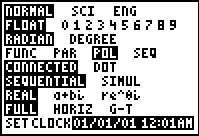
\includegraphics[width=1.8in]{./PolarGraphsGraphics/Polar01.jpg} &
\hspace{0.05in} 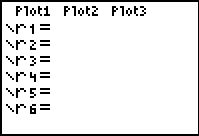
\includegraphics[width=1.8in]{./PolarGraphsGraphics/Polar02.jpg} & 
\hspace{0.05in} 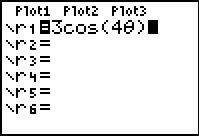
\includegraphics[width=1.8in]{./PolarGraphsGraphics/Polar03.jpg} \\

\end{tabular} 

\end{center}

This changes the ``Y='' menu as seen above in the middle.  Let's plot the polar rose given by $r = 3\cos(4\theta)$ from Exercise \ref{roseexercise8petal} above. We type the function into the ``r='' menu as seen above on the right.  We need to set the viewing window so that the curve displays properly, but when we look at the WINDOW menu, we find three extra lines.

\begin{center}

\begin{tabular}{cc}

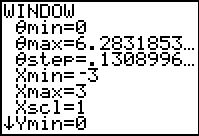
\includegraphics[width=1.8in]{./PolarGraphsGraphics/Polar04.jpg} &
\hspace{0.75in} 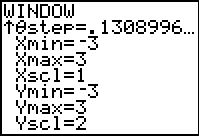
\includegraphics[width=1.8in]{./PolarGraphsGraphics/Polar05.jpg}\\

\end{tabular} 

\end{center}

In order for the calculator to be able to plot $r = 3\cos(4\theta)$ in the $xy$-plane, we need to tell it not only the dimensions which $x$ and $y$ will assume, but we also what values of $\theta$ to use.  From our previous work, we know that we need $0 \leq \theta \leq 2\pi$, so we enter the data you see above.  (I'll say more about the $\theta$-step in just a moment.)  Hitting GRAPH yields the curve below on the left which doesn't look quite right.  The issue here is that the calculator screen is 96 pixels wide but only 64 pixels tall.  To get a true geometric perspective, we need to hit ZOOM SQUARE (seen below in the middle) to produce a more accurate graph which we present below on the right.  

\begin{center}

\begin{tabular}{ccc}

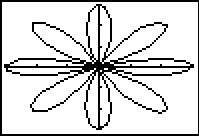
\includegraphics[width=1.8in]{./PolarGraphsGraphics/Polar06.jpg} &
\hspace{0.05in} 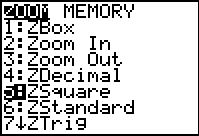
\includegraphics[width=1.8in]{./PolarGraphsGraphics/Polar07.jpg} & 
\hspace{0.05in} 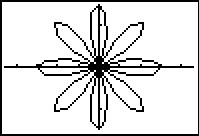
\includegraphics[width=1.8in]{./PolarGraphsGraphics/Polar08.jpg} \\

\end{tabular} 

\end{center}

In function mode, the calculator automatically divided the interval [Xmin, Xmax] into 96 equal subintervals.  In polar mode, however, we must specify how to split up the interval [$\theta$min, $\theta$max] using the $\theta$step.  For most graphs, a $\theta$step of 0.1 is fine.  If you make it too small then the calculator takes a long time to graph.  It you make it too big, you get chunky garbage like this.

\begin{center}

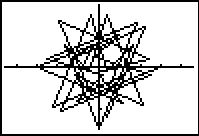
\includegraphics[width=1.8in]{./PolarGraphsGraphics/Polar09.jpg} 

\end{center}

You will need to experiment with the settings in order to get a nice graph.  Exercises \ref{polarcalcfirst} - \ref{polarcalclast} give you some curves to graph using your calculator.  Note some of them have explicit bounds on $\theta$ and others do not.

\begin{multicols}{2}

\begin{enumerate}

\setcounter{enumi}{\value{HW}}

\item $r = \theta, \, 0 \leq \theta \leq 12\pi$ \label{polarcalcfirst}
\item $r = \ln(\theta), \, 1 \leq \theta \leq 12\pi$

\setcounter{HW}{\value{enumi}}

\end{enumerate}

\end{multicols}

\begin{multicols}{2} 

\begin{enumerate}

\setcounter{enumi}{\value{HW}}

\item $r = e^{.1\theta}, \, 0 \leq \theta \leq 12\pi$
\item $r = \theta^{3} - \theta, \, -1.2 \leq \theta \leq 1.2$

\setcounter{HW}{\value{enumi}}

\end{enumerate}

\end{multicols}

\begin{multicols}{2} 

\begin{enumerate}

\setcounter{enumi}{\value{HW}}

\item $r = \sin(5\theta) - 3\cos(\theta)$
\item $r = \sin^{3}\left(\frac{\theta}{2}\right) + \cos^{2}\left(\frac{\theta}{3}\right)$

\setcounter{HW}{\value{enumi}}

\end{enumerate}

\end{multicols}

\begin{multicols}{2} 

\begin{enumerate}

\setcounter{enumi}{\value{HW}}

\item $r = \arctan(\theta), \, -\pi \leq \theta \leq \pi$ \vphantom{$\dfrac{1}{1 - \cos(\theta)}$} 
\item $r = \dfrac{1}{1 - \cos(\theta)}$

\setcounter{HW}{\value{enumi}}

\end{enumerate}

\end{multicols}

\begin{multicols}{2} 

\begin{enumerate}

\setcounter{enumi}{\value{HW}}

\item $r = \dfrac{1}{2 - \cos(\theta)}$
\item $r = \dfrac{1}{2 - 3\cos(\theta)}$ \label{polarcalclast}

\setcounter{HW}{\value{enumi}}

\end{enumerate}

\end{multicols}

\begin{enumerate}

\setcounter{enumi}{\value{HW}}

\item  Use a graphing utility to graph  $r = a - b \sin(\theta)$ for various (positive) values of $a$ and $b$.  Describe the shape of the curve when $a = b$, $a < b$, and when $a > b$.


\item How many petals does the polar rose $r = \sin(2\theta)$ have?  What about $r = \sin(3\theta)$, $r = \sin(4\theta)$ and $r = \sin(5\theta)$?  With the help of your classmates, make a conjecture as to how many petals the polar rose $r = \sin(n\theta)$ has for any natural number $n$.  Replace sine with cosine and repeat the investigation.  How many petals does $r = \cos(n\theta)$ have for each natural number $n$?  


\setcounter{HW}{\value{enumi}}

\end{enumerate}


Looking back through the graphs in the section, it's clear that many polar curves enjoy various forms of symmetry.  However, classifying symmetry for polar curves is not as straight-forward as it was for equations back in Section \ref{Relations}.  In Exercises \ref{sympolarfirst} - \ref{sympolarlast}, we have you and your classmates explore some of the more basic forms of symmetry seen in common polar curves.
\phantomsection
\label{polarsymmetry} 


\begin{enumerate}

\setcounter{enumi}{\value{HW}}

\item Show that if $f$ is even\footnote{Recall that this means $f(-\theta) = f(\theta)$ for $\theta$ in the domain of $f$.} then the graph of $r = f(\theta)$ is symmetric about the $x$-axis. \label{sympolarfirst}

\begin{enumerate}

\item Show that $f(\theta) = 2 + 4\cos(\theta)$ is even and verify that the graph of  $r = 2+4\cos(\theta)$ is indeed symmetric about the $x$-axis.  (See Example \ref{polargraphex} number \ref{limacon02}.)

\item Show that $f(\theta) = 3\sin\left(\frac{\theta}{2}\right)$ is \textbf{not} even, yet the graph of $r = 3\sin\left(\frac{\theta}{2}\right)$ \textbf{is} symmetric about the $x$-axis.  (See  Example \ref{polargraphintex} number \ref{samepolarcurveex}.) 

\end{enumerate}

\item  Show that if $f$ is odd\footnote{Recall that this means $f(-\theta) = -f(\theta)$ for $\theta$ in the domain of $f$.} then the graph of $r = f(\theta)$ is symmetric about the origin.

\begin{enumerate}

\item  Show that $f(\theta) = 5\sin(2\theta)$ is odd and verify that the graph of $r = 5\sin(2\theta)$ is indeed symmetric about the origin.  (See Example \ref{polargraphex} number \ref{rose}.)

\item  Show that $f(\theta) = 3\cos\left(\frac{\theta}{2}\right)$ is \textbf{not} odd, yet the graph of $r = 3\cos\left(\frac{\theta}{2}\right)$ \textbf{is} symmetric about the origin.  (See  Example \ref{polargraphintex} number \ref{samepolarcurveex}.)

\end{enumerate}

\newpage

\item  Show that if $ f(\pi-\theta)=f(\theta)$ for all $\theta$ in the domain of $f$ then the graph of $r = f(\theta)$ is symmetric about the $y$-axis. \label{sympolarlast}

\begin{enumerate}

\item  For $f(\theta) = 4-2\sin(\theta)$, show that $f(\pi - \theta) = f(\theta)$ and the graph of $r = 4-2\sin(\theta)$ is symmetric about the $y$-axis, as required.  (See Example \ref{polargraphex} number \ref{limacon01}.)

\item  For $f(\theta) = 5\sin(2\theta)$, show that $f\left(\pi - \frac{\pi}{4} \right) \neq  f\left(  \frac{\pi}{4} \right)$,  yet the graph of $r = 5\sin(2\theta)$ \textbf{is} symmetric about the $y$-axis.  (See  Example \ref{polargraphex} number  \ref{rose}.)

\end{enumerate}

\setcounter{HW}{\value{enumi}}

\end{enumerate}

In Section \ref{Transformations}, we discussed transformations of graphs.   In Exercise \ref{polargraphtransformations} we have you and your classmates explore transformations of polar graphs. 

\begin{enumerate}

\setcounter{enumi}{\value{HW}}

\item  For Exercises \ref{polargraphexercise1} and \ref{polargraphexercise2} below, let  $f(\theta) = \cos(\theta)$ and $g(\theta) = 2-\sin(\theta)$. \label{polargraphtransformations}

\begin{enumerate}

\item  Using a graphing utility, compare the graph of $r = f(\theta)$ to each of the graphs of $r = f\left(\theta  + \frac{\pi}{4}\right)$, $r = f\left(\theta  + \frac{3\pi}{4}\right)$, $r = f\left(\theta  - \frac{\pi}{4}\right)$ and $r = f\left(\theta  - \frac{3\pi}{4}\right)$.  Repeat this process for $g(\theta)$.  In general, how do you think the graph of $r = f(\theta + \alpha)$ compares with the graph of $r = f(\theta)$?
\label{polargraphexercise1}

\item  Using a graphing utility, compare the graph of $r = f(\theta)$ to each of the graphs of $r = 2f\left(\theta\right)$, $r = \frac{1}{2} f\left(\theta\right)$, $r = -f\left(\theta\right)$ and $r = -3 f(\theta)$.  Repeat this process for $g(\theta)$.  In general, how do you think the graph of $r = k \cdot f(\theta)$ compares with the graph of $r = f(\theta)$? 

Follow up question:  does it matter if $k>0$ or $k<0$?
\label{polargraphexercise2}

\end{enumerate}

\item In light of Exercises \ref{sympolarfirst} - \ref{sympolarlast}, how would the graph of $r = f(-\theta)$ compare with the graph of $r = f(\theta)$ for a generic function $f$?  What about the graphs of $r = -f(\theta)$ and $r = f(\theta)$?  What about $r = f(\theta)$ and $r = f(\pi - \theta)$?  Test out your conjectures using a variety of polar functions found in this section with the help of a graphing utility.

\setcounter{HW}{\value{enumi}}

\end{enumerate}


\begin{enumerate}

\setcounter{enumi}{\value{HW}}

\item With the help of your classmates, research cardioid microphones.

%\item Back in Section \ref{Relations}, in the paragraph before Exercise \ref{listofcurvesfirst}, we gave you this  \href{http://en.wikipedia.org/wiki/List_of_curves}{\underline{link}} to a fascinating list of curves.  Some of these curves have polar representations which we invite you and your classmates to research.

\setcounter{HW}{\value{enumi}}

\end{enumerate}

\newpage

\subsection{Answers}

\begin{multicols}{2} %\raggedcolumns

\begin{enumerate}

\item Circle: $r = 6\sin(\theta)$ 

\begin{mfpic}[15]{-5}{5}{-5}{5}
\axes
\tlabel[cc](5,-0.5){$x$}
\tlabel[cc](0.5,5){$y$}
\xmarks{-4,4}
\ymarks{-4,4}
\tlpointsep{4pt}
\scriptsize
\axislabels {x}{{$-6 \hspace{6pt}$} -4, {$6$} 4}
\axislabels {y}{{$-6$} -4, {$6$} 4}
\normalsize
\penwd{1.25pt}
\plrfcn{0,180,5}{4*sind t}
\end{mfpic} 

\item Circle: $r = 2\cos(\theta)$ 

\begin{mfpic}[15]{-5}{5}{-5}{5}
\axes
\tlabel[cc](5,-0.5){$x$}
\tlabel[cc](0.5,5){$y$}
\xmarks{-4,4}
\ymarks{-4,4}
\tlpointsep{4pt}
\scriptsize
\axislabels {x}{{$-2 \hspace{6pt}$} -4, {$2$} 4}
\axislabels {y}{{$-2$} -4, {$2$} 4}
\normalsize
\penwd{1.25pt}
\plrfcn{0,180,5}{4*cosd t}
\end{mfpic} 

\setcounter{HW}{\value{enumi}}

\end{enumerate}

\end{multicols}

\begin{multicols}{2} 

\begin{enumerate}

\setcounter{enumi}{\value{HW}}

\item Rose: $r = 2\sin(2\theta)$ 

\begin{mfpic}[15]{-5}{5}{-5}{5}
\axes
\tlabel[cc](5,-0.5){$x$}
\tlabel[cc](0.5,5){$y$}
\xmarks{-4,4}
\ymarks{-4,4}
\tlpointsep{4pt}
\scriptsize
\axislabels {x}{{$-2 \hspace{6pt}$} -4, {$2$} 4}
\axislabels {y}{{$-2$} -4, {$2$} 4}
\normalsize
\penwd{1.25pt}
\plrfcn{0,360,5}{4*sind(2*t)}
\end{mfpic} 

\item Rose: $r = 4\cos(2\theta)$ 

\begin{mfpic}[15]{-5}{5}{-5}{5}
\axes
\tlabel[cc](5,-0.5){$x$}
\tlabel[cc](0.5,5){$y$}
\xmarks{-4,4}
\ymarks{-4,4}
\tlpointsep{4pt}
\scriptsize
\axislabels {x}{{$-4 \hspace{6pt}$} -4, {$4$} 4}
\axislabels {y}{{$-4$} -4, {$4$} 4}
\normalsize
\dashed \polyline{(3,3), (-3,-3)}
\gclear \tlabelrect(3,3){\scriptsize $\theta = \frac{\pi}{4}$}
\dashed \polyline{(3,-3), (-3,3)}
\gclear \tlabelrect(-3,3){\scriptsize $\theta = \frac{3\pi}{4}$}
\penwd{1.25pt}
\plrfcn{0,360,5}{4*cosd(2*t)}
\end{mfpic} 

\setcounter{HW}{\value{enumi}}

\end{enumerate}

\end{multicols}

\begin{multicols}{2} 

\begin{enumerate}

\setcounter{enumi}{\value{HW}}

\item Rose: $r = 5\sin(3\theta)$ 

\begin{mfpic}[15]{-5}{5}{-5}{5}
\axes
\tlabel[cc](5,-0.5){$x$}
\tlabel[cc](0.5,5){$y$}
\xmarks{-4,4}
\ymarks{-4,4}
\tlpointsep{4pt}
\scriptsize
\axislabels {x}{{$-5 \hspace{6pt}$} -4, {$5$} 4}
\axislabels {y}{{$-5$} -4, {$5$} 4}
\normalsize
\dashed \polyline{(2,3.464), (-2,-3.464)}
\gclear \tlabelrect(2,3.464){\scriptsize $\theta = \frac{\pi}{3}$}
\dashed \polyline{(-2,3.464), (2,-3.464)}
\gclear \tlabelrect(-2,3.464){\scriptsize $\theta = \frac{2\pi}{3}$}
\penwd{1.25pt}
\plrfcn{0,180,5}{4*sind(3*t)}
\end{mfpic} 

\item Rose: $r = \cos(5\theta)$ 

\begin{mfpic}[15]{-5}{5}{-5}{5}
\axes
\tlabel[cc](5,-0.5){$x$}
\tlabel[cc](0.5,5){$y$}
\xmarks{-4,4}
\ymarks{-4,4}
\tlpointsep{4pt}
\scriptsize
\axislabels {x}{{$-1 \hspace{6pt}$} -4, {$1$} 4}
\axislabels {y}{{$-1$} -4, {$1$} 4}
\normalsize
\dashed \polyline{(3.804,1.236), (-3.804,-1.236)}
\gclear \tlabelrect(3.804,1.236){\scriptsize $\theta = \frac{\pi}{10}$}
\dashed \polyline{(2.351,3.236), (-2.351,-3.236)}
\gclear \tlabelrect(2.351,3.236){\scriptsize $\theta = \frac{3\pi}{10}$}
\dashed \polyline{(-2.351,3.236), (2.351,-3.236)}
\gclear \tlabelrect(-2.351,3.236){\scriptsize $\theta = \frac{7\pi}{10}$}
\dashed \polyline{(-3.804,1.236), (3.804,-1.236)}
\gclear \tlabelrect(-3.804,1.236){\scriptsize $\theta = \frac{9\pi}{10}$}
\penwd{1.25pt}
\plrfcn{0,180,5}{4*cosd(5*t)}
\end{mfpic} 

\setcounter{HW}{\value{enumi}}

\end{enumerate}

\end{multicols}

\begin{multicols}{2} 

\begin{enumerate}

\setcounter{enumi}{\value{HW}}

\item Rose: $r = \sin(4\theta)$ 

\begin{mfpic}[15]{-5}{5}{-5}{5}
\axes
\tlabel[cc](5,-0.5){$x$}
\tlabel[cc](0.5,5){$y$}
\xmarks{-4,4}
\ymarks{-4,4}
\tlpointsep{4pt}
\scriptsize
\axislabels {x}{{$-1 \hspace{6pt}$} -4, {$1$} 4}
\axislabels {y}{{$-1$} -4, {$1$} 4}
\normalsize
\dashed \polyline{(3,3), (-3,-3)}
\gclear \tlabelrect(3,3){\scriptsize $\theta = \frac{\pi}{4}$}
\dashed \polyline{(3,-3), (-3,3)}
\gclear \tlabelrect(-3,3){\scriptsize $\theta = \frac{3\pi}{4}$}
\penwd{1.25pt}
\plrfcn{0,360,5}{4*sind(4*t)}
\end{mfpic} 

\item Rose: $r = 3\cos(4\theta)$ 

\begin{mfpic}[15]{-5}{5}{-5}{5}
\axes
\tlabel[cc](5,-0.5){$x$}
\tlabel[cc](0.5,5){$y$}
\xmarks{-4,4}
\ymarks{-4,4}
\tlpointsep{4pt}
\scriptsize
\axislabels {x}{{$-3 \hspace{6pt}$} -4, {$3$} 4}
\axislabels {y}{{$-3$} -4, {$3$} 4}
\normalsize
\dashed \polyline{(3.696,1.531), (-3.696,-1.531)}
\gclear \tlabelrect(3.696,1.531){\scriptsize $\theta = \frac{\pi}{8}$}
\dashed \polyline{(1.531,3.696), (-1.531,-3.696)}
\gclear \tlabelrect(1.531,3.696){\scriptsize $\theta = \frac{3\pi}{8}$}
\dashed \polyline{(-1.531,3.696), (1.531,-3.696)}
\gclear \tlabelrect(-1.531,3.696){\scriptsize $\theta = \frac{5\pi}{8}$}
\dashed \polyline{(-3.696,1.531), (3.696,-1.531)}
\gclear \tlabelrect(-3.696,1.531){\scriptsize $\theta = \frac{7\pi}{8}$}
\penwd{1.25pt}
\plrfcn{0,360,5}{4*cosd(4*t)}
\end{mfpic} 

\setcounter{HW}{\value{enumi}}

\end{enumerate}

\end{multicols}

\begin{multicols}{2} 

\begin{enumerate}

\setcounter{enumi}{\value{HW}}

\item Cardioid: $r = 3 - 3\cos(\theta)$ 

\begin{mfpic}[15]{-5}{5}{-5}{5}
\axes
\tlabel[cc](5,-0.5){$x$}
\tlabel[cc](0.5,5){$y$}
\xmarks{-4,-2,2,4}
\ymarks{-4,-2,2,4}
\tlpointsep{4pt}
\scriptsize
\axislabels {x}{{$-6 \hspace{6pt}$} -4, {$-3 \hspace{6pt}$} -2, {$3$} 2, {$6$} 4}
\axislabels {y}{{$-6$} -4, {$-3$} -2, {$3$} 2, {$6$} 4}
\normalsize
\penwd{1.25pt}
\plrfcn{0,360,5}{2 - 2*cosd(t)}
\end{mfpic} 

\item Cardioid: $r = 5 + 5\sin(\theta)$ 

\begin{mfpic}[15]{-5}{5}{-5}{5}
\axes
\tlabel[cc](5,-0.5){$x$}
\tlabel[cc](0.5,5){$y$}
\xmarks{-4,-2,2,4}
\ymarks{-4,-2,2,4}
\tlpointsep{4pt}
\scriptsize
\axislabels {x}{{$-10 \hspace{6pt}$} -4, {$-5 \hspace{6pt}$} -2, {$5$} 2, {$10$} 4}
\axislabels {y}{{$-10$} -4, {$-5$} -2, {$5$} 2, {$10$} 4}
\normalsize
\penwd{1.25pt}
\plrfcn{0,360,5}{2 + 2*sind(t)}
\end{mfpic} 

\setcounter{HW}{\value{enumi}}

\end{enumerate}

\end{multicols}

\begin{multicols}{2} 

\begin{enumerate}

\setcounter{enumi}{\value{HW}}

\item Cardioid: $r = 2 + 2\cos(\theta)$ 

\begin{mfpic}[15]{-5}{5}{-5}{5}
\axes
\tlabel[cc](5,-0.5){$x$}
\tlabel[cc](0.5,5){$y$}
\xmarks{-4,-2,2,4}
\ymarks{-4,-2,2,4}
\tlpointsep{4pt}
\scriptsize
\axislabels {x}{{$-4 \hspace{6pt}$} -4, {$-2 \hspace{6pt}$} -2, {$2$} 2, {$4$} 4}
\axislabels {y}{{$-4$} -4, {$-2$} -2, {$2$} 2, {$4$} 4}
\normalsize
\penwd{1.25pt}
\plrfcn{0,360,5}{2 + 2*cosd(t)}
\end{mfpic} 

\item Cardioid: $r = 1 - \sin(\theta)$ 

\begin{mfpic}[15]{-5}{5}{-5}{5}
\axes
\tlabel[cc](5,-0.5){$x$}
\tlabel[cc](0.5,5){$y$}
\xmarks{-4,-2,2,4}
\ymarks{-4,-2,2,4}
\tlpointsep{4pt}
\scriptsize
\axislabels {x}{{$-2 \hspace{6pt}$} -4, {$-1 \hspace{6pt}$} -2, {$1$} 2, {$2$} 4}
\axislabels {y}{{$-2$} -4, {$-1$} -2, {$1$} 2, {$2$} 4}
\normalsize
\penwd{1.25pt}
\plrfcn{0,360,5}{2 - 2*sind(t)}
\end{mfpic} 

\setcounter{HW}{\value{enumi}}

\end{enumerate}

\end{multicols}

\begin{multicols}{2} 

\begin{enumerate}

\setcounter{enumi}{\value{HW}}

\item Lima\c{c}on: $r = 1 - 2\cos(\theta)$ 

\begin{mfpic}[15]{-5}{5}{-5}{5}
\axes
\tlabel[cc](5,-0.5){$x$}
\tlabel[cc](0.5,5){$y$}
\xmarks{-4,-1.3333,1.3333,4}
\ymarks{-4,-1.3333,1.3333,4}
\tlpointsep{4pt}
\scriptsize
\axislabels {x}{{$-3 \hspace{6pt}$} -4, {$-1 \hspace{6pt}$} -1.3333, {$1$} 1.3333, {$3$} 4}
\axislabels {y}{{$-3$} -4, {$-1$} -1.3333, {$1$} 1.3333, {$3$} 4}
\normalsize
\dashed \polyline{(0,0), (2,3.464)}
\gclear \tlabelrect(2,3.464){\scriptsize $\theta = \frac{\pi}{3}$}
\dashed \polyline{(0,0), (2,-3.464)}
\gclear \tlabelrect(2,-3.464){\scriptsize $\theta = \frac{5\pi}{3}$}
\penwd{1.25pt}
\plrfcn{0,360,5}{1.3333*(1 - 2*cosd(t))}
\end{mfpic} 

\item Lima\c{c}on: $r = 1 - 2\sin(\theta)$ 

\begin{mfpic}[15]{-5}{5}{-5}{5}
\axes
\tlabel[cc](5,-0.5){$x$}
\tlabel[cc](0.5,5){$y$}
\xmarks{-4,-1.3333,1.3333,4}
\ymarks{-4,-1.3333,1.3333,4}
\tlpointsep{4pt}
\scriptsize
\axislabels {x}{{$-3 \hspace{6pt}$} -4, {$-1 \hspace{6pt}$} -1.3333, {$1$} 1.3333, {$3$} 4}
\axislabels {y}{{$-3$} -4, {$-1$} -1.3333, {$1$} 1.3333, {$3$} 4}
\normalsize
\dashed \polyline{(0,0), (3.464,2)}
\gclear \tlabelrect(3.464,2){\scriptsize $\theta = \frac{\pi}{6}$}
\dashed \polyline{(0,0), (-3.464,2)}
\gclear \tlabelrect(-3.464,2){\scriptsize $\theta = \frac{5\pi}{6}$}
\penwd{1.25pt}
\plrfcn{0,360,5}{1.3333*(1 - 2*sind(t))}
\end{mfpic} 

\setcounter{HW}{\value{enumi}}

\end{enumerate}

\end{multicols}

\begin{multicols}{2} 

\begin{enumerate}

\setcounter{enumi}{\value{HW}}

\item Lima\c{c}on: $r = 2\sqrt{3} + 4\cos(\theta)$ 

\begin{mfpic}[15]{-5}{5}{-5}{5}
\axes
\tlabel[cc](5,0.5){$x$}
\tlabel[cc](0.5,5){$y$}
\xmarks{-4,-1.856,1.856,4}
\ymarks{-4,4}
\tlpointsep{4pt}
\scriptsize
\axislabels {x}{{$-2\sqrt{3} - 4 \hspace{6pt}$} -4, {$2\sqrt{3} + 4$} 4}
\axislabels {y}{{$-2\sqrt{3} - 4$} -4, {$-2\sqrt{3}$} -1.856, {$2\sqrt{3}$} 1.856, {$2\sqrt{3} + 4$} 4}
\normalsize
\dashed \polyline{(0,0), (-3.464,-2)}
\gclear \tlabelrect(-3.464,-2){\scriptsize $\theta = \frac{7\pi}{6}$}
\dashed \polyline{(0,0), (-3.464,2)}
\gclear \tlabelrect(-3.464,2){\scriptsize $\theta = \frac{5\pi}{6}$}
\penwd{1.25pt}
\plrfcn{0,360,5}{1.0718*(1.73205 + 2*cosd(t))}
\end{mfpic} 

\item Lima\c{c}on: $r = 3-5\cos(\theta)$ 

\begin{mfpic}[15]{-5}{5}{-5}{5}
\axes
\tlabel[cc](5,-0.5){$x$}
\tlabel[cc](0.5,5){$y$}
\xmarks{-4,-1,4}
\ymarks{-4,-1.5,1.5,4}
\tlpointsep{4pt}
\scriptsize
\axislabels {y}{{$-8$} -4, {$-3$} -1.5, {$3$} 1.5, {$8$} 4}
\axislabels {x}{{$-8 \hspace{6pt}$} -4, {$-2 \hspace{6pt}$} -1, {$8$} 4}
\normalsize
\dashed \polyline{(0,0), (2.41,3.19)}
\gclear \tlabelrect(2.9,3.3){\tiny $\theta = \arccos\left(\frac{3}{5}\right)$}
\dashed \polyline{(0,0), (2.41,-3.19)}
\gclear \tlabelrect(2.9,-3.3){\tiny $\theta = 2\pi - \arccos\left(\frac{3}{5}\right)$}
\penwd{1.25pt}
\plrfcn{0,360,5}{0.5*(3 - 5*cosd(t))}
\end{mfpic} 

\setcounter{HW}{\value{enumi}}

\end{enumerate}

\end{multicols}

\begin{multicols}{2} 

\begin{enumerate}

\setcounter{enumi}{\value{HW}}

\item Lima\c{c}on: $r = 3-5\sin(\theta)$ 

\begin{mfpic}[15]{-5}{5}{-5}{5}
\axes
\tlabel[cc](5,-0.5){$x$}
\tlabel[cc](0.5,5){$y$}
\xmarks{-4,-1.5,1.5,4}
\ymarks{-4,-1,4}
\tlpointsep{4pt}
\scriptsize
\axislabels {x}{{$-8 \hspace{6pt}$} -4, {$-3 \hspace{6pt}$} -1.5, {$3$} 1.5, {$8$} 4}
\axislabels {y}{{$-8$} -4, {$-2$} -1, {$8$} 4}
\normalsize
\dashed \polyline{(0,0), (3.2,2.4)}
\gclear \tlabelrect(2.9,3){\tiny $\theta = \arcsin\left(\frac{3}{5}\right)$}
\dashed \polyline{(0,0), (-3.2,2.4)}
\gclear \tlabelrect(-2.9,3){\tiny $\theta = \pi - \arcsin\left(\frac{3}{5}\right)$}
\penwd{1.25pt}
\plrfcn{0,360,5}{0.5*(3 - 5*sind(t))}
\end{mfpic} 

\item Lima\c{c}on: $r = 2 + 7\sin(\theta)$ 

\begin{mfpic}[15]{-5}{5}{-5}{5}
\axes
\tlabel[cc](5,-0.5){$x$}
\tlabel[cc](0.5,5){$y$}
\xmarks{-4,-0.8888,0.8888,4}
\ymarks{-4,2.2222,4}
\tlpointsep{4pt}
\scriptsize
\axislabels {x}{{$-9 \hspace{6pt}$} -4, {$-2 \hspace{6pt}$} -0.8888, {$2$} 0.8888, {$9$} 4}
\axislabels {y}{{$-9$} -4, {$5$} 2.2222, {$9$} 4}
\normalsize
\dashed \polyline{(0,0), (-3.842,-1.113)}
\gclear \tlabelrect(-2.9,-1.3){\tiny $\theta = \pi + \arcsin\left(\frac{2}{7}\right)$}
\dashed \polyline{(0,0), (3.842,-1.113)}
\gclear \tlabelrect(2.9,-1.3){\tiny $\theta = 2\pi - \arcsin\left(\frac{2}{7}\right)$}
\penwd{1.25pt}
\plrfcn{0,360,5}{0.4444*(2 + 7*sind(t))}
\end{mfpic} 

\setcounter{HW}{\value{enumi}}

\end{enumerate}

\end{multicols}

\begin{multicols}{2} 

\begin{enumerate}

\setcounter{enumi}{\value{HW}}

\item Lemniscate: $r^{2} = \sin(2\theta)$ 

\begin{mfpic}[15]{-5}{5}{-5}{5}
\axes
\tlabel[cc](5,-0.5){$x$}
\tlabel[cc](0.5,5){$y$}
\xmarks{-4,4}
\ymarks{-4,4}
\tlpointsep{4pt}
\scriptsize
\axislabels {x}{{$-1 \hspace{6pt}$} -4, {$1$} 4}
\axislabels {y}{{$-1$} -4, {$1$} 4}
\normalsize
\penwd{1.25pt}
\plrfcn{0,90,5}{4*sqrt(sind(2*t))}
\plrfcn{180,270,5}{4*sqrt(sind(2*t))}
\end{mfpic} 

\item Lemniscate: $r^{2} = 4\cos(2\theta)$ 

\begin{mfpic}[15]{-5}{5}{-5}{5}
\axes
\tlabel[cc](5,-0.5){$x$}
\tlabel[cc](0.5,5){$y$}
\xmarks{-4,4}
\ymarks{-4,4}
\tlpointsep{4pt}
\scriptsize
\axislabels {x}{{$-2 \hspace{6pt}$} -4, {$2$} 4}
\axislabels {y}{{$-2$} -4, {$2$} 4}
\normalsize
\dashed \polyline{(3,3), (-3,-3)}
\gclear \tlabelrect(3,3){\scriptsize $\theta = \frac{\pi}{4}$}
\dashed \polyline{(3,-3), (-3,3)}
\gclear \tlabelrect(-3,3){\scriptsize $\theta = \frac{3\pi}{4}$}
\penwd{1.25pt}
\plrfcn{-45,45,5}{4*sqrt(cosd(2*t))}
\plrfcn{135,225,5}{4*sqrt(cosd(2*t))}
\end{mfpic} 

\setcounter{HW}{\value{enumi}}

\end{enumerate}

\end{multicols}

\begin{enumerate}

\setcounter{enumi}{\value{HW}}

\item \begin{multicols}{2} \raggedcolumns

$r = 3\cos(\theta)$ and $r = 1 + \cos(\theta)$

\begin{mfpic}[17]{-4}{4}{-4}{4}
\axes
\tlabel[cc](4,-0.5){$x$}
\tlabel[cc](0.5,4){$y$}
\xmarks{-3,-2,-1,1,2,3}
\ymarks{-3,-2,-1,1,2,3}
\tlpointsep{4pt}
\scriptsize
\axislabels {x}{{$-3 \hspace{6pt}$} -3, {$-2 \hspace{6pt}$} -2, {$-1 \hspace{6pt}$} -1, {$1$} 1, {$2$} 2, {$3$} 3}
\axislabels {y}{{$-3$} -3, {$-2$} -2, {$-1$} -1, {$1$} 1, {$2$} 2, {$3$} 3}
\normalsize
\penwd{1.25pt}
\plrfcn{0,360,5}{1 + cosd(t)}
\plrfcn{0,360,5}{3*cosd(t)}
\end{mfpic} 

$\left( \dfrac{3}{2}, \dfrac{\pi}{3} \right)$, $\left( \dfrac{3}{2}, \dfrac{5\pi}{3} \right)$, pole

\end{multicols}

\item \begin{multicols}{2} \raggedcolumns 

$r = 1 + \sin(\theta)$ and $r = 1 - \cos(\theta)$

\begin{mfpic}[23]{-2.9}{3}{-3}{3}
\axes
\tlabel[cc](3,-0.5){$x$}
\tlabel[cc](0.5,3){$y$}
\xmarks{-2,-1,1,2}
\ymarks{-2,-1,1,2}
\tlpointsep{4pt}
\scriptsize
\axislabels {x}{{$-2 \hspace{6pt}$} -2, {$-1 \hspace{6pt}$} -1, {$1$} 1, {$2$} 2}
\axislabels {y}{{$-2$} -2, {$-1$} -1, {$1$} 1, {$2$} 2}
\normalsize
\penwd{1.25pt}
\plrfcn{0,360,5}{1 - cosd(t)}
\plrfcn{0,360,5}{1 + sind(t)}
\end{mfpic} 

$\left( \dfrac{2 + \sqrt{2}}{2}, \dfrac{3\pi}{4} \right)$, $\left( \dfrac{2 - \sqrt{2}}{2}, \dfrac{7\pi}{4} \right)$, pole

\end{multicols}

\pagebreak

\item \begin{multicols}{2} \raggedcolumns 

$r = 1 - 2\sin(\theta)$ and $r = 2$

\begin{mfpic}[15]{-5}{5}{-5}{5}
\axes
\tlabel[cc](5,-0.5){$x$}
\tlabel[cc](0.5,5){$y$}
\xmarks{-4,-1.3333,1.3333,4}
\ymarks{-4,-1.3333,1.3333,4}
\tlpointsep{4pt}
\scriptsize
\axislabels {x}{{$-3 \hspace{6pt}$} -4, {$-1 \hspace{6pt}$} -1.3333, {$1$} 1.3333, {$3$} 4}
\axislabels {y}{{$-3$} -4, {$-1$} -1.3333, {$1$} 1.3333, {$3$} 4}
\normalsize
\penwd{1.25pt}
\plrfcn{0,360,5}{1.3333*(1 - 2*sind(t))}
\circle{(0,0),2}
\end{mfpic} 

$\left( 2, \dfrac{7\pi}{6} \right)$, $\left( 2, \dfrac{11\pi}{6} \right)$

\end{multicols}

\item \begin{multicols}{2} \raggedcolumns 

$r = 1 - 2\cos(\theta)$ and $r = 1$

\begin{mfpic}[15]{-5}{5}{-5}{5}
\axes
\tlabel[cc](5,-0.5){$x$}
\tlabel[cc](0.5,5){$y$}
\xmarks{-4,-1.3333,1.3333,4}
\ymarks{-4,-1.3333,1.3333,4}
\tlpointsep{4pt}
\scriptsize
\axislabels {x}{{$-3 \hspace{6pt}$} -4, {$-1 \hspace{6pt}$} -1.3333, {$1$} 1.3333, {$3$} 4}
\axislabels {y}{{$-3$} -4, {$-1$} -1.3333, {$1$} 1.3333, {$3$} 4}
\normalsize
\penwd{1.25pt}
\plrfcn{0,360,5}{1.3333*(1 - 2*cosd(t))}
\plrfcn{0,360,5}{1.3333}
\end{mfpic} 

$\left( 1, \dfrac{\pi}{2} \right)$, $\left( 1, \dfrac{3\pi}{2} \right)$, $(-1, 0)$

\end{multicols}

\item \begin{multicols}{2} \raggedcolumns  

$r = 2\cos(\theta)$ and $r = 2\sqrt{3} \sin(\theta)$

\begin{mfpic}[19]{-4}{4}{-5}{5}
\axes
\tlabel[cc](4,-0.5){$x$}
\tlabel[cc](0.5,5){$y$}
\xmarks{-3,-2,-1,1,2,3}
\ymarks{-4,-3,-2,-1,1,2,3,4}
\tlpointsep{4pt}
\scriptsize
\axislabels {x}{{$-3 \hspace{6pt}$} -3, {$-2 \hspace{6pt}$} -2, {$-1 \hspace{6pt}$} -1, {$1$} 1, {$2$} 2, {$3$} 3}
\axislabels {y}{{$-4$} -4,{$-3$} -3, {$-2$} -2, {$-1$} -1, {$1$} 1, {$2$} 2, {$3$} 3, {$4$} 4}
\normalsize
\penwd{1.25pt}
\plrfcn{0,360,5}{3.46*sind(t)}
\plrfcn{0,360,5}{2*cosd(t)}
\end{mfpic} 

$\left(\sqrt{3}, \dfrac{\pi}{6} \right)$, pole

\end{multicols}


\item \begin{multicols}{2} \raggedcolumns  

$r = 3\cos(\theta)$ and $r = \sin(\theta)$

\begin{mfpic}[19]{-4}{4}{-4}{4}
\axes
\tlabel[cc](4,-0.5){$x$}
\tlabel[cc](0.5,4){$y$}
\xmarks{-3,-2,-1,1,2,3}
\ymarks{-3,-2,-1,1,2,3}
\tlpointsep{4pt}
\scriptsize
\axislabels {x}{{$-3 \hspace{6pt}$} -3, {$-2 \hspace{6pt}$} -2, {$-1 \hspace{6pt}$} -1, {$1$} 1, {$2$} 2, {$3$} 3}
\axislabels {y}{{$-3$} -3, {$-2$} -2, {$-1$} -1, {$1$} 1, {$2$} 2, {$3$} 3}
\normalsize
\penwd{1.25pt}
\plrfcn{0,360,5}{sind(t)}
\plrfcn{0,360,5}{3*cosd(t)}
\end{mfpic} 

$\left(\dfrac{3\sqrt{10}}{10}, \arctan(3)\right)$, pole

\end{multicols}

\item \begin{multicols}{2} \raggedcolumns 

$r^2 = 4\cos(2\theta)$ and $r = \sqrt{2}$

\begin{mfpic}[15]{-5}{5}{-5}{5}
\axes
\tlabel[cc](5,-0.5){$x$}
\tlabel[cc](0.5,5){$y$}
\xmarks{-4,4}
\ymarks{-4,4}
\tlpointsep{4pt}
\scriptsize
\axislabels {x}{{$-2 \hspace{6pt}$} -4, {$2$} 4}
\axislabels {y}{{$-2$} -4, {$2$} 4}
\normalsize
\penwd{1.25pt}
\plrfcn{-45,45,5}{4*sqrt(cosd(2*t))}
\plrfcn{135,225,5}{4*sqrt(cosd(2*t))}
\circle{(0,0), 1.414}

\end{mfpic} 

$\left(\sqrt{2}, \dfrac{\pi}{6}\right)$, $\left(\sqrt{2}, \dfrac{5\pi}{6}\right)$, $\left(\sqrt{2}, \dfrac{7\pi}{6}\right)$, $\left(\sqrt{2}, \dfrac{11\pi}{6}\right)$

\end{multicols}

\item \begin{multicols}{2} \raggedcolumns 

$r^{2} = 2\sin(2\theta)$ and $r = 1$

\begin{mfpic}[15]{-5}{5}{-5}{5}
\axes
\tlabel[cc](5,-0.5){$x$}
\tlabel[cc](0.5,5){$y$}
\xmarks{-4,4}
\ymarks{-4,4}
\tlpointsep{4pt}
\scriptsize
\axislabels {x}{{\tiny $-\sqrt{2} \hspace{6pt}$} -4, {$-1 \hspace{6pt}$} -2.828, {$1$} 2.828, {\tiny $\sqrt{2}$} 4}
\axislabels {y}{{\tiny $-\sqrt{2}$} -4, {$-1$} -2.828, {$1$} 2.828, {\tiny $\sqrt{2}$} 4}
\normalsize
\penwd{1.25pt}
\plrfcn{0,90,5}{4*sqrt(sind(2*t))}
\plrfcn{180,270,5}{4*sqrt(sind(2*t))}
\plrfcn{0,360,5}{2.828}
\end{mfpic} 

$\left(1, \dfrac{\pi}{12}\right)$, $\left(1, \dfrac{5\pi}{12}\right)$, $\left(1, \dfrac{13\pi}{12}\right)$, $\left(1, \dfrac{17\pi}{12}\right)$

\end{multicols}

\pagebreak

\item \begin{multicols}{2} \raggedcolumns

 $r = 4\cos(2\theta)$  and $r = 2$

\begin{mfpic}[15]{-5}{5}{-5}{5}
\axes
\tlabel[cc](5,-0.5){$x$}
\tlabel[cc](0.5,5){$y$}
\xmarks{-4,4}
\ymarks{-4,4}
\tlpointsep{4pt}
\scriptsize
\axislabels {x}{{$-4 \hspace{6pt}$} -4, {$4$} 4}
\axislabels {y}{{$-4$} -4, {$4$} 4}
\normalsize
\penwd{1.25pt}
\plrfcn{0,360,5}{4*cosd(2*t)}
\circle{(0,0),2}

\end{mfpic} 

$\left( 2, \dfrac{\pi}{6} \right)$, $\left( 2, \dfrac{5\pi}{6} \right)$, $\left( 2, \dfrac{7\pi}{6} \right)$, 

$\left( 2, \dfrac{11\pi}{6} \right)$, $\left( -2, \dfrac{\pi}{3} \right)$, $\left( -2, \dfrac{2\pi}{3} \right)$, 

$\left( -2, \dfrac{4\pi}{3} \right)$, $\left( -2, \dfrac{5\pi}{3} \right)$

\end{multicols}

\item \begin{multicols}{2} \raggedcolumns

$r = 2\sin(2\theta)$ and $r = 1$

\begin{mfpic}[15]{-4.5}{5}{-5}{5}
\axes
\tlabel[cc](5,-0.5){$x$}
\tlabel[cc](0.5,5){$y$}
\xmarks{-4,4}
\ymarks{-4,4}
\tlpointsep{4pt}
\scriptsize
\axislabels {x}{{$-2 \hspace{6pt}$} -4, {$2$} 4}
\axislabels {y}{{$-2$} -4, {$2$} 4}
\normalsize
\penwd{1.25pt}
\plrfcn{0,360,5}{4*sind(2*t)}
\plrfcn{0,360,5}{2}
\end{mfpic} 

$\left( 1, \dfrac{\pi}{12} \right)$, $\left( 1, \dfrac{5\pi}{12} \right)$, $\left( 1, \dfrac{13\pi}{12} \right)$, 

$\left( 1, \dfrac{17\pi}{12} \right)$, $\left( -1, \dfrac{7\pi}{12} \right)$, $\left( -1, \dfrac{11\pi}{12} \right)$, 

$\left( -1, \dfrac{19\pi}{12} \right)$, $\left( -1, \dfrac{23\pi}{12} \right)$

\end{multicols}

\setcounter{HW}{\value{enumi}}

\end{enumerate}

\pagebreak

\begin{multicols}{2}

\begin{enumerate}

\setcounter{enumi}{\value{HW}}

\item $\left\{ (r,\theta) \, | \, 0 \leq r \leq 3, \,0 \leq \theta \leq 2\pi \right\}$

\begin{mfpic}[15]{-5}{5}{-5}{5}
\fillcolor[gray]{0.7}
\gfill \circle{(0,0),3}
\axes
\tlabel[cc](5,-0.5){$x$}
\tlabel[cc](0.5,5){$y$}
\xmarks{-3,-2,-1,1,2,3}
\ymarks{-3,-2,-1,1,2,3}
\tlpointsep{4pt}
\scriptsize
\axislabels {x}{{$-3 \hspace{6pt}$} -3, {$-2 \hspace{6pt}$} -2, {$-1 \hspace{6pt}$} -1, {$1$} 1, {$2$} 2, {$3$} 3}
\axislabels {y}{{$-3$} -3, {$-2$} -2, {$-1$} -1, {$1$} 1, {$2$} 2, {$3$} 3}
\normalsize
\penwd{1.25pt}
\circle{(0,0),3}
\end{mfpic} 

\item $\left\{ (r,\theta) \, | \, 0 \leq r \leq 4\sin(\theta), \,0 \leq \theta \leq \pi \right\}$

\begin{mfpic}[15]{-5}{5}{-5}{5}
\fillcolor[gray]{0.7}
\gfill \plrregion{0,180,1}{4*sind(t)}
\axes
\tlabel[cc](5,-0.5){$x$}
\tlabel[cc](0.5,5){$y$}
\xmarks{-4,-3,-2,-1,1,2,3,4}
\ymarks{-4,-3,-2,-1,1,2,3,4}
\tlpointsep{4pt}
\scriptsize
\axislabels {x}{{$-4 \hspace{6pt}$} -4,{$-3 \hspace{6pt}$} -3, {$-2 \hspace{6pt}$} -2, {$-1 \hspace{6pt}$} -1, {$1$} 1, {$2$} 2, {$3$} 3, {$4$} 4}
\axislabels {y}{{$-4$} -4,{$-3$} -3, {$-2$} -2, {$-1$} -1, {$1$} 1, {$2$} 2, {$3$} 3, {$4$} 4}
\normalsize
\penwd{1.25pt}
\plrfcn{0,180,5}{4*sind(t)}
\end{mfpic} 

\setcounter{HW}{\value{enumi}}

\end{enumerate}

\end{multicols}

\begin{multicols}{2} 

\begin{enumerate}

\setcounter{enumi}{\value{HW}}

\item $\left\{ (r,\theta) \, | \, 0 \leq r \leq 3\cos(\theta), \, -\frac{\pi}{2} \leq \theta \leq \frac{\pi}{2} \right\}$

\begin{mfpic}[15]{-5}{5}{-5}{5}
\fillcolor[gray]{0.7}
\gfill \plrregion{-90,90,1}{3*cosd(t)}
\axes
\tlabel[cc](5,-0.5){$x$}
\tlabel[cc](0.5,5){$y$}
\xmarks{-3,-2,-1,1,2,3}
\ymarks{-3,-2,-1,1,2,3}
\tlpointsep{4pt}
\scriptsize
\axislabels {x}{{$-3 \hspace{6pt}$} -3, {$-2 \hspace{6pt}$} -2, {$-1 \hspace{6pt}$} -1, {$1$} 1, {$2$} 2, {$3$} 3}
\axislabels {y}{{$-3$} -3, {$-2$} -2, {$-1$} -1, {$1$} 1, {$2$} 2, {$3$} 3}
\normalsize
\penwd{1.25pt}
\plrfcn{-90,90,5}{3*cosd(t)}
\end{mfpic} 

\item $\left\{ (r,\theta) \, | \,  0 \leq r \leq 2\sin(2\theta), \,0 \leq \theta \leq \frac{\pi}{2} \right\}$

\begin{mfpic}[15]{-5}{5}{-5}{5}
\fillcolor[gray]{0.7}
\gfill \plrregion{0,90,5}{4*sind(2*t)}
\axes
\tlabel[cc](5,-0.5){$x$}
\tlabel[cc](0.5,5){$y$}
\xmarks{-4,4}
\ymarks{-4,4}
\tlpointsep{4pt}
\scriptsize
\axislabels {x}{{$-2 \hspace{6pt}$} -4, {$2$} 4}
\axislabels {y}{{$-2$} -4, {$2$} 4}
\normalsize
\penwd{1.25pt}
\plrfcn{0,360,5}{4*sind(2*t)}
\end{mfpic} 

\setcounter{HW}{\value{enumi}}

\end{enumerate}

\end{multicols}

\begin{multicols}{2} 

\begin{enumerate}

\setcounter{enumi}{\value{HW}}

\item $\left\{ (r,\theta) \, | \, 0 \leq r \leq 4\cos(2\theta), \, -\frac{\pi}{4} \leq \theta \leq \frac{\pi}{4} \right\}$

\begin{mfpic}[15]{-5}{5}{-5}{5}
\fillcolor[gray]{0.7}
\gfill \plrregion{-45,45,5}{4*cosd(2*t)}
\axes
\tlabel[cc](5,-0.5){$x$}
\tlabel[cc](0.5,5){$y$}
\xmarks{-4,4}
\ymarks{-4,4}
\tlpointsep{4pt}
\scriptsize
\axislabels {x}{{$-4 \hspace{6pt}$} -4, {$4$} 4}
\axislabels {y}{{$-4$} -4, {$4$} 4}
\normalsize
\penwd{1.25pt}
\plrfcn{0,360,5}{4*cosd(2*t)}
\end{mfpic} 

\item $\left\{ (r,\theta) \, | \, 1 \leq r \leq 1-2\cos(\theta), \, \frac{\pi}{2} \leq \theta \leq \frac{3\pi}{2} \right\}$

\begin{mfpic}[15]{-5}{5}{-5}{5}
\fillcolor[gray]{0.7}
\gfill \plrregion{90,270,5}{1.3333*(1 - 2*cosd(t))}
\gclear \plrregion{90,270,5}{1.3333}
\axes
\tlabel[cc](5,-0.5){$x$}
\tlabel[cc](0.5,5){$y$}
\xmarks{-4,-1.3333,1.3333,4}
\ymarks{-4,-1.3333,1.3333,4}
\tlpointsep{4pt}
\scriptsize
\axislabels {x}{{$-3 \hspace{6pt}$} -4, {$-1 \hspace{6pt}$} -1.3333, {$1$} 1.3333, {$3$} 4}
\axislabels {y}{{$-3$} -4, {$-1$} -1.3333, {$1$} 1.3333, {$3$} 4}
\normalsize
\penwd{1.25pt}
\plrfcn{0,360,5}{1.3333*(1 - 2*cosd(t))}
\plrfcn{0,360,5}{1.3333}
\end{mfpic} 

\setcounter{HW}{\value{enumi}}

\end{enumerate}

\end{multicols}

\pagebreak

\begin{enumerate}

\setcounter{enumi}{\value{HW}}

\item $\left\{ (r,\theta) \, | \, 1 + \cos(\theta) \leq r \leq 3\cos(\theta), \, -\frac{\pi}{3} \leq \theta \leq \frac{\pi}{3} \right\}$

\begin{mfpic}[17]{-4}{4}{-4}{4}
\fillcolor[gray]{0.7}
\gfill \plrregion{-60,60,1}{3*cosd(t)}
\gclear \plrregion{-60,60,1}{1 + cosd(t)}
\axes
\tlabel[cc](4,-0.5){$x$}
\tlabel[cc](0.5,4){$y$}
\xmarks{-3,-2,-1,1,2,3}
\ymarks{-3,-2,-1,1,2,3}
\tlpointsep{4pt}
\scriptsize
\axislabels {x}{{$-3 \hspace{6pt}$} -3, {$-2 \hspace{6pt}$} -2, {$-1 \hspace{6pt}$} -1, {$1$} 1, {$2$} 2, {$3$} 3}
\axislabels {y}{{$-3$} -3, {$-2$} -2, {$-1$} -1, {$1$} 1, {$2$} 2, {$3$} 3}
\normalsize
\penwd{1.25pt}
\plrfcn{0,360,5}{1 + cosd(t)}
\plrfcn{0,360,5}{3*cosd(t)}
\end{mfpic} 

\item $\left\{ (r,\theta) \, | \, 1 \leq r \leq \sqrt{2\sin(2\theta)}, \, \frac{13\pi}{12} \leq \theta \leq \frac{17\pi}{12} \right\}$

\begin{mfpic}[15]{-5}{5}{-5}{5}
\fillcolor[gray]{0.7}
\gfill \plrregion{195,255,1}{4*sqrt(sind(2*t))}
\gclear \plrregion{195,255,1}{2.828}
\axes
\tlabel[cc](5,-0.5){$x$}
\tlabel[cc](0.5,5){$y$}
\xmarks{-4,4}
\ymarks{-4,4}
\tlpointsep{4pt}
\scriptsize
\axislabels {x}{{\tiny $-\sqrt{2} \hspace{6pt}$} -4, {$-1 \hspace{6pt}$} -2.828, {$1$} 2.828, {\tiny $\sqrt{2}$} 4}
\axislabels {y}{{\tiny $-\sqrt{2}$} -4, {$-1$} -2.828, {$1$} 2.828, {\tiny $\sqrt{2}$} 4}
\normalsize
\penwd{1.25pt}
\plrfcn{0,90,5}{4*sqrt(sind(2*t))}
\plrfcn{180,270,5}{4*sqrt(sind(2*t))}
\plrfcn{0,360,5}{2.828}
\end{mfpic} 

\item  $\left\{ (r,\theta) \, | \, 0 \leq r \leq 2\sqrt{3} \sin(\theta), \, 0 \leq \theta \leq \frac{\pi}{6} \right\} \cup \left\{ (r,\theta) \, | \, 0 \leq r \leq 2\cos(\theta), \, \frac{\pi}{6}  \leq \theta \leq \frac{\pi}{2} \right\}$

\begin{mfpic}[19]{-4}{4}{-5}{5}
\fillcolor[gray]{0.7}
\gfill \plrregion{0,31,1}{3.46*sind(t)}
\gfill \plrregion{30,90,5}{2*cosd(t)}
\axes
\tlabel[cc](4,-0.5){$x$}
\tlabel[cc](0.5,5){$y$}
\xmarks{-3,-2,-1,1,2,3}
\ymarks{-4,-3,-2,-1,1,2,3,4}
\tlpointsep{4pt}
\scriptsize
\axislabels {x}{{$-3 \hspace{6pt}$} -3, {$-2 \hspace{6pt}$} -2, {$-1 \hspace{6pt}$} -1, {$1$} 1, {$2$} 2, {$3$} 3}
\axislabels {y}{{$-4$} -4,{$-3$} -3, {$-2$} -2, {$-1$} -1, {$1$} 1, {$2$} 2, {$3$} 3, {$4$} 4}
\normalsize
\penwd{1.25pt}
\plrfcn{0,360,5}{3.46*sind(t)}
\plrfcn{0,360,5}{2*cosd(t)}
\end{mfpic} 

\item  $\left\{ (r,\theta) \, | \, 0 \leq r \leq 2 \sin(2\theta), \, 0 \leq \theta \leq \frac{\pi}{12} \right\} \cup \left\{ (r,\theta) \, | \, 0 \leq r \leq 1, \, \frac{\pi}{12}  \leq \theta \leq \frac{\pi}{4} \right\}$ 

\begin{mfpic}[15]{-4.5}{5}{-5}{5}
\axes
\fillcolor[gray]{0.7}
\gfill \plrregion{0,15,5}{4*sind(2*t)}
\gfill \plrregion{15,45,5}{2}
\tlabel[cc](5,-0.5){$x$}
\tlabel[cc](0.5,5){$y$}
\xmarks{-4,4}
\ymarks{-4,4}
\tlpointsep{4pt}
\scriptsize
\axislabels {x}{{$-2 \hspace{6pt}$} -4, {$2$} 4}
\axislabels {y}{{$-2$} -4, {$2$} 4}
\normalsize
\penwd{1.25pt}
\plrfcn{0,360,5}{4*sind(2*t)}
\plrfcn{0,360,5}{2}
\polyline{(0,0), (1.414, 1.414)}
\end{mfpic} 

\setcounter{HW}{\value{enumi}}

\end{enumerate}

\begin{enumerate}

\setcounter{enumi}{\value{HW}}

\item $\left\{ (r,\theta) \, | \, 0 \leq r \leq 5, \, 0\leq \theta \leq 2\pi \right\}$
\item $\left\{ (r,\theta) \, | \, 0 \leq r \leq 5, \, \pi \leq \theta \leq \frac{3\pi}{2} \right\}$
\item $\left\{ (r,\theta) \, | \, 0 \leq r \leq 6\sin(\theta), \, \frac{\pi}{2} \leq \theta \leq \pi \right\}$
\item $\left\{ (r,\theta) \, | \, 4\cos(\theta) \leq r \leq 0, \, \frac{\pi}{2} \leq \theta \leq \pi \right\}$
\item $\left\{ (r,\theta) \, | \, 0 \leq r \leq 3 - 3\cos(\theta), \, 0 \leq \theta \leq \pi \right\}$
\item $\left\{ (r,\theta) \, | \, 0 \leq r \leq 2-2\sin(\theta), \, 0 \leq \theta \leq \frac{\pi}{2}  \right\} \cup$ 
$\left\{ (r,\theta) \, | \, 0 \leq r \leq  2-2\sin(\theta), \, \frac{3\pi}{2} \leq \theta \leq 2\pi  \right\}$

or  $\left\{ (r,\theta) \, | \, 0 \leq r \leq 2-2\sin(\theta), \, \frac{3\pi}{2} \leq \theta \leq \frac{5\pi}{2}  \right\}$
 
\item $\left\{ (r,\theta) \, | \, 0 \leq r \leq 3\cos(4\theta), \,0 \leq \theta \leq \frac{\pi}{8} \right\} \cup$ $\left\{ (r,\theta) \, | \, 0 \leq r \leq 3\cos(4\theta), \,\frac{15\pi}{8} \leq \theta \leq 2\pi \right\}$  

or $\left\{ (r,\theta) \, | \, 0 \leq r \leq 3\cos(4\theta), \, -\frac{\pi}{8} \leq \theta \leq \frac{\pi}{8} \right\}$

\item   $\left\{ (r,\theta) \, | \, 3 \leq r \leq 5, \, 0 \leq \theta \leq 2\pi \right\}$

\item $\left\{ (r,\theta) \, | \, 0 \leq r \leq 3\cos(\theta), \, -\frac{\pi}{2} \leq \theta \leq 0 \right\} \cup$ 
$\left\{ (r,\theta) \, | \, \sin(\theta) \leq r \leq 3\cos(\theta), \, 0 \leq \theta \leq \arctan(3) \right\}$

\item  $\left\{ (r,\theta) \, | \, 0 \leq r \leq 6\sin(2\theta), \,0 \leq \theta \leq \frac{\pi}{12} \right\} \cup$ $\left\{ (r,\theta) \, | \, 0 \leq r \leq 3, \,\frac{\pi}{12} \leq \theta \leq \frac{5\pi}{12} \right\} \cup$ \\ $\left\{ (r,\theta) \, | \, 0 \leq r \leq 6\sin(2\theta), \, \frac{5\pi}{12} \leq \theta \leq \frac{\pi}{2} \right\}$

\end{enumerate}



\end{document}


\closegraphsfile

\end{document}


\newpage

\section{The Polar Form of Complex Numbers}

\documentclass{ximera}

\begin{document}
	\author{Stitz-Zeager}
	\xmtitle{The Polar Form of Complex Numbers}


\mfpicnumber{1}

\opengraphsfile{PolarComplex}

\setcounter{footnote}{0}

\label{PolarComplex}

In this section, we return to our study of complex numbers which were first introduced in Section \ref{ComplexZeros}.  Recall that a \index{complex number ! definition of}\textbf{complex number} is a number of the form $z = a + bi$ where $a$ and $b$ are real numbers and $i$ is the imaginary unit defined by $i = \sqrt{-1}$. 

\smallskip

The number $a$ is called the \index{complex number ! real part} \textbf{real part} \index{real part of a complex number} of $z$, denoted  $\text{Re}(z)$, while the real number $b$ is called the \index{imaginary part of a complex number} \index{complex number ! imaginary part}\textbf{imaginary part} of $z$, denoted $\text{Im}(z)$.  From Intermediate Algebra, we know that if $z = a + bi = c + di$ where $a$, $b$, $c$ and $d$ are real numbers, then $a = c$ and $b = d$, which means $\text{Re}(z)$ and $\text{Im}(z)$ are well-defined.\footnote{`Well-defined' means that no matter how we express $z$, the number $\text{Re}(z)$ is always the same, and the number $\text{Im}(z)$ is always the same.  In other words, $\text{Re}$ and $\text{Im}$ are \textit{functions} of complex numbers.} 

\smallskip

To start off this section, we associate each complex number $z = a+bi$ with the point $(a,b)$ on the Cartesian (rectangular) coordinate plane.  In this case, the $x$-axis is relabeled as the \index{real axis}\textbf{real axis}, which corresponds to the real number line as usual,  and the $y$-axis is relabeled as the \index{imaginary axis}\textbf{imaginary axis}, which is demarcated in increments of the imaginary unit $i$.  The plane determined by these two axes is called the \index{complex plane}\textbf{complex plane}.

\begin{center}

\begin{mfpic}[15]{-5}{5}{-5}{5}
\axes
\tlabel[cl](5,-0.5){\scriptsize Real Axis}
\tlabel[cl](0.5,5){\scriptsize Imaginary Axis}
\xmarks{-4,-3,-2,-1,1,2,3,4}
\ymarks{-4,-3,-2,-1,1,2,3,4}
\point[3pt]{(0,0),(3,0), (-4,2), (0,-3)}
\tlabel[cc](-4,2.5){\scriptsize $(-4,2) \longleftrightarrow z = -4+2i$}
\tlabel[cl](0.25,-3){\scriptsize $(0,-3) \longleftrightarrow z = -3i$}
\tlabel[cc](3,0.5){\scriptsize $(3,0) \longleftrightarrow z = 3$}
\tlabel[cc](0.25,-0.35){\scriptsize $0$}
\tlpointsep{5pt}
\scriptsize
\axislabels {x}{{$-4 \hspace{7pt}$} -4, {$-3 \hspace{7pt} $} -3, {$-2\hspace{7pt} $} -2, {$-1 \hspace{7pt}$} -1, {$1$} 1, {$2$} 2, {$3$} 3, {$4$} 4}
\axislabels {y}{{$-4i$} -4, {$-3i$} -3, {$-2i$} -2, {$-i$} -1, {$i$} 1, {$2i$} 2, {$3i$} 3, {$4i$} 4}
\normalsize
\end{mfpic}

The Complex Plane

\end{center}

Since the ordered pair $(a,b)$ gives the \textit{rectangular} coordinates associated with $z = a+bi$, the expression $z=a+bi$ is called the \index{complex number ! rectangular form}\index{rectangular form of a complex number}\textbf{rectangular form} of  the complex number $z$. 

\smallskip

We could just as easily associate $z$ with a pair of \textit{polar} coordinates $(r,\theta)$.  Although it is not as straightforward as the definitions of $\text{Re}(z)$ and $\text{Im}(z)$, we give $r$ and $\theta$ special names in relation to $z$ below.

\smallskip

%% \colorbox{ResultColor}{\bbm
\begin{definition} \label{modulusargumentdefn} \textbf{The Modulus and Argument of Complex Numbers:} 

 Let $z = a+bi$ be a complex number with $a = \text{Re}(z)$ and $b=\text{Im}(z)$.  Let $(r,\theta)$ be a polar representation of the point with rectangular coordinates $(a,b)$ where $r \geq 0$.

\begin{itemize}

\item  The \index{complex number ! modulus ! definition of}\index{modulus of a complex number ! definition of}\textbf{modulus} of $z$, denoted $|z|$, is defined by $|z| = r$.

\item  The angle $\theta$ is an \index{complex number ! argument ! definition of}\index{argument ! of a complex number ! definition of}\textbf{argument} of $z$. The set of all arguments of $z$ is denoted $\text{arg}(z)$.

\item  If $z \neq 0$ and $-\pi < \theta \leq \pi$, then $\theta$ is the \index{complex number ! principal argument}\index{principal argument of a complex number}\textbf{principal argument} of $z$, written $\theta = \text{Arg}(z)$. 

\end{itemize}

\smallskip

\end{definition}

%% \ebm}

\smallskip

Some remarks about  Definition \ref{modulusargumentdefn} are in order.  We know from Section \ref{PolarCoordinates} that every point in the plane has infinitely many polar coordinate representations $(r,\theta)$ which means it's worth our time to make sure the quantities `modulus', `argument' and `principal argument' are well-defined. 

\smallskip

Concerning the modulus, if $z = 0$ then the point associated with $z$ is the origin. In this case, the \textit{only} $r$-value which can be used here is $r=0$.  Hence for $z= 0$, $|z| = 0$ is well-defined.

\smallskip

 If $z \neq 0$, then the point associated with $z$ is not the origin, and there are \textit{two} possibilities for $r$:  one positive and one negative.  However, we stipulated $r \geq 0$ in our definition so this pins down the value of $|z|$ to one and only one number. Thus the modulus is well-defined in this case, too.\footnote{In case you're wondering, the use of the absolute value notation $|z|$ for modulus will be explained shortly.} 

\smallskip

Even with the requirement $r \geq 0$,  there are infinitely many angles $\theta$ which can be used in a polar representation of a point $(r,\theta)$. If $z \neq 0$ then the point in question is not the origin, so all of these angles $\theta$ are coterminal.  Since coterminal angles are exactly $2\pi$ radians apart, we are guaranteed that only one of them lies in the interval $(-\pi, \pi]$, and this angle is what we call the principal argument of $z$, $\text{Arg}(z)$.

\smallskip

The set $\text{arg}(z)$ of \text{all} arguments of $z$ can be described as $\text{arg}(z) = \left\{ \text{Arg}(z) + 2\pi k \, | \, \text{$k$ is an integer} \right\}$.  Note that since $\text{arg}(z)$ is a \textit{set}, we will write `$\theta \in \text{arg}(z)$' to mean `$\theta$ is in\footnote{Recall the symbol being used here, `$\in$,' is the mathematical symbol which denotes membership in a set.  See Section \ref{AppSetTheory}.}  the set of arguments of $z$'.   

\smallskip

If $z=0$ then the point in question is the origin, which we know can be represented in polar coordinates as $(0,\theta)$ for \textit{any} angle $\theta$. In this case, we have $\text{arg}(0) = (-\infty, \infty)$ and since there is no one value of $\theta$ which lies $(-\pi, \pi]$, we leave $\text{Arg}(0)$ undefined. It is time for an example.


\begin{example} \label{plotmodargex}  For each of the following complex numbers find $\text{Re}(z)$, $\text{Im}(z)$, $|z|$, $\text{arg}(z)$ and $\text{Arg}(z)$.  Plot each complex number $z$ in the complex plane.

\begin{multicols}{4}

\begin{enumerate}

\item  $z = \sqrt{3}-i$

\item  $z = -2+4i$

\item  $z = 3i$

\item  $z = -117$

\end{enumerate}

\end{multicols}

{\bf Solution.} 

\begin{enumerate}

\item For $z = \sqrt{3} -i = \sqrt{3} + (-1)i$, we have $\text{Re}(z) = \sqrt{3}$ and $\text{Im}(z) = -1$.    To find $|z|$, $\text{arg}(z)$ and $\text{Arg}(z)$, we need to find a polar representation $(r,\theta)$ with $r \geq 0$ for the point $P(\sqrt{3},-1)$ associated with $z$.   

\smallskip

We know $r^2 = (\sqrt{3})^2 + (-1)^2 = 4$, so $r = \pm 2$.  Since we require $r \geq 0$, we choose $r =2$, so $|z| = 2$.

\smallskip

To find a corresponding angle $\theta$, we note that since $r>0$ and $P$ lies in Quadrant IV, $\theta$ must be a Quadrant IV angle.  We know $\tan(\theta) = \frac{-1}{\sqrt{3}} = -\frac{\sqrt{3}}{3}$, so $\theta = -\frac{\pi}{6} + 2\pi k$ for integers $k$.  Hence, $\text{arg}(z) = \left\{-\frac{\pi}{6} + 2\pi k \, | \, \text{$k$ is an integer} \right\}$. Of these values, only  $\theta = -\frac{\pi}{6}$  satisfies  $-\pi < \theta \leq \pi$, hence we get $\text{Arg}(z) = -\frac{\pi}{6}$.  

\item The complex number $z = -2+4i$ has  $\text{Re}(z) = -2$,   $\text{Im}(z) = 4$, and is associated with the point $P(-2,4)$.  Our next task is to find a polar representation $(r,\theta)$ for $P$ where $r \geq 0$.

\smallskip

 Running through the usual calculations gives $r = 2\sqrt{5}$, so $|z| = 2\sqrt{5}$.  To find $\theta$, we get $\tan(\theta) = -2$, and since $r > 0$ and $P$ lies in Quadrant II, we know $\theta$  is a Quadrant II angle.  
 
 \smallskip
 
We find $\theta = \pi + \arctan(-2) + 2\pi k$, or, more succinctly  $\theta = \pi - \arctan(2) + 2\pi k$ for integers $k$.  Hence $\text{arg}(z) = \left\{\pi - \arctan(2) + 2\pi k \, | \, \text{$k$ is an integer}\right\}$.  Only  $\theta = \pi - \arctan(2)$ satisfies $-\pi < \theta \leq \pi$,  so we get $\text{Arg}(z) = \pi - \arctan(2)$. 

\item    We rewrite $z = 3i$ as $z = 0+3i$ to find $\text{Re}(z) = 0$ and $\text{Im}(z) = 3$.  The point in the plane which corresponds to $z$ is $(0,3)$ and while we could go through the usual calculations to find the required polar form of this point, we can obtain the answer `by inspection.'

\smallskip

  The point  $(0,3)$ lies $3$ units away from the origin on the positive $y$-axis.  Hence, $r=|z|=3$ and $\theta = \frac{\pi}{2} + 2\pi k$ for integers $k$. We get $\text{arg}(z) = \left\{ \frac{\pi}{2} + 2\pi k \, | \, \text{$k$ is an integer} \right\}$ and $\text{Arg}(z) = \frac{\pi}{2}$. 

\item As in the previous problem, we write $z = -117 = -117 + 0i$ so $\text{Re}(z) = -117$ and $\text{Im}(z) = 0$. The number $z = -117$ corresponds to the point $(-117,0)$, and this is another instance where  we can determine the polar form `by eye'.  

\smallskip

The point $(-117,0)$ is $117$ units away from the origin along the negative $x$-axis.  Hence, $r=|z|=117$ and $\theta = \pi + 2\pi  = (2k+1)\pi k$ for integers $k$. We have  $\text{arg}(z) = \left\{ (2k+1)\pi \, | \, k \text{ is an  integer} \right\}$.  

\smallskip

Only one of these values, $\theta = \pi$, (just barely!) lies in the interval $(-\pi, \pi]$ which means and $\text{Arg}(z) =\pi$. We plot $z$ along with the other numbers in this example below.


\begin{center}

\begin{mfpic}[15]{-7}{5}{-2}{5}
\arrow  \polyline{(0,-2), (0,5)}
\arrow  \polyline{(-2,0), (5,0)}
\dashed \polyline{(-7,0), (-2,0)}
\tlabel[cl](5,-0.5){\scriptsize Real Axis}
\tlabel[cl](0.5,5){\scriptsize Imaginary Axis}
\xmarks{-6,-2,-1,1,2,3,4}
\ymarks{-1,1,2,3,4}
\point[3pt]{(1.72,-1), (-2,4), (0,3), (-6,0)}
\tlabel(1.5, -1.75){\scriptsize $z = \sqrt{3}-i$}
\tlabel[cc](-4, 4){\scriptsize $z = -2 + 4i$}
\tlabel[cc](1,3){\scriptsize $z=3i$}
\tlabel(-6.25,0.5){\scriptsize $z=-117$}
\tlpointsep{5pt}
\scriptsize
\axislabels {x}{{$-117 \hspace{7pt}$} -6, {$-2\hspace{7pt} $} -2, {$-1 \hspace{7pt}$} -1, {$1$} 1, {$2$} 2, {$3$} 3, {$4$} 4}
\axislabels {y}{{$-i$} -1, {$i$} 1, {$2i$} 2, {$3i$} 3, {$4i$} 4}
\normalsize
\end{mfpic}

\end{center}

\vspace{-.25in} \qed

\end{enumerate}


\end{example}

Now that we've had practice computing the modulus of a complex number, we state some properties below.

\smallskip

%% \colorbox{ResultColor}{\bbm

\begin{theorem} \label{modprops} \textbf{Properties of the Modulus:}  Let $z$ and $w$ be complex numbers. \index{complex number ! modulus ! properties of} \index{modulus of a complex number ! properties of}

\begin{itemize}

\item  $|z|$ is the distance from $z$ to $0$ in the complex plane

\item  $|z| \geq 0$ and $|z| = 0$ if and only if $z=0$

\item  $|z| = \sqrt{\text{Re}(z)^2 + \text{Im}(z)^2}$

\item  \textbf{Product Rule:}  $|zw| = |z||w|$ \index{product rule ! for the modulus of a complex number}

\item  \textbf{Power Rule:}  $\left|z^{n}\right| = |z|^{n}$ for all natural numbers, $n$ \index{power rule ! for the modulus of a complex number}

\item  \textbf{Quotient Rule:}  $\left| \dfrac{z}{w} \right| = \dfrac{|z|}{|w|}$, provided $w \neq 0$ \index{quotient rule ! for the modulus of a complex number}

\end{itemize}

\end{theorem}

%% \ebm}

\smallskip

To prove the first three properties in Theorem \ref{modprops}, suppose $z = a + bi$ where $a$ and $b$ are real numbers.  To determine $|z|$, we find a polar representation $(r,\theta)$ with $r \geq 0$ for the point $(a,b)$.  

\smallskip

From Section \ref{PolarCoordinates}, we know $r^2 = a^2 + b^2$ so that $r = \pm \sqrt{a^2+b^2}$.  Since we require $r \geq 0$, then it must be that $r = \sqrt{a^2 +b^2}$, which means $|z| = \sqrt{a^2+b^2}$.  Using the distance formula, we find the distance from $(0,0)$ to $(a,b)$ is also $\sqrt{a^2+b^2}$, establishing the first property.\footnote{Since the absolute value $|x|$ of a real number $x$ can be viewed as the distance from $x$ to $0$ on the number line, this first property justifies the notation $|z|$ for modulus.  We leave it to the reader to show that if $z$ is real, then the definition of modulus coincides with absolute value so the notation $|z|$ is unambiguous.}  

\smallskip

For the second property, note that since $|z|$ is a distance, $|z| \geq 0$.  Furthermore,  $|z| = 0$ if and only if the distance from $z$ to $0$ is $0$, and the latter happens if and only if $z = 0$, which is what we were asked to show.\footnote{This may be considered by some to be a bit of a cheat, so we work through the underlying Algebra to see this is true.  We know  $|z| = 0$ if and only if $\sqrt{a^2+b^2} = 0$ if and only if $a^2+b^2 = 0$, which is true if and only if $a = b = 0$.  The latter happens if and only if $z = a + bi =0$.  There.}  

\smallskip

For the third property, we note that since $a = \text{Re}(z)$ and $b = \text{Im}(z)$, $z = \sqrt{a^2+b^2} = \sqrt{\text{Re}(z)^2 + \text{Im}(z)^2}$.

\smallskip

To prove the product rule, suppose $z = a + bi$ and  $w = c + di$ for real numbers $a$, $b$, $c$ and $d$.  Then $zw = (a+bi)(c+di)$.  After the usual arithmetic\footnote{See Example \ref{complexnumberarithmetic} in Section \ref{AppCmpNums} for a review of complex number arithmetic.} we get $zw = (ac-bd) + (ad+bc)i$. Therefore,

\[ \begin{array}{rcll}

|zw| & = & \sqrt{(ac-bd)^2+(ad+bc)^2} & \\[3pt]
		 & = & \sqrt{a^2c^2 - 2abcd + b^2d^2 + a^2d^2 +2abcd + b^2c^2} & \text{Expand} \\ [3pt]
		 & = & \sqrt{a^2c^2 + a^2d^2 + b^2c^2 + b^2d^2} & \text{Rearrange terms} \\[3pt]
		 & = & \sqrt{a^2\left(c^2+d^2\right) + b^2\left(c^2+d^2\right)} & \text{Factor} \\[3pt]
		 & = & \sqrt{\left(a^2+b^2\right)\left(c^2+d^2\right)} & \text{Factor}\\[3pt]
		 & = & \sqrt{a^2+b^2} \sqrt{c^2+d^2} & \text{Product Rule for Radicals} \\[3pt]
		 & = & |z| |w| & \text{Definition of $|z|$ and $|w|$} \\ \end{array} \]
		 
Hence $|zw| = |z| |w|$ as required.  

\smallskip

Now that the Product Rule has been established, we use it and the Principle of Mathematical Induction\footnote{See Section \ref{Induction} for a review of this technique.} to 	prove the power rule.  Let $P(n)$ be the statement $\left|z^{n}\right| = |z|^n$.  Then $P(1)$ is true since $\left|z^{1}\right| = |z| = |z|^1$. 
  
  \smallskip
  
 Next, assume $P(k)$ is true.  That is, assume $\left|z^{k}\right| = |z|^k$ for some $k \geq 1$.    Our job is to show that $P(k+1)$ is true, namely $\left|z^{k+1}\right| = |z|^{k+1}$.  As is customary with induction proofs, we first try to reduce the problem in such a way as to  use the Induction Hypothesis.

\[\begin{array}{rcll}
\left|z^{k+1}\right| & = & \left|z^{k} z\right| & \text{Properties of Exponents} \\[3pt]
										 & = & \left|z^{k}\right| |z| & \text{Product Rule} \\[3pt]
										 & = &  |z|^{k} |z| & \text{Induction Hypothesis} \\[3pt]
										 & = &  |z|^{k+1} & \text{Properties of Exponents} \\ \end{array} \]
Hence, $P(k+1)$ is true, which means $\left|z^{n}\right| = |z|^{n}$ is true for all natural numbers $n$.  

\smallskip

Like the Power Rule, the Quotient Rule can also be established with the help of the Product Rule. We assume $w \neq 0$ (so $|w| \neq 0$) and we get
\[ \begin{array}{rcll}

\left| \dfrac{z}{w} \right| &  = & \left| (z) \left( \dfrac{1}{w} \right) \right| & \\ [7pt] 
										        & = & |z| \left| \dfrac{1}{w}\right| & \text{Product Rule.} \\ \end{array} \]
Hence, the proof really boils down to showing $\left| \frac{1}{w} \right| = \frac{1}{|w|}$.  This is left as an exercise.

\smallskip

Next, we characterize the argument of a complex number in terms of its real and imaginary parts.

\smallskip

%% \colorbox{ResultColor}{\bbm

\begin{theorem} \label{argprops} \textbf{Properties of the Argument:}  Let $z$ be a complex number. \index{complex number ! argument ! properties of} \index{argument ! of a complex number ! properties of}
 
\begin{itemize}

\item  If $\text{Re}(z) \neq 0$ and $\theta \in \text{arg}(z)$, then $\tan(\theta) = \frac{\text{Im}(z)}{\text{Re}(z)}$.

\item  If $\text{Re}(z) = 0$ and  $\text{Im}(z) > 0$, then $\text{arg}(z) = \left\{ \frac{\pi}{2} + 2\pi k \, | \, \text{$k$ is an integer} \right\}$.

\item  If $\text{Re}(z) = 0$ and $\text{Im}(z) < 0$, then $\text{arg}(z) = \left\{ -\frac{\pi}{2} + 2\pi k \, | \, \text{$k$ is an integer} \right\}$.

\item  If $\text{Re}(z) = \text{Im}(z) = 0$, then $z = 0$ and $\text{arg}(z) = (-\infty, \infty)$.

\end{itemize}

\smallskip

\end{theorem}
%% \ebm}

\smallskip

To prove Theorem \ref{argprops}, suppose $z = a + bi$ for real numbers $a$ and $b$.  By definition, $a = \text{Re}(z)$ and $b = \text{Im}(z)$, so the point associated with $z$ is $(a,b) = \left(\text{Re}(z), \text{Im}(z)\right)$.  From Section \ref{PolarCoordinates}, we know that if $(r,\theta)$ is a polar representation for $\left(\text{Re}(z), \text{Im}(z)\right)$, then $\tan(\theta) = \frac{\text{Im}(z)}{\text{Re}(z)}$, provided $\text{Re}(z) \neq 0$. 

\smallskip

 If $\text{Re}(z) = 0$ and $\text{Im}(z) > 0$, then $z$ lies on the positive imaginary axis.  Since we take $r > 0$,  we have that $\theta$ is coterminal with $\frac{\pi}{2}$, and the result follows.   If $\text{Re}(z) = 0$ and $\text{Im}(z) < 0$, then $z$ lies on the negative imaginary axis, and a similar argument shows $\theta$ is coterminal with $-\frac{\pi}{2}$.  
  
  \smallskip
  
  The last property in the theorem was already discussed in the remarks following Definition \ref{modulusargumentdefn}.  

\smallskip


Our next goal is to completely marry the Geometry and the Algebra of the complex numbers.  To that end,  consider the figure below.

\begin{center}

\begin{mfpic}[15]{-1}{10}{-1}{8}
\axes
\tlabel[cl](10,-0.5){\scriptsize Real Axis}
\tlabel[cl](0.5,8){\scriptsize Imaginary Axis}
\xmarks{8.66}
\ymarks{5}
\dashed \polyline{(0,0), \plr{(10,30)}}
\point[3pt]{(0,0), \plr{(10,30)}}
\tlabel[cc](8.66,6){\scriptsize $(a,b) \longleftrightarrow z = a+bi \longleftrightarrow (r,\theta)$}
\tlabel[cc](0.25,-0.35){\scriptsize $0$}
\tlabel(2.25,0.35){\scriptsize $\theta \in \text{arg}(z)$}
\arrow \parafcn{2,28,0.1}{2*dir(t)}
\tlpointsep{5pt}
\scriptsize
\axislabels {x}{{$a$} 8.66}
\axislabels {y}{{$bi$} 5}\tlpointsep{-10pt}
\tlabel(0,0){\rotatebox{30}{\hspace{.75in}$|z| = \sqrt{a^2+b^2} = r$}}
\normalsize
\end{mfpic}

{\scriptsize Polar coordinates, $(r, \theta)$ associated with $z = a+bi$ with $r \geq 0$.}

\end{center}

We know from  Theorem \ref{polarrectangularconversion} that $a = r\cos(\theta)$ and $b = r\sin(\theta)$. Making these substitutions for $a$ and $b$ gives $z = a + bi = r\cos(\theta) + r \sin(\theta) i = r \left[\cos(\theta) + i \sin(\theta)\right]$.

\smallskip

 The expression `$\cos(\theta) + i\sin(\theta)$' is abbreviated $\text{cis}(\theta)$\index{cis($\theta$)} so we can write  $z = r\text{cis}(\theta) = |z| \text{cis}(\theta)$.	 
\smallskip

%% \colorbox{ResultColor}{\bbm

\begin{definition} \label{polarformcomplex} \index{complex number ! polar form ! cis-notation} \index{polar form of a complex number} \textbf{A Polar Form of a Complex Number:} 

Suppose $z$ is a complex number and $\theta \in \text{arg}(z)$.  The expression:  \[|z| \text{cis}(\theta) = |z|\left[ \cos(\theta) + i \sin(\theta)\right]\]

is called a polar form for $z$.

\end{definition}

%% \ebm}

\medskip										

Since there are infinitely many choices for $\theta \in \text{arg}(z)$, there infinitely many polar forms for $z$, so we used the indefinite article `a' in Definition \ref{polarformcomplex}.  It is time for an example.

\begin{example} \label{polarcomplexex} $~$

\begin{enumerate}

\item Find the rectangular form of the following complex numbers. Find $\text{Re}(z)$ and $\text{Im}(z)$.

\begin{multicols}{4}

\begin{enumerate}

\item  $z = 4 \text{cis}\left(\frac{2\pi}{3}\right)$

\item  $z = 2 \text{cis}\left(-\frac{3\pi}{4}\right)$

\item  $z = 3 \text{cis}(0)$

\item  $z = \text{cis}\left(\frac{\pi}{2}\right)$

\end{enumerate}

\end{multicols}

\item  Use the results from Example \ref{plotmodargex} to find a polar form of the following complex numbers.

\begin{multicols}{4}

\begin{enumerate}

\item  $z = \sqrt{3}-i$

\item  $z = -2+4i$

\item  $z = 3i$

\item  $z = -117$

\end{enumerate}

\end{multicols}



\end{enumerate}


{\bf Solution.} 

\begin{enumerate}


\item The key to this problem is to write out $\text{cis}(\theta)$ as $\cos(\theta) + i\sin(\theta)$.

\begin{enumerate}

\item By definition, $z =4 \text{cis}\left(\frac{2\pi}{3}\right) = 4\left[\cos\left(\frac{2\pi}{3}\right) + i \sin\left(\frac{2\pi}{3}\right)\right]$.  Simplifying, we get $z = -2 + 2i\sqrt{3}$, so that $\text{Re}(z) = -2$ and $\text{Im}(z) = 2\sqrt{3}$.

\item Expanding, we get $z = 2 \text{cis}\left(-\frac{3\pi}{4}\right) = 2\left[\cos\left(-\frac{3\pi}{4}\right) + i \sin\left(-\frac{3\pi}{4}\right)\right]$. Hence, $z= -\sqrt{2} - i\sqrt{2}$, so $\text{Re}(z) = -\sqrt{2} = \text{Im}(z)$.

\item  We get  $z = 3 \text{cis}(0) = 3\left[\cos(0) + i\sin(0)\right] = 3$.  Writing $3 = 3 + 0i$, we get $\text{Re}(z) = 3$ and $\text{Im}(z) = 0$, which makes sense seeing as $3$ is a real number.

\item  Lastly, we have  $z = \text{cis}\left(\frac{\pi}{2}\right) = \cos\left(\frac{\pi}{2}\right)+ i\sin\left(\frac{\pi}{2}\right) = i$.  Since $i = 0 + 1i$, we get $\text{Re}(z) = 0$ and $\text{Im}(z) = 1$.  Since $i$ is called the `imaginary unit,'  these answers make perfect sense.

\end{enumerate}

\item  To write a polar form of a complex number $z$, we need two pieces of information:  the modulus $|z|$ and an argument (not necessarily the principal argument) of $z$.   

\smallskip

We shamelessly mine our solution to  Example \ref{plotmodargex} to find what we need.

\begin{enumerate}

\item  For $z = \sqrt{3}-i$, $|z| = 2$ and $\theta = -\frac{\pi}{6}$, so $z = 2 \text{cis}\left(-\frac{\pi}{6}\right)$.  We can check our answer by converting it back to rectangular form to see that it simplifies to $z = \sqrt{3} - i$.

\item  For $z = -2+4i$, $|z| = 2\sqrt{5}$ and $\theta = \pi - \arctan(2)$.  Hence, $z = 2\sqrt{5} \text{cis}(\pi - \arctan(2))$.  It is a good exercise to actually show that this polar form reduces to $z=-2+4i$.

\item  For $z = 3i$, $|z| = 3$ and $\theta = \frac{\pi}{2}$.  In this case, $z = 3 \text{cis}\left(\frac{\pi}{2}\right)$.  This can be checked geometrically.  

\smallskip

Head out $3$ units from $0$ along the positive real axis. Rotating $\frac{\pi}{2}$ radians counter-clockwise lands you exactly $3$ units above $0$ on the imaginary axis at $z = 3i$.

\item  Last but not least, for $z = -117$, $|z| = 117$ and $\theta = \pi$. We get $z = 117 \text{cis}(\pi)$. As with the previous problem, our answer is easily checked geometrically. \qed

\end{enumerate}

\end{enumerate}

\end{example}

The following theorem summarizes the advantages of working with complex numbers in polar form.

\medskip

%% \colorbox{ResultColor}{\bbm

\begin{theorem} \label{prodquotpolarcomplex} \textbf{Products, Powers and Quotients Complex Numbers in Polar Form:}  

Suppose $z$ and $w$ are complex numbers with polar forms $z = |z|\text{cis}(\alpha)$ and $w = |w|\text{cis}(\beta)$.  Then

\begin{itemize}

\item  \textbf{Product Rule:} $zw = |z||w| \text{cis}(\alpha + \beta)$ \index{product rule ! for complex numbers}

\item  \textbf{Power Rule} (\index{DeMoivre's Theorem}\textbf{\href{http://en.wikipedia.org/wiki/Abraham_de_Moivre}{\underline{DeMoivre's Theorem}}}) \textbf{:}  $z^{n} = |z|^{n} \text{cis}(n \theta)$ for every natural number $n$ \index{power rule ! for complex numbers}

\item  \textbf{Quotient Rule:} $\dfrac{z}{w} = \dfrac{|z|}{|w|} \text{cis}(\alpha - \beta)$, provided $|w| \neq 0$ \index{quotient rule ! for complex numbers}

\end{itemize}

\end{theorem}

%% \ebm}

\medskip

The proof of Theorem \ref{prodquotpolarcomplex} requires a healthy mix of definition, arithmetic and identities.  We first start with the product rule.

\[ \begin{array}{rcl}

zw & = & \left[|z|\text{cis}(\alpha)\right] \left[|w|\text{cis}(\beta)\right]  \\[3pt]
   & = & |z||w|\left[\cos(\alpha) + i\sin(\alpha)\right]\left[\cos(\beta) + i \sin(\beta)\right] \\ \end{array} \]

We now focus on the quantity in brackets on the right hand side of the equation.

\[ \begin{array}{rcll}

\left[\cos(\alpha) + i\sin(\alpha)\right]\left[\cos(\beta) + i \sin(\beta)\right] & = & \cos(\alpha)\cos(\beta) + i\cos(\alpha)\sin(\beta) & \\
																																									&  & + \, i\sin(\alpha)\cos(\beta) + i^2 \sin(\alpha) \sin(\beta) & \\[3pt]
																																									& = & \cos(\alpha)\cos(\beta) +  i^2 \sin(\alpha) \sin(\beta)& \text{Rearranging terms} \\
																																									&  & + \, i\sin(\alpha)\cos(\beta) +i\cos(\alpha)\sin(\beta)  & \\[3pt]
																																									& = & \left(\cos(\alpha)\cos(\beta) - \sin(\alpha) \sin(\beta)\right) & \text{Since $i^2 = -1$}\\
																																									&  & + \, i\left(\sin(\alpha)\cos(\beta)+ \cos(\alpha)\sin(\beta)\right) & \text{Factor out $i$}\\[3pt] 
																																									& = & \cos(\alpha + \beta) + i \sin(\alpha+\beta) & \text{Sum identities} \\[3pt]
																																									& = & \text{cis}(\alpha + \beta) & \text{Definition of `cis'}
\end{array} \]

Putting this together with our earlier work, we get $zw = |z| |w| \text{cis}(\alpha + \beta)$, as required.  

\smallskip

Next take aim at the Power Rule, better known  as DeMoivre's Theorem.\footnote{Compare this proof with the proof of the Power Rule in Theorem \ref{modprops}.} We proceed by induction on $n$. Let $P(n)$ be the sentence $z^{n} = |z|^{n} \text{cis}(n \theta)$.  Then $P(1)$ is true, since $z^{1} = z = |z| \text{cis}(\theta) = |z|^{1} \text{cis}(1\cdot \theta)$.  

\smallskip

We now assume $P(k)$ is true, that is, we assume  $z^{k} = |z|^{k} \text{cis}(k \theta)$ for some $k \geq 1$. Our goal is to show that $P(k+1)$ is true, or that $z^{k+1} = |z|^{k+1} \text{cis}((k+1)\theta)$. We have

\[ \begin{array}{rcll}

z^{k+1} & = & z^{k} z & \text{Properties of Exponents} \\[3pt]
				& = & \left(|z|^{k} \text{cis}(k \theta)\right) \left(|z| \text{cis}(\theta)\right) & \text{Induction Hypothesis}\\[3pt]
				& = & \left(|z|^k |z|\right) \text{cis}(k \theta + \theta) & \text{Product Rule}\\[3pt]
				& = & |z|^{k+1} \text{cis}((k+1)\theta) \\

\end{array} \] 

Hence, assuming $P(k)$ is true, we have that $P(k+1)$ is true, so by the Principle of Mathematical Induction, $z^{n} = |z|^{n} \text{cis}(n \theta)$ for all natural numbers $n$. 

\smallskip

The last property in Theorem \ref{prodquotpolarcomplex} to prove is the quotient rule.   Assuming $|w| \neq 0$ we have

\[ \begin{array}{rcl}

\dfrac{z}{w} & = & \dfrac{|z| \text{cis}(\alpha)}{|w| \text{cis}(\beta)}  \\ [8pt]
						 & = & \left( \dfrac{|z|}{|w|}\right) \dfrac{\cos(\alpha) + i \sin(\alpha)}{\cos(\beta) + i \sin(\beta)}   \\ 		 \end{array}\]
						 
Next, we multiply both the numerator and denominator of the right hand side by $(\cos(\beta) - i \sin(\beta))$ which is the complex conjugate of $(\cos(\beta) + i \sin(\beta))$ to get

\[\begin{array}{rcll}

\dfrac{z}{w}	& = & \left( \dfrac{|z|}{|w|}\right) \dfrac{\cos(\alpha) + i \sin(\alpha)}{\cos(\beta) + i \sin(\beta)} \cdot \dfrac{\cos(\beta) - i \sin(\beta)}{\cos(\beta) - i \sin(\beta)} & \\ \end{array}\]

If we let the numerator be $N = \left[\cos(\alpha) + i \sin(\alpha)\right] \left[\cos(\beta) - i \sin(\beta)\right]$ and simplify we get

\[ \begin{array}{rcll}
N & = & \left[\cos(\alpha) + i \sin(\alpha)\right] \left[\cos(\beta) - i \sin(\beta)\right] & \\ [3pt]
  & = & \cos(\alpha)\cos(\beta)-i\cos(\alpha)\sin(\beta)  + i \sin(\alpha)\cos(\beta) - i^2 \sin(\alpha)\sin(\beta) & \text{Expand} \\[3pt]
	& = & \left[\cos(\alpha)\cos(\beta)+\sin(\alpha)\sin(\beta)\right] + i\left[\sin(\alpha)\cos(\beta) -\cos(\alpha)\sin(\beta)  \right] & \text{Rearrange and Factor} \\[3pt]
	& = & \cos(\alpha - \beta) + i \sin(\alpha - \beta)  & \text{Difference Identities}  \\ [3pt]
	& = & \text{cis}(\alpha - \beta)& \text{Definition of `cis'} \\ \end{array} \]
	
If we call the denominator $D$ then we get

\[ \begin{array}{rcll}
D & = & \left[\cos(\beta) + i\sin(\beta)\right]\left[\cos(\beta) - i\sin(\beta)\right] & \\ [3pt]
  & = & \cos^{2}(\beta) - i\cos(\beta)\sin(\beta) + i\cos(\beta)\sin(\beta) - i^2 \sin^{2}(\beta) & \text{Expand}  \\[3pt]
  & = & \cos^{2}(\beta) - i^2 \sin^{2}(\beta) & \text{Simplify}  \\[3pt]
	& = & \cos^{2}(\beta) + \sin^{2}(\beta) &  \text{Again, $i^{2} = -1$}\\[3pt]
	& = & 	1  & \text{Pythagorean Identity} \\ \end{array} \]
																																							 
Putting it all together, we get

\[ \begin{array}{rcll}

\dfrac{z}{w} & = & \left( \dfrac{|z|}{|w|}\right) \dfrac{\cos(\alpha) + i \sin(\alpha)}{\cos(\beta) + i \sin(\beta)} \cdot \dfrac{\cos(\beta) - i \sin(\beta)}{\cos(\beta) - i \sin(\beta)} & \\[8pt]
						 & = & \left( \dfrac{|z|}{|w|}\right) \dfrac{\text{cis}(\alpha - \beta)}{1}  &  \\ 	[8pt]	 
						 & = &  \dfrac{|z|}{|w|} \text{cis}(\alpha - \beta) \\ \end{array}\]

and we are done.  The next example makes good use of Theorem \ref{prodquotpolarcomplex}.


\begin{example}  \label{polararithmeticex} Let $z = 2\sqrt{3} + 2i$ and $w = -1 + i\sqrt{3}$.  Use Theorem \ref{prodquotpolarcomplex} to find the following.

\begin{multicols}{3}

\begin{enumerate}

\item $zw$

\item  $w^5$

\item $\dfrac{z}{w}$

\end{enumerate}

\end{multicols}

Write your final answers in rectangular form.

\medskip

{\bf Solution.}  In order to use Theorem \ref{prodquotpolarcomplex}, we need to write $z$ and $w$ in polar form.

\smallskip

  For $z=2\sqrt{3} + 2i$, we find $|z| = \sqrt{(2\sqrt{3})^2 + (2)^2} = \sqrt{16} = 4$.  If $\theta \in \text{arg}(z)$, then  $\tan(\theta) = \frac{\text{Im}(z)}{\text{Re}(z)} = \frac{2}{2\sqrt{3}} = \frac{\sqrt{3}}{3}$.  Since $z$ lies in Quadrant I, we have $\theta = \frac{\pi}{6} + 2\pi k$ for integers $k$.  Hence, $z = 4 \text{cis}\left(\frac{\pi}{6}\right)$. 
  
  \smallskip
  
  For $w = -1 + i\sqrt{3}$, we have $|w| = \sqrt{(-1)^2+(\sqrt{3})^2} = 2$.  For an argument $\theta$ of $w$,  $\tan(\theta) = \frac{\sqrt{3}}{-1} = -\sqrt{3}$.  Since $w$ lies in Quadrant II,  $\theta = \frac{2\pi}{3} + 2\pi k$ for integers $k$ and $w = 2\text{cis}\left(\frac{2\pi}{3}\right)$.  
  
  \smallskip
  
  Since we now have polar forms of $z$ and $w$, we can now proceed using Theorem \ref{prodquotpolarcomplex}.
  
  \begin{enumerate}

\item  We get $zw = \left(4 \text{cis}\left(\frac{\pi}{6}\right)\right) \left(2\text{cis}\left(\frac{2\pi}{3}\right)\right) = 8\text{cis}\left(\frac{\pi}{6} + \frac{2\pi}{3}\right) = 8\text{cis}\left(\frac{5\pi}{6}\right) = 8\left[ \cos\left(\frac{5\pi}{6}\right) + i\sin\left(\frac{5\pi}{6}\right) \right]$. 

\smallskip

 After simplifying, we get $zw = -4\sqrt{3} + 4i$.

\item We use DeMoivre's Theorem which yields $w^{5} = \left[2\text{cis}\left(\frac{2\pi}{3}\right)\right]^{5} = 2^{5} \text{cis} \left(5\cdot \frac{2\pi}{3}\right) = 32 \text{cis}\left(\frac{10\pi}{3}\right)$.  

\smallskip

Since $\frac{10\pi}{3}$ is coterminal with $\frac{4\pi}{3}$, we get $w^{5} = 32\left[ \cos\left(\frac{4\pi}{3}\right) + i\sin\left(\frac{4\pi}{3}\right) \right] = -16-16i\sqrt{3}$.

\item  Last, but not least, we have $\dfrac{z}{w} = \frac{4 \text{cis}\left(\frac{\pi}{6}\right)}{2\text{cis}\left(\frac{2\pi}{3}\right)} = \frac{4}{2} \text{cis}\left(\frac{\pi}{6} - \frac{2\pi}{3}\right) = 2\text{cis}\left(-\frac{\pi}{2}\right)$.  

\smallskip

Since $-\frac{\pi}{2}$ is a quadrantal angle, we can `see' the rectangular form by moving out $2$ units along the positive real axis, then rotating $\frac{\pi}{2}$ radians \textit{clockwise} to arrive at the point $2$ units below $0$ on the imaginary axis.  The long and short of it is that $\frac{z}{w} = -2i$. \qed

\end{enumerate}

\end{example}

Some remarks are in order.  First, the reader may not be sold on using the polar form of complex numbers to multiply complex numbers -- especially if they aren't given in polar form to begin with. 

\smallskip

Indeed, a lot of work was needed to convert the numbers $z$ and $w$ in Example \ref{polararithmeticex} into polar form, compute their product, and convert back to rectangular form -- certainly more work than is required to multiply out $zw =  (2\sqrt{3} + 2i)(-1 + i\sqrt{3})$ the old-fashioned way.  

\smallskip

However, Theorem \ref{prodquotpolarcomplex} pays huge dividends when computing powers of complex numbers.  Consider how we computed $w^{5}$ above and compare that to using the Binomial Theorem, Theorem \ref{BinomialTheorem}, to accomplish the same feat by expanding  $(-1 + i\sqrt{3})^{5}$. 

\smallskip

Moreover,  division is tricky in the best of times, and we saved ourselves a lot of time and effort using Theorem \ref{prodquotpolarcomplex} to find and simplify $\frac{z}{w}$ using their polar forms as opposed to starting with $\frac{2\sqrt{3} + 2i}{-1 + i\sqrt{3}}$, rationalizing the denominator, and so forth.    

\smallskip

There is geometric reason for studying these polar forms and we would be derelict in our duties if we did not mention the Geometry hidden in Theorem \ref{prodquotpolarcomplex}.  

\smallskip

Take the product rule, for instance. If $z = |z| \text{cis}(\alpha)$ and $w = |w| \text{cis}(\beta)$, the formula $zw = |z||w| \text{cis}(\alpha + \beta)$ can be viewed geometrically as a two step process. 

\smallskip

 The multiplication of $|z|$ by $|w|$ can be interpreted as magnifying\footnote{Assuming $|w| > 1$.} the distance $|z|$ from $z$ to $0$, by the factor $|w|$. Adding the argument of $w$ to the argument of $z$ can be interpreted geometrically as a rotation of $\beta$ radians counter-clockwise.\footnote{Assuming $\beta > 0$.} 
 
 \smallskip
 
  Focusing on $z$ and $w$ from Example \ref{polararithmeticex}, we can arrive at the product $zw$ by plotting $z$, doubling its distance from $0$ (since $|w| = 2$), and rotating $\frac{2\pi}{3}$ radians counter-clockwise. The sequence of diagrams below attempts to describe this process geometrically.

\begin{center}

\begin{tabular}{cc}

\begin{mfpic}[13]{-1}{8}{-1}{7}
\axes
\tlabel[cl](8,-0.5){\scriptsize Real Axis}
\tlabel[cl](0.5,7){\scriptsize Imaginary Axis}
\xmarks{1,2,3,4,5,6,7}
\ymarks{1,2,3,4,5,6}
\dashed \rotatepath{(0,0),30} \polyline{(0,0),(8,0)}
\rotatepath{(0,0),30} \polyline{(1,-0.15),(1,0.15)}
\rotatepath{(0,0),30} \polyline{(2,-0.15),(2,0.15)}
\rotatepath{(0,0),30} \polyline{(3,-0.15),(3,0.15)}
\rotatepath{(0,0),30} \polyline{(4,-0.15),(4,0.15)}
\rotatepath{(0,0),30} \polyline{(5,-0.15),(5,0.15)}
\rotatepath{(0,0),30} \polyline{(6,-0.15),(6,0.15)}
\rotatepath{(0,0),30} \polyline{(7,-0.15),(7,0.15)}
\rotatepath{(0,0),30} \polyline{(8,-0.15),(8,0.15)}
\point[3pt]{(0,0), \plr{(4,30)}}
\plotsymbol[3pt]{Asterisk}{\plr{(8,30)}}
\tlabel[cc](0.25,-0.5){\scriptsize $0$}
\tlabel[cl](3.75, 1.75){\scriptsize $z = 4\text{cis}\left(\frac{\pi}{6}\right)$}
\tlabel[cl](7.25, 3.75){\scriptsize $z|w| = 8\text{cis}\left(\frac{\pi}{6}\right)$}
\tlpointsep{5pt}
\scriptsize
\axislabels {x}{{$1$} 1, {$2$} 2, {$3$} 3, {$4$} 4, {$5$} 5, {$6$} 6, {$7$} 7}
\axislabels {y}{{$i$} 1, {$2i$} 2, {$3i$} 3, {$4i$} 4, {$5i$} 5, {$6i$} 6}
\normalsize
\end{mfpic}

& \hspace{-0.1in}

\begin{mfpic}[13]{-8}{8}{-1}{7}
\axes
\tlabel[cl](8,-0.5){\scriptsize Real Axis}
\tlabel[cl](0.5,7){\scriptsize Imaginary Axis}
\xmarks{-7,-6,-5,-4,-3,-2,-1,1,2,3,4,5,6,7}
\ymarks{1,2,3,4,5,6}
\dashed \rotatepath{(0,0),30} \polyline{(0,0),(8,0)}
\rotatepath{(0,0),30} \polyline{(1,-0.15),(1,0.15)}
\rotatepath{(0,0),30} \polyline{(2,-0.15),(2,0.15)}
\rotatepath{(0,0),30} \polyline{(3,-0.15),(3,0.15)}
\rotatepath{(0,0),30} \polyline{(4,-0.15),(4,0.15)}
\rotatepath{(0,0),30} \polyline{(5,-0.15),(5,0.15)}
\rotatepath{(0,0),30} \polyline{(6,-0.15),(6,0.15)}
\rotatepath{(0,0),30} \polyline{(7,-0.15),(7,0.15)}
\rotatepath{(0,0),30} \polyline{(8,-0.15),(8,0.15)}
\dashed \rotatepath{(0,0),150} \polyline{(0,0),(8,0)}
\rotatepath{(0,0),150} \polyline{(1,-0.15),(1,0.15)}
\rotatepath{(0,0),150} \polyline{(2,-0.15),(2,0.15)}
\rotatepath{(0,0),150} \polyline{(3,-0.15),(3,0.15)}
\rotatepath{(0,0),150} \polyline{(4,-0.15),(4,0.15)}
\rotatepath{(0,0),150} \polyline{(5,-0.15),(5,0.15)}
\rotatepath{(0,0),150} \polyline{(6,-0.15),(6,0.15)}
\rotatepath{(0,0),150} \polyline{(7,-0.15),(7,0.15)}
\rotatepath{(0,0),150} \polyline{(8,-0.15),(8,0.15)}
\arrow \parafcn{40,140,5}{2*dir(t)}
\point[3pt]{(0,0), \plr{(8,30)}}
\plotsymbol[3pt]{Asterisk}{\plr{(8,150)}}
\tlabel[cc](0.25,-0.5){\scriptsize $0$}
\tlabel[cl](-7.25, 4.5){\scriptsize $zw = 8\text{cis}\left(\frac{\pi}{6} + \frac{2\pi}{3}\right)$}
\tlabel[cl](7.25, 3.75){\scriptsize $z|w| =  8\text{cis}\left(\frac{\pi}{6}\right)$}
\tlpointsep{5pt}
\scriptsize
\axislabels {x}{{$-7 \hspace{7pt}$} -7,{$-6 \hspace{7pt}$} -6,{$-5 \hspace{7pt}$} -5,{$-4 \hspace{7pt}$} -4, {$-3 \hspace{7pt} $} -3, {$-2\hspace{7pt} $} -2, {$-1 \hspace{7pt}$} -1, {$1$} 1, {$2$} 2, {$3$} 3, {$4$} 4, {$5$} 5, {$6$} 6, {$7$} 7}
\axislabels {y}{{$i$} 1, {$2i$} 2, {$3i$} 3, {$4i$} 4, {$5i$} 5, {$6i$} 6}
\normalsize
\end{mfpic} \\

{\scriptsize Multiplying $z$ by $|w| = 2$}. &

\hspace{-0.1in}  {\scriptsize Rotating counter-clockwise by $\text{Arg}(w) = \frac{2\pi}{3}$ radians.} \\

& \\

\end{tabular}

Visualizing $zw$ for $z = 4\text{cis}\left(\frac{\pi}{6}\right)$ and $w = 2 \text{cis}\left(\frac{2\pi}{3}\right)$.

\end{center}

We may also visualize division similarly. Here, the formula  $\frac{z}{w} = \frac{|z|}{|w|} \text{cis}(\alpha - \beta)$ may be interpreted as shrinking\footnote{Again, assuming $|w| > 1$.} the distance from $0$ to $z$ by the factor $|w|$, followed up by a \textit{clockwise}\footnote{Again, assuming $\beta > 0$.} rotation of $\beta$ radians.  

\smallskip

In the case of $z$ and $w$ from Example \ref{polararithmeticex}, we arrive at $\frac{z}{w}$ by first halving the distance from $0$ to $z$, then rotating clockwise $\frac{2\pi}{3}$ radians as shown below.

\begin{center}

\begin{tabular}{cc}

\begin{mfpic}[13]{-1}{8}{-1}{8}
\axes
\tlabel[cl](8,-0.5){\scriptsize Real Axis}
\tlabel[cl](0.5,8){\scriptsize Imaginary Axis}
\xmarks{2,4,6}
\ymarks{2,4,6}
\dashed \rotatepath{(0,0),30} \polyline{(0,0),(8,0)}
\rotatepath{(0,0),30} \polyline{(2,-0.15),(2,0.15)}
\rotatepath{(0,0),30} \polyline{(4,-0.15),(4,0.15)}
\rotatepath{(0,0),30} \polyline{(6,-0.15),(6,0.15)}
\rotatepath{(0,0),30} \polyline{(8,-0.15),(8,0.15)}
\point[3pt]{(0,0), \plr{(8,30)}}
\plotsymbol[3pt]{Asterisk}{\plr{(4,30)}}
\tlabel[cc](0.25,-0.5){\scriptsize $0$}
\tlabel[cl](3.75, 1.75){\scriptsize $\left(\frac{1}{|w|}\right) z = 2\text{cis}\left(\frac{\pi}{6}\right)$}
\tlabel[cl](7.25, 3.75){\scriptsize $z = 4\text{cis}\left(\frac{\pi}{6}\right)$}
\tlpointsep{5pt}
\scriptsize
\axislabels {x}{ {$1$} 2,  {$2$} 4, {$3$} 6}
\axislabels {y}{ {$i$} 2,  {$2i$} 4,  {$3i$} 6}
\normalsize
\end{mfpic}

&  \hspace{.5in}

\begin{mfpic}[13]{-1}{8}{-5}{4}
\arrow \polyline{(-1,0), (8,0)}
\arrow \polyline{(0,0), (0,4)}
\dashed \polyline{(0,0), (0,-5)}
\tlabel[cl](8,-0.5){\scriptsize Real Axis}
\tlabel[cl](0.5,4){\scriptsize Imaginary Axis}
\xmarks{2,4,6}
\ymarks{-4,-2, 2}
\dashed \rotatepath{(0,0),30} \polyline{(0,0),(4,0)}
\rotatepath{(0,0),30} \polyline{(2,-0.15),(2,0.15)}
\rotatepath{(0,0),30} \polyline{(4,-0.15),(4,0.15)}
\point[3pt]{(0,0), \plr{(4,30)}}
\plotsymbol[3pt]{Asterisk}{\plr{(4,-90)}}
\tlabel[cc](0.25,-0.5){\scriptsize $0$}
\tlabel[cl](0.75, -4){\scriptsize $zw = 2\text{cis}\left(\frac{\pi}{6}  \frac{2\pi}{3}\right)$}
\tlabel[cl](3.75, 1.75){\scriptsize $\left(\frac{1}{|w|}\right) z = 2\text{cis}\left(\frac{\pi}{6}\right)$}
\tlpointsep{5pt}
\scriptsize
\axislabels {x}{ {$1$} 2,  {$2$} 4, {$3$} 6}
\axislabels {y}{ {$-2i$} -4, {$-i$} -2,{$i$} 2}
\normalsize
\arrow \parafcn{20,-80, -5}{2*dir(t)}
\end{mfpic} \\

{\scriptsize Dividing $z$ by $|w| = 2$}. &

\hspace{.5in} {\scriptsize Rotating clockwise by $\text{Arg}(w) = \frac{2\pi}{3}$ radians.} \\

& \\

\end{tabular}


 Visualizing $\dfrac{z}{w}$ for $z = 4\text{cis}\left(\frac{\pi}{6}\right)$ and $w = 2 \text{cis}\left(\frac{2\pi}{3}\right)$.

\end{center}

Our last goal of the section is to reverse DeMoivre's Theorem to extract roots of complex numbers.

\smallskip

%% \colorbox{ResultColor}{\bbm

\begin{definition} \label{nthrootcomplex} Let $z$ and $w$ be complex numbers.  If there is a natural number $n$ such that $w^{n} = z$, then $w$ is an \textbf{\boldmath $n^{\mbox{\textbf{\scriptsize th}}}$ root} of $z$. \index{$n^{\textrm{th}}$ root ! of a complex number} \index{complex number ! $n^{\textrm{th}}$ root} 


\end{definition}

%% \ebm}

\smallskip

Unlike Definition \ref{principalnthrootdefn} in Section \ref{AppRealNumberArithmetic}, we do not specify one particular \textit{prinicpal} $n^{\text{th}}$ root, hence the use of the indefinite article `an' as in `an $n^{\text{th}}$ root of $z$'.  Using this definition, both $4$ and $-4$ are square roots of $16$, while $\sqrt{16}$ means the principal square root of $16$ as in $\sqrt{16}= 4$.  

\smallskip

Suppose we wish to find all complex third (cube) roots of $8$.  Algebraically, we are trying to solve $w^{3} = 8$.  We know that there is only one \textit{real} solution to this equation, namely $w = \sqrt[3]{8} = 2$, but if we take the time to rewrite this equation as $w^3 - 8 = 0$ and factor, we get $(w-2)\left(w^2 + 2w + 4\right) = 0$.  

\smallskip

Solving $w^2 + 2w + 4=0$ gives two more cube roots $w = -1 \pm i \sqrt{3}$, for a total of three cube roots of $8$. Per Theorem \ref{complexfactorization}, since the degree of $p(w) = w^3 -8$ is three, there are three complex zeros, counting multiplicity.  Since we have found three distinct zeros, we know we have found \textit{all} of the zeros, so there are \textit{exactly three distinct }cube roots of $8$.  

\smallskip

Let us now solve this same problem using the machinery developed in this section.  To do so, we express $z = 8$ in polar form. Since $z=8$ lies $8$ units away on the positive real axis, we get $z = 8 \text{cis}(0)$.  If we let $w = |w| \text{cis}(\alpha)$ be a polar form of $w$, the equation $w^3 = 8$ becomes

\[ \begin{array}{rcll}

w^3 & = & 8 & \\[3pt]
\left(|w| \text{cis}(\alpha)\right)^3 & = & 8 \text{cis}(0) & \\[3pt]
|w|^3 \text{cis}(3\alpha) & = & 8 \text{cis}(0) & \text{DeMoivre's Theorem} \\[3pt]

\end{array}\]

The complex number on the left hand side of the equation corresponds to the point with polar coordinates $\left(|w|^3, 3\alpha\right)$,   while the complex number on the right hand side corresponds to the point with polar coordinates $(8,0)$.  Since $|w| \geq 0$, so is $|w|^3$, which means  $\left(|w|^3, 3\alpha\right)$ and $(8,0)$ are two polar representations corresponding to the same complex number, both with positive $r$ values.  

\smallskip

From Section \ref{PolarCoordinates}, we know $|w|^3 = 8$ and $3\alpha = 0 + 2\pi k$ for integers $k$.  Since $|w|$ is a real number, we solve $|w|^3 = 8$ by extracting the principal cube root to get  $|w| = \sqrt[3]{8} = 2$.  

\smallskip

As for $\alpha$, we get  $\alpha = \frac{2\pi k}{3}$ for integers $k$.  This produces three distinct points with polar coordinates corresponding to $k = 0$, $1$ and $2$: specifically $(2,0)$, $\left(2, \frac{2\pi}{3}\right)$ and $\left(2, \frac{4\pi}{3}\right)$.  

\smallskip

The point $(2,0)$ corresponds to the complex number  $w_{\text{\tiny $0$}} = 2 \text{cis}(0)$,  the point $\left(2, \frac{2\pi}{3}\right)$  corresponds to the complex number $w_{\text{\tiny $1$}} = 2 \text{cis}\left(\frac{2\pi}{3}\right)$,  and the point $\left(2, \frac{4\pi}{3}\right)$ corresponds to the complex number $w_{\text{\tiny $2$}} = 2 \text{cis}\left(\frac{4\pi}{3}\right)$.  Converting to rectangular form, we find $w_{\text{\tiny $0$}} = 2$, $w_{\text{\tiny $1$}} = -1 + i\sqrt{3}$ and $w_{\text{\tiny $2$}} = -1-i\sqrt{3}$. 

\smallskip

While this process seems a tad more involved than our previous factoring approach, this procedure can be generalized to find, for example, all of the fifth roots of $32$. (Try using Chapter \ref{PolynomialFunctions} techniques on that!) 

\smallskip

If we start with a generic complex number in polar form $z = |z| \text{cis}(\theta)$ and solve $w^{n} = z$ in the same manner as above, we arrive at the following theorem.

\smallskip

%% \colorbox{ResultColor}{\bbm
\begin{theorem} \label{nthrootscomplexthm} \textbf{The \boldmath $n^{\mbox{\textbf{\scriptsize th}}}$ roots of a Complex Number:}

 Let $z \neq 0$ be a complex number with polar form $z = r\text{cis}(\theta)$. For each natural number $n$, $z$ has $n$ distinct $n^{\text{th}}$ roots, which we denote by $w_{\text{\tiny$0$}}$, $w_{\text{\tiny$1$}}$, \ldots, $w_{\text{\tiny$n-1$}}$, and they are given by the formula \index{$n^{\textrm{th}}$ root ! of a complex number} \index{complex number ! $n^{\textrm{th}}$ root} 

\[ w_{\text{\tiny$k$}} = \sqrt[n]{r}\text{cis}\left(\frac{\theta}{n} + \frac{2\pi}{n} k \right) \]

\smallskip

\end{theorem}
%% \ebm}

The proof of Theorem \ref{nthrootscomplexthm} breaks into to two parts:  first, showing that each $w_{\text{\tiny$k$}}$ is an $n^{\text{th}}$ root, and second, showing that the set  $\left\{ w_{\text{\tiny$k$}} \, | \, k = 0, 1, \ldots, (n-1)\right\}$ consists of $n$ different  complex numbers. 

\smallskip

 To show $w_{\text{\tiny$k$}}$ is an  $n^{\text{th}}$ root of $z$, we use DeMoivre's Theorem to show $\left(w_{\text{\tiny$k$}}\right)^n = z$.

\[ \begin{array}{rcll}

\left(w_{\text{\tiny$k$}}\right)^n & = & \left(\sqrt[n]{r}\text{cis}\left(\frac{\theta}{n} + \frac{2\pi}{n} k \right)\right)^n & \\ [3pt]
																	 & = & \left(\sqrt[n]{r}\right)^{n} \text{cis}\left( n \cdot \left[\frac{\theta}{n} + \frac{2\pi}{n} k \right] \right) & \text{DeMoivre's Theorem}\\ [3pt]
																	 & = & r \text{cis}\left(\theta + 2\pi k\right) & \\ \end{array} \]
																	 
Since $k$ is a whole number, $\cos(\theta + 2\pi k) = \cos(\theta)$ and $\sin(\theta + 2\pi k) = \sin(\theta)$. Hence, it follows that $\text{cis}(\theta + 2\pi k) = \text{cis}(\theta)$, so $\left(w_{\text{\tiny$k$}}\right)^n = r \text{cis}(\theta) = z$, as required.  

\smallskip

To show that the formula in Theorem  \ref{nthrootscomplexthm} generates $n$ distinct numbers, we assume $n \geq 2$ (or else there is nothing to prove) and note that the modulus of each of the  $w_{\text{\tiny$k$}}$  is the same, namely $\sqrt[n]{r}$.  

\smallskip

Therefore, the only way any two of these polar forms correspond to  the same number is if their arguments are coterminal -- that is, if the arguments differ by an integer multiple of $2\pi$. 

\smallskip

Suppose $k$ and $j$ are whole numbers between $0$ and $(n-1)$, inclusive,  with $k \neq j$.  Since $k$ and $j$ are different, let's assume for the sake of argument that  $k > j$.  Then $\left( \frac{\theta}{n} + \frac{2\pi}{n} k \right)  - \left( \frac{\theta}{n} + \frac{2\pi}{n} j \right) = 2\pi \left(\frac{k-j}{n}\right)$. 

\smallskip

For $2\pi \left(\frac{k-j}{n}\right)$ to be an integer multiple of $2\pi$, $(k-j)$ must be a multiple of $n$.  But because of the restrictions on $k$ and $j$, $0 < k - j \leq n-1$. (Think this through.)  Hence, $(k-j)$ is a positive number less  than $n$, so it cannot be a multiple of $n$.  

\smallskip

As a result, $w_{\text{\tiny$k$}}$ and $w_{\text{\tiny$j$}}$ are different complex numbers, and we are done.  By Theorem  \ref{complexfactorization}, we know there at most $n$ distinct solutions to $w^{n} = z$, and we have just found all $n$ of them.   

\smallskip

We illustrate Theorem \ref{nthrootscomplexthm} in the next example.

\begin{example} \label{nthrootscomplexex}  Use Theorem \ref{nthrootscomplexthm} to find the following:

\begin{enumerate}

\item  both square roots of $z = -2  + 2i\sqrt{3}$

\item  \label{fourthrootsneg16} the four fourth roots of $z = -16$

\item  \label{halfanglecuberoot} the three cube roots of $z = \sqrt{2} + i \sqrt{2}$

\item  \label{calculatorfifthroot} the five fifth roots of $z = 1$.

\end{enumerate}

{\bf Solution.}

\begin{enumerate}

\item  We start by writing $z= - 2 + 2i\sqrt{3}$ in polar form as $z = 4 \text{cis}\left(\frac{2\pi}{3}\right)$. Since we are looking for \textit{square} roots, $n=2$.  In keeping with the notation used in Theorem \ref{nthrootscomplexthm}  we will call these roots  $w_{\text{\tiny$0$}}$ and $w_{\text{\tiny$1$}}$, in keeping with the notation suggested there.  

\smallskip

 Identifying $r =4$,  $\theta = \frac{2\pi}{3}$, Theorem \ref{nthrootscomplexthm} gives  one root as $w_{\text{\tiny$0$}} = \sqrt{4} \text{cis}\left(\frac{(2\pi/3)}{2} + \frac{2\pi}{2} (0)\right) = 2\text{cis}\left(\frac{\pi}{3}\right)$ and the other root as $w_{\text{\tiny$1$}} = \sqrt{4} \text{cis}\left(\frac{(2\pi/3)}{2} + \frac{2\pi}{2} (1)\right) = 2\text{cis}\left(\frac{4\pi}{3}\right)$.   
 
 \smallskip
 
 Though not asked to do so, we can easily convert each of $w_{\text{\tiny$0$}}$ and $w_{\text{\tiny$1$}}$ to  rectangular form:  $w_{\text{\tiny$0$}}  =  1+i\sqrt{3}$ and $w_{\text{\tiny$1$}}  = -1-i\sqrt{3}$.  We can check our answers by showing $w_{\text{\tiny$0$}}^2= -2 + 2i\sqrt{3}$ and $w_{\text{\tiny$1$}}^2= -2 + 2i\sqrt{3}$.

\item  Proceeding as above, we begin by converting $z$ to polar form: $z = -16 = 16 \text{cis}(\pi)$.  Here, $n = 4$, so Theorem \ref{nthrootscomplexthm} guarantees  us \textit{four} fourth roots.

\smallskip

Identifying $r = 16$, $\theta = \pi$ and $n = 4$,  Theorem \ref{nthrootscomplexthm} gives us:  $w_{\text{\tiny$0$}} = \sqrt[4]{16} \text{cis}\left(\frac{\pi}{4} + \frac{2\pi}{4} (0)\right) = 2\text{cis}\left(\frac{\pi}{4}\right)$, $w_{\text{\tiny$1$}} = \sqrt[4]{16} \text{cis}\left(\frac{\pi}{4} + \frac{2\pi}{4} (1)\right) = 2\text{cis}\left(\frac{3\pi}{4}\right)$, $w_{\text{\tiny$2$}} = \sqrt[4]{16} \text{cis}\left(\frac{\pi}{4} + \frac{2\pi}{4} (2)\right) = 2\text{cis}\left(\frac{5\pi}{4}\right)$ and last, but not least,  $w_{\text{\tiny$3$}} = \sqrt[4]{16} \text{cis}\left(\frac{\pi}{4} + \frac{2\pi}{4} (3)\right) = 2\text{cis}\left(\frac{7\pi}{4}\right)$.  

\smallskip

Once agin, we can conveniently convert our answers to rectangular form. We get:  $w_{\text{\tiny$0$}} = \sqrt{2} + i\sqrt{2}$,  $w_{\text{\tiny$1$}} = -\sqrt{2} + i\sqrt{2}$,  $w_{\text{\tiny$2$}} = -\sqrt{2} - i\sqrt{2}$ and  $w_{\text{\tiny$3$}} = \sqrt{2} - i\sqrt{2}$.  We invite the reader to check  our answers algebraically by showing  $w_{\text{\tiny$0$}}^{4} = w_{\text{\tiny$1$}} ^{4} = w_{\text{\tiny$2$}}^{4}  = w_{\text{\tiny$3$}}^{4} = -16$.

\item  For $z = \sqrt{2} + i \sqrt{2}$, we have $z = 2\text{cis}\left(\frac{\pi}{4}\right)$.  With $r = 2$, $\theta = \frac{\pi}{4}$ and $n =3$ the usual computations yield $w_{\text{\tiny$0$}} = \sqrt[3]{2} \text{cis}\left(\frac{\pi}{12}\right)$,  $w_{\text{\tiny$1$}} = \sqrt[3]{2} \text{cis}\left(\frac{9\pi}{12}\right) = \sqrt[3]{2} \text{cis}\left(\frac{3\pi}{4}\right) $ and  $w_{\text{\tiny$2$}} = \sqrt[3]{2} \text{cis}\left(\frac{17\pi}{12}\right)$. 

\smallskip

 To  convert our answers to rectangular form requires the use of  either the Sum and Difference Identities in Theorem \ref{circularsumdifference} or the Half-Angle Identities in Theorem \ref{halfangle} to evaluate $w_{\text{\tiny$0$}}$ and  $w_{\text{\tiny$2$}}$.  Since we are not explicitly told to do so, we leave this as a good, but messy, exercise.

\item  To find the five fifth roots of $1$, we write $1 = 1 \text{cis}(0)$.  We have $r = 1$, $\theta = 0$ and $n = 5$. Since $\sqrt[5]{1} = 1$, the roots are  $w_{\text{\tiny$0$}} = \text{cis}(0) = 1$, $w_{\text{\tiny$1$}} = \text{cis}\left(\frac{2\pi}{5}\right)$, $w_{\text{\tiny$2$}} = \text{cis}\left(\frac{4\pi}{5}\right)$, $w_{\text{\tiny$3$}} = \text{cis}\left(\frac{6\pi}{5}\right)$ and $w_{\text{\tiny$4$}} = \text{cis}\left(\frac{8\pi}{5}\right)$. 

\smallskip

 The situation here is even graver than in the previous example, since we have not developed any identities to help us determine the cosine or sine of $\frac{2\pi}{5}$.  At this stage, we could approximate our answers using a calculator, and we leave this as an exercise. \qed

\end{enumerate}

\end{example}

Having done some computations with Theorem \ref{nthrootscomplexthm},  it's time to  take a step back to look at things geometrically.  

\smallskip

Essentially,  Theorem \ref{nthrootscomplexthm} says that to find the $n^{\text{th}}$ roots of a complex number,  we first take the $n^{\text{th}}$ root of the modulus and divide the argument by $n$.  This gives the first root  $w_{\text{\tiny$0$}}$. 

\smallskip

Each successive root is found by adding  $\frac{2\pi}{n}$ to the argument, which amounts to rotating $w_{\text{\tiny$0$}}$ by $\frac{2\pi}{n}$ radians. The result of these actions  produces $n$ roots, spaced equally around the complex plane.  

\smallskip

As an example of this, we plot our answers to number \ref{fourthrootsneg16} in Example \ref{nthrootscomplexex} below.

\begin{center}


\begin{mfpic}[13]{-6}{6}{-6}{6}
\axes
\tlabel[cl](6,-0.5){\scriptsize Real Axis}
\tlabel[cl](0.5,6){\scriptsize Imaginary Axis}
\xmarks{-4,-2,2,4}
\ymarks{-4,-2,2,4}
\dashed \rotatepath{(0,0),45} \polyline{(0,0),(4,0)}
\rotatepath{(0,0),45} \polyline{(2,-0.15),(2,0.15)}
\rotatepath{(0,0),45} \polyline{(4,-0.15),(4,0.15)}
\point[3pt]{(0,0), \plr{(4,45)}, \plr{(4,135)}, \plr{(4,225)}, \plr{(4,315)}}
\dashed \rotatepath{(0,0),135} \polyline{(0,0),(4,0)}
\rotatepath{(0,0),135} \polyline{(2,-0.15),(2,0.15)}
\rotatepath{(0,0),135} \polyline{(4,-0.15),(4,0.15)}
\dashed \rotatepath{(0,0),225} \polyline{(0,0),(4,0)}
\rotatepath{(0,0),225} \polyline{(2,-0.15),(2,0.15)}
\rotatepath{(0,0),225} \polyline{(4,-0.15),(4,0.15)}
\dashed \rotatepath{(0,0),315} \polyline{(0,0),(4,0)}
\rotatepath{(0,0),315} \polyline{(2,-0.15),(2,0.15)}
\rotatepath{(0,0),315} \polyline{(4,-0.15),(4,0.15)}
\arrow \parafcn{55, 125, 5}{1.5*dir(t)}
\arrow \parafcn{145, 215, 5}{1.5*dir(t)}
\arrow \parafcn{235, 305, 5}{1.5*dir(t)}
\arrow \parafcn{325, 395, 5}{1.5*dir(t)}
\tlabel[cc](0.25,-0.5){\scriptsize $0$}
\tlabel[cc](4,3){\scriptsize $w_{\text{\tiny$0$}}$}
\tlabel[cc](-4,3){\scriptsize $w_{\text{\tiny$1$}}$}
\tlabel[cc](-4,-3){\scriptsize $w_{\text{\tiny$2$}}$}
\tlabel[cc](4,-3){\scriptsize $w_{\text{\tiny$3$}}$}
\tlpointsep{5pt}
\scriptsize
\axislabels {x}{{$-2 \hspace{7pt}$} -4, {$-1\hspace{7pt}$} -2, {$1$} 2, {$2$} 4}
\axislabels {y}{{$-2i$} -4,{$-i$} -2,{$i$} 2,  {$2i$} 4}
\normalsize
\end{mfpic}

{\scriptsize The four fourth roots of $z = -16$ equally spaced $\frac{2\pi}{4} = \frac{\pi}{2}$ around the plane.}

\end{center}

We have only glimpsed at the beauty of the complex numbers in this section.  The complex plane is without a doubt one of the most important mathematical constructs ever devised.  Coupled with Calculus, it is the venue for incredibly important Science and Engineering applications.\footnote{For more on this, see the beautifully written epilogue to Section \ref{ComplexZeros} found on page \pageref{complexepilogue}.} 

\smallskip

\newpage

\subsection{Exercises}

%% SKIPPED %% \documentclass{ximera}

\begin{document}
	\author{Stitz-Zeager}
	\xmtitle{TITLE}
\mfpicnumber{1} \opengraphsfile{ExercisesforPolarComplex} % mfpic settings added 


In Exercises \ref{polarcompbasicfirst} - \ref{polarcompbasiclast}, find a polar representation for the complex number $z$.  Identify $\text{Re}(z)$, $\text{Im}(z)$, $|z|$, $\text{arg}(z)$ and $\text{Arg}(z)$.

\begin{multicols}{4}

\begin{enumerate}

\item $z = 9 + 9i$ \label{polarcompbasicfirst}
\item $z = 5 + 5i\sqrt{3}$
\item $z = 6i$
\item $z = -3\sqrt{2} + 3i\sqrt{2}$

\setcounter{HW}{\value{enumi}}

\end{enumerate}

\end{multicols}

\begin{multicols}{4} 

\begin{enumerate}

\setcounter{enumi}{\value{HW}}

\item $z = -6\sqrt{3} + 6i$ \vphantom{$\dfrac{\sqrt{3}}{2}$}
\item $z = -2$ \vphantom{$\dfrac{\sqrt{3}}{2}$}
\item $z = -\dfrac{\sqrt{3}}{2} - \dfrac{1}{2}i$
\item $z = -3-3i$ \vphantom{$\dfrac{\sqrt{3}}{2}$}

\setcounter{HW}{\value{enumi}}

\end{enumerate}

\end{multicols}

\begin{multicols}{4} 

\begin{enumerate}

\setcounter{enumi}{\value{HW}}

\item $z = -5i$
\item $z = 2\sqrt{2} - 2i\sqrt{2}$
\item $z = 6$
\item $z = i\sqrt[3]{7}$

\setcounter{HW}{\value{enumi}}

\end{enumerate}

\end{multicols}

\begin{multicols}{4} 

\begin{enumerate}

\setcounter{enumi}{\value{HW}}

\item $z = 3 + 4i$
\item $z = \sqrt{2} + i$
\item $z = -7 + 24i$
\item $z = -2+6i$

\setcounter{HW}{\value{enumi}}

\end{enumerate}

\end{multicols}

\begin{multicols}{4} 

\begin{enumerate}

\setcounter{enumi}{\value{HW}}

\item $z = -12-5i$
\item $z = -5-2i$
\item $z = 4-2i$
\item $z = 1-3i$ \label{polarcompbasiclast}

\setcounter{HW}{\value{enumi}}

\end{enumerate}

\end{multicols}

In Exercises \ref{rectcompfirst} - \ref{rectcomplast}, find the rectangular form of the given complex number.  Use whatever identities are necessary to find the exact values.

\begin{multicols}{4}

\begin{enumerate}

\setcounter{enumi}{\value{HW}}

\item $z = 6\text{cis}(0)$ \vphantom{$\left(\dfrac{\pi}{6}\right)$} \label{rectcompfirst}
\item $z = 2\text{cis}\left(\dfrac{\pi}{6}\right)$ 
\item $z = 7\sqrt{2}\text{cis}\left(\dfrac{\pi}{4}\right)$
\item $z = 3\text{cis}\left(\dfrac{\pi}{2}\right)$ 

\setcounter{HW}{\value{enumi}}

\end{enumerate}

\end{multicols}

\begin{multicols}{4} 

\begin{enumerate}

\setcounter{enumi}{\value{HW}}

\item $z = 4\text{cis}\left(\dfrac{2\pi}{3}\right)$ 
\item $z = \sqrt{6}\text{cis}\left(\dfrac{3\pi}{4}\right)$ 
\item $z = 9\text{cis}\left(\pi\right)$ \vphantom{$\left(\dfrac{7\pi}{6}\right)$}
\item $z = 3\text{cis}\left(\dfrac{4\pi}{3}\right)$

\setcounter{HW}{\value{enumi}}

\end{enumerate}

\end{multicols}

\begin{multicols}{4} 

\begin{enumerate}

\setcounter{enumi}{\value{HW}}

\item $z = 7\text{cis}\left(-\dfrac{3\pi}{4}\right)$ 
\item \small $z = \sqrt{13}\text{cis}\left(\dfrac{3\pi}{2}\right)$ \normalsize
\item $z = \dfrac{1}{2}\text{cis}\left(\dfrac{7\pi}{4}\right)$ 
\item $z = 12\text{cis}\left(-\dfrac{\pi}{3}\right)$ \vphantom{$\left(\dfrac{7\pi}{6}\right)$}

\setcounter{HW}{\value{enumi}}

\end{enumerate}

\end{multicols}

\begin{multicols}{2} 

\begin{enumerate}

\setcounter{enumi}{\value{HW}}

\item $z = 8\text{cis}\left(\dfrac{\pi}{12}\right)$ \vphantom{$\left(\dfrac{7\pi}{6}\right)$}
\item $z = 2\text{cis}\left(\dfrac{7\pi}{8}\right)$ 

\setcounter{HW}{\value{enumi}}

\end{enumerate}

\end{multicols}

\begin{multicols}{2} 

\begin{enumerate}

\setcounter{enumi}{\value{HW}}

\item $z = 5\text{cis}\left(\arctan\left(\dfrac{4}{3}\right)\right)$
\item $z = \sqrt{10}\text{cis}\left(\arctan\left(\dfrac{1}{3}\right)\right)$ 

\setcounter{HW}{\value{enumi}}

\end{enumerate}

\end{multicols}

\begin{multicols}{2} 

\begin{enumerate}

\setcounter{enumi}{\value{HW}}

\item $z = 15\text{cis}\left(\arctan\left(-2\right)\right)$ 
\item $z=  \sqrt{3}\left(\arctan\left(-\sqrt{2}\right)\right)$

\setcounter{HW}{\value{enumi}}

\end{enumerate}

\end{multicols}

\begin{multicols}{2} 

\begin{enumerate}

\setcounter{enumi}{\value{HW}}

\item $z = 50\text{cis}\left(\pi-\arctan\left(\dfrac{7}{24}\right)\right)$ 
\item  $z = \dfrac{1}{2}\text{cis}\left(\pi+\arctan\left(\dfrac{5}{12}\right)\right)$ \label{rectcomplast}

\setcounter{HW}{\value{enumi}}

\end{enumerate}

\end{multicols}

For Exercises \ref{polarcomparithfirst} - \ref{polarcomparithlast}, use $z = -\frac{3\sqrt{3}}{2} + \frac{3}{2}i$ and $w = 3\sqrt{2} - 3i\sqrt{2}$ to compute the quantity.  Express your answers in polar form using the principal argument.

\begin{multicols}{4}

\begin{enumerate}

\setcounter{enumi}{\value{HW}}

\item $zw$ \vphantom{$\dfrac{z}{w}$} \label{polarcomparithfirst}
\item $\dfrac{z}{w}$
\item $\dfrac{w}{z}$
\item $z^{4}$ \vphantom{$\dfrac{z}{w}$}

\setcounter{HW}{\value{enumi}}

\end{enumerate}

\end{multicols}

\begin{multicols}{4} 

\begin{enumerate}

\setcounter{enumi}{\value{HW}}

\item $w^{3}$ \vphantom{$\dfrac{z^{2}}{w}$}
\item $z^{5}w^{2}$ \vphantom{$\dfrac{z^{2}}{w}$}
\item $z^{3}w^{2}$ \vphantom{$\dfrac{z^{2}}{w}$}
\item $\dfrac{z^{2}}{w}$ 

\setcounter{HW}{\value{enumi}}

\end{enumerate}

\end{multicols}

\begin{multicols}{4} 

\begin{enumerate}

\setcounter{enumi}{\value{HW}}

\item $\dfrac{w}{z^2}$ \vphantom{$\dfrac{z^{2}}{w^{3}}$}
\item $\dfrac{z^3}{w^2}$ 
\item $\dfrac{w^2}{z^3}$ 
\item $\left(\dfrac{w}{z}\right)^6$ \vphantom{$\dfrac{z^{2}}{w^{3}}$} \label{polarcomparithlast}

\setcounter{HW}{\value{enumi}}

\end{enumerate}

\end{multicols}

In Exercises \ref{demoivrefirst} - \ref{demoivrelast}, use DeMoivre's Theorem to find the indicated power of the given complex number.  Express your final answers in rectangular form.

\begin{multicols}{4}

\begin{enumerate}

\setcounter{enumi}{\value{HW}}

\item $\left(-2 + 2i\sqrt{3}\right)^3$ \label{demoivrefirst}
\item $(-\sqrt{3} - i)^3$ 
\item $(-3+3i)^{4}$
\item $(\sqrt{3} + i)^4$

\setcounter{HW}{\value{enumi}}

\end{enumerate}

\end{multicols}

\begin{multicols}{4} 

\begin{enumerate}

\setcounter{enumi}{\value{HW}}

\item $\left(\dfrac{5}{2} + \dfrac{5}{2} i\right)^3$ \vphantom{$\left(\dfrac{\sqrt{2}}{2}\right)$}
\item $\left(-\dfrac{1}{2} - \dfrac{\sqrt{3}}{2} i\right)^{6}$
\item $\left(\dfrac{3}{2} - \dfrac{3}{2} i\right)^3$ \vphantom{$\left(\dfrac{\sqrt{2}}{2}\right)$}
\item $\left(\dfrac{\sqrt{3}}{3} - \dfrac{1}{3} i\right)^4$

\setcounter{HW}{\value{enumi}}

\end{enumerate}

\end{multicols}

\begin{multicols}{4} 

\begin{enumerate}

\setcounter{enumi}{\value{HW}}

\item $\left(\dfrac{\sqrt{2}}{2} + \dfrac{\sqrt{2}}{2} i\right)^4$
\item $(2+2i)^5$ \vphantom{$\left(\dfrac{\sqrt{2}}{2}\right)$}
\item $(\sqrt{3} - i)^{5}$ \vphantom{$\left(\dfrac{\sqrt{2}}{2}\right)$}
\item $(1-i)^8$ \vphantom{$\left(\dfrac{\sqrt{2}}{2}\right)$} \label{demoivrelast}

\setcounter{HW}{\value{enumi}}

\end{enumerate}

\end{multicols}

In Exercises \ref{polarrootsfirst} - \ref{polarrootslast}, find the indicated complex roots.  Express your answers in polar form and then convert them into rectangular form.

\begin{multicols}{2}

\begin{enumerate}

\setcounter{enumi}{\value{HW}}

\item the two square roots of $z = 4i$ \label{polarrootsfirst}
\item the two square roots of $z = -25i$

\setcounter{HW}{\value{enumi}}

\end{enumerate}

\end{multicols}

\begin{multicols}{2} 

\begin{enumerate}

\setcounter{enumi}{\value{HW}}

\item the two square roots of $z = 1 + i\sqrt{3}$
\item the two square roots of $\frac{5}{2} - \frac{5\sqrt{3}}{2}i$

\setcounter{HW}{\value{enumi}}

\end{enumerate}

\end{multicols}

\begin{multicols}{2} 

\begin{enumerate}

\setcounter{enumi}{\value{HW}}

\item  the three cube roots of $z=64$
\item  the three cube roots of $z = -125$

\setcounter{HW}{\value{enumi}}

\end{enumerate}

\end{multicols}

\begin{multicols}{2} 

\begin{enumerate}

\setcounter{enumi}{\value{HW}}

\item  the three cube roots of $z = i$
\item  the three cube roots of $z = -8i$

\setcounter{HW}{\value{enumi}}

\end{enumerate}

\end{multicols}

\begin{multicols}{2} 

\begin{enumerate}

\setcounter{enumi}{\value{HW}}

\item  the four fourth roots of $z=16$
\item  the four fourth roots of $z=-81$

\setcounter{HW}{\value{enumi}}

\end{enumerate}

\end{multicols}

\begin{multicols}{2} 

\begin{enumerate}

\setcounter{enumi}{\value{HW}}

\item the six sixth roots of $z = 64$
\item the six sixth roots of $z = -729$ \label{polarrootslast}

\setcounter{HW}{\value{enumi}}

\end{enumerate}

\end{multicols}

\begin{enumerate}

\setcounter{enumi}{\value{HW}}

\item Use the Sum and Difference Identities in Theorem \ref{circularsumdifference} or the Half Angle Identities in Theorem \ref{halfangle} to convert the three cube roots of $z=\sqrt{2} + i\sqrt{2}$ we found in  Example \ref{nthrootscomplexex}, number \ref{halfanglecuberoot} from polar form to rectangular form.

\item Use a calculator to approximate the rectangular form of the five fifth roots of $1$ we found in Example \ref{nthrootscomplexex}, number \ref{calculatorfifthroot}.

\item According to Theorem \ref{realfactorization} in Section \ref{ComplexZeros}, the polynomial $p(x) = x^{4} + 4$ can be factored into the product linear and irreducible quadratic factors.  In Exercise \ref{factorpolywithnonlinear} in Section \ref{NonLinearEquations}, we showed you how to factor this polynomial into the product of two irreducible quadratic factors using a system of non-linear equations.  Now that we can compute the complex fourth roots of $-4$ directly using  Theorem \ref{nthrootscomplexthm}, we can  apply the Complex Factorization Theorem, Theorem \ref{complexfactorization}, to obtain the linear factorization $p(x) = (x - (1 + i))(x - (1 - i))(x - (-1 + i))(x - (-1 - i))$.  By multiplying the first two factors together and then the second two factors together, thus pairing up the complex conjugate pairs of zeros Theorem \ref{conjugatepairsthm} told us we'd get, we have that $p(x) = (x^{2} - 2x + 2)(x^{2} + 2x + 2)$.  Use the 12 complex $12^{\text{th}}$ roots of 4096 to factor $p(x) = x^{12} - 4096$ into a product of linear and irreducible quadratic factors.


\item Use Exercise \ref{triangleineqforvectorsexercise} from Section \ref{TheDotProduct} to show the the Triangle Inequality $|z + w| \leq |z| + |w|$ holds for all complex numbers $z$ and $w$ as well.  Identify the complex number $z = a + bi$ with the vector $u = \langle a, b \rangle$ and identify the complex number $w = c + di$ with the vector $v = \langle c, d \rangle$ and just follow your nose!


\item Complete the proof of Theorem \ref{modprops} by showing that if $w \neq 0$ than  $\left| \frac{1}{w}\right| = \frac{1}{|w|}$.

\item Recall from Section \ref{ComplexZeros} that given a complex number $z = a+bi$ its complex conjugate, denoted $\overline{z}$, is given by $\overline{z} = a - bi$.

\begin{enumerate}

\item Prove that $\left| \overline{z} \right| = |z|$.

\item Prove that $|z| = \sqrt{z \overline{z}}$

\item Show that $\text{Re}(z) = \dfrac{z + \overline{z}}{2}$ and $\text{Im}(z) = \dfrac{z - \overline{z}}{2i}$

\item Show that if $\theta \in \text{arg}(z)$ then $-\theta \in \text{arg}\left(\overline{z}\right)$. Interpret this result geometrically.

\item Is it always true that $\text{Arg}\left(\overline{z}\right) = -\text{Arg}(z)$?

\end{enumerate}

\item Given a natural number $n \geq 2$, the $n$ complex $n^{\text{th}}$ roots of  $z = 1$ are called the \textbf{\boldmath $n^{\mbox{\textbf{\scriptsize th}}}$ Roots of Unity}. \index{$n^{\textrm{th}}$ Roots of Unity} \index{complex number ! $n^{\textrm{th}}$ Roots of Unity} \index{Roots of Unity} In the following exercises, assume that $n$ is a fixed, but arbitrary, natural number such that $n \geq 2$.

\begin{enumerate}

\item Show that $w = 1$ is an $n^{\text{th}}$ root of unity.

\item Show that if both $w_{\text{\tiny$j$}}$ and $w_{\text{\tiny$k$}}$ are $n^{\text{th}}$ roots of unity then so is their product $w_{\text{\tiny$j$}}w_{\text{\tiny$k$}}$.

\item Show that if $w_{\text{\tiny$j$}}$ is an $n^{\text{th}}$ root of unity then there is an $n^{\text{th}}$ root of unity $w_{\text{\tiny$j'$}}$  so that  $w_{\text{\tiny$j$}}w_{\text{\tiny$j'$}} = 1$. 

\smallskip

 HINT: If $w_{\text{\tiny$j$}} = \text{cis}(\theta)$ let $w_{\text{\tiny$j'$}} = \text{cis}(2\pi - \theta)$. Show $w_{\text{\tiny$j'$}} = \text{cis}(2\pi - \theta)$ is indeed an $n^{\text{th}}$ root of unity.

\end{enumerate}

\item \label{eulerformulaexercise} Another way to express the polar form of a complex number is to use the exponential function.  For real numbers $t$, \href{http://en.wikipedia.org/wiki/Leonhard_Euler}{\underline{Euler}}'s Formula defines $e^{it} = \cos(t) + i \sin(t)$.  

\begin{enumerate}

\item Use Theorem \ref{prodquotpolarcomplex} to show that:

\begin{enumerate}

\item  $e^{ix} e^{iy} = e^{i(x+y)}$ for all real numbers $x$ and $y$.

\item  $\left(e^{ix}\right)^{n} = e^{i(nx)}$ for any real number $x$ and any natural number $n$.

\item $\dfrac{e^{ix}}{e^{iy}} = e^{i(x-y)}$ for all real numbers $x$ and $y$.

\end{enumerate}



\item If $z = r\text{cis}(\theta)$ is the polar form of $z$, show that $z = re^{it}$ where $\theta = t$ radians.

\item Show that $e^{i\pi} + 1 = 0$.  (This famous equation relates the five most important constants in all of Mathematics with the three most fundamental operations in Mathematics.)

\item  \label{expformcosandsin} Show that $\cos(t) = \dfrac{e^{it} + e^{-it}}{2}$ and that $\sin(t) = \dfrac{e^{it} - e^{-it}}{2i}$ for all real numbers $t$. 

\end{enumerate}

\end{enumerate}

\newpage

\subsection{Answers}

\begin{enumerate}

\item $z = 9 + 9i = 9\sqrt{2}\text{cis}\left(\frac{\pi}{4}\right)$, \, $\text{Re}(z) = 9$, \, $\text{Im}(z) = 9$, \, $|z| = 9\sqrt{2}$

$\text{arg}(z) = \left\{\frac{\pi}{4} + 2\pi k \, | \, \text{$k$ is an integer} \right\}$ and $\text{Arg}(z) = \frac{\pi}{4}$.

\item $z = 5+5i\sqrt{3} = 10\text{cis}\left(\frac{\pi}{3}\right)$, \, $\text{Re}(z) = 5$, \, $\text{Im}(z) = 5\sqrt{3}$, \, $|z| = 10$

$\text{arg}(z) = \left\{\frac{\pi}{3} + 2\pi k \, | \, \text{$k$ is an integer} \right\}$ and $\text{Arg}(z) = \frac{\pi}{3}$.

\item $z = 6i = 6\text{cis}\left(\frac{\pi}{2}\right)$, \, $\text{Re}(z) = 0$, \, $\text{Im}(z) = 6$, \, $|z| = 6$

$\text{arg}(z) = \left\{\frac{\pi}{2} + 2\pi k \, | \, \text{$k$ is an integer} \right\}$ and $\text{Arg}(z) = \frac{\pi}{2}$.

\item $z = -3\sqrt{2} + 3i\sqrt{2} = 6\text{cis}\left(\frac{3\pi}{4}\right)$, \, $\text{Re}(z) = -3\sqrt{2}$, \, $\text{Im}(z) =3\sqrt{2}$, \, $|z| = 6$

$\text{arg}(z) = \left\{\frac{3\pi}{4} + 2\pi k \, | \, \text{$k$ is an integer} \right\}$ and $\text{Arg}(z) = \frac{3\pi}{4}$.

\item $z =  -6\sqrt{3} + 6i = 12\text{cis}\left(\frac{5\pi}{6}\right)$, \, $\text{Re}(z) = -6\sqrt{3}$, \, $\text{Im}(z) =6$, \, $|z| = 12$

$\text{arg}(z) = \left\{\frac{5\pi}{6} + 2\pi k \, | \, \text{$k$ is an integer} \right\}$ and $\text{Arg}(z) = \frac{5\pi}{6}$.

\item $z =  -2 = 2\text{cis}\left(\pi\right)$, \, $\text{Re}(z) = -2$, \, $\text{Im}(z) =0$, \, $|z| = 2$

$\text{arg}(z) = \left\{(2k+1)\pi \, | \, \text{$k$ is an integer} \right\}$ and $\text{Arg}(z) = \pi$.

\item $z = -\frac{\sqrt{3}}{2} - \frac{1}{2}i = \text{cis}\left(\frac{7\pi}{6}\right)$, \, $\text{Re}(z) = -\frac{\sqrt{3}}{2}$, \, $\text{Im}(z) = -\frac{1}{2}$, \, $|z| = 1$

$\text{arg}(z) = \left\{\frac{7\pi}{6} + 2\pi k \, | \, \text{$k$ is an integer} \right\}$ and $\text{Arg}(z) = -\frac{5\pi}{6}$.

\item $z = -3-3i = 3\sqrt{2}\text{cis}\left(\frac{5\pi}{4}\right)$, \, $\text{Re}(z) = -3$, \, $\text{Im}(z) =-3$, \, $|z| = 3\sqrt{2}$

$\text{arg}(z) = \left\{\frac{5\pi}{4} + 2\pi k \, | \, \text{$k$ is an integer} \right\}$ and $\text{Arg}(z) = -\frac{3\pi}{4}$.

\item $z = -5i = 5\text{cis}\left(\frac{3\pi}{2}\right)$, \, $\text{Re}(z) = 0$, \, $\text{Im}(z) = -5$, \, $|z| = 5$

$\text{arg}(z) = \left\{\frac{3\pi}{2} + 2\pi k \, | \, \text{$k$ is an integer} \right\}$ and $\text{Arg}(z) = -\frac{\pi}{2}$.

\item $z = 2\sqrt{2} - 2i\sqrt{2} = 4\text{cis}\left(\frac{7\pi}{4}\right)$, \, $\text{Re}(z) = 2\sqrt{2}$, \, $\text{Im}(z) = -2\sqrt{2}$, \, $|z| = 4$

$\text{arg}(z) = \left\{\frac{7\pi}{4} + 2\pi k \, | \, \text{$k$ is an integer} \right\}$ and $\text{Arg}(z) = -\frac{\pi}{4}$.

\item $z =6 = 6\text{cis}\left(0\right)$, \, $\text{Re}(z) = 6$, \, $\text{Im}(z) = 0$, \, $|z| = 6$

$\text{arg}(z) = \left\{2\pi k \, | \, \text{$k$ is an integer} \right\}$ and $\text{Arg}(z) =0$.

\item $z = i \sqrt[3]{7} = \sqrt[3]{7}\text{cis}\left(\frac{\pi}{2}\right)$, \, $\text{Re}(z) =0$, \, $\text{Im}(z) = \sqrt[3]{7}$, \, $|z| = \sqrt[3]{7}$

$\text{arg}(z) = \left\{\frac{\pi}{2} + 2\pi k \, | \, \text{$k$ is an integer} \right\}$ and $\text{Arg}(z) = \frac{\pi}{2}$.

\item $z = 3+4i = 5\text{cis}\left(\arctan\left(\frac{4}{3}\right)\right)$, \, $\text{Re}(z) = 3$, \, $\text{Im}(z) = 4$, \, $|z| = 5$

$\text{arg}(z) = \left\{\arctan\left(\frac{4}{3}\right) + 2\pi k \, | \, \text{$k$ is an integer} \right\}$ and $\text{Arg}(z) =\arctan\left(\frac{4}{3}\right) $.

\item $z = \sqrt{2}+i = \sqrt{3}\text{cis}\left(\arctan\left(\frac{\sqrt{2}}{2}\right)\right)$, \, $\text{Re}(z) = \sqrt{2}$, \, $\text{Im}(z) = 1$, \, $|z| = \sqrt{3}$

$\text{arg}(z) = \left\{\arctan\left(\frac{\sqrt{2}}{2}\right) + 2\pi k \, | \, \text{$k$ is an integer} \right\}$ and $\text{Arg}(z) =\arctan\left(\frac{\sqrt{2}}{2}\right) $.

\item $z = -7 + 24i = 25\text{cis}\left(\pi - \arctan\left(\frac{24}{7}\right)\right)$, \, $\text{Re}(z) = -7$, \, $\text{Im}(z) = 24$, \, $|z| = 25$

$\text{arg}(z) = \left\{\pi - \arctan\left(\frac{24}{7}\right) + 2\pi k \, | \, \text{$k$ is an integer} \right\}$ and $\text{Arg}(z) =\pi - \arctan\left(\frac{24}{7}\right) $.

\item $z = -2 + 6i = 2\sqrt{10}\text{cis}\left(\pi - \arctan\left(3\right)\right)$, \, $\text{Re}(z) = -2$, \, $\text{Im}(z) = 6$, \, $|z| =2\sqrt{10}$

$\text{arg}(z) = \left\{\pi - \arctan\left(3\right) + 2\pi k \, | \, \text{$k$ is an integer} \right\}$ and $\text{Arg}(z) =\pi - \arctan\left(3\right) $.

\item $z = -12 -5i = 13\text{cis}\left(\pi + \arctan\left(\frac{5}{12}\right)\right)$, \, $\text{Re}(z) = -12$, \, $\text{Im}(z) = -5$, \, $|z| = 13$

$\text{arg}(z) = \left\{\pi +\arctan\left(\frac{5}{12}\right) + 2\pi k \, | \, \text{$k$ is an integer} \right\}$ and $\text{Arg}(z) =  \arctan\left(\frac{5}{12}\right) -\pi $.

\item $z = -5-2i = \sqrt{29}\text{cis}\left(\pi + \arctan\left(\frac{2}{5}\right)\right)$, \, $\text{Re}(z) = -5$, \, $\text{Im}(z) = -2$, \, $|z| = \sqrt{29}$

$\text{arg}(z) = \left\{\pi +\arctan\left(\frac{2}{5}\right) + 2\pi k \, | \, \text{$k$ is an integer} \right\}$ and $\text{Arg}(z) =  \arctan\left(\frac{2}{5}\right) -\pi $.

\item $z =4-2i = 2\sqrt{5}\text{cis}\left(\arctan\left(-\frac{1}{2}\right)\right)$, \, $\text{Re}(z) =4$, \, $\text{Im}(z) = -2$, \, $|z| = 2\sqrt{5}$

$\text{arg}(z) = \left\{\arctan\left(-\frac{1}{2}\right) + 2\pi k \, | \, \text{$k$ is an integer} \right\}$ and $\text{Arg}(z) = \arctan\left(-\frac{1}{2}\right) = -\arctan\left(\frac{1}{2}\right) $.

\item $z =1-3i = \sqrt{10}\text{cis}\left(\arctan\left(-3\right)\right)$, \, $\text{Re}(z) =1$, \, $\text{Im}(z) = -3$, \, $|z| =\sqrt{10}$

$\text{arg}(z) = \left\{\arctan\left(-3\right) + 2\pi k \, | \, \text{$k$ is an integer} \right\}$ and $\text{Arg}(z) =  \arctan\left(-3\right) = -\arctan(3)$.

\setcounter{HW}{\value{enumi}}

\end{enumerate}

\begin{multicols}{2}

\begin{enumerate}

\setcounter{enumi}{\value{HW}}

\item $z = 6\text{cis}(0) = 6$
\item $z = 2\text{cis}\left(\frac{\pi}{6}\right) = \sqrt{3} + i$

\setcounter{HW}{\value{enumi}}

\end{enumerate}

\end{multicols}

\begin{multicols}{2} 

\begin{enumerate}

\setcounter{enumi}{\value{HW}}

\item $z = 7\sqrt{2}\text{cis}\left(\frac{\pi}{4}\right) = 7+7i$
\item $z = 3\text{cis}\left(\frac{\pi}{2}\right) = 3i$ 

\setcounter{HW}{\value{enumi}}

\end{enumerate}

\end{multicols}

\begin{multicols}{2} 

\begin{enumerate}

\setcounter{enumi}{\value{HW}}

\item $z = 4\text{cis}\left(\frac{2\pi}{3}\right) = -2+2i\sqrt{3}$
\item $z = \sqrt{6}\text{cis}\left(\frac{3\pi}{4}\right) = -\sqrt{3}+i\sqrt{3}$ 

\setcounter{HW}{\value{enumi}}

\end{enumerate}

\end{multicols}

\begin{multicols}{2} 

\begin{enumerate}

\setcounter{enumi}{\value{HW}}

\item $z = 9\text{cis}\left(\pi\right) = -9$
\item $z = 3\text{cis}\left(\frac{4\pi}{3}\right) = -\frac{3}{2} - \frac{3i\sqrt{3}}{2}$

\setcounter{HW}{\value{enumi}}

\end{enumerate}

\end{multicols}

\begin{multicols}{2} 

\begin{enumerate}

\setcounter{enumi}{\value{HW}}

\item $z = 7\text{cis}\left(-\frac{3\pi}{4}\right) = -\frac{7\sqrt{2}}{2} - \frac{7\sqrt{2}}{2}i$ 
\item $z = \sqrt{13}\text{cis}\left(\frac{3\pi}{2}\right) = -i\sqrt{13}$ 

\setcounter{HW}{\value{enumi}}

\end{enumerate}

\end{multicols}

\begin{multicols}{2} 

\begin{enumerate}

\setcounter{enumi}{\value{HW}}

\item $z = \frac{1}{2}\text{cis}\left(\frac{7\pi}{4}\right) = \frac{\sqrt{2}}{4} - i\frac{\sqrt{2}}{4}$ 
\item $z = 12\text{cis}\left(-\frac{\pi}{3}\right) = 6 - 6i\sqrt{3}$ 

\setcounter{HW}{\value{enumi}}

\end{enumerate}

\end{multicols}

\begin{multicols}{2} 

\begin{enumerate}

\setcounter{enumi}{\value{HW}}

\item $z = 8\text{cis}\left(\frac{\pi}{12}\right) = 4\sqrt{2+\sqrt{3}}+4i\sqrt{2-\sqrt{3}}$ 
\item $z = 2\text{cis}\left(\frac{7\pi}{8}\right) = -\sqrt{2 + \sqrt{2}} + i\sqrt{2 - \sqrt{2}}$ 

\setcounter{HW}{\value{enumi}}

\end{enumerate}

\end{multicols}

\begin{multicols}{2} 

\begin{enumerate}

\setcounter{enumi}{\value{HW}}

\item $z = 5\text{cis}\left(\arctan\left(\frac{4}{3}\right)\right) = 3 + 4i$ 
\item $z = \sqrt{10}\text{cis}\left(\arctan\left(\frac{1}{3}\right)\right) = 3+i$ 

\setcounter{HW}{\value{enumi}}

\end{enumerate}

\end{multicols}

\begin{multicols}{2} 

\begin{enumerate}

\setcounter{enumi}{\value{HW}}

\item $z = 15\text{cis}\left(\arctan\left(-2\right)\right) = 3\sqrt{5} -6i\sqrt{5}$ 
\item $z=  \sqrt{3}\text{cis}\left(\arctan\left(-\sqrt{2}\right)\right) = 1-i\sqrt{2}$

\setcounter{HW}{\value{enumi}}

\end{enumerate}

\end{multicols}

\begin{multicols}{2} 

\begin{enumerate}

\setcounter{enumi}{\value{HW}}

\item $z = 50\text{cis}\left(\pi-\arctan\left(\frac{7}{24}\right)\right) = -48 + 14i$ 
\item $z = \frac{1}{2}\text{cis}\left(\pi+\arctan\left(\frac{5}{12}\right)\right) = -\frac{6}{13} - \frac{5i}{26}$

\setcounter{HW}{\value{enumi}}

\end{enumerate}

\end{multicols}

\pagebreak

In Exercises \ref{polarcomparithfirst} - \ref{polarcomparithlast}, we have that $z = -\frac{3\sqrt{3}}{2} + \frac{3}{2}i = 3\text{cis}\left(\frac{5\pi}{6}\right)$ and $w = 3\sqrt{2} - 3i\sqrt{2} = 6\text{cis}\left(-\frac{\pi}{4}\right)$ so we get the following.  

\begin{multicols}{3}

\begin{enumerate}

\setcounter{enumi}{\value{HW}}

\item $zw = 18\text{cis}\left(\frac{7\pi}{12}\right)$
\item $\frac{z}{w} = \frac{1}{2}\text{cis}\left(-\frac{11\pi}{12}\right)$
\item $\frac{w}{z} = 2\text{cis}\left(\frac{11\pi}{12}\right)$

\setcounter{HW}{\value{enumi}}

\end{enumerate}

\end{multicols}

\begin{multicols}{3} 

\begin{enumerate}

\setcounter{enumi}{\value{HW}}

\item $z^{4} = 81\text{cis}\left(-\frac{2\pi}{3}\right)$
\item $w^{3} = 216\text{cis}\left(-\frac{3\pi}{4}\right)$
\item $z^{5}w^{2} = 8748\text{cis}\left(-\frac{\pi}{3}\right)$

\setcounter{HW}{\value{enumi}}

\end{enumerate}

\end{multicols}

\begin{multicols}{3} 

\begin{enumerate}

\setcounter{enumi}{\value{HW}}

\item $z^3w^2 = 972 \text{cis}(0)$
\item $\frac{z^2}{w} =\frac{3}{2}\text{cis}\left(-\frac{\pi}{12}\right)$
\item $\frac{w}{z^2} =\frac{2}{3}\text{cis}\left(\frac{\pi}{12}\right)$

\setcounter{HW}{\value{enumi}}

\end{enumerate}

\end{multicols}

\begin{multicols}{3} 

\begin{enumerate}

\setcounter{enumi}{\value{HW}}

\item $\frac{z^3}{w^2} =\frac{3}{4}\text{cis}(\pi)$
\item $\frac{w^2}{z^3} =\frac{4}{3}\text{cis}(\pi)$
\item $\left(\frac{w}{z}\right)^6 =64\text{cis}\left(-\frac{\pi}{2} \right)$

\setcounter{HW}{\value{enumi}}

\end{enumerate}

\end{multicols}

\begin{multicols}{3}

\begin{enumerate}

\setcounter{enumi}{\value{HW}}

\item $\left(-2 + 2i\sqrt{3}\right)^3 = 64$
\item $(-\sqrt{3} - i)^3 =-8i$
\item $(-3+3i)^{4}=-324$

\setcounter{HW}{\value{enumi}}

\end{enumerate}

\end{multicols}

\begin{multicols}{3}

\begin{enumerate}

\setcounter{enumi}{\value{HW}}

\item $(\sqrt{3} + i)^4 =-8 + 8i\sqrt{3}$ \vphantom{$\left(\frac{\sqrt{2}}{2}\right)^{2}$}
\item $\left(\frac{5}{2} + \frac{5}{2} i\right)^3=-\frac{125}{4}+\frac{125}{4} i$ \vphantom{$\left(\frac{\sqrt{2}}{2}\right)^{2}$}
\item $\left(-\frac{1}{2} - \frac{i \sqrt{3}}{2}\right)^{6}=1$

\setcounter{HW}{\value{enumi}}

\end{enumerate}

\end{multicols}

\begin{multicols}{3}

\begin{enumerate}

\setcounter{enumi}{\value{HW}}

\item $\left(\frac{3}{2} - \frac{3}{2} i\right)^3=-\frac{27}{4}-\frac{27}{4} i$ \vphantom{$\left(\frac{\sqrt{2}}{2}\right)^{2}$}
\item $\left(\frac{\sqrt{3}}{3} - \frac{1}{3} i\right)^4 =-\frac{8}{81} - \frac{8i\sqrt{3}}{81}$
\item $\left(\frac{\sqrt{2}}{2} + \frac{\sqrt{2}}{2} i\right)^4=-1$

\setcounter{HW}{\value{enumi}}

\end{enumerate}

\end{multicols}

\begin{multicols}{3}

\begin{enumerate}

\setcounter{enumi}{\value{HW}}

\item $(2+2i)^5 = -128-128i$
\item $(\sqrt{3} - i)^{5} =  -16\sqrt{3} - 16i$
\item  $(1-i)^8=16$

\setcounter{HW}{\value{enumi}}

\end{enumerate}

\end{multicols}

\begin{enumerate}

\setcounter{enumi}{\value{HW}}

\item Since $z=4i = 4\text{cis}\left(\frac{\pi}{2}\right)$ we have 

\begin{multicols}{2}

$w_{\text{\tiny$0$}} = 2\text{cis}\left(\frac{\pi}{4}\right) = \sqrt{2} +i\sqrt{2}$

$w_{\text{\tiny$1$}} = 2\text{cis}\left(\frac{5\pi}{4}\right) = -\sqrt{2} - i\sqrt{2}$

\end{multicols}

\item Since $z=-25i = 25\text{cis}\left(\frac{3\pi}{2}\right)$ we have 

\begin{multicols}{2}

$w_{\text{\tiny$0$}} = 5\text{cis}\left(\frac{3\pi}{4}\right) = -\frac{5\sqrt{2}}{2} +\frac{5\sqrt{2}}{2} i$

$w_{\text{\tiny$1$}} = 5\text{cis}\left(\frac{7\pi}{4}\right) = \frac{5\sqrt{2}}{2} - \frac{5\sqrt{2}}{2} i$

\end{multicols}

\item Since $z=1 + i\sqrt{3} = 2\text{cis}\left(\frac{\pi}{3}\right)$ we have 

\begin{multicols}{2}

$w_{\text{\tiny$0$}} = \sqrt{2}\text{cis}\left(\frac{\pi}{6}\right) = \frac{\sqrt{6}}{2} +\frac{\sqrt{2}}{2} i$

$w_{\text{\tiny$1$}} = \sqrt{2}\text{cis}\left(\frac{7\pi}{6}\right) = -\frac{\sqrt{6}}{2}-\frac{\sqrt{2}}{2} i$

\end{multicols}

\item Since $z=\frac{5}{2} - \frac{5\sqrt{3}}{2}i = 5\text{cis}\left(\frac{5\pi}{3}\right)$ we have 

\begin{multicols}{2}

$w_{\text{\tiny$0$}} =\sqrt{5}\text{cis}\left(\frac{5\pi}{6}\right) = -\frac{\sqrt{15}}{2} + \frac{\sqrt{5}}{2}i$

$w_{\text{\tiny$1$}} = \sqrt{5}\text{cis}\left(\frac{11\pi}{6}\right) = \frac{\sqrt{15}}{2} - \frac{\sqrt{5}}{2}i$

\end{multicols}

\item Since $z = 64 = 64\text{cis}\left(0\right)$ we have 

\begin{multicols}{3}

$w_{\text{\tiny$0$}} = 4\text{cis}\left(0\right) = 4$

$w_{\text{\tiny$1$}} =4\text{cis}\left(\frac{2\pi}{3}\right) = -2 + 2i\sqrt{3}$

$w_{\text{\tiny$2$}} = 4\text{cis}\left(\frac{4\pi}{3}\right) =  -2 - 2i\sqrt{3}$

\end{multicols}

\pagebreak

\item Since $z = -125 = 125\text{cis}\left(\pi\right)$ we have 

\begin{multicols}{3}

$w_{\text{\tiny$0$}} = 5\text{cis}\left(\frac{\pi}{3}\right) = \frac{5}{2} + \frac{5\sqrt{3}}{2} i$

$w_{\text{\tiny$1$}} =5\text{cis}\left(\pi\right) = -5$

$w_{\text{\tiny$2$}} = 5\text{cis}\left(\frac{5\pi}{3}\right) = \frac{5}{2} - \frac{5\sqrt{3}}{2} i$

\end{multicols}

\item Since $z = i = \text{cis}\left(\frac{\pi}{2}\right)$ we have 

\begin{multicols}{3}

$w_{\text{\tiny$0$}} = \text{cis}\left(\frac{\pi}{6}\right) = \frac{\sqrt{3}}{2} + \frac{1}{2}i$

$w_{\text{\tiny$1$}} = \text{cis}\left(\frac{5\pi}{6}\right) = -\frac{\sqrt{3}}{2} + \frac{1}{2}i$

$w_{\text{\tiny$2$}} = \text{cis}\left(\frac{3\pi}{2}\right) = -i$

\end{multicols}

\item Since $z = -8i = 8\text{cis}\left(\frac{3\pi}{2}\right)$ we have 

\begin{multicols}{3}

$w_{\text{\tiny$0$}} = 2\text{cis}\left(\frac{\pi}{2}\right) = 2i$

$w_{\text{\tiny$1$}} = 2\text{cis}\left(\frac{7\pi}{6}\right) = -\sqrt{3} -i$

$w_{\text{\tiny$2$}} = \text{cis}\left(\frac{11\pi}{6}\right) = \sqrt{3}-i$

\end{multicols}


\item Since $z=16 = 16\text{cis}\left(0 \right)$ we have 

\begin{multicols}{2}

$w_{\text{\tiny$0$}} =2\text{cis}\left(0\right) =2$

$w_{\text{\tiny$1$}} = 2\text{cis}\left(\frac{\pi}{2}\right) = 2i$

\end{multicols}

\begin{multicols}{2}

$w_{\text{\tiny$2$}} = 2\text{cis}\left(\pi\right) = -2$

$w_{\text{\tiny$3$}} = 2\text{cis}\left(\frac{3\pi}{2}\right) = -2i$

\end{multicols}


\item Since $z=-81 = 81\text{cis}\left(\pi \right)$ we have 

\begin{multicols}{2}

$w_{\text{\tiny$0$}} =3\text{cis}\left(\frac{\pi}{4}\right) = \frac{3\sqrt{2}}{2} + \frac{3\sqrt{2}}{2}i$

$w_{\text{\tiny$1$}} = 3\text{cis}\left(\frac{3\pi}{4}\right) =-\frac{3\sqrt{2}}{2} + \frac{3\sqrt{2}}{2}i$


\end{multicols}

\begin{multicols}{2}

$w_{\text{\tiny$2$}} = 3\text{cis}\left(\frac{5\pi}{4}\right) =-\frac{3\sqrt{2}}{2} - \frac{3\sqrt{2}}{2}i$

$w_{\text{\tiny$3$}} = 3\text{cis}\left(\frac{7\pi}{4}\right) =\frac{3\sqrt{2}}{2} - \frac{3\sqrt{2}}{2}i$

\end{multicols}





\item Since $z = 64 = 64\text{cis}(0)$ we have 


\begin{multicols}{3}

$w_{\text{\tiny$0$}} = 2\text{cis}(0) = 2$

$w_{\text{\tiny$1$}} = 2\text{cis}\left(\frac{\pi}{3}\right) = 1 + \sqrt{3}i$

$w_{\text{\tiny$2$}} = 2\text{cis}\left(\frac{2\pi}{3}\right) = -1 + \sqrt{3}i$

\end{multicols}

\begin{multicols}{3}

$w_{\text{\tiny$3$}} = 2\text{cis}\left(\pi\right) = -2$

$w_{\text{\tiny$4$}} = 2\text{cis}\left(-\frac{2\pi}{3}\right) = -1 - \sqrt{3}i$

$w_{\text{\tiny$5$}} = 2\text{cis}\left(-\frac{\pi}{3}\right) = 1 - \sqrt{3}i$

\end{multicols}


\item Since $z = -729 = 729 \text{cis}(\pi)$ we have 


\begin{multicols}{3}

$w_{\text{\tiny$0$}} = 3\text{cis}\left(\frac{\pi}{6}\right) = \frac{3\sqrt{3}}{2} + \frac{3}{2}i$

$w_{\text{\tiny$1$}} = 3\text{cis}\left(\frac{\pi}{2}\right) = 3i$

$w_{\text{\tiny$2$}} = 3\text{cis}\left(\frac{5\pi}{6}\right) = -\frac{3\sqrt{3}}{2} + \frac{3}{2}i$

\end{multicols}

\begin{multicols}{3}

$w_{\text{\tiny$3$}} = 3\text{cis}\left(\frac{7\pi}{6}\right) =  -\frac{3\sqrt{3}}{2}-\frac{3}{2}i$

$w_{\text{\tiny$4$}} = 3\text{cis}\left(-\frac{3\pi}{2}\right) = -3i$

$w_{\text{\tiny$5$}} = 3\text{cis}\left(-\frac{11\pi}{6}\right) = \frac{3\sqrt{3}}{2} - \frac{3}{2}i$

\end{multicols}


\item Note: In the answers for $w_{\text{\tiny$0$}}$ and $w_{\text{\tiny$2$}}$ the first rectangular form comes from applying the appropriate Sum or Difference Identity ($\frac{\pi}{12} = \frac{\pi}{3} - \frac{\pi}{4}$ and $\frac{17\pi}{12} = \frac{2\pi}{3} + \frac{3\pi}{4}$, respectively) and the second comes from using the Half-Angle Identities. 

$w_{\text{\tiny$0$}} = \sqrt[3]{2} \text{cis}\left(\frac{\pi}{12}\right) = \sqrt[3]{2}\left( \frac{\sqrt{6} + \sqrt{2}}{4} + i\left( \frac{\sqrt{6} - \sqrt{2}}{4} \right) \right) = \sqrt[3]{2}\left( \frac{\sqrt{2 + \sqrt{3}}}{2} + i\frac{\sqrt{2 - \sqrt{3}}}{2} \right)$ 
 
$w_{\text{\tiny$1$}} = \sqrt[3]{2} \text{cis}\left(\frac{3\pi}{4}\right) = \sqrt[3]{2} \left( -\frac{\sqrt{2}}{2} + \frac{\sqrt{2}}{2}i \right)$ 

$w_{\text{\tiny$2$}} = \sqrt[3]{2} \text{cis}\left(\frac{17\pi}{12}\right) = \sqrt[3]{2}\left( \frac{\sqrt{2} - \sqrt{6}}{4} + i\left( \frac{-\sqrt{2} - \sqrt{6}}{4} \right) \right) = \sqrt[3]{2}\left( \frac{\sqrt{2 - \sqrt{3}}}{2} + i\frac{\sqrt{2 + \sqrt{3}}}{2} \right)$

\item $w_{\text{\tiny$0$}} = \text{cis}(0) = 1$

$w_{\text{\tiny$1$}} = \text{cis}\left(\frac{2\pi}{5}\right) \approx 0.309 + 0.951i$

$w_{\text{\tiny$2$}} = \text{cis}\left(\frac{4\pi}{5}\right) \approx -0.809 + 0.588i$

$w_{\text{\tiny$3$}} = \text{cis}\left(\frac{6\pi}{5}\right) \approx -0.809 - 0.588i$

$w_{\text{\tiny$4$}} = \text{cis}\left(\frac{8\pi}{5}\right) \approx 0.309 - 0.951i$

\item $p(x) = x^{12} - 4096 = (x - 2)(x + 2)(x^{2} + 4)(x^{2} - 2x + 4)(x^{2} + 2x + 4)(x^{2} - 2\sqrt{3}x + 4)(x^{2} + 2\sqrt{3} + 4)$

\end{enumerate}


\end{document}


\closegraphsfile

\end{document}


\newpage

\section{The Polar Form of the Conic Sections}

\documentclass{ximera}

\begin{document}
	\author{Stitz-Zeager}
	\xmtitle{TITLE}


\mfpicnumber{1}

\opengraphsfile{PolarConics}

\setcounter{footnote}{0}

\label{PolarConics}

In this section, we revisit our friends the Conic Sections which we began studying in Chapter \ref{TheConicSections}.  Our first task is to formalize the notion of rotating axes so this subsection is actually a follow-up to Example  \ref{rotationmatrixex} in Section \ref{MatArithmetic}. In that example, we saw that the graph of $y = \frac{2}{x}$ is actually a hyperbola.  

\smallskip

More specifically, the graph of $y = \frac{1}{x}$ is the hyperbola  obtained by rotating the graph of $x^2-y^2=4$ counter-clockwise through a $45^{\circ}$ angle.  Armed with polar coordinates, we can generalize the process of rotating axes as shown below.


\subsection{Rotation of Axes}
\label{rotationaxes}

Consider the $x$- and $y$-axes below along with the dashed $x'$- and $y'$-axes obtained by rotating the $x$- and $y$-axes counter-clockwise through an angle $\theta$ and consider the point $P(x,y)$.  The coordinates $(x,y)$ are rectangular coordinates and are based on the $x$- and $y$-axes.  

\smallskip

Suppose we wished to find rectangular coordinates based on the $x'$- and $y'$-axes.  That is, we wish to determine $P(x',y')$.  While this seems like a formidable challenge, it is nearly trivial if we use polar coordinates.  

\smallskip

Consider the angle $\phi$ whose initial side is the positive $x'$-axis and whose terminal side contains the point $P$.   We relate $P(x,y)$ and $P(x',y')$ by converting them to polar coordinates. 

\begin{center}
\begin{mfpic}[20]{-5}{5}{-5}{5}
\axes
\tlabel[cc](5,-0.5){\scriptsize $x$}
\tlabel[cc](0.5,5){\scriptsize $y$}
\tlabel[cc](3.75,3.5){\scriptsize $x'$}
\tlabel[cc](-3.5,3.75){\scriptsize $y'$}
\xmarks{-4,-3,-2,-1,1,2,3,4}
\ymarks{-4,-3,-2,-1,1,2,3,4}
\point[3pt]{(1,3)}
\gclear \tlabelrect[cc](1,3.5){\scriptsize $P(x,y) = P(x',y')$}
\dotted \polyline{(0,0), (1,3)}
\dashed \arrow \rotatepath{(0,0),45} \polyline{(-5,0), (5,0)}
\dashed \arrow \rotatepath{(0,0),45} \polyline{(0,-5), (0,5)}
\rotatepath{(0,0),45} \polyline{(2.83,-0.15),(2.83,0.15)}
\rotatepath{(0,0),135} \polyline{(1.41,-0.15),(1.41,0.15)}
\dotted \rotatepath{(0,0),45} \polyline{(2.83,0),(2.83,1.41)}
\dotted \rotatepath{(0,0),45} \polyline{(0,1.41),(2.83,1.41)}
\arrow \parafcn{5,40,5}{1.5*dir(t)}
\arrow \parafcn{95,130,5}{2*dir(t)}
\arrow \parafcn{50,69,5}{1.5*dir(t)}
\tlabel[cc](1.75,0.75){\scriptsize $\theta$}
\tlabel[cc](-.75,2.25){\scriptsize $\theta$}
\tlabel[cc](1,1.5){\scriptsize $\phi$}
\end{mfpic}

\end{center}

 Converting $P(x,y)$ to polar coordinates with $r > 0$ yields $x = r\cos(\theta + \phi)$ and $y = r\sin(\theta + \phi)$.  To convert the point $P(x',y')$ into polar coordinates, we first match the polar axis with the positive $x'$-axis, choose the same $r>0$ (since the origin is the same in both systems) and get $x' = r\cos(\phi)$ and $y' = r\sin(\phi)$.  
 
 \smallskip
 
 Using the sum formulas for sine and cosine, we have

\[ \begin{array}{rcll}

x & = & r\cos(\theta + \phi) & \\[3pt]
  & = & r\cos(\theta)\cos(\phi) - r\sin(\theta) \sin(\phi) & \text{Sum formula for cosine} \\[3pt]
  & = & (r\cos(\phi))\cos(\theta) - (r\sin(\phi))\sin(\theta) & \\[3pt]
  & = & x' \cos(\theta) - y' \sin(\theta) & \text{Since $x' = r\cos(\phi)$ and $y' = r\sin(\phi)$}\\ \end{array}\]

Similarly, using the sum formula for sine we get $y = x'\sin(\theta) + y'\cos(\theta)$.  These equations enable us to easily convert points with $x'y'$-coordinates back into $xy$-coordinates.  They also enable us to easily convert equations in the variables $x$ and $y$ into equations in the variables in terms of $x'$ and $y'$.\footnote{Just like in Section \ref{PolarCoordinates}, the equations $x = r\cos(\theta)$ and $y = r\sin(\theta)$ make it easy to convert \textit{points} from polar coordinates into rectangular coordinates, and they make it easy to convert \textit{equations} from rectangular coordinates into polar coordinates.}  

\smallskip

If we want equations which enable us to convert points with $xy$-coordinates into $x'y'$-coordinates, we need to solve the system

\vspace{-.05in}

\[ \left\{ \begin{array}{rcl} x' \cos(\theta) - y' \sin(\theta) & = & x \\ x'\sin(\theta) + y'\cos(\theta) & = & y \\ \end{array} \right.\]

for $x'$ and $y'$. Perhaps the cleanest way\footnote{We could, of course, interchange the roles of $x$ and $x'$, $y$ and $y'$ and replace $\phi$ with $-\phi$ to get $x'$ and $y'$ in terms of $x$ and $y$, but that seems like cheating.  The matrix $A$ introduced here is revisited in the Exercises.} to solve this system is to write it as a matrix equation. Using the machinery developed in Section \ref{MatMethods}, we write the above system as the matrix equation $AX' = X$ where

\vspace{-.05in}

\[ \begin{array}{ccc}

A = \left[ \begin{array}{rr} \cos(\theta) & -\sin(\theta) \\ \sin(\theta) & \cos(\theta) \\ \end{array} \right], 

&

X'= \left[ \begin{array}{c}x' \\ y'\\ \end{array} \right],

&

X= \left[ \begin{array}{c}x \\ y\\ \end{array} \right]


\end{array} \]

Since $\det(A) = (\cos(\theta))(\cos(\theta)) - (-\sin(\theta))(\sin(\theta)) = \cos^{2}(\theta) + \sin^{2}(\theta) = 1$, the determinant of $A$ is not zero so $A$ is invertible and  $X' = A^{-1}X$.  Using the  formula given in Equation \ref{2by2inverse} with $\det(A) = 1$, we find

\vspace{-.05in}

\[ A^{-1} = \left[ \begin{array}{rr} \cos(\theta) & \sin(\theta) \\ -\sin(\theta) & \cos(\theta) \\ \end{array} \right] \]

so that

\[ \begin{array}{rcl}

X'& = & A^{-1} X \\ [5pt]
\left[ \begin{array}{c}x' \\ y'\\ \end{array} \right] & = & \left[ \begin{array}{rr} \cos(\theta) & \sin(\theta) \\ -\sin(\theta) & \cos(\theta) \\ \end{array} \right]\left[ \begin{array}{c}x \\ y\\ \end{array} \right] \\ [15pt]

\left[ \begin{array}{c}x' \\ y'\\ \end{array} \right] & = & \left[ \begin{array}{c}x \cos(\theta) + y\sin(\theta) \\- x \sin(\theta) + y\cos(\theta)  \\ \end{array} \right] \\ \end{array} \]

From which we get $x' = x \cos(\theta) + y\sin(\theta)$ and $y'=- x \sin(\theta) + y\cos(\theta)$.   To summarize, 

\medskip

\colorbox{ResultColor}{\bbm  

\begin{thm} \label{rotatecoordinatesthm}  \textbf{Rotation of Axes:} \index{rotation of axes} Suppose the positive $x$ and $y$ axes are rotated counter-clockwise through an angle $\theta$ to produce the axes $x'$ and $y'$, respectively.  Then the coordinates $P(x,y)$ and $P(x',y')$ are related by the following systems of equations
\[ \begin{array}{ccc}

\left\{  \begin{array}{rcl}x & = & x' \cos(\theta) - y' \sin(\theta) \\ y& = &  x'\sin(\theta) + y'\cos(\theta)  \\ \end{array} \right. &

\text{and}

&

\left\{ \begin{array}{rcl} x' & = & x \cos(\theta) + y \sin(\theta) \\ y' & = &  -x\sin(\theta) +y\cos(\theta)  \\ \end{array} \right.  

\\ \end{array} \]

\end{thm}

\ebm}

\medskip

We put the formulas in  Theorem \ref{rotatecoordinatesthm} to good use in the following example.

\begin{ex} \label{rotatedaxesex1}  Suppose the $x$- and $y$- axes are both rotated counter-clockwise through the angle $\theta = \frac{\pi}{3}$ to produce the $x'$- and $y'$- axes, respectively. 


\begin{enumerate}

\item  Let $P(x,y) = (2,-4)$ and find $P(x',y')$.  Check your answer algebraically and graphically.

\item  \label{rotatedellipseex} Convert the equation $21x^2+10xy\sqrt{3}+31y^2=144$ to an equation in $x'$ and $y'$ and graph.

\end{enumerate}

{\bf Solution.}

\begin{enumerate}

 \item  If $P(x,y) = (2,-4)$ then $x=2$ and $y=-4$.  Using these values for $x$ and $y$ along with  $\theta = \frac{\pi}{3}$, Theorem \ref{rotatecoordinatesthm} gives
$x' = x \cos(\theta) + y \sin(\theta) = 2 \cos\left(\frac{\pi}{3}\right) + (-4)\sin\left(\frac{\pi}{3}\right)$ which simplifies to $x' = 1-2\sqrt{3}$.  

\smallskip

Similarly,  $y' = -x\sin(\theta) + y\cos(\theta) = (-2)\sin\left(\frac{\pi}{3}\right) + (-4)\cos\left(\frac{\pi}{3}\right)$ which gives $y' = -\sqrt{3}-2 = -2-\sqrt{3}$. Hence $P(x',y') = \left(1-2\sqrt{3}, -2-\sqrt{3}\right)$.  

\smallskip

To check our answer algebraically,  we convert $P(x',y') = \left(1-2\sqrt{3},-2-\sqrt{3}\right)$ back into $x$ and $y$ coordinates using the formulas in   Theorem \ref{rotatecoordinatesthm}.  We get

\[ \begin{array}{rcl}
x  & = &  x' \cos(\theta) - y' \sin(\theta) \\ [3pt]
   & = & (1-2\sqrt{3}) \cos\left(\frac{\pi}{3}\right) - (-2-\sqrt{3})\sin\left(\frac{\pi}{3}\right) \\ [3pt]
   & = & \left(\frac{1}{2} - \sqrt{3} \right) -\left(-\sqrt{3} - \frac{3}{2}\right)\\ [3pt]
   & = & 2 \end{array} \] 
   
Similarly, using  $y =  x'\sin(\theta) + y'\cos(\theta)$, we obtain $y = -4$ as required.  

\smallskip

To check our answer graphically, we sketch in the $x'$-axis and $y'$-axis to see if the new coordinates   $P(x',y') = \left(1-2\sqrt{3},-2-\sqrt{3}\right) \approx (-2.46,-3.73)$ seem reasonable.  Our graph is below.


\begin{center}
\begin{mfpic}[18]{-5}{5}{-5}{5}
\axes
\tlabel[cc](5,-0.5){\scriptsize $x$}
\tlabel[cc](0.5,5){\scriptsize $y$}
\tlabel[cc](2.75,4){\scriptsize $x'$}
\tlabel[cc](-4,2.75){\scriptsize $y'$}
\xmarks{-4,-3,-2,-1,1,2,3,4}
\ymarks{-4,-3,-2,-1,1,2,3,4}
\point[3pt]{(2,-4)}
\gclear \tlabelrect[cc](2,-4.5){\scriptsize $P(x,y) = (2,-4)$}
\gclear \tlabelrect[cc](2,-5){\scriptsize  $P(x',y') \approx (-2.46,-3.73)$}
\dashed \arrow \rotatepath{(0,0),60} \polyline{(-5,0), (5,0)}
\dashed \arrow \rotatepath{(0,0),60} \polyline{(0,-5), (0,5)}
\dotted \rotatepath{(0,0),60} \polyline{(-2.46,0), (-2.46,-3.73)}
\dotted \rotatepath{(0,0),60} \polyline{(0,-3.73), (-2.46,-3.73)}
\rotatepath{(0,0),240} \polyline{(1,-0.15),(1,0.15)}
\rotatepath{(0,0),240} \polyline{(2,-0.15),(2,0.15)}
\rotatepath{(0,0),240} \polyline{(3,-0.15),(3,0.15)}
\rotatepath{(0,0),240} \polyline{(4,-0.15),(4,0.15)}
\rotatepath{(0,0),330} \polyline{(1,-0.15),(1,0.15)}
\rotatepath{(0,0),330} \polyline{(2,-0.15),(2,0.15)}
\rotatepath{(0,0),330} \polyline{(3,-0.15),(3,0.15)}
\rotatepath{(0,0),330} \polyline{(4,-0.15),(4,0.15)}
\arrow \parafcn{5,55,5}{1.5*dir(t)}
\arrow \parafcn{95,145,5}{1.5*dir(t)}
\tlabel[cc](1.75,0.75){\scriptsize $\frac{\pi}{3}$}
\tlabel[cc](-.75,1.75){\scriptsize $\frac{\pi}{3}$}
\end{mfpic}

\end{center}

\item   To convert the equation $21x^2+10xy\sqrt{3}+31y^2=144$ to an equation in the variables $x'$ and $y'$, we substitute  $x = x' \cos\left(\frac{\pi}{3}\right) - y' \sin\left(\frac{\pi}{3}\right) = \frac{x'}{2} - \frac{y'\sqrt{3}}{2}$ and  $y =  x'\sin\left(\frac{\pi}{3}\right) + y'\cos\left(\frac{\pi}{3}\right) = \frac{x'\sqrt{3}}{2} + \frac{y'}{2}$.

\smallskip

 While this is by no means a trivial task, it is nothing more than a hefty dose of Intermediate Algebra. While we leave most of the details to the reader, a good starting point is to verify: 

\[ x^2 = \frac{(x')^2}{4} -\frac{x'y' \sqrt{3}}{2} +\frac{3(y')^2}{4}, \quad xy = \frac{(x')^2 \sqrt{3}}{4} -\frac{x'y'}{2} -\frac{(y')^2 \sqrt{3}}{4}, \quad y^2 = \frac{3(x')^2}{4} +\frac{x'y'\sqrt{3}}{2} + \frac{(y')^2}{4} \]

To our surprise and delight, the equation $21x^2+10xy\sqrt{3}+31y^2=144$ in $xy$-coordinates reduces to $36(x')^2 + 16(y')^2 = 144$, or $\frac{(x')^2}{4} + \frac{(y')^2}{9} = 1$ in $x'y'$-coordinates.  

\smallskip

That is, the curve is an ellipse centered at $(0,0)$ with vertices along the $y'$-axis with ($x'y'$-coordinates) $(0, \pm 3)$ and whose minor axis has endpoints with ($x'y'$-coordinates) $(\pm 2, 0)$ as seen below.


\begin{center}
\begin{mfpic}[18]{-5}{5}{-5}{5}
\axes
\tlabel[cc](5,-0.5){\scriptsize $x$}
\tlabel[cc](0.5,5){\scriptsize $y$}
\tlabel[cc](2.75,4){\scriptsize $x'$}
\tlabel[cc](-4,2.75){\scriptsize $y'$}
\xmarks{-4,-3,-2,-1,1,2,3,4}
\ymarks{-4,-3,-2,-1,1,2,3,4}
\point[4pt]{\plr{(2,60)}, \plr{(-2,60)}, \plr{(3,150)}, \plr{(-3,150)}}
\dashed \arrow \rotatepath{(0,0),60} \polyline{(-5,0), (5,0)}
\dashed \arrow \rotatepath{(0,0),60} \polyline{(0,-5), (0,5)}
\rotatepath{(0,0),60} \polyline{(1,-0.15),(1,0.15)}
\rotatepath{(0,0),60} \polyline{(2,-0.15),(2,0.15)}
\rotatepath{(0,0),60} \polyline{(3,-0.15),(3,0.15)}
\rotatepath{(0,0),60} \polyline{(4,-0.15),(4,0.15)}
\rotatepath{(0,0),150} \polyline{(1,-0.15),(1,0.15)}
\rotatepath{(0,0),150} \polyline{(2,-0.15),(2,0.15)}
\rotatepath{(0,0),150} \polyline{(3,-0.15),(3,0.15)}
\rotatepath{(0,0),150} \polyline{(4,-0.15),(4,0.15)}
\rotatepath{(0,0),240} \polyline{(1,-0.15),(1,0.15)}
\rotatepath{(0,0),240} \polyline{(2,-0.15),(2,0.15)}
\rotatepath{(0,0),240} \polyline{(3,-0.15),(3,0.15)}
\rotatepath{(0,0),240} \polyline{(4,-0.15),(4,0.15)}
\rotatepath{(0,0),330} \polyline{(1,-0.15),(1,0.15)}
\rotatepath{(0,0),330} \polyline{(2,-0.15),(2,0.15)}
\rotatepath{(0,0),330} \polyline{(3,-0.15),(3,0.15)}
\rotatepath{(0,0),330} \polyline{(4,-0.15),(4,0.15)}
\arrow \parafcn{5,55,5}{4*dir(t)}
\arrow \parafcn{95,145,5}{4*dir(t)}
\penwd{1.25pt}
\rotatepath{(0,0),60} \ellipse{(0,0), 2, 3}
\tlabel[cc](4,1.75){\scriptsize $\frac{\pi}{3}$}
\tlabel[cc](-1.75,4){\scriptsize $\frac{\pi}{3}$}
\tcaption{$21x^2+10xy\sqrt{3}+31y^2=144$}
\end{mfpic}

\end{center}

\end{enumerate}

\qed

\end{ex}

Thanks to the elimination of  the $xy$' term from the equation $21x^2+10xy\sqrt{3}+31y^2=144$ in  Example \ref{rotatedaxesex1} number \ref{rotatedellipseex}, we   were able to graph the equation on the $x'y'$-plane using what we know from Chapter \ref{TheConicSections}. 

\smallskip
	
 It is natural to wonder if, given an equation of the form $Ax^2 + Bxy +Cy^2 + Dx + Ey + F = 0$, with $B \neq 0$, is there an angle $\theta$ so that if we rotate the $x$ and $y$-axes counter-clockwise through that angle $\theta$, the equation in the rotated  variables $x'$ and $y'$ contains no $x'y'$ term.
 
 \smallskip
 
  To find out, we make the usual substitutions  $x = x' \cos(\theta) - y' \sin(\theta)$ and  $y =  x'\sin(\theta) + y'\cos(\theta)$ into the equation $Ax^2 + Bxy +Cy^2 + Dx + Ey + F = 0$ and set the coefficient of the $x'y'$ term equal to $0$.  
  
  \smallskip
  
  Terms containing $x'y'$ in this expression will come from the first three terms of the equation: $Ax^2$, $Bxy$ and $Cy^2$.  We leave it to the reader to verify that 

\[ \begin{array}{rcl}



x^2 & = &(x')^2 \cos^{2}(\theta) - 2x'y'\cos(\theta) \sin(\theta) + (y')^2 \sin(\theta) \\ [3pt]


xy & = &  (x')^2\cos(\theta) \sin(\theta)+ x'y' \left(\cos^{2}(\theta)-\sin^2(\theta)\right)-(y')^2\cos(\theta)\sin(\theta) \\ [3pt]


y^2 & = & (x')^2 \sin^{2}(\theta) +2x'y' \cos(\theta) \sin(\theta) +(y')^2 \cos^{2}(\theta) \\

\end{array} \]

The contribution to the $x'y'$-term from $Ax^2$ is $-2A\cos(\theta) \sin(\theta)$, from $Bxy$ it is $B \left(\cos^{2}(\theta)-\sin^2(\theta)\right)$, and from $Cy^2$ it is $2C \cos(\theta) \sin(\theta)$.  Equating the $x'y'$-term to $0$, we get

\[ \begin{array}{rcll}

-2A\cos(\theta) \sin(\theta) + B \left(\cos^{2}(\theta)-\sin^2(\theta)\right) + 2C \cos(\theta) \sin(\theta) & = & 0 & \\ [3pt]
-A \sin(2\theta) + B \cos(2\theta) + C \sin(2\theta) & = & 0 & \text{Double Angle Identities} \\ [3pt]
\end{array} \]

From this, we get $B \cos(2\theta) = (A-C)\sin(2\theta)$. Our goal is to solve for $\theta$ in terms of  $A$, $B$ and $C$. 

\smallskip

 Since we are assuming $B \neq 0$, we can divide both sides of this equation by $B$.  To solve for $\theta$ we would like to divide both sides of the equation by $\sin(2\theta)$, provided of course that  we have assurances that $\sin(2\theta) \neq 0$.  
 
 \smallskip
 
 If  $\sin(2\theta) = 0$, then we would have  $B \cos(2\theta) = 0$, and since $B \neq 0$, this would force $\cos(2\theta) = 0$.  Since no angle $\theta$ can have both $\sin(2\theta) = 0$ and $\cos(2\theta) = 0$, we can safely assume\footnote{The reader is invited to think about the case $\sin(2\theta) = 0$ geometrically.  What happens to the axes in this case?} $\sin(2\theta) \neq 0$.  
 
 \smallskip
 
Hence, we get $\frac{\cos(2\theta)}{\sin(2\theta)} = \frac{A-C}{B}$, or $\cot(2\theta) = \frac{A-C}{B}$.  We have just proved the following theorem.

 \smallskip
\colorbox{ResultColor}{\bbm

\begin{thm} \label{rotatedconicthm}  The equation  $Ax^2 + Bxy +Cy^2 + Dx + Ey + F = 0$ with $B \neq 0$ can be transformed into an equation in variables $x'$ and $y'$ without any $x'y'$ terms by rotating the $x$- and $y$- axes counter-clockwise through an angle $\theta$ which satisfies $\cot(2\theta) = \frac{A-C}{B}$.

\end{thm}

\ebm}
 \smallskip

We put Theorem \ref{rotatedconicthm} to good use in the following example.

\begin{ex} \label{graphrotatedconicex} Graph the following equations.

\begin{enumerate}

\item \label{rotatedhyperbolaex}  $5x^2+26xy+5y^2-16x\sqrt{2}+16y\sqrt{2}-104 = 0$

\item \label{rotatedparabolaex} $16x^2+24xy+9y^2 +15x-20y = 0$

\end{enumerate}

{\bf Solution.}  

\begin{enumerate}

\item Since the equation $5x^2+26xy+5y^2-16x\sqrt{2}+16y\sqrt{2}-104 = 0$ is already given to us in the form required by Theorem \ref{rotatedconicthm}, we identify $A = 5$, $B = 26$ and $C = 5$ so that $\cot(2\theta) = \frac{A-C}{B} = \frac{5-5}{26} = 0$.  

\smallskip

This means $\cot(2\theta) = 0$ which gives $\theta = \frac{\pi}{4} + \frac{\pi}{2} k$ for integers $k$.  We choose $\theta = \frac{\pi}{4}$ so that our rotation equations are $x = \frac{x' \sqrt{2}}{2} -\frac{y' \sqrt{2}}{2}$ and $y = \frac{x' \sqrt{2}}{2} + \frac{y' \sqrt{2}}{2}$.  The reader should verify that 

\vspace{-.1in}

\[ x^2 = \frac{(x')^2}{2} - x'y' +\frac{(y')^2}{2}, \quad xy = \frac{(x')^2}{2} -\frac{(y')^2}{2}, \quad y^2 = \frac{(x')^2}{2} + x'y' +\frac{(y')^2}{2} \]

Making the other substitutions, we get that $5x^2+26xy+5y^2-16x\sqrt{2}+16y\sqrt{2}-104 = 0$ reduces to $18(x')^2-8(y')^2+32y'-104 = 0$, or $\frac{(x')^2}{4} -\frac{(y'-2)^2}{9} = 1$.  

\smallskip

Hence, we have a hyperbola centered at the $x'y'$-coordinates $(0,2)$ opening in the $x'$ direction with vertices $(\pm 2,2)$ (in $x'y'$-coordinates)  and asymptotes $y' = \pm \frac{3}{2} x' + 2$. We graph this equation below. 

\begin{center}

\begin{mfpic}[18]{-5}{5}{-4}{5}
\axes
\tlabel[cc](5,-0.5){\scriptsize $x$}
\tlabel[cc](0.5,5){\scriptsize $y$}
\tlabel[cc](3.75,3.25){\scriptsize $x'$}
\tlabel[cc](-3.25,3.75){\scriptsize $y'$}
\xmarks{-4,-3,-2,-1,1,2,3,4}
\ymarks{-3,-2,-1,1,2,3,4}
\dashed \arrow \rotatepath{(0,0),45} \polyline{(-5,0), (5,0)}
\dashed \arrow \rotatepath{(0,0),45} \polyline{(0,-5), (0,5)}
\dotted \rotatepath{(0,0),45} \function{-2,2,0.1}{1.5*x+2}
\dotted \rotatepath{(0,0),45} \function{-2,2,0.1}{2-1.5*x}
\dotted \rotatepath{(0,0),45} \function{-2,2,0.1}{2}
\rotatepath{(0,0),45} \polyline{(1,-0.15),(1,0.15)}
\rotatepath{(0,0),45} \polyline{(2,-0.15),(2,0.15)}
\rotatepath{(0,0),45} \polyline{(3,-0.15),(3,0.15)}
\rotatepath{(0,0),45} \polyline{(4,-0.15),(4,0.15)}
\rotatepath{(0,0),135} \polyline{(1,-0.15),(1,0.15)}
\rotatepath{(0,0),135} \polyline{(2,-0.15),(2,0.15)}
\rotatepath{(0,0),135} \polyline{(3,-0.15),(3,0.15)}
\rotatepath{(0,0),135} \polyline{(4,-0.15),(4,0.15)}
\rotatepath{(0,0),225} \polyline{(1,-0.15),(1,0.15)}
\rotatepath{(0,0),225} \polyline{(2,-0.15),(2,0.15)}
\rotatepath{(0,0),225} \polyline{(3,-0.15),(3,0.15)}
\rotatepath{(0,0),225} \polyline{(4,-0.15),(4,0.15)}
\rotatepath{(0,0),315} \polyline{(1,-0.15),(1,0.15)}
\rotatepath{(0,0),315} \polyline{(2,-0.15),(2,0.15)}
\rotatepath{(0,0),315} \polyline{(3,-0.15),(3,0.15)}
\rotatepath{(0,0),315} \polyline{(4,-0.15),(4,0.15)}
\point[3pt]{(0,2.83), (-2.83,0)}
\arrow \parafcn{5,40,5}{1.25*dir(t)}
\tlabel[cc](2.35,0.4){\scriptsize $\theta = \frac{\pi}{4}$}
\tcaption{$5x^2+26xy+5y^2-16x\sqrt{2}+16y\sqrt{2}-104 = 0$}
\penwd{1.25pt}
\arrow \reverse \arrow \rotatepath{(0,0),45} \parafcn{-0.78,0.78,0.1}{(2*sec(t), 2+3*tan(t))}
\arrow \reverse \arrow \rotatepath{(0,0),45} \parafcn{-0.78,0.78,0.1}{(0-2*sec(t), 2+3*tan(t))}
\end{mfpic}


\end{center}

\item  From $16x^2+24xy+9y^2 +15x-20y = 0$, we get $A = 16$, $B=24$ and $C = 9$ so that $\cot(2\theta) = \frac{7}{24}$.  Since this isn't one of the values of the common angles, we will need to use inverse functions. 

\smallskip

Ultimately, we need to find $\cos(\theta)$ and $\sin(\theta)$, which means we have two options. If we use the arccotangent function immediately, after the usual calculations we get $\theta = \frac{1}{2} \text{arccot}\left(\frac{7}{24}\right)$.  To get $\cos(\theta)$ and $\sin(\theta)$ from this, we would need to use half angle identities.  

\smallskip

Alternatively, we can start with $\cot(2\theta) = \frac{7}{24}$, use a double angle identity, and then go after $\cos(\theta)$ and $\sin(\theta)$.  We adopt the second approach. 

\smallskip

From $\cot(2\theta) = \frac{7}{24}$, we have $\tan(2\theta) = \frac{24}{7}$.  Using the double angle identity for tangent, we have $\frac{2\tan(\theta)}{1-\tan^{2}(\theta)} = \frac{24}{7}$, which gives $24 \tan^{2}(\theta) + 14 \tan(\theta) - 24=0$.  

\smallskip

Factoring, we get $2(3\tan(\theta)+4)(4\tan(\theta)-3) = 0$ which gives $\tan(\theta) = -\frac{4}{3}$ or $\tan(\theta) = \frac{3}{4}$.  While either of these values of $\tan(\theta)$ satisfies the equation $\cot(2\theta) = \frac{7}{24}$, we choose $\tan(\theta) = \frac{3}{4}$, since this produces an acute angle,\footnote{As usual, there are infinitely many solutions to $\tan(\theta) = \frac{3}{4}$.  We choose the acute angle  $\theta=\arctan\left(\frac{3}{4}\right)$. The reader is encouraged to think about why there is always at least one acute answer to $\cot(2\theta) = \frac{A-C}{B}$ and what this means geometrically in terms of what we are trying to accomplish by rotating the axes.  The reader is also encouraged to keep a sharp lookout for the angles which satisfy $\tan(\theta) = -\frac{4}{3}$ in our final graph.  (Hint:  $\left(\frac{3}{4}\right) \left(-\frac{4}{3}\right) = -1$.)}  $\theta = \arctan\left(\frac{3}{4}\right)$.  

\smallskip

To find the rotation equations, we need $\cos(\theta) = \cos\left(\arctan\left(\frac{3}{4}\right)\right)$ and $\sin(\theta) = \sin\left(\arctan\left(\frac{3}{4}\right)\right)$. Using the techniques developed in Section \ref{TheInverseTrigonometricFunctions} we get $\cos(\theta) = \frac{4}{5}$ and $\sin(\theta) = \frac{3}{5}$. 

\smallskip

Our rotation equations are $x = x' \cos(\theta) - y' \sin(\theta) = \frac{4x'}{5} - \frac{3y'}{5}$ and $y = x' \sin(\theta) + y'\cos(\theta) = \frac{3x'}{5} + \frac{4y'}{5}$. 

\smallskip

 As usual, we now substitute these quantities into $16x^2+24xy+9y^2 +15x-20y = 0$ and simplify.  As a first step, the reader can verify


\[ x^2 = \frac{16(x')^2}{25} - \frac{24 x'y'}{25} +\frac{9(y')^2}{25}, \quad xy = \frac{12(x')^2}{25} +\frac{7 x'y'}{25} - \frac{12(y')^2}{25}, \quad y^2 = \frac{9(x')^2}{25} + \frac{24x'y'}{25} +\frac{16(y')^2}{25} \]

Once the dust settles, we get $25(x')^2 - 25y' = 0$, or $y' = (x')^2$, whose graph is a parabola opening along the positive $y'$-axis with vertex $(0,0)$. We graph this equation below. 

\end{enumerate}
\begin{center}


\begin{mfpic}[18]{-4}{5}{-5}{5}
\axes
\tlabel[cc](5,-0.5){\scriptsize $x$}
\tlabel[cc](0.5,5){\scriptsize $y$}
\tlabel[cc](4.25,2.35){\scriptsize $x'$}
\tlabel[cc](-2.5,4.5){\scriptsize $y'$}
\xmarks{-4,-3,-2,-1,1,2,3,4}
\ymarks{-3,-2,-1,1,2,3,4}
\dashed \arrow \rotatepath{(0,0),36.87} \polyline{(-5,0), (5,0)}
\dashed \arrow \rotatepath{(0,0),36.87} \polyline{(0,-5), (0,5)}
\rotatepath{(0,0),36.87} \polyline{(1,-0.15),(1,0.15)}
\rotatepath{(0,0),36.87} \polyline{(2,-0.15),(2,0.15)}
\rotatepath{(0,0),36.87} \polyline{(3,-0.15),(3,0.15)}
\rotatepath{(0,0),36.87} \polyline{(4,-0.15),(4,0.15)}
\rotatepath{(0,0),126.87} \polyline{(1,-0.15),(1,0.15)}
\rotatepath{(0,0),126.87} \polyline{(2,-0.15),(2,0.15)}
\rotatepath{(0,0),126.87} \polyline{(3,-0.15),(3,0.15)}
\rotatepath{(0,0),126.87} \polyline{(4,-0.15),(4,0.15)}
\rotatepath{(0,0),216.87} \polyline{(1,-0.15),(1,0.15)}
\rotatepath{(0,0),216.87} \polyline{(2,-0.15),(2,0.15)}
\rotatepath{(0,0),216.87} \polyline{(3,-0.15),(3,0.15)}
\rotatepath{(0,0),216.87} \polyline{(4,-0.15),(4,0.15)}
\rotatepath{(0,0),306.87} \polyline{(1,-0.15),(1,0.15)}
\rotatepath{(0,0),306.87} \polyline{(2,-0.15),(2,0.15)}
\rotatepath{(0,0),306.87} \polyline{(3,-0.15),(3,0.15)}
\rotatepath{(0,0),306.87} \polyline{(4,-0.15),(4,0.15)}
\point[3pt]{(0,0)}
\arrow \parafcn{5,30,5}{2*dir(t)}
\tlabel[cc](3.75,0.5){\scriptsize $\theta = \arctan\left(\frac{3}{4}\right)$}
\tcaption{$16x^2+24xy+9y^2 +15x-20y = 0$}
\penwd{1.25pt}
\arrow \reverse \arrow \rotatepath{(0,0),36.87} \function{-2,2,0.1}{x**2}
\end{mfpic}

\end{center}

\vspace{-.15in} \qed


\end{ex}


Note  that even though the coefficients of $x^2$ and $y^2$ were both positive numbers in parts \ref{rotatedhyperbolaex} and  \ref{rotatedparabolaex} of Example  \ref{graphrotatedconicex}, the graph in part  \ref{rotatedhyperbolaex} turned out to be a hyperbola and the graph in part \ref{rotatedparabolaex} worked out to be a parabola.  

\smallskip

Whereas in Chapter \ref{TheConicSections}, we could easily pick out which conic section we were dealing with based on the presence (or absence) of quadratic terms and their coefficients, Example  \ref{graphrotatedconicex} demonstrates the situation is much more complicated when an  $xy$ term is present. 

\smallskip

 Nevertheless,  it is possible to determine which conic section we have by looking at a special, familiar  \textit{combination} of the coefficients of the quadratic terms.  We have the following theorem.

\smallskip
\colorbox{ResultColor}{\bbm
\begin{thm} \label{conicclassification} $~$

Suppose the equation $Ax^2 + Bxy + Cy^2 + Dx + Ey + F = 0$ describes a non-degenerate conic section.\footnote{Recall that this means its graph is either a circle, parabola, ellipse or hyperbola.  See page \pageref{degenerateconics}.}

\begin{itemize}

\item If $B^2 - 4AC > 0$ then the graph of the equation is a hyperbola.

\item If $B^2 - 4AC =0$ then the graph of the equation is a parabola.

\item If $B^2 - 4AC < 0$ then the graph of the equation is an ellipse or circle.

\end{itemize}

\end{thm}
\ebm}
\smallskip 

As you may expect, the quantity $B^2 - 4AC$ mentioned in Theorem \ref{conicclassification} is called the \textbf{discriminant}\index{discriminant ! of a conic} of the conic section.  While we will not attempt to explain the deep Mathematics which produces this `coincidence', we will at least work through the proof of Theorem \ref{conicclassification} mechanically to show that it is true.\footnote{We hope that someday you get to see \emph{why} this works the way it does.}  

\smallskip

First note that if the coefficient $B=0$ in the equation $Ax^2 + Bxy + Cy^2 + Dx + Ey + F = 0$, Theorem \ref{conicclassification} reduces to the result presented in Exercise \ref{conicsclassificationnoxytermex} in Section \ref{Hyperbolas}.

\smallskip

Hence,  we proceed under the assumption that $B \neq 0$.  We rotate the $xy$-axes counter-clockwise through an angle $\theta$ which satisfies $\cot(2\theta) = \frac{A-C}{B}$ to produce an equation with no $x'y'$-term in accordance with  Theorem \ref{rotatedconicthm}:  $A'(x')^2 +C(y')^2 + Dx' + Ey' + F'= 0$.  

\smallskip

In this form, we can invoke Exercise \ref{conicsclassificationnoxytermex} in Section \ref{Hyperbolas} once more using the product $A'C'$.  Our goal is to find the product $A'C'$ in terms of the coefficients $A$, $B$ and $C$ in the original equation.  

\smallskip

We substitute $x = x' \cos(\theta) - y' \sin(\theta)$  $y =  x'\sin(\theta) + y'\cos(\theta)$ into  $Ax^2 + Bxy + Cy^2 + Dx + Ey + F = 0$.  After gathering like terms, the coefficient $A'$ on $(x')^2$ and the coefficient $C'$ on $(y')^2$ are
\vspace{-.1in}
\enlargethispage{.2in}
\[ \begin{array}{rcll}

A' & = & A \cos^{2}(\theta) + B \cos(\theta) \sin(\theta) + C \sin^{2}(\theta) \\ [3pt]
C' & = & A \sin^{2}(\theta) - B \cos(\theta) \sin(\theta) + C \cos^{2}(\theta) \\
 
\end{array} \]

In order to make use of the condition $\cot(2\theta) = \frac{A-C}{B}$, we rewrite our formulas for $A'$ and $C'$ using the power reduction formulas.  After some regrouping, we get

\[ \begin{array}{rcll}

2A' & = &  \left[ (A+C) + (A-C)\cos(2\theta)\right]  + B\sin(2\theta)  \\ [3pt]
2C' & = &  \left[ (A+C)-(A-C)\cos(2\theta)\right] - B\sin(2\theta)  \\
 
\end{array} \]

Next, we try to make sense of the product \[(2A')(2C') = \left\{ \left[ (A+C) + (A-C)\cos(2\theta)\right]  + B\sin(2\theta)\right\} \left\{\left[ (A+C)-(A-C)\cos(2\theta)\right] - B\sin(2\theta)\right\}\]  We break this product into pieces.  First, we use the difference of squares to multiply the `first' quantities in each factor to get

\[ \begin{array}{rcl}
  \left[ (A+C) + (A-C)\cos(2\theta)\right] \left[ (A+C)-(A-C)\cos(2\theta)\right] & = &  (A+C)^2 - (A-C)^2 \cos^{2}(2\theta) \\
\end{array} \]

Next, we add the product of the `outer' and `inner' quantities in each factor to get

\[ \begin{array}{rcl}

- B\sin(2\theta)\left[ (A+C) + (A-C)\cos(2\theta)\right] &&\\
+ B\sin(2\theta)\left[ (A+C)-(A-C)\cos(2\theta)\right] & = & -2B(A-C)\cos(2\theta)\sin(2\theta)  \\

\end{array} \]

The product of the `last' quantity in each factor is $(B\sin(2\theta))(- B\sin(2\theta)) = -B^2\sin^2(2\theta)$.  

\smallskip

Putting all of this together yields  


\[ \begin{array}{rcl}

4A'C' & = & (A+C)^2 - (A-C)^2 \cos^{2}(2\theta) -2B(A-C)\cos(2\theta)\sin(2\theta) -B^2\sin^2(2\theta) \\

\end{array} \]

From $\cot(2\theta) = \frac{A-C}{B}$, we get $\frac{\cos(2\theta)}{\sin(2\theta)} = \frac{A-C}{B}$, or $(A-C)\sin(2\theta)=B\cos(2\theta)$. 

\smallskip

Using this substitution twice along with the Pythagorean Identity $\cos^{2}(2\theta) = 1 - \sin^{2}(2\theta)$ we get:

\[ \begin{array}{rcl}

4A'C' & = & (A+C)^2 - (A-C)^2 \cos^{2}(2\theta) -2B(A-C)\cos(2\theta)\sin(2\theta) -B^2\sin^2(2\theta) \\ [3pt]
      & = & (A+C)^2 - (A-C)^2 \left[ 1-\sin^{2}(2\theta)\right] -2B\cos(2\theta) B \cos(2\theta) -B^2\sin^2(2\theta) \\ [3pt]
      & = & (A+C)^2 - (A-C)^2  + (A-C)^2 \sin^{2}(2\theta) -2B^2\cos^{2}(2\theta) -B^2\sin^2(2\theta) \\ [3pt]   
      & = & (A+C)^2 - (A-C)^2  +\left[(A-C) \sin(2\theta)\right]^2 -2B^2\cos^{2}(2\theta) -B^2\sin^2(2\theta)  \\ [3pt]    
      & = & (A+C)^2 - (A-C)^2  +\left[B \cos(2\theta)\right]^2 -2B^2\cos^{2}(2\theta) -B^2\sin^2(2\theta)  \\ [3pt]      
      & = & (A+C)^2 - (A-C)^2  +B^2\cos^{2}(2\theta) -2B^2\cos^{2}(2\theta) -B^2\sin^2(2\theta)  \\ [3pt]   
      & = & (A+C)^2 - (A-C)^2  -B^2\cos^{2}(2\theta) -B^2\sin^2(2\theta)  \\ [3pt] 
		  & = & (A+C)^2 - (A-C)^2  -B^2\left[\cos^{2}(2\theta)+ \sin^2(2\theta)\right]  \\ [3pt]  
		  & = & (A+C)^2 - (A-C)^2  -B^2 (1) \\ [3pt] 
	  	& = & \left(A^2 + 2AC+C^2\right) - \left(A^2 - 2AC+C^2\right)  -B^2  \\ [3pt] 			    			
	  	& = & 4AC  -B^2  \\ [3pt] 		
\end{array} \]

Hence, $B^2 - 4AC = -4 A'C'$, so the quantity $B^2 - 4AC$ has the opposite sign of $A'C'$.  The result now follows by applying  Exercise \ref{conicsclassificationnoxytermex} in Section \ref{Hyperbolas}.

\begin{ex} \label{conicdiscex}  Use Theorem \ref{conicclassification} to classify the graphs of the following non-degenerate conics.

\begin{enumerate}

\item   $21x^2+10xy\sqrt{3}+31y^2=144$  

\item   $5x^2+26xy+5y^2-16x\sqrt{2}+16y\sqrt{2}-104 = 0$  

\item   $16x^2+24xy+9y^2 +15x-20y = 0$  

\end{enumerate}

{\bf Solution.} This is a straightforward application of Theorem \ref{conicclassification}.

 \begin{enumerate}
 
\item  We have $A = 21$, $B = 10\sqrt{3}$ and $C = 31$ so $B^2 - 4AC = (10\sqrt{3})^2 - 4(21)(31) = -2304 < 0$.  Theorem \ref{conicclassification} predicts the graph is an ellipse, which checks with our work from Example \ref{rotatedaxesex1} number \ref{rotatedellipseex}.
 
\item  Here,  $A = 5$, $B = 26$ and $C = 5$, so $B^2 - 4AC = 26^2 - 4(5)(5) = 576 > 0$. Theorem \ref{conicclassification} classifies the graph as a hyperbola, which matches our answer to Example \ref{graphrotatedconicex} number \ref{rotatedhyperbolaex}. 

\item  Finally,  we have $A = 16$, $B = 24$ and $C = 9$ which gives $24^2 - 4(16)(9) = 0$. Theorem \ref{conicclassification} tells us that the graph is a parabola,  matching our result from Example \ref{graphrotatedconicex} number \ref{rotatedparabolaex}. \qed

\end{enumerate}

\end{ex}


\subsection{The Polar Form of Conics}
\label{polarformofconics}

Here, we revisit the conic sections from a more unified perspective starting with a  `new' definition below.

\smallskip

\colorbox{ResultColor}{\bbm
\begin{defn} \label{focusdirectrixeccentrityconic} Given a fixed line $L$,  a point $F$  not on $L$, and a positive number $e$, a conic section is the set of all points $P$ such that

\[ \dfrac{\text{the distance from $P$ to $F$}}{\text{the distance from $P$ to $L$}} = e\]

The line $L$ is called the \textbf{directrix}\index{directrix ! of a conic section in polar form} of the conic section, the point $F$ is called a \textbf{focus}\index{focus ! of a conic section in polar form} of the conic section, and the constant $e$ is called the \textbf{eccentricity}\index{eccentricity} of the conic section.

\end{defn}
\ebm}
\smallskip 

We have seen the notions of focus and directrix before in the definition of a parabola, Definition \ref{paraboladefn}.   There, a parabola is defined as the set of points equidistant from the focus and directrix, giving an eccentricity $e = 1$ according to Definition \ref{focusdirectrixeccentrityconic}.  

\smallskip

We have also seen the concept of eccentricity before.  It was introduced for ellipses in Definition \ref{ellipseeccentricity} in Section \ref{Ellipses}, and later extended to hyperbolas in Exercise \ref{hyperbolaeccentricity} in Section \ref{Hyperbolas}.  There, $e$ was also defined as a ratio of distances, though in these cases the distances involved were measurements from the center to a focus and from the center to a vertex.  

\smallskip

One way to reconcile the `old' ideas of focus, directrix and eccentricity with the `new' ones presented in Definition \ref{focusdirectrixeccentrityconic} is to derive equations for the conic sections using Definition \ref{focusdirectrixeccentrityconic}  and compare these parameters with what we know from Chapter \ref{TheConicSections}. 

\smallskip

We begin by assuming the conic section has eccentricity $e$, a focus $F$ at the origin and that the  directrix is the vertical line $x = -d$ as in the figure below.  

\begin{center}
\begin{mfpic}[20]{-5}{5}{-1}{6}
\axes
\tlabel[cc](0.5,6){\scriptsize $y$}
\tlabel[cc](5,-0.5){\scriptsize $x$}
\tlabel[cc](3.75,4){\scriptsize $P(r,\theta)$}
\dashed \polyline{(3,4), (-4,4)}
\dashed \polyline{(0,0), (3,4)}
\plotsymbol[3pt]{Asterisk}{(0, 0)}
\point[3pt]{(3,4)}
\arrow \reverse \arrow \polyline{(-4,-0.5), (-4,6)}
\tlabel[cc](-4,-1){\scriptsize $x = -d$}
\arrow \reverse \arrow \polyline{(0.25,4.5), (2.75,4.5)}
\gclear \tlabelrect[cc](1.5,4.5){\scriptsize $r\cos(\theta)$}
\arrow \reverse \arrow \polyline{(-3.75,4.5), (-0.25,4.5)}
\gclear \tlabelrect[cc](-2,4.5){\scriptsize $d$}
\tlabel[cc](0.75,-0.5){\scriptsize $O = F$}
\arrow \parafcn{5,48,5}{1.5*dir(t)}
\tlabel[cc](1.75,0.75){\scriptsize $\theta$}
\tlabel[cc](1.5,2.5){\scriptsize $r$}
\end{mfpic}
\end{center}

Using a polar coordinate representation $P(r,\theta)$ for a point on the conic with $r > 0$, we get

\[ e =  \dfrac{\text{the distance from $P$ to $F$}}{\text{the distance from $P$ to $L$}} = \dfrac{r}{d+r\cos(\theta)} \]

so that $r = e(d+r\cos(\theta))$.  Solving this equation for $r$, yields 


\[ r = \dfrac{ed}{1-e\cos(\theta)}\]

At this point, we convert the equation $r = e(d+r\cos(\theta))$ back into a rectangular equation in the variables $x$ and $y$.  If $e > 0$, but $e\neq 1$, the usual conversion process outlined in Section \ref{PolarCoordinates} gives\footnote{Turn $r = e(d+r\cos(\theta))$ into $r = e(d + x)$ and square both sides to get $r^{2} = e^{2}(d + x)^{2}$.  Replace $r^{2}$ with $x^{2} + y^{2}$, expand $(d + x)^{2}$, combine like terms, complete the square on $x$ and clean things up.}

\[ \left( \frac{\left(1-e^2\right)^2}{e^2d^2}\right) \left(x - \dfrac{e^2 d}{1-e^2}\right)^2 + \left(\frac{1-e^2}{e^2d^2}\right) y^2 = 1\]


If $0 < e < 1$, then $0< 1-e^2 < 1$ and, hence, $(1-e^2)^2 < 1-e^2$.  We leave it to the reader to show that this means we have  the equation of an ellipse centered at  $\left(\frac{e^2 d}{1-e^2}, 0\right)$  with major axis along the $x$-axis. 

\smallskip

Using the notation from Section \ref{Ellipses}, we have $a^2 = \frac{e^2 d^2}{\left(1-e^2\right)^2}$ and $b^2 = \frac{e^2 d^2}{1-e^2}$, so the major axis has length $\frac{2ed}{1-e^2}$ and the minor axis has length $\frac{2ed}{\sqrt{1-e^2}}$.  

\smallskip

Moreover, we find that one focus is $(0,0)$ and working through the formula given in  Definition \ref{ellipseeccentricity} gives the eccentricity to be $e$, as required. 

\smallskip

 If $e > 1$, then $1 - e^2 < 0$ but $(1-e^2)^2 > 0$ so the equation generates a hyperbola with center $\left(\frac{e^2 d}{1-e^2}, 0\right)$ whose transverse axis lies along the $x$-axis.  
 
 \smallskip
 
 Since such hyperbolas have the form $\frac{(x-h)^2}{a^2} -\frac{y^2}{b^2} = 1$, we need to take the \textit{opposite} reciprocal of the coefficient of $y^2$ to find $b^2$. 
 
 \smallskip
 
Doing this, we obtain\footnote{ Since $1 - e^2 < 0$ here, we rewrite $\left(1-e^2\right)^2 = \left(e^2-1\right)^2$ to help simplify things later on.}  $a^2 = \frac{e^2 d^2}{\left(1-e^2\right)^2} = \frac{e^2d^2}{\left(e^2-1\right)^2}$ and  $b^2 = -\frac{e^2 d^2}{1-e^2} = \frac{e^2d^2}{e^2-1}$, so the transverse axis has length  $\frac{2ed}{e^2-1}$ and the conjugate axis has length $\frac{2ed}{\sqrt{e^2-1}}$.  
 
 \smallskip
 
 Additionally, we verify that one focus is at $(0,0)$, and the formula given in Exercise \ref{hyperbolaeccentricity} in Section \ref{Hyperbolas} gives  the eccentricity is $e$ in this case as well. 
 
 \smallskip
 
 If $e=1$, the equation $r = \frac{ed}{1-e\cos(\theta)}$ reduces to $r = \frac{d}{1-\cos(\theta)}$ which translates to $y^2 = 2d\left(x + \frac{d}{2}\right)$.   
 
 \smallskip
 
The equation $y^2 = 2d\left(x + \frac{d}{2}\right)$ describes a parabola with vertex $\left(-\frac{d}{2}, 0\right)$ opening to the right.  

\smallskip

In the language of Section \ref{Parabolas}, $4p = 2d$ so $p = \frac{d}{2}$, the focus is $(0,0)$, the focal diameter is $2d$ and the directrix is $x = -d$, as required. 

\smallskip

 Hence, we have shown that in all cases, our `new' understanding  of `conic section', `focus', `eccentricity' and `directrix' as presented in Definition \ref{focusdirectrixeccentrityconic} correspond with the `old' definitions given in Chapter \ref{TheConicSections}. 
 
\smallskip

Before we summarize our findings, we note that in order to arrive at our general equation of a conic $r = \frac{ed}{1-e\cos(\theta)}$, we assumed that the directrix was the line $x = -d$ for $d > 0$. 

\smallskip

 We could have just as easily chosen the directrix to be $x = d$, $y = -d$ or $y = d$.  As the reader can verify, in these cases we obtain the forms  $r = \frac{ed}{1+e\cos(\theta)}$,  $r = \frac{ed}{1-e\sin(\theta)}$ and  $r = \frac{ed}{1+e\sin(\theta)}$, respectively. 
 
 \smallskip
 
 The key thing to remember is that in any of these cases, the directrix is always perpendicular to the major axis of an ellipse and it is always perpendicular to the transverse axis of the hyperbola.
 
 \smallskip
 
  For parabolas, knowing the focus is $(0,0)$ and the directrix also tells us which way the parabola opens.  
 
 \smallskip
 
 We have established the following theorem.

\smallskip

\colorbox{ResultColor}{\bbm

\begin{thm}  \label{polarformofconicsthm}  Suppose $e$ and $d$ are positive numbers.  Then

\begin{itemize}

\item  the graph of $r = \dfrac{ed}{1 - e\cos(\theta)}$ is the graph of a conic section with directrix $x = -d$.

\item  the graph of $r = \dfrac{ed}{1 + e\cos(\theta)}$ is the graph of a conic section with directrix $x = d$.

\item  the graph of $r = \dfrac{ed}{1 - e\sin(\theta)}$ is the graph of a conic section with directrix $y = -d$.

\item  the graph of $r = \dfrac{ed}{1 + e\sin(\theta)}$ is the graph of a conic section with directrix $y = d$.


\end{itemize}

In each case above, $(0,0)$ is a focus of the conic and the number $e$ is the eccentricity of the conic. 

\begin{itemize}

\item If $0 < e < 1$, the graph is an ellipse.   The quantities $\dfrac{2ed}{1-e^2}$ and  $\dfrac{2ed}{\sqrt{1-e^2}}$ are the lengths of the major and minor axes, respectively.

\item If $e = 1$, the graph is a parabola whose focal diameter is $2d$.

\item If $e > 1$, the graph is a hyperbola.  The quantities    $\dfrac{2ed}{e^2-1}$ and $\dfrac{2ed}{\sqrt{e^2-1}}$ are the lengths of the transverse and conjugate axes, respectively.

\end{itemize} 

\smallskip

\end{thm}

\ebm}

\smallskip

We test out Theorem \ref{polarformofconicsthm} in the next example.

\smallskip

\begin{ex}  \label{polarconicgraphex}  Sketch the graphs of the following equations.


\begin{multicols}{3}
\begin{enumerate}

\item  \label{polarparabola} $r  = \dfrac{4}{1-\sin(\theta)}$

\item  $r = \dfrac{12}{3 - \cos(\theta)}$  

\item  $r = \dfrac{6}{1 + 2\sin(\theta)}$


\end{enumerate}
\end{multicols}



{\bf Solution.}  \begin{enumerate}  \item From $r  = \frac{4}{1-\sin(\theta)}$, we first note $e =1$ which means we have a parabola on our hands.  

\smallskip

Since $ed = 4$, we have $d=4$ and given the form of the equation, the directrix at $y = -4$.  

\smallskip

Since the focus is at $(0,0)$, we know that the vertex is located at the point (in rectangular coordinates) $(0,-2)$ and must open upwards.  

\smallskip

With $d=4$, we have a focal diameter of $2d = 8$, so the parabola contains the points $(\pm 4, 0)$.  

\smallskip

Putting all this together, we graph  $r  = \frac{4}{1-\sin(\theta)}$ below on the left.


\item  We first rewrite $r = \frac{12}{3 - \cos(\theta)}$ in the form found in Theorem \ref{polarformofconicsthm}, namely $r = \frac{4}{1 - (1/3) \cos(\theta)}$.  

\smallskip

Since $e = \frac{1}{3}$ satisfies $0 < e < 1$, we know that the graph of this equation is an ellipse.  

\smallskip

Since $ed= 4$, we have $d = 12$ and, based on the form of the equation, the directrix is $x = -12$.  

\smallskip

Hence,  the ellipse has its major axis along the $x$-axis, which means we can find the vertices of the ellipse by finding where the ellipse intersects the $x$-axis.   

\smallskip

Since  $r(0) = 6$ and $r(\pi) = 3$,  our vertices are the rectangular points  $(-3,0)$ and $(6,0)$.  

\smallskip

The center of the ellipse is the midpoint of the vertices,  which in this case is $\left(\frac{3}{2}, 0\right)$.\footnote{As a quick check, we have from Theorem \ref{polarformofconicsthm} the major axis should have length $\frac{2ed}{1-e^2} = \frac{(2)(4)}{1-(1/3)^2} = 9$.}  

\smallskip

We know one focus is $(0,0)$, which is $\frac{3}{2}$ from the center $\left(\frac{3}{2}, 0\right)$ and this allows us to find the other focus $(3, 0)$, even though we are not asked to do so.  

\smallskip

Finally, we know from Theorem \ref{polarformofconicsthm} that the length of the minor axis is $\frac{2ed}{\sqrt{1-e^2}} =$ {\scriptsize $\frac{4}{\sqrt{1-(1/3)^2}}$} $= 6\sqrt{3}$ which means the endpoints of the minor axis are $\left(\frac{3}{2}, \pm 3\sqrt{2}\right)$. 

\smallskip

We now have everything we need to graph $r = \frac{12}{3 - \cos(\theta)}$ below on the right.



\begin{center}

\begin{tabular}{cc}

\begin{mfpic}[13]{-5}{5}{-5}{4}
\axes
\xmarks{-4,-3,-2,-1,1,2,3,4}
\ymarks{-5,-4,-3,-2,-1,1,2,3}
\point[4pt]{(-4,0), (4,0), (0,-2)}
\plotsymbol[3pt]{Asterisk}{(0, 0)}
\arrow \reverse \arrow \polyline{(-5,-4), (5,-4)}
\gclear \tlabelrect(0,-5){\scriptsize $y = -4$}
\tlabelsep{5pt}
\scriptsize
\axislabels {x}{{$-4 \hspace{7pt}$} -4, {$-3 \hspace{7pt} $} -3, {$-2\hspace{7pt} $} -2, {$-1 \hspace{7pt}$} -1, {$1$} 1, {$2$} 2, {$3$} 3, {$4$} 4}
\axislabels {y}{{$-3$} -3, {$-2$} -2, {$-1$} -1, {$1$} 1, {$2$} 2, {$3$} 3}
\normalsize
\tcaption{$r = \frac{4}{1-\sin(\theta)}$}
\penwd{1.25pt}
\arrow \reverse \arrow \plrfcn{-200,20,5}{4/(1-sind(t))}
\end{mfpic} 

&

\begin{mfpic}[13]{-4}{7}{-6}{6}
\axes
\tlabel[cc](7,-0.5){\scriptsize $x$}
\tlabel[cc](0.5,6){\scriptsize $y$}
\dashed \polyline{(-6,0), (-4,0)}
\xmarks{-3,-2,-1,1,2,3,4,5,6}
\ymarks{-5,-4,-3,-2,-1,1,2,3,4,5}
\point[4pt]{(-3,0), (6,0), (1.5, 4.25), (1.5,-4.25)}
\plotsymbol[3pt]{Asterisk}{(0, 0), (3,0)}
\plotsymbol[3pt]{Cross}{(1.5,0)}
\arrow \reverse \arrow \polyline{(-6,-6), (-6,6)}
\gclear \tlabelrect(-6,-4){\scriptsize $x = -12$}
\tlabelsep{5pt}
\scriptsize
\axislabels {x}{ {$-3 \hspace{7pt} $} -3, {$-2\hspace{7pt} $} -2, {$-1 \hspace{7pt}$} -1, {$1$} 1, {$2$} 2, {$3$} 3, {$4$} 4, {$5$} 5, {$6$} 6}
\axislabels {y}{{$-4$} -4, {$-3$} -3, {$-2$} -2, {$-1$} -1, {$1$} 1, {$2$} 2, {$3$} 3, {$4$} 4}
\normalsize
\tcaption{$r = \frac{12}{3-\cos(\theta)}$}
\penwd{1.25pt}
\ellipse{(1.5,0),4.5,4.25}
\end{mfpic} \\

\end{tabular}
\end{center}



\item From $r = \frac{6}{1 + 2\sin(\theta)}$ we get $e = 2 > 1$ so the graph is a hyperbola.  

\smallskip

Since $ed = 6$, we get $d=3$, and from the form of the equation, we know the directrix is $y = 3$.  

\smallskip

Hence,  the transverse axis of the hyperbola lies along the $y$-axis, so we can find the vertices by looking where the hyperbola intersects the $y$-axis.  

\smallskip

We find $r\left( \frac{\pi}{2} \right) = 2$ and $r\left(\frac{3\pi}{2}\right) = -6$.  These two points correspond to the rectangular points $(0,2)$ and $(0,6)$ which puts the center of the hyperbola at $(0,4)$.  

\smallskip

Since one focus is at $(0,0)$,  $4$ units away from the center, we know the other focus is at $(0,8)$.  

\smallskip

According to Theorem \ref{polarformofconicsthm}, the conjugate axis has a length of $\frac{2ed}{\sqrt{e^2-1}} = \frac{(2)(6)}{\sqrt{2^2-1}} = 4 \sqrt{3}$.  This together with the location of the vertices give the slopes of the asymptotes as: $\pm \frac{2}{2\sqrt{3}}  = \pm \frac{\sqrt{3}}{3}$.  

\smallskip

Since the center of the hyperbola is $(0,4)$, the asymptotes are $y = \pm \frac{\sqrt{3}}{3} x + 4$.  

\smallskip

Using all of our work, we graph the hyperbola below.



\begin{center}

\begin{mfpic}[13]{-6}{6}{-1}{9}
\axes
\tlabel[cc](6,-0.5){\scriptsize $x$}
\tlabel[cc](0.5,9){\scriptsize $y$}
\dashed \function{-5,5,0.1}{0.577*x+4}
\dashed \function{-5,5,0.1}{4-0.577*x}
\xmarks{-5,-4,-3,-2,-1,1,2,3,4,5}
\ymarks{1,2,3,5,6,7,8}
\point[4pt]{(0,2), (0,6)}
\plotsymbol[3pt]{Asterisk}{(0, 0), (0,8)}
\plotsymbol[3pt]{Cross}{(0,4)}
\arrow \reverse \arrow \polyline{(-6,3), (6,3)}
\gclear \tlabelrect(0,3){\scriptsize $y = 3$}
\tlabelsep{5pt}
\scriptsize
\axislabels {x}{ {$-5 \hspace{7pt} $} -5,{$-4 \hspace{7pt} $} -4,{$-3 \hspace{7pt} $} -3, {$-2\hspace{7pt} $} -2, {$-1 \hspace{7pt}$} -1, {$1$} 1, {$2$} 2, {$3$} 3, {$4$} 4, {$5$} 5}
\axislabels {y}{{$1$} 1, {$2$} 2, {$4$} 4, {$5$} 5, {$6$} 6, {$7$} 7, {$8$} 8}
\normalsize
\tcaption{$r = \frac{6}{1 + 2\sin(\theta)}$}
\penwd{1.25pt}
\arrow \reverse \arrow \plrfcn{5,175,5}{6/(1+2*sind(t))}
\arrow \reverse \arrow \plrfcn{-125,-55,5}{6/(1+2*sind(t))}
\end{mfpic}

\end{center}

\vspace{-0.15in} \qed

\end{enumerate}

\end{ex}


In light of Section \ref{rotationaxes}, the reader may wonder what the rotated form of the conic sections would look like in polar form.  

\smallskip

We know from Exercise \ref{polargraphtransformations} in Section \ref{PolarGraphs} that replacing $\theta$ with $(\theta - \phi)$ in an expression $r = f(\theta)$ rotates the graph of $r = f(\theta)$ counter-clockwise by an angle $\phi$.  

\smallskip

For instance, to graph $r = \frac{4}{1-\sin\left(\theta - \frac{\pi}{4}\right)}$ all we need to do is rotate the graph of  $r = \frac{4}{1-\sin\left(\theta\right)}$, which we obtained in Example \ref{polarconicgraphex} number \ref{polarparabola}, counter-clockwise by $\frac{\pi}{4}$ radians, as shown below.

\begin{center}
\begin{mfpic}[12]{-5}{5}{-5}{4}
\axes
\xmarks{-4,-3,-2,-1,1,2,3,4}
\ymarks{-5,-4,-3,-2,-1,1,2,3}
\point[4pt]{\plr{(4,225)}, \plr{(4,45)}, \plr{(2,315)}}
\plotsymbol[3pt]{Asterisk}{(0, 0)}
\tlabelsep{5pt}
\scriptsize
\axislabels {x}{{$-4 \hspace{7pt}$} -4, {$-3 \hspace{7pt} $} -3, {$-2\hspace{7pt} $} -2, {$-1 \hspace{7pt}$} -1, {$1$} 1, {$2$} 2, {$3$} 3, {$4$} 4}
\axislabels {y}{{$-3$} -3, {$-2$} -2, {$-1$} -1, {$1$} 1, {$2$} 2, {$3$} 3}
\normalsize

\dashed \arrow \rotatepath{(0,0),45} \polyline{(-5,0), (5,0)}
\dashed \arrow \rotatepath{(0,0),45} \polyline{(0,-5), (0,5)}
\rotatepath{(0,0),45} \polyline{(1,-0.15),(1,0.15)}
\rotatepath{(0,0),45} \polyline{(2,-0.15),(2,0.15)}
\rotatepath{(0,0),45} \polyline{(3,-0.15),(3,0.15)}
\rotatepath{(0,0),45} \polyline{(4,-0.15),(4,0.15)}
\rotatepath{(0,0),135} \polyline{(1,-0.15),(1,0.15)}
\rotatepath{(0,0),135} \polyline{(2,-0.15),(2,0.15)}
\rotatepath{(0,0),135} \polyline{(3,-0.15),(3,0.15)}
\rotatepath{(0,0),135} \polyline{(4,-0.15),(4,0.15)}
\rotatepath{(0,0),225} \polyline{(1,-0.15),(1,0.15)}
\rotatepath{(0,0),225} \polyline{(2,-0.15),(2,0.15)}
\rotatepath{(0,0),225} \polyline{(3,-0.15),(3,0.15)}
\rotatepath{(0,0),225} \polyline{(4,-0.15),(4,0.15)}
\rotatepath{(0,0),315} \polyline{(1,-0.15),(1,0.15)}
\rotatepath{(0,0),315} \polyline{(2,-0.15),(2,0.15)}
\rotatepath{(0,0),315} \polyline{(3,-0.15),(3,0.15)}
\rotatepath{(0,0),315} \polyline{(4,-0.15),(4,0.15)}

\tcaption{$r = \frac{4}{1-\sin\left(\theta - \frac{\pi}{4}\right)}$}
\penwd{1.25pt}
\arrow \reverse \arrow \plrfcn{85,185,5}{0-4/sind(t-45)}
\arrow \reverse \arrow \plrfcn{-155,65,5}{4/(1-sind(t-45))}
\end{mfpic} 

\end{center}



Using rotations, we can greatly simplify the form of the conic sections presented in Theorem \ref{polarformofconicsthm}, since any three of the forms given there can be obtained from the fourth by rotating through some multiple of $\frac{\pi}{2}$.  

\smallskip

Moreover, since rotations do not affect lengths, all of the formulas for lengths Theorem \ref{polarformofconicsthm} remain intact. 

\smallskip

The formula in Theorem \ref{mostgeneralpolarformconic} below captures all the conic sections that have a focus at $(0,0)$.  It also includes circles centered at the origin by extending the concept of eccentricity to include $e=0$.  

\smallskip

While substituting $e=0$ into the equation given in Theorem \ref{mostgeneralpolarformconic} quickly reduces to a circle centered at the origin, the reader is best advised to think about this idea in light of Definition \ref{ellipseeccentricity} in Section \ref{Ellipses}.

\smallskip



\smallskip
\colorbox{ResultColor}{\bbm
\begin{thm} \label{mostgeneralpolarformconic}  Given constants $\ell > 0$, $e \geq 0$ and $\phi$, the graph of the equation \[ r = \dfrac{\ell}{1 - e\cos(\theta - \phi)}\] is a conic section with eccentricity $e$ and one focus at $(0,0)$.

\begin{itemize}

\item  If $e = 0$, the graph is a circle centered at $(0,0)$ with radius $\ell$.

\item  If $e \neq 0$, then the conic has a focus at $(0,0)$. 

\smallskip

 Defining $d = \dfrac{\ell}{e}$, the directrix contains the point with polar coordinates $(-d,\phi)$.

 \text{\tiny $\bullet$}  If $0 < e < 1$, the graph is an ellipse.   The quantities $\dfrac{2ed}{1-e^2}$ and  $\dfrac{2ed}{\sqrt{1-e^2}}$ are the lengths of the major and minor axes, respectively.

 \text{\tiny $\bullet$}  If $e = 1$, the graph is a parabola whose focal diameter is $2d$.

\text{\tiny $\bullet$}  If $e > 1$, the graph is a hyperbola.  The quantities    $\dfrac{2ed}{e^2-1}$ and $\dfrac{2ed}{\sqrt{e^2-1}}$ are the lengths of the transverse and conjugate axes, respectively.



\end{itemize} 

\smallskip

\end{thm}
\ebm}


\newpage

\subsection{Exercises}

%% SKIPPED %% \documentclass{ximera}

\begin{document}
	\author{Stitz-Zeager}
	\xmtitle{TITLE}


Graph the following equations.

\begin{multicols}{2}

\begin{enumerate}

\item  $x^2+2xy+y^2 -x\sqrt{2}+y\sqrt{2} -6= 0$

\item  $7x^2-4xy\sqrt{3}+3y^2-2x-2y\sqrt{3}-5= 0$
\setcounter{HW}{\value{enumi}}
\end{enumerate}
\end{multicols}


\begin{multicols}{2}

\begin{enumerate}
\setcounter{enumi}{\value{HW}}

\item  $5x^2+6xy+5y^2 - 4\sqrt{2}x+4\sqrt{2}y = 0$ 
\item  $x^2+ 2\sqrt{3}xy+3y^2+ 2\sqrt{3}x-2y-16 = 0$ 

\setcounter{HW}{\value{enumi}}
\end{enumerate}
\end{multicols}


\begin{multicols}{2}
\begin{enumerate}
\setcounter{enumi}{\value{HW}}



\item  $13x^2-34xy\sqrt{3}+47y^2 - 64=0$
\item  $x^2-2\sqrt{3} xy-y^2+8=0$
\setcounter{HW}{\value{enumi}}
\end{enumerate}
\end{multicols}






\begin{multicols}{2}
\begin{enumerate}
\setcounter{enumi}{\value{HW}}

\item  $x^2-4xy+4y^2-2x\sqrt{5}-y\sqrt{5}=0$

\item  $8x^2+12xy+17y^2 - 20 = 0$
\setcounter{HW}{\value{enumi}}
\end{enumerate}
\end{multicols}


Graph the following equations.

\begin{multicols}{2}

\begin{enumerate}
\setcounter{enumi}{\value{HW}}
\item  $r = \dfrac{2}{1-\cos(\theta)}$

\item  $r = \dfrac{3}{2 + \sin(\theta)}$
\setcounter{HW}{\value{enumi}}
\end{enumerate}
\end{multicols}

\begin{multicols}{2}

\begin{enumerate}
\setcounter{enumi}{\value{HW}}
\item  $r = \dfrac{3}{2-\cos(\theta)}$

\item  $r = \dfrac{2}{1 + \sin(\theta)}$
\setcounter{HW}{\value{enumi}}
\end{enumerate}
\end{multicols}

\begin{multicols}{2}

\begin{enumerate}
\setcounter{enumi}{\value{HW}}

\item   $r = \dfrac{4}{1+3\cos(\theta)}$

\item  $r = \dfrac{2}{1-2\sin(\theta)}$

\setcounter{HW}{\value{enumi}}
\end{enumerate}
\end{multicols}

\begin{multicols}{2}

\begin{enumerate}
\setcounter{enumi}{\value{HW}}
\item  $r = \dfrac{2}{1 + \sin(\theta - \frac{\pi}{3})}$

\item  $r = \dfrac{6}{3 - \cos\left(\theta + \frac{\pi}{4}\right)}$
\setcounter{HW}{\value{enumi}}
\end{enumerate}
\end{multicols}


 The matrix $A(\theta) = \left[ \begin{array}{rr} \cos(\theta) & -\sin(\theta) \\ \sin(\theta) & \cos(\theta) \\ \end{array} \right]$  is called a \textbf{rotation matrix}\index{matrix ! rotation}\index{rotation matrix}. 
 
 \smallskip
 
 We've seen this matrix most recently  used in the proof of Theorem \ref{rotatecoordinatesthm}.

\begin{enumerate}
\setcounter{enumi}{\value{HW}}
\item  Show the matrix from Example \ref{rotationmatrixex} in Section \ref{MatArithmetic} is none other than $A\left(\frac{\pi}{4}\right)$.

\item  Discuss with your classmates how to use $A(\theta)$ to rotate points in the plane.

\item  Using the even / odd identities for cosine and sine,  show $A(\theta)^{-1} = A(-\theta)$.  Interpret this geometrically.



\end{enumerate}

\newpage

\subsection{Answers}

\begin{multicols}{2}

\begin{enumerate}

\item  $x^2+2xy+y^2 -x\sqrt{2}+y\sqrt{2} -6= 0$ \\ becomes $(x')^2 = -(y'-3)$  after rotating \\ counter-clockwise through $\theta = \frac{\pi}{4}$. 

\begin{mfpic}[18]{-5}{5}{-5}{5}

\axes

\tlabel[cc](5,-0.5){\scriptsize $x$}
\tlabel[cc](0.5,5){\scriptsize $y$}
\tlabel[cc](4,3.5){\scriptsize $x'$}
\tlabel[cc](-3,4){\scriptsize $y'$}
\xmarks{-4,-3,-2,-1,1,2,3,4}
\ymarks{-4,-3,-2,-1,1,2,3,4}
\point[4pt]{\plr{(3,135)}, \plr{(1.73,45)}, \plr{(-1.73,45)}}
\dashed \arrow \rotatepath{(0,0),45} \polyline{(-5,0), (5,0)}
\dashed \arrow \rotatepath{(0,0),45} \polyline{(0,-5), (0,5)}
\rotatepath{(0,0),45} \polyline{(1,-0.15),(1,0.15)}
\rotatepath{(0,0),45} \polyline{(2,-0.15),(2,0.15)}
\rotatepath{(0,0),45} \polyline{(3,-0.15),(3,0.15)}
\rotatepath{(0,0),45} \polyline{(4,-0.15),(4,0.15)}
\rotatepath{(0,0),135} \polyline{(1,-0.15),(1,0.15)}
\rotatepath{(0,0),135} \polyline{(2,-0.15),(2,0.15)}
\rotatepath{(0,0),135} \polyline{(3,-0.15),(3,0.15)}
\rotatepath{(0,0),135} \polyline{(4,-0.15),(4,0.15)}
\rotatepath{(0,0),225} \polyline{(1,-0.15),(1,0.15)}
\rotatepath{(0,0),225} \polyline{(2,-0.15),(2,0.15)}
\rotatepath{(0,0),225} \polyline{(3,-0.15),(3,0.15)}
\rotatepath{(0,0),225} \polyline{(4,-0.15),(4,0.15)}
\rotatepath{(0,0),315} \polyline{(1,-0.15),(1,0.15)}
\rotatepath{(0,0),315} \polyline{(2,-0.15),(2,0.15)}
\rotatepath{(0,0),315} \polyline{(3,-0.15),(3,0.15)}
\rotatepath{(0,0),315} \polyline{(4,-0.15),(4,0.15)}
\point[3pt]{(0,0)}
\arrow \parafcn{5,40,5}{4*dir(t)}
\gclear \tlabelrect[cc](4,1.5){\scriptsize $\theta = \frac{\pi}{4}$}
\tcaption{ $x^2+2xy+y^2 -x\sqrt{2}+y\sqrt{2} -6= 0$}
\penwd{1.25pt}
\arrow \reverse \arrow \rotatepath{(0,0),45} \function{-2.75,2.75,0.1}{3-(x**2)}
\end{mfpic}


\item  $7x^2-4xy\sqrt{3}+3y^2-2x-2y\sqrt{3}-5= 0$ \\ becomes $\frac{(x'-2)^2}{9}+(y')^2 = 1$ after rotating \\ counter-clockwise through $\theta = \frac{\pi}{3}$

\begin{mfpic}[18]{-4}{6}{-5}{5}

\axes

\tlabel[cc](6,-0.5){\scriptsize $x$}
\tlabel[cc](0.5,5){\scriptsize $y$}
\tlabel[cc](3.5,5){\scriptsize $x'$}
\tlabel[cc](-4,3){\scriptsize $y'$}
\xmarks{-3,-2,-1,1,2,3,4,5}
\ymarks{-4,-3,-2,-1,1,2,3,4}
\point[4pt]{\plr{(-1,60)}, \plr{(5,60)}, (1.87,1.23), (0.13,2.23)}
\dashed \arrow \rotatepath{(0,0),60} \polyline{(-4,0), (6,0)}
\dashed \arrow \rotatepath{(0,0),60} \polyline{(0,-5), (0,5)}
\rotatepath{(0,0),60} \polyline{(1,-0.15),(1,0.15)}
\rotatepath{(0,0),60} \polyline{(2,-0.15),(2,0.15)}
\rotatepath{(0,0),60} \polyline{(3,-0.15),(3,0.15)}
\rotatepath{(0,0),60} \polyline{(4,-0.15),(4,0.15)}
\rotatepath{(0,0),60} \polyline{(5,-0.15),(5,0.15)}
\rotatepath{(0,0),150} \polyline{(1,-0.15),(1,0.15)}
\rotatepath{(0,0),150} \polyline{(2,-0.15),(2,0.15)}
\rotatepath{(0,0),150} \polyline{(3,-0.15),(3,0.15)}
\rotatepath{(0,0),150} \polyline{(4,-0.15),(4,0.15)}
\rotatepath{(0,0),240} \polyline{(1,-0.15),(1,0.15)}
\rotatepath{(0,0),240} \polyline{(2,-0.15),(2,0.15)}
\rotatepath{(0,0),240} \polyline{(3,-0.15),(3,0.15)}
\rotatepath{(0,0),330} \polyline{(1,-0.15),(1,0.15)}
\rotatepath{(0,0),330} \polyline{(2,-0.15),(2,0.15)}
\rotatepath{(0,0),330} \polyline{(3,-0.15),(3,0.15)}
\rotatepath{(0,0),330} \polyline{(4,-0.15),(4,0.15)}
\point[3pt]{(0,0)}
\arrow \parafcn{5,55,5}{5.5*dir(t)}
\gclear \tlabelrect[cc](4.5,3){\scriptsize $\theta = \frac{\pi}{3}$}
\tcaption{$7x^2-4xy\sqrt{3}+3y^2-2x-2y\sqrt{3}-5= 0$}
\penwd{1.25pt}
\rotatepath{(0,0),60} \ellipse{(2,0),3,1}
\end{mfpic}

\setcounter{HW}{\value{enumi}}
\end{enumerate}

\end{multicols}



\begin{multicols}{2}

\begin{enumerate}

\setcounter{enumi}{\value{HW}}


\item  $5x^2+6xy+5y^2 - 4\sqrt{2}x+4\sqrt{2}y = 0$ \\ becomes $(x')^2+\frac{(y'+2)^2}{4} = 1$  after rotating \\ counter-clockwise through $\theta = \frac{\pi}{4}$. 

\begin{mfpic}[18]{-5}{5}{-5}{5}

\axes

\tlabel[cc](5,-0.5){\scriptsize $x$}
\tlabel[cc](0.5,5){\scriptsize $y$}
\tlabel[cc](4,3.5){\scriptsize $x'$}
\tlabel[cc](-3,4){\scriptsize $y'$}
\xmarks{-4,-3,-2,-1,1,2,3,4}
\ymarks{-4,-3,-2,-1,1,2,3,4}
\point[4pt]{\plr{(0,0)}, \plr{(-2,135)}, \plr{(-4,135)}, \plr{(2.24,288)}, \plr{(2.24,341)}}
\dashed \arrow \rotatepath{(0,0),45} \polyline{(-5,0), (5,0)}
\dashed \arrow \rotatepath{(0,0),45} \polyline{(0,-5), (0,5)}
\rotatepath{(0,0),45} \polyline{(1,-0.15),(1,0.15)}
\rotatepath{(0,0),45} \polyline{(2,-0.15),(2,0.15)}
\rotatepath{(0,0),45} \polyline{(3,-0.15),(3,0.15)}
\rotatepath{(0,0),45} \polyline{(4,-0.15),(4,0.15)}
\rotatepath{(0,0),135} \polyline{(1,-0.15),(1,0.15)}
\rotatepath{(0,0),135} \polyline{(2,-0.15),(2,0.15)}
\rotatepath{(0,0),135} \polyline{(3,-0.15),(3,0.15)}
\rotatepath{(0,0),135} \polyline{(4,-0.15),(4,0.15)}
\rotatepath{(0,0),225} \polyline{(1,-0.15),(1,0.15)}
\rotatepath{(0,0),225} \polyline{(2,-0.15),(2,0.15)}
\rotatepath{(0,0),225} \polyline{(3,-0.15),(3,0.15)}
\rotatepath{(0,0),225} \polyline{(4,-0.15),(4,0.15)}
\rotatepath{(0,0),315} \polyline{(1,-0.15),(1,0.15)}
\rotatepath{(0,0),315} \polyline{(2,-0.15),(2,0.15)}
\rotatepath{(0,0),315} \polyline{(3,-0.15),(3,0.15)}
\rotatepath{(0,0),315} \polyline{(4,-0.15),(4,0.15)}
\point[3pt]{(0,0)}
\arrow \parafcn{5,40,5}{4*dir(t)}
\gclear \tlabelrect[cc](4,1.5){\scriptsize $\theta = \frac{\pi}{4}$}
\tcaption{ $5x^2+6xy+5y^2 - 4\sqrt{2}x+4\sqrt{2}y = 0$}
\penwd{1.25pt}
\rotatepath{(0,0),45} \ellipse{(0,-2),1,2}
\end{mfpic}

\item   $x^2+ 2\sqrt{3}xy+3y^2+ 2\sqrt{3}x-2y-16 = 0$  \\ becomes$(x')^2 = y'+4$ after rotating \\ counter-clockwise through $\theta = \frac{\pi}{3}$

\begin{mfpic}[18]{-4}{6}{-5}{5}

\axes

\tlabel[cc](6,-0.5){\scriptsize $x$}
\tlabel[cc](0.5,5){\scriptsize $y$}
\tlabel[cc](3.5,5){\scriptsize $x'$}
\tlabel[cc](-4,3){\scriptsize $y'$}
\xmarks{-3,-2,-1,1,2,3,4,5}
\ymarks{-4,-3,-2,-1,1,2,3,4}
\point[4pt]{\plr{(-4,150)}, \plr{(-2,60)}, \plr{(2,60)}}
\dashed \arrow \rotatepath{(0,0),60} \polyline{(-4,0), (6,0)}
\dashed \arrow \rotatepath{(0,0),60} \polyline{(0,-5), (0,5)}
\rotatepath{(0,0),60} \polyline{(1,-0.15),(1,0.15)}
\rotatepath{(0,0),60} \polyline{(2,-0.15),(2,0.15)}
\rotatepath{(0,0),60} \polyline{(3,-0.15),(3,0.15)}
\rotatepath{(0,0),60} \polyline{(4,-0.15),(4,0.15)}
\rotatepath{(0,0),60} \polyline{(5,-0.15),(5,0.15)}
\rotatepath{(0,0),150} \polyline{(1,-0.15),(1,0.15)}
\rotatepath{(0,0),150} \polyline{(2,-0.15),(2,0.15)}
\rotatepath{(0,0),150} \polyline{(3,-0.15),(3,0.15)}
\rotatepath{(0,0),150} \polyline{(4,-0.15),(4,0.15)}
\rotatepath{(0,0),240} \polyline{(1,-0.15),(1,0.15)}
\rotatepath{(0,0),240} \polyline{(2,-0.15),(2,0.15)}
\rotatepath{(0,0),240} \polyline{(3,-0.15),(3,0.15)}
\rotatepath{(0,0),330} \polyline{(1,-0.15),(1,0.15)}
\rotatepath{(0,0),330} \polyline{(2,-0.15),(2,0.15)}
\rotatepath{(0,0),330} \polyline{(3,-0.15),(3,0.15)}
\rotatepath{(0,0),330} \polyline{(4,-0.15),(4,0.15)}
\point[3pt]{(0,0)}
\arrow \parafcn{5,55,5}{5.5*dir(t)}
\gclear \tlabelrect[cc](4.5,3){\scriptsize $\theta = \frac{\pi}{3}$}
\tcaption{$x^2+ 2\sqrt{3}xy+3y^2+ 2\sqrt{3}x-2y-16 = 0$}
\penwd{1.25pt}
\arrow \reverse \arrow \rotatepath{(0,0),60} \function{-3,3,0.1}{0-4+(x**2)}
\end{mfpic}

\setcounter{HW}{\value{enumi}}
\end{enumerate}
\end{multicols}

\begin{multicols}{2}

\begin{enumerate}
\setcounter{enumi}{\value{HW}}

\item  $13x^2-34xy\sqrt{3}+47y^2 - 64=0$ \\ becomes $(y')^2 - \frac{(x')^2}{16}  =1 $  after rotating \\ counter-clockwise through $\theta = \frac{\pi}{6}$. 

\begin{mfpic}[18]{-5}{5}{-5}{5}

\axes

\tlabel[cc](5,-0.5){\scriptsize $x$}
\tlabel[cc](0.5,5){\scriptsize $y$}
\tlabel[cc](4.75,2.25){\scriptsize $x'$}
\tlabel[cc](-2.25,4.5){\scriptsize $y'$}
\xmarks{-4,-3,-2,-1,1,2,3,4}
\ymarks{-4,-3,-2,-1,1,2,3,4}
\point[4pt]{\plr{(1,120)}, \plr{(1,300)}}
\dashed \arrow \rotatepath{(0,0),30} \polyline{(-5,0), (5,0)}
\dashed \arrow \rotatepath{(0,0),30} \polyline{(0,-5), (0,5)}
\dotted \rotatepath{(0,0),30} \function{-4,4,0.1}{0.25*x}
\dotted \rotatepath{(0,0),30} \function{-4,4,0.1}{0-0.25*x}
\rotatepath{(0,0),30} \polyline{(1,-0.15),(1,0.15)}
\rotatepath{(0,0),30} \polyline{(2,-0.15),(2,0.15)}
\rotatepath{(0,0),30} \polyline{(3,-0.15),(3,0.15)}
\rotatepath{(0,0),30} \polyline{(4,-0.15),(4,0.15)}
\rotatepath{(0,0),120} \polyline{(1,-0.15),(1,0.15)}
\rotatepath{(0,0),120} \polyline{(2,-0.15),(2,0.15)}
\rotatepath{(0,0),120} \polyline{(3,-0.15),(3,0.15)}
\rotatepath{(0,0),120} \polyline{(4,-0.15),(4,0.15)}
\rotatepath{(0,0),210} \polyline{(1,-0.15),(1,0.15)}
\rotatepath{(0,0),210} \polyline{(2,-0.15),(2,0.15)}
\rotatepath{(0,0),210} \polyline{(3,-0.15),(3,0.15)}
\rotatepath{(0,0),210} \polyline{(4,-0.15),(4,0.15)}
\rotatepath{(0,0),300} \polyline{(1,-0.15),(1,0.15)}
\rotatepath{(0,0),300} \polyline{(2,-0.15),(2,0.15)}
\rotatepath{(0,0),300} \polyline{(3,-0.15),(3,0.15)}
\rotatepath{(0,0),300} \polyline{(4,-0.15),(4,0.15)}
\point[3pt]{(0,0)}
\arrow \parafcn{95,115,5}{4*dir(t)}
\gclear \tlabelrect[cc](-1,4.5){\scriptsize $\theta = \frac{\pi}{6}$}
\tcaption{$13x^2-34xy\sqrt{3}+47y^2 - 64=0$}
\penwd{1.25pt}
\arrow \reverse \arrow \rotatepath{(0,0),30} \parafcn{-45,45,5}{(4*tand(t), 1/cosd(t))}
\arrow \reverse \arrow \rotatepath{(0,0),30} \parafcn{-45,45,5}{(4*tand(t), 0-1/cosd(t))}
\end{mfpic}


\item   $x^2-2\sqrt{3} xy-y^2+8=0$ \\ becomes $\frac{(x')^2}{4} - \frac{(y')^2}{4} = 1$ after rotating \\ counter-clockwise through $\theta = \frac{\pi}{3}$

\begin{mfpic}[18]{-4}{6}{-5}{5}

\axes

\tlabel[cc](6,-0.5){\scriptsize $x$}
\tlabel[cc](0.5,5){\scriptsize $y$}
\tlabel[cc](3.5,5){\scriptsize $x'$}
\tlabel[cc](-4,3){\scriptsize $y'$}
\xmarks{-3,-2,-1,1,2,3,4,5}
\ymarks{-4,-3,-2,-1,1,2,3,4}
\point[4pt]{\plr{(-4,150)}, \plr{(-2,60)}, \plr{(2,60)}}
\dashed \arrow \rotatepath{(0,0),60} \polyline{(-4,0), (6,0)}
\dashed \arrow \rotatepath{(0,0),60} \polyline{(0,-5), (0,5)}
\dotted \rotatepath{(0,0),60} \function{-3,3,0.1}{x}
\dotted \rotatepath{(0,0),60} \function{-3,3,0.1}{-x}
\rotatepath{(0,0),60} \polyline{(1,-0.15),(1,0.15)}
\rotatepath{(0,0),60} \polyline{(2,-0.15),(2,0.15)}
\rotatepath{(0,0),60} \polyline{(3,-0.15),(3,0.15)}
\rotatepath{(0,0),60} \polyline{(4,-0.15),(4,0.15)}
\rotatepath{(0,0),60} \polyline{(5,-0.15),(5,0.15)}
\rotatepath{(0,0),150} \polyline{(1,-0.15),(1,0.15)}
\rotatepath{(0,0),150} \polyline{(2,-0.15),(2,0.15)}
\rotatepath{(0,0),150} \polyline{(3,-0.15),(3,0.15)}
\rotatepath{(0,0),150} \polyline{(4,-0.15),(4,0.15)}
\rotatepath{(0,0),240} \polyline{(1,-0.15),(1,0.15)}
\rotatepath{(0,0),240} \polyline{(2,-0.15),(2,0.15)}
\rotatepath{(0,0),240} \polyline{(3,-0.15),(3,0.15)}
\rotatepath{(0,0),330} \polyline{(1,-0.15),(1,0.15)}
\rotatepath{(0,0),330} \polyline{(2,-0.15),(2,0.15)}
\rotatepath{(0,0),330} \polyline{(3,-0.15),(3,0.15)}
\rotatepath{(0,0),330} \polyline{(4,-0.15),(4,0.15)}
\point[3pt]{(0,0)}
\arrow \parafcn{5,55,5}{5.5*dir(t)}
\gclear \tlabelrect[cc](4.5,3){\scriptsize $\theta = \frac{\pi}{3}$}
\tcaption{$x^2-2\sqrt{3} xy-y^2+8=0$}
\penwd{1.25pt}
\arrow \reverse \arrow \rotatepath{(0,0),60} \parafcn{-55,55,5}{(2/cosd(t), 2*tand(t))}
\arrow \reverse \arrow \rotatepath{(0,0),60} \parafcn{-55,55,5}{(-2/cosd(t), 2*tand(t))}
\end{mfpic}
\setcounter{HW}{\value{enumi}}
\end{enumerate}

\end{multicols}


\begin{multicols}{2}

\begin{enumerate}
\setcounter{enumi}{\value{HW}}

\item  $x^2-4xy+4y^2-2x\sqrt{5}-y\sqrt{5}=0$ \\ becomes $(y')^2=x$  after rotating \\ counter-clockwise through $\theta = \arctan\left(\frac{1}{2}\right)$. 

\begin{mfpic}[18]{-5}{5}{-5}{5}

\axes

\tlabel[cc](5,-0.5){\scriptsize $x$}
\tlabel[cc](0.5,5){\scriptsize $y$}
\tlabel[cc](4.75,2.25){\scriptsize $x'$}
\tlabel[cc](-2.25,4.5){\scriptsize $y'$}
\xmarks{-4,-3,-2,-1,1,2,3,4}
\ymarks{-4,-3,-2,-1,1,2,3,4}
\point[4pt]{\plr{(4.47,53.12)}, \plr{(4.47,0)}}
\dashed \arrow \rotatepath{(0,0),26.56} \polyline{(-5,0), (5,0)}
\dashed \arrow \rotatepath{(0,0),26.56} \polyline{(0,-5), (0,5)}
\rotatepath{(0,0),26.56} \polyline{(1,-0.15),(1,0.15)}
\rotatepath{(0,0),26.56} \polyline{(2,-0.15),(2,0.15)}
\rotatepath{(0,0),26.56} \polyline{(3,-0.15),(3,0.15)}
\rotatepath{(0,0),26.56} \polyline{(4,-0.15),(4,0.15)}
\rotatepath{(0,0),116.56} \polyline{(1,-0.15),(1,0.15)}
\rotatepath{(0,0),116.56} \polyline{(2,-0.15),(2,0.15)}
\rotatepath{(0,0),116.56} \polyline{(3,-0.15),(3,0.15)}
\rotatepath{(0,0),116.56} \polyline{(4,-0.15),(4,0.15)}
\rotatepath{(0,0),206.56} \polyline{(1,-0.15),(1,0.15)}
\rotatepath{(0,0),206.56} \polyline{(2,-0.15),(2,0.15)}
\rotatepath{(0,0),206.56} \polyline{(3,-0.15),(3,0.15)}
\rotatepath{(0,0),206.56} \polyline{(4,-0.15),(4,0.15)}
\rotatepath{(0,0),296.56} \polyline{(1,-0.15),(1,0.15)}
\rotatepath{(0,0),296.56} \polyline{(2,-0.15),(2,0.15)}
\rotatepath{(0,0),296.56} \polyline{(3,-0.15),(3,0.15)}
\rotatepath{(0,0),296.56} \polyline{(4,-0.15),(4,0.15)}
\point[3pt]{(0,0)}
\arrow \parafcn{5,20,5}{4*dir(t)}
\tlabel(4,.75){\scriptsize $\theta = \arctan\left(\frac{1}{2}\right)$}
\tcaption{$x^2-4xy+4y^2-2x\sqrt{5}-y\sqrt{5}=0$}
\penwd{1.25pt}
\arrow \reverse \arrow \rotatepath{(0,0),26.56} \parafcn{-2.25,2.25,0.1}{(t**2,t)}
\end{mfpic}


\item   $8x^2+12xy+17y^2 - 20 = 0$ \\ becomes $(x')^2 + \frac{(y')^2}{4} = 1$ after rotating \\ counter-clockwise through $\theta = \arctan(2)$

\begin{mfpic}[18]{-5}{5}{-5}{5}

\axes

\tlabel[cc](5,-0.5){\scriptsize $x$}
\tlabel[cc](0.5,5){\scriptsize $y$}
\tlabel[cc](2.75,4.25){\scriptsize $x'$}
\tlabel[cc](-4.25,2.75){\scriptsize $y'$}
\xmarks{-4,-3,-2,-1,1,2,3,4}
\ymarks{-4,-3,-2,-1,1,2,3,4}
\point[4pt]{\plr{(2,153)}, \plr{(-2,153)},\plr{(1,63)}, \plr{(-1,63)} }
\dashed \arrow \rotatepath{(0,0),63} \polyline{(-5,0), (5,0)}
\dashed \arrow \rotatepath{(0,0),63} \polyline{(0,-5), (0,5)}
\rotatepath{(0,0),63} \polyline{(1,-0.15),(1,0.15)}
\rotatepath{(0,0),63} \polyline{(2,-0.15),(2,0.15)}
\rotatepath{(0,0),63} \polyline{(3,-0.15),(3,0.15)}
\rotatepath{(0,0),63} \polyline{(4,-0.15),(4,0.15)}
\rotatepath{(0,0),153} \polyline{(1,-0.15),(1,0.15)}
\rotatepath{(0,0),153} \polyline{(2,-0.15),(2,0.15)}
\rotatepath{(0,0),153} \polyline{(3,-0.15),(3,0.15)}
\rotatepath{(0,0),153} \polyline{(4,-0.15),(4,0.15)}
\rotatepath{(0,0),243} \polyline{(1,-0.15),(1,0.15)}
\rotatepath{(0,0),243} \polyline{(2,-0.15),(2,0.15)}
\rotatepath{(0,0),243} \polyline{(3,-0.15),(3,0.15)}
\rotatepath{(0,0),243} \polyline{(4,-0.15),(4,0.15)}
\rotatepath{(0,0),333} \polyline{(1,-0.15),(1,0.15)}
\rotatepath{(0,0),333} \polyline{(2,-0.15),(2,0.15)}
\rotatepath{(0,0),333} \polyline{(3,-0.15),(3,0.15)}
\rotatepath{(0,0),333} \polyline{(4,-0.15),(4,0.15)}
\point[3pt]{(0,0)}
\arrow \parafcn{5,58,5}{2.5*dir(t)}
\gclear \tlabelrect[cc](2.5,1){\scriptsize $\theta = \arctan(2)$}
\tcaption{$8x^2+12xy+17y^2 - 20 = 0$}
\penwd{1.25pt}
\rotatepath{(0,0),63} \ellipse{(0,0),1,2}
\end{mfpic}

\setcounter{HW}{\value{enumi}}
\end{enumerate}

\end{multicols}

\newpage



\begin{multicols}{2} 

\begin{enumerate}
\setcounter{enumi}{\value{HW}}
\item  $r = \frac{2}{1-\cos(\theta)}$ is a parabola \\ directrix $x = -2$ ,  vertex $(-1,0)$ \\ focus $(0,0)$,   focal diameter $4$ \\

\begin{mfpic}[18]{-5}{5}{-5}{5}
\axes
\tlabel[cc](5,-0.5){\scriptsize $x$}
\tlabel[cc](0.5,5){\scriptsize $y$}
\xmarks{-4,-3,-2,-1,1,2,3,4}
\ymarks{-4,-3,-2,-1,1,2,3,4}
\plotsymbol[3pt]{Asterisk}{(0, 0)}
\point[4pt]{(0,2), (0,-2), (-1,0)}
\penwd{1.25pt}
\arrow \reverse \arrow \polyline{(-2,-5), (-2,5)}

\arrow \reverse \arrow \plrfcn{60,300,5}{2/(1-cosd(t))}

\tlabelsep{5pt}
\scriptsize
\axislabels {x}{{$-4 \hspace{7pt} $} -4,{$-3 \hspace{7pt} $} -3, {$-2\hspace{7pt} $} -2, {$-1 \hspace{7pt}$} -1, {$1$} 1, {$2$} 2, {$3$} 3, {$4$} 4}
\axislabels {y}{{$-4$} -4,{$-3$} -3,{$-2$} -2,{$-1$} -1,{$1$} 1, {$2$} 2, {$3$} 3, {$4$} 4}
\normalsize
\end{mfpic}

\vspace{.15in}

\item $r = \frac{3}{2 + \sin(\theta)} = \frac{\frac{3}{2}}{1 + \frac{1}{2} \sin(\theta)}$ is an ellipse \\ directrix $y = 3$ , vertices $(0,1)$, $(0,-3)$ \\ center $(0,-2)$ ,  foci $(0,0)$, $(0,-2)$ \\ minor axis length $2\sqrt{3}$ \\

\begin{mfpic}[18]{-5}{5}{-5}{5}
\axes
\tlabel[cc](5,-0.5){\scriptsize $x$}
\tlabel[cc](0.5,5){\scriptsize $y$}
\xmarks{-4,-3,-2,-1,1,2,3,4}
\ymarks{-4,-3,-2,1,2,3,4}
\plotsymbol[3pt]{Asterisk}{(0, 0), (0,-2)}
\plotsymbol[3pt]{Cross}{(0,-1)}
\point[4pt]{(0,1), (0,-3), (1.73,-1), (-1.73,-1)}
\arrow \reverse \arrow \polyline{(-5,3), (5,3)}
\penwd{1.25pt}
\plrfcn{0,360,5}{3/(2+sind(t))}

\tlabelsep{5pt}
\scriptsize
\axislabels {x}{{$-4 \hspace{7pt} $} -4,{$-3 \hspace{7pt} $} -3, {$-2\hspace{7pt} $} -2, {$-1 \hspace{7pt}$} -1, {$1$} 1, {$2$} 2, {$3$} 3, {$4$} 4}
\axislabels {y}{{$-4$} -4,{$-2$} -2,{$-1$} -1,{$1$} 1, {$2$} 2, {$3$} 3, {$4$} 4}
\normalsize
\end{mfpic}
\setcounter{HW}{\value{enumi}}
\end{enumerate}
\end{multicols}

\begin{multicols}{2} 

\begin{enumerate}
\setcounter{enumi}{\value{HW}}


\item $r = \frac{3}{2 - \cos(\theta)} = \frac{\frac{3}{2}}{1 - \frac{1}{2} \cos(\theta)}$ is an ellipse \\ directrix $x = -3$ , vertices $(-1,0)$, $(3,0)$ \\ center $(1,0)$ ,  foci $(0,0)$, $(2,0)$ \\ minor axis length $2\sqrt{3}$ \\

\begin{mfpic}[18]{-5}{5}{-5}{5}
\axes
\tlabel[cc](5,-0.5){\scriptsize $x$}
\tlabel[cc](0.5,5){\scriptsize $y$}
\xmarks{-4,-3,-2,-1,2,3,4}
\ymarks{-4,-3,-2,-1,1,2,3,4}
\plotsymbol[3pt]{Asterisk}{(0, 0), (2,0)}
\plotsymbol[3pt]{Cross}{(1,0)}
\point[4pt]{(-1,0), (3,0), (1,1.73), (1,-1.73)}
\arrow \reverse \arrow \polyline{(-3,-5), (-3,5)}
\penwd{1.25pt}
\plrfcn{0,360,5}{3/(2-cosd(t))}

\tlabelsep{5pt}
\scriptsize
\axislabels {x}{{$-4 \hspace{7pt} $} -4,{$-3 \hspace{7pt} $} -3, {$-2\hspace{7pt} $} -2, {$-1 \hspace{7pt}$} -1, {$1$} 1, {$2$} 2, {$3$} 3, {$4$} 4}
\axislabels {y}{{$-4$} -4,{$-2$} -2,{$-1$} -1,{$1$} 1, {$2$} 2, {$3$} 3, {$4$} 4}
\normalsize
\end{mfpic}




\item  $r = \frac{2}{1+\sin(\theta)}$ is a parabola \\ directrix $y=2$ ,  vertex $(0,1)$ \\ focus $(0,0)$,   focal diameter $4$ \\

\begin{mfpic}[18]{-5}{5}{-5}{5}
\axes
\tlabel[cc](5,-0.5){\scriptsize $x$}
\tlabel[cc](0.5,5){\scriptsize $y$}
\xmarks{-4,-3,-2,-1,1,2,3,4}
\ymarks{-4,-3,-2,-1,1,2,3,4}
\plotsymbol[3pt]{Asterisk}{(0, 0)}
\point[4pt]{(-2,0), (2,0), (0,1)}
\arrow \reverse \arrow \polyline{(-5,2), (5,2)}
\penwd{1.25pt}
\arrow \reverse \arrow \plrfcn{-30,210,5}{2/(1+sind(t))}

\tlabelsep{5pt}
\scriptsize
\axislabels {x}{{$-4 \hspace{7pt} $} -4,{$-3 \hspace{7pt} $} -3, {$-2\hspace{7pt} $} -2, {$-1 \hspace{7pt}$} -1, {$1$} 1, {$2$} 2, {$3$} 3, {$4$} 4}
\axislabels {y}{{$-4$} -4,{$-3$} -3,{$-2$} -2,{$-1$} -1,{$1$} 1, {$2$} 2, {$3$} 3, {$4$} 4}
\normalsize
\end{mfpic}

\setcounter{HW}{\value{enumi}}
\end{enumerate}
\end{multicols}


\begin{multicols}{2}
\begin{enumerate}
\setcounter{enumi}{\value{HW}}


\item  $r = \frac{4}{1+3\cos(\theta)}$ is a hyperbola \\ directrix $x = \frac{4}{3}$, vertices $(1,0)$, $(2,0)$ \\ center $\left(\frac{3}{2}, 0\right)$, foci $(0,0)$, $(3,0)$ \\ conjugate axis length $2\sqrt{2}$ \\


\begin{mfpic}[18]{-5}{5}{-5}{5}
\axes
\tlabel[cc](5,-0.5){\scriptsize $x$}
\tlabel[cc](0.5,5){\scriptsize $y$}
\xmarks{-4,-3,-2,-1,1,2,3,4}
\ymarks{-4,-3,-2,-1,1,2,3,4}
\plotsymbol[3pt]{Asterisk}{(0, 0), (3,0)}
\plotsymbol[3pt]{Cross}{(1.5,0)}
\point[4pt]{(1,0), (2,0)}
\arrow \reverse \arrow \polyline{(1.33,-5), (1.33,5)}
\dotted \function{0,3,0.1}{2.828*(x-1.5)}
\dotted \function{0,3,0.1}{0-2.828*(x-1.5)}
\tlabelsep{5pt}
\scriptsize
\axislabels {x}{{$-4 \hspace{7pt} $} -4,{$-3 \hspace{7pt} $} -3, {$-2\hspace{7pt} $} -2, {$-1 \hspace{7pt}$} -1, {$1$} 1, {$2$} 2, {$3$} 3, {$4$} 4}
\axislabels {y}{{$-4$} -4,{$-3$} -3,{$-2$} -2,{$-1$} -1,{$1$} 1, {$2$} 2, {$3$} 3, {$4$} 4}
\penwd{1.25pt}
\arrow \reverse \arrow \plrfcn{-88,88,5}{4/(1+3*cosd(t))}
\arrow \reverse \arrow \plrfcn{129,231.5,5}{4/(1+3*cosd(t))}
\normalsize
\end{mfpic}


\item  $r = \frac{2}{1-2\sin(\theta)}$ is a hyperbola \\ directrix $y = -1$, vertices $\left(0,-\frac{2}{3}\right)$, $(0,-2)$ \\ center $\left(0, -\frac{4}{3} \right)$, foci $(0,0)$, $\left(0, -\frac{8}{3}\right)$ \\ conjugate axis length $\frac{2\sqrt{3}}{3}$ \\


\begin{mfpic}[18]{-5}{5}{-5}{5}
\axes
\tlabel[cc](5,-0.5){\scriptsize $x$}
\tlabel[cc](0.5,5){\scriptsize $y$}
\xmarks{-4,-3,-2,-1,1,2,3,4}
\ymarks{-4,-3,-2,-1,1,2,3,4}
\plotsymbol[3pt]{Asterisk}{(0, 0), (0,-2.67)}
\plotsymbol[3pt]{Cross}{(0, -1.33)}
\point[4pt]{(0, -0.67), (0,-2)}
\arrow \reverse \arrow \polyline{(-5,-1), (5,-1)}
\dotted \function{-3,3,0.1}{0.577*x-1.33}
\dotted \function{-3,3,0.1}{-1.33-0.577x}
\tlabelsep{5pt}
\scriptsize
\axislabels {x}{{$-4 \hspace{7pt} $} -4,{$-3 \hspace{7pt} $} -3, {$-2\hspace{7pt} $} -2, {$-1 \hspace{7pt}$} -1, {$1$} 1, {$2$} 2, {$3$} 3, {$4$} 4}
\axislabels {y}{{$-4$} -4,{$-3$} -3,{$-2$} -2,{$-1$} -1,{$1$} 1, {$2$} 2, {$3$} 3, {$4$} 4}
\penwd{1.25pt}
\arrow \reverse \arrow \plrfcn{45,135,5}{2/(1-2*sind(t))}
\arrow \reverse \arrow \plrfcn{168,372,5}{2/(1-2*sind(t))}
\normalsize
\end{mfpic}


\setcounter{HW}{\value{enumi}}
\end{enumerate}
\end{multicols}



\begin{multicols}{2}
\begin{enumerate}
\setcounter{enumi}{\value{HW}}

\item   $r = \frac{2}{1 + \sin(\theta - \frac{\pi}{3})}$  is  \\
 the parabola $r = \frac{2}{1 + \sin(\theta)}$ \\
rotated through $\phi = \frac{\pi}{3}$  \\



\begin{mfpic}[18]{-4}{6}{-5}{5}

\axes

\tlabel[cc](6,-0.5){\scriptsize $x$}
\tlabel[cc](0.5,5){\scriptsize $y$}
\tlabel[cc](3.5,5){\scriptsize $x'$}
\tlabel[cc](-4,3){\scriptsize $y'$}
\xmarks{-3,-2,-1,1,2,3,4,5}
\ymarks{-4,-3,-2,-1,1,2,3,4}
\point[4pt]{\plr{(-2,60)}, \plr{(2,60)}}
\plotsymbol[3pt]{Asterisk}{(0, 0)}
\dashed \arrow \rotatepath{(0,0),60} \polyline{(-4,0), (6,0)}
\dashed \arrow \rotatepath{(0,0),60} \polyline{(0,-5), (0,5)}
\arrow \reverse \arrow \rotatepath{(0,0),60} \polyline{(-4,2), (4,2)}
\rotatepath{(0,0),60} \polyline{(1,-0.15),(1,0.15)}
\rotatepath{(0,0),60} \polyline{(2,-0.15),(2,0.15)}
\rotatepath{(0,0),60} \polyline{(3,-0.15),(3,0.15)}
\rotatepath{(0,0),60} \polyline{(4,-0.15),(4,0.15)}
\rotatepath{(0,0),60} \polyline{(5,-0.15),(5,0.15)}
\rotatepath{(0,0),150} \polyline{(1,-0.15),(1,0.15)}
\rotatepath{(0,0),150} \polyline{(2,-0.15),(2,0.15)}
\rotatepath{(0,0),150} \polyline{(3,-0.15),(3,0.15)}
\rotatepath{(0,0),150} \polyline{(4,-0.15),(4,0.15)}
\rotatepath{(0,0),240} \polyline{(1,-0.15),(1,0.15)}
\rotatepath{(0,0),240} \polyline{(2,-0.15),(2,0.15)}
\rotatepath{(0,0),240} \polyline{(3,-0.15),(3,0.15)}
\rotatepath{(0,0),330} \polyline{(1,-0.15),(1,0.15)}
\rotatepath{(0,0),330} \polyline{(2,-0.15),(2,0.15)}
\rotatepath{(0,0),330} \polyline{(3,-0.15),(3,0.15)}
\rotatepath{(0,0),330} \polyline{(4,-0.15),(4,0.15)}
\point[3pt]{(0,0)}
\arrow \parafcn{5,55,5}{5.5*dir(t)}
\gclear \tlabelrect[cc](4.5,3){\scriptsize $\phi = \frac{\pi}{3}$}
\penwd{1.25pt}
\arrow \reverse \arrow \plrfcn{25,275,5}{2/(1+sind(t-60))}
\end{mfpic}



\item  $r = \frac{6}{3 - \cos\left(\theta + \frac{\pi}{4}\right)}$  is the ellipse \\
$r = \frac{6}{3 - \cos\left(\theta \right)} = \frac{2}{1 - \frac{1}{3} \cos\left(\theta \right)}$ \\
rotated through $\phi = -\frac{\pi}{4}$  \\



\begin{mfpic}[18]{-5}{5}{-5}{5}
\axes
\tlabel[cc](5,-0.5){\scriptsize $x$}
\tlabel[cc](0.5,5){\scriptsize $y$}
\tlabel[cc](4,-3.5){\scriptsize $x'$}
\tlabel[cc](4,3){\scriptsize $y'$}
\xmarks{-4,-3,-2,-1,1,2,3,4}
\ymarks{-5,-4,-3,-2,-1,1,2,3,4}
\point[4pt]{\plr{(-1.5,-45)}, \plr{(3,-45)}, (-0.97, -2.03), (2.03, 0.97) }
\plotsymbol[3pt]{Asterisk}{(0, 0), \plr{(1.5,-45)}}


\tlabelsep{5pt}
\scriptsize
\axislabels {x}{{$-4 \hspace{7pt}$} -4, {$-3 \hspace{7pt} $} -3, {$-2\hspace{7pt} $} -2, {$-1 \hspace{7pt}$} -1, {$1$} 1, {$2$} 2, {$3$} 3, {$4$} 4}
\axislabels {y}{{$-4$} -4,{$-3$} -3, {$-2$} -2, {$-1$} -1, {$1$} 1, {$2$} 2, {$3$} 3, {$4$} 4}
\normalsize

\dashed \arrow \rotatepath{(0,0),-45} \polyline{(-5,0), (5,0)}
\dashed \arrow \rotatepath{(0,0),-45} \polyline{(0,-5), (0,5)}
\rotatepath{(0,0),-45} \polyline{(1,-0.15),(1,0.15)}
\rotatepath{(0,0),-45} \polyline{(2,-0.15),(2,0.15)}
\rotatepath{(0,0),-45} \polyline{(3,-0.15),(3,0.15)}
\rotatepath{(0,0),-45} \polyline{(4,-0.15),(4,0.15)}
\rotatepath{(0,0),-135} \polyline{(1,-0.15),(1,0.15)}
\rotatepath{(0,0),-135} \polyline{(2,-0.15),(2,0.15)}
\rotatepath{(0,0),-135} \polyline{(3,-0.15),(3,0.15)}
\rotatepath{(0,0),-135} \polyline{(4,-0.15),(4,0.15)}
\rotatepath{(0,0),-225} \polyline{(1,-0.15),(1,0.15)}
\rotatepath{(0,0),-225} \polyline{(2,-0.15),(2,0.15)}
\rotatepath{(0,0),-225} \polyline{(3,-0.15),(3,0.15)}
\rotatepath{(0,0),-225} \polyline{(4,-0.15),(4,0.15)}
\rotatepath{(0,0),-315} \polyline{(1,-0.15),(1,0.15)}
\rotatepath{(0,0),-315} \polyline{(2,-0.15),(2,0.15)}
\rotatepath{(0,0),-315} \polyline{(3,-0.15),(3,0.15)}
\rotatepath{(0,0),-315} \polyline{(4,-0.15),(4,0.15)}
\arrow \parafcn{-5,-40,-5}{4*dir(t)}
\gclear \tlabelrect[cc](4.5,-1.75){\scriptsize $\phi = -\frac{\pi}{4}$}
\penwd{1.25pt}
\plrfcn{0,360,5}{6/(3-cosd(t+45))}

\end{mfpic} 


\setcounter{HW}{\value{enumi}}

\end{enumerate}
\end{multicols}


\end{document}


\closegraphsfile

\end{document}


\newpage

\section{Parametric Equations}

\documentclass{ximera}

\begin{document}
	\author{Stitz-Zeager}
	\xmtitle{Parametric Equations}


\mfpicnumber{1}

\opengraphsfile{ParametricEquations}

\setcounter{footnote}{0}

\label{ParametricEquations}


As we have seen in Exercises \ref{listofcurvesfirst} - \ref{listofcurveslast} in Section \ref{Relations}, Chapter \ref{TheConicSections} and most recently in Section \ref{PolarGraphs}, there are scores of interesting curves which, when plotted in the $xy$-plane, neither represent $y$ as a function of $x$ nor $x$ as a function of $y$.  

\smallskip

In this section, we present a new concept which allows us to use functions to study these kinds of curves.  To motivate the idea, we imagine a bug crawling across a table top starting at the point $O$ and tracing out a curve $C$ in the plane, as shown below.

\begin{center}

\begin{mfpic}[15]{-1}{6}{-1}{6}

\axes
\tlabel[cc](6,-0.25){\scriptsize $x$}
\tlabel[cc](0.25,6){\scriptsize $y$}
\tlabel[cc](5.5,1){\scriptsize $O$}
\tlabel[cc](4.5,3){\scriptsize $Q$}
\tlabel[cc](5,5.5){\scriptsize $P(x,y) = (f(t),g(t))$}
\xmarks{1,2,3,4,5}
\ymarks{1,2,3,4,5}
\point[4pt]{(5,1),(4,3),(2.5,4.83)}
\tlabelsep{5pt}
\scriptsize
\axislabels{x}{{$1$} 1, {$2$} 2, {$3$} 3, {$4$} 4, {$5$} 5}
\axislabels{y}{{$1$} 1, {$2$} 2, {$3$} 3, {$4$} 4,, {$5$} 5}
\normalsize
\penwd{1.25pt}
\arrow \parafcn{-2,-1.5,0.1}{(t**2+1,t**3-3*t+3)}
\arrow \parafcn{-1.5,-1,0.1}{(t**2+1,t**3-3*t+3)}
\arrow \parafcn{-1,0,0.1}{(t**2+1,t**3-3*t+3)}
\arrow \parafcn{0,1,0.1}{(t**2+1,t**3-3*t+3)}
\arrow \parafcn{1,1.5,0.1}{(t**2+1,t**3-3*t+3)}
\arrow \parafcn{1.5,2,0.1}{(t**2+1,t**3-3*t+3)}
\end{mfpic}

\end{center}
 
The curve $C$ does not represent $y$ as a function of $x$ because it fails the Vertical Line Test and it does not represent $x$ as a function of $y$ because it fails the Horizontal Line Test.  

\smallskip

However, since the bug can be in only one \textit{place} $P(x,y)$ at any given time $t$, we can define the $x$-coordinate of $P$ as a function of $t$ and the $y$-coordinate of $P$ as a (usually, but not necessarily) different function of $t$.  Traditionally, $f(t)$ is used for $x$ and $g(t)$ is used for $y$.

\smallskip

The independent variable $t$ in this case is called a \index{parameter} \textbf{parameter} and the system of equations \[\left\{ \begin{array}{rcl} x & = & f(t) \\ y & = & g(t) \\ \end{array} \right.\] is called a \index{parametric equations} \textbf{system of parametric equations} or a \index{parametrization} \textbf{parametrization} of the curve $C$.\footnote{Note the use of the indefinite article `a'.  As we shall see, there are infinitely many different parametric representations for any given curve.}   

\smallskip

The parametrization of $C$ endows it with an \index{curve ! orientated} \index{orientation}\textit{orientation} and the arrows on $C$ indicate motion in the direction of increasing values of $t$. 

\smallskip

In this case, our bug starts at the point $O$, travels upwards to the left, then loops back around to cross its path\footnote{Here, the bug reaches the point $Q$ at two different times. While this does not contradict our claim that $f(t)$ and $g(t)$ are \textit{functions} of $t$, it shows that neither $f$ nor $g$ can be one-to-one.  (Think about this before reading on.)} at the point $Q$ and finally heads off into the first quadrant. 

\smallskip

  It is important to note that the curve itself is a set of points and as such is devoid of any orientation.  The parametrization determines the orientation and as we shall see, different parametrizations can determine different orientations. 
  
  \smallskip
  
  If all of this seems hauntingly familiar, it should.  By definition, the system of equations $\left\{ x = \cos(t), \, y = \sin(t) \right.$ parametrizes the Unit Circle, giving it a counter-clockwise orientation.  
  
  \smallskip
  
  More generally, the equations of circular motion $\left\{ x = r\cos(\omega t), \, y = r\sin(\omega t) \right.$ developed on page \pageref{equationsforcircularmotion} in Section \ref{cosinesinebeyond} are parametric equations which trace out a circle of radius $r$ centered at the origin. 
  
  \smallskip
  
   If $\omega > 0$, the orientation is counter-clockwise;  if $\omega < 0$, the orientation is clockwise.  The angular frequency $\omega$ determines `how fast' the object moves around the circle. 
   
   \smallskip
   
   In particular, the equations  $\left\{ x = 2960 \cos\left(\frac{\pi}{12} t\right), \, y  = 2960 \sin\left(\frac{\pi}{12} t\right) \right.$ that model the motion of Lakeland Community College as the earth rotates (see Example \ref{Lakelandrotates} in Section \ref{cosinesinebeyond}) parameterize a circle of radius 2960 with a counter-clockwise rotation which completes one revolution as $t$ runs through the interval $[0,24)$.  It is time for another example.

\begin{example} \label{parametricparabola}  Sketch the curve described by ${\displaystyle \left\{ \begin{array}{rcl} x & =  & t^2 - 3 \\ y & = & 2t-1 \\ \end{array} \right.}$ for $t \geq -2.$

\smallskip

{\bf Solution.} We follow the same procedure here as we have time and time again when asked to graph anything new -- choose  values for $t$,  then plot and connect the corresponding points.  

\smallskip

Since we are told $t \geq -2$, we start there and as we plot successive points, we draw an arrow to indicate the direction of the path for increasing values of $t$.

\begin{center}
\begin{tabular}{m{2.5in}m{3in}}
\hspace{.5in}
$\begin{array}{|r||r|r|r|}  

\hline

 t & x(t) & y(t) & (x(t), y(t)) \\ \hline
-2  & 1 & -5 & (1,-5) \\  \hline
-1  & -2 &  -3 & (-2,-3) \\  \hline
0 & -3 & -1 &  ( -3, -1) \\  \hline
1  & -2 & 1 & ( -2 ,1) \\  \hline
2 & 1 & 3 & ( 1, 3) \\  \hline
3  & 6 & 5 & (6,5) \\  \hline
\end{array} $ &
\hspace{.5in}
\begin{mfpic}[10]{-4}{7}{-6}{6}
\axes
\tlabel[cc](7,-0.25){\scriptsize $x$}
\tlabel[cc](0.25,6){\scriptsize $y$}

\xmarks{-3,-2,-1,1,2,3,4,5,6}
\ymarks{-5,-4,-3,-2,-1,1,2,3,4,5}
\point[4pt]{(1,-5), (-2,-3), (-3,-1), (-2,1), (1,3), (6,5)}
\tlabelsep{5pt}
\tiny
\axislabels{x}{{$-2 \hspace{7pt}$} -2,{$-1 \hspace{7pt}$} -1,  {$1$} 1, {$2$} 2, {$3$} 3, {$4$} 4, {$5$} 5, {$6$} 6}
\axislabels{y}{{$-5$} -5, {$-3$} -3, {$-2$} -2, {$-1$} -1,{$1$} 1, {$2$} 2, {$3$} 3, {$4$} 4,, {$5$} 5}
\normalsize
\penwd{1.25pt}
\arrow \parafcn{-2,-1.5,0.1}{(t**2-3,2*t-1)}
\arrow \parafcn{-1.5,-0.5,0.1}{(t**2-3,2*t-1)}
\arrow \parafcn{-0.5,0.5,0.1}{(t**2-3,2*t-1)}
\arrow \parafcn{0.5,1.5,0.1}{(t**2-3,2*t-1)}
\arrow \parafcn{1.5,2.5,0.1}{(t**2-3,2*t-1)}
\arrow \parafcn{2.5,3.15,0.1}{(t**2-3,2*t-1)}
\end{mfpic} \\

\end{tabular}
\end{center}
\vspace{-.3in} \qed

\end{example} 

The curve sketched out in Example \ref{parametricparabola} certainly looks like a parabola, and the presence of the $t^2$ term in the equation $x=t^2-3$ reinforces this hunch.  

\smallskip

Since the parametric equations $\left\{ x = t^2 - 3, \, y = 2t-1 \right.$ given to describe this curve are a \textit{system} of equations, we can use the technique of substitution as described in Section \ref{NonLinearEquations} to eliminate the parameter $t$ and get an equation involving just $x$ and $y$.  

\smallskip

To do so, we choose to solve the equation $y = 2t-1$ for $t$ to get $t = \frac{y+1}{2}$.  Substituting this into the equation $x = t^2 -3$ yields $x = \left(\frac{y+1}{2}\right)^2 - 3$ or, after some rearrangement, $(y+1)^2 = 4(x+3)$. 

\smallskip

Thinking back to Section \ref{Parabolas}, we see that the graph of this equation is a parabola with vertex $(-3,-1)$ which opens to the right, as required. 

\smallskip

Technically speaking, the equation $(y+1)^2 = 4(x+3)$ describes the \textit{entire} parabola, while the parametric equations $\left\{ x = t^2 - 3, \, y = 2t-1 \right.$ for $t \geq -2$ describe only a \textit{portion} of the parabola.  

\smallskip

In this case,\footnote{We will have an example shortly where no matter how we restrict $x$ and $y$, we can never accurately describe the curve once we've eliminated the parameter.} we can remedy this situation by restricting the bounds on $y$.  Since the portion of the parabola we want is exactly the part where $y \geq -5$, the equation $(y+1)^2 = 4(x+3)$ coupled with the restriction $y \geq -5$ describes the same curve as the given parametric equations.  The one piece of information we can never recover after eliminating the parameter, however,  is the orientation of the curve.

\smallskip

Eliminating the parameter and obtaining an equation in terms of $x$ and $y$, whenever possible, can be a great help in graphing curves determined by parametric equations.

\smallskip

 If the system of parametric equations contains algebraic functions, as was the case in  Example \ref{parametricparabola}, then the usual techniques of substitution and elimination as learned  in Section \ref{NonLinearEquations} can be applied to the system $\left\{ x = f(t), \, y = g(t) \right.$ to eliminate the parameter.  
 
 \smallskip
 
 If, on the other hand, the parametrization involves the trigonometric functions, the strategy changes slightly.  In this case, it is often best to solve for the trigonometric functions and relate them using an identity.  
 
 \smallskip
 
 We demonstrate these techniques in the following example.

\begin{example} \label{parametrictorect}  Sketch the curves described by the following parametric equations.  

\begin{multicols}{2}

\begin{enumerate}

\item  $\left\{ \begin{array}{rcl} x & = & t^3 \\ y & = & 2t^2 \end{array} \right.$ for $-1 \leq t \leq 1$
\item  $\left\{ \begin{array}{rcl} x & = & e^{-t} \\ y & = & e^{-2t} \end{array} \right.$ for $t \geq 0$
\item \label{parametric1overx} $\left\{ \begin{array}{rcl} x & = & \sin(t) \\ y & = & \csc(t) \end{array} \right.$ for $0 < t < \pi$
\item  \label{parametricellipse} $\left\{ \begin{array}{rcl} x & = & 1 + 3\cos(t) \\ y & = & 2\sin(t) \end{array} \right.$ for $0 \leq t \leq \frac{3\pi}{2}$
  

\end{enumerate}

\end{multicols}

{\bf Solution.}

\begin{enumerate}

\item  To get a feel for the curve described by the system $\left\{ x = t^3, \, y = 2t^2 \right.$ we first sketch the graphs of $x = t^3$ and $y =  2t^2$ over the interval $[-1,1]$ below on the left in the middle, respectively.

\smallskip

We note that as $t$ takes on values in the interval $[-1,1]$, $x = t^3$ ranges between $-1$ and $1$, and $y =  2t^2$ ranges between $0$ and $2$.    This means that all of the action is happening on a portion of the plane, namely $\left\{ (x,y) \, | \, -1 \leq x \leq 1, \; 0 \leq y \leq 2 \right\}$.  

\smallskip

Next, we plot a few points to get a sense of the position and orientation of the curve.  Certainly, $t=-1$ and $t=1$ are good values to pick since these are the extreme values of $t$. 
We also choose $t=0$, since that corresponds to a (local) minimum\footnote{You should review Definitions \ref{incdeccnstdefn} and \ref{localmaxmindefn}  if you've forgotten what `increasing', `decreasing' and `local minimum' mean.} on the graph of $y = 2t^2$.   Plugging in $t = -1$ gives the point $(-1,2)$, $t = 0$ gives $(0,0)$ and $t=1$ gives $(1,2)$.

\smallskip

 More generally, we see that $x = t^3$ is \textit{increasing} over the entire interval $[-1,1]$ whereas $y = 2t^2$  is \textit{decreasing} over the interval $[-1,0]$ and then \textit{increasing} over $[0,1]$.  
 
 \smallskip
 
 Geometrically, this means that in order to trace out the path described by the parametric equations, we start at $(-1,2)$ (where $t=-1$), then move to the right (since $x$ is increasing) and down (since $y$ is decreasing) to $(0,0)$ (where $t = 0$). 
 
 \smallskip
 
 We continue to move to the right (since $x$ is still increasing) but now move upwards (since $y$ is now increasing) until we reach $(1,2)$ (where $t=1$).  
 
 \smallskip
 
  Finally, to get a good sense of the shape of the curve, we eliminate the parameter.  Solving $x = t^3$ for $t$, we get $t = \sqrt[3]{x}$. Substituting this into $y = 2t^2$ gives $y = 2(\sqrt[3]{x})^2 =  2x^{2/3}$. Our experience in Section \ref{PowerFunctions} yields the graph of our final answer below on the right.
  
  \smallskip

\begin{tabular}{ccc}


\begin{mfpic}[30]{-2}{2}{-1.75}{2}
\axes
\tlabel[cc](2,-0.25){\scriptsize $t$}
\tlabel[cc](0.25,1.85){\scriptsize $x$}
\xmarks{-1,1}
\ymarks{-1,1}
\point[4pt]{(-1,-1), (1,1)}
\tlabelsep{5pt}
\scriptsize
\axislabels{x}{{$-1 \hspace{7pt}$} -1,  {$1$} 1}
\axislabels{y}{{$-1$} -1,{$1$} 1}
\normalsize
\penwd{1.25pt}
\function{-1,1,0.1}{x**3}
\end{mfpic} 

&

\begin{mfpic}[30]{-2}{2}{-0.75}{3}
\axes
\tlabel[cc](2,-0.25){\scriptsize $t$}
\tlabel[cc](0.25,2.85){\scriptsize $y$}
\xmarks{-1,1}
\ymarks{1,2}
\point[4pt]{(-1,2), (1,2)}
\tlabelsep{5pt}
\scriptsize
\axislabels{x}{{$-1 \hspace{7pt}$} -1,  {$1$} 1}
\axislabels{y}{{$1$} 1, {$2$} 2}
\normalsize
\penwd{1.25pt}
\function{-1,1,0.1}{2*(x**2)}
\end{mfpic}  

&

\begin{mfpic}[30]{-2}{2}{-0.75}{3}
\axes
\tlabel[cc](2,-0.25){\scriptsize $x$}
\tlabel[cc](0.25,2.85){\scriptsize $y$}
\point[4pt]{(-1,2), (0,0), (1,2)}
\xmarks{-1,1}
\ymarks{1,2}
\tlabelsep{5pt}
\scriptsize
\axislabels{x}{{$-1 \hspace{7pt}$} -1,  {$1$} 1}
\axislabels{y}{{$1$} 1, {$2$} 2}
\normalsize
\penwd{1.25pt}
\arrow \parafcn{-1,-0.75,0.1}{(t**3,2*(t**2))}
\arrow \parafcn{-0.75,0.75,0.1}{(t**3,2*(t**2))}
\parafcn{0.75,1,0.1}{(t**3,2*(t**2))}\end{mfpic} \\

{ \scriptsize $x = t^3$, $-1 \leq t \leq 1$} & {\scriptsize $y = 2t^2$, $-1 \leq t \leq 1$}  & {\scriptsize $\left\{ x = t^3, \, y = 2t^2 \right.$, $-1 \leq t \leq 1$}  \\

\end{tabular}


\item  For the system $\left\{ x = 2e^{-t}, \, y=e^{-2t} \right.$ for $t \geq 0$, we proceed as in the previous example and graph $x = 2e^{-t}$ and $y = e^{-2t}$ over the interval $[0, \infty)$ below on the left and in the middle, respectively.

\smallskip

  We find that the range of $x$ in this case is $(0,2]$ and the range of $y$ is $(0,1]$, so our graph will reside in a portion of  Quadrant I: $\left\{ (x,y) \, | \, 0 < x \leq 2, \; 0 < y \leq 1 \right\}$. 
  
  \smallskip
  
  Next, we plug in some friendly values of $t$ to get a sense of the orientation of the curve.  Since $t$ lies in the exponent here, `friendly' values of $t$ involve natural logarithms.   Starting with $t=\ln(1) = 0$ we get\footnote{The reader is encouraged to review Sections \ref{LogarithmicFunctions} and \ref{PropertiesofLogarithms} as needed.} $(2,1)$, for $t = \ln(2)$ we get $\left(1,\frac{1}{4}\right)$ and for $t = \ln(3)$ we get $\left(\frac{2}{3}, \frac{1}{9}\right)$. 
  
  \smallskip
  
  Since $t$ is ranging over the unbounded interval $[0, \infty)$, we take the time to analyze the end behavior of both $x$ and $y$. We find $\ds{\lim_{t \rightarrow \infty} x(t) = \lim_{t \rightarrow \infty} 2e^{-t} = 0}$ and $\ds{\lim_{t \rightarrow \infty} y(t) = \lim_{t \rightarrow \infty} e^{-2t} = 0}$  This means the graph of $\left\{ x = 2e^{-t}, \, y=e^{-2t} \right.$ approaches the point $(0,0)$. 
  
  \smallskip
  
  Since both $x = 2e^{-t}$ and $y = e^{-2t}$ are always decreasing for $t \geq 0$, we know that our final graph will start at $(2,1)$ (where $t=0$), and move consistently to the left (since $x$ is decreasing) and down (since $y$ is decreasing) to approach the origin. 
  
  \smallskip
  
   To eliminate the parameter, one way to proceed is to solve  $x = 2e^{-t}$ for $t$ to get  $t = -\ln\left(\frac{x}{2}\right)$.  Substituting this for $t$ in $y = e^{-2t}$ gives  $y = e^{-2(-\ln(x/2))} = e^{2\ln(x/2)} = e^{\ln(x/2)^2} = \left(\frac{x}{2}\right)^2 = \frac{x^2}{4}$. 
   
   \smallskip
   
Alternatively, we could recognize that $y = e^{-2t} = \left(e^{-t}\right)^2$, and since $x = 2e^{-t}$ means $e^{-t} = \frac{x}{2}$, we get $y = \left(\frac{x}{2}\right)^2 = \frac{x^2}{4}$ this way as well. 
 
 \smallskip
   Either way, the graph of $\left\{ x = 2e^{-t}, \, y=e^{-2t} \right.$ for $t \geq 0$ is a portion of the parabola $y = \frac{x^2}{4}$ which starts at the point $(2,1)$ and heads towards, but never reaches,\footnote{Note the open circle at the origin.  See our discussion about holes in graphs in Example \ref{volumeex1} in Section \ref{FunctionsandtheirRepresentations}.}   $(0,0)$ as seen below on the right.

\begin{tabular}{ccc}

\begin{mfpic}[28]{-1}{3}{-0.5}{3}
\axes
\tlabel[cc](3,-0.25){\scriptsize $t$}
\tlabel[cc](0.25,3){\scriptsize $x$}
\xmarks{1,2}
\ymarks{1,2}
\point[4pt]{(0,2)}
\tlabelsep{5pt}
\scriptsize
\axislabels{x}{{$1$} 1, {$2$} 2}
\axislabels{y}{{$1$} 1,{$2$} 2}
\normalsize
\penwd{1.25pt}
\arrow \function{0,2.75,0.1}{2*exp(0-x)}
\end{mfpic} 

&

\begin{mfpic}[28]{-1}{3}{-0.5}{2}
\axes
\tlabel[cc](3,-0.25){\scriptsize $t$}
\tlabel[cc](0.25,2){\scriptsize $y$}
\xmarks{1,2}
\ymarks{1}
\point[4pt]{(0,1)}
\tlabelsep{5pt}
\scriptsize
\axislabels{x}{{$1$} 1, {$2$} 2}
\axislabels{y}{{$1$} 1}
\normalsize
\penwd{1.25pt}
\arrow \function{0,2.75,0.1}{exp(0-2*x)}
\end{mfpic}  

&

\begin{mfpic}[28]{-1}{3}{-0.5}{2}
\axes
\tlabel[cc](3,-0.25){\scriptsize $x$}
\tlabel[cc](0.25,2){\scriptsize $y$}
\point[4pt]{(2,1), (1,0.25), (0.6666,0.1111)}
\xmarks{1,2}
\ymarks{1}
\tlabelsep{5pt}
\scriptsize
\axislabels{x}{{$1$} 1,{$2$} 2}
\axislabels{y}{{$1$} 1}
\normalsize
\penwd{1.25pt}
\arrow \parafcn{0,0.25,0.1}{(2*exp(0-t),exp(0-2*t))}
\arrow \parafcn{0.25,1,0.1}{(2*exp(0-t),exp(0-2*t))}
\arrow \parafcn{1,2,0.1}{(2*exp(0-t),exp(0-2*t))}
\parafcn{2,10,0.1}{(2*exp(0-t),exp(0-2*t))}
\pointfillfalse
\point[4pt]{(0,0)}
\end{mfpic} \\

{\scriptsize $x =2e^{-t}$, $t \geq 0$} & {\scriptsize $y = e^{-2t}$, $t \geq 0$}  &  {\scriptsize $\left\{ x = 2e^{-t}, \, y=e^{-2t} \right.$,  $t \geq 0$}  \\

\end{tabular}

\item  For the system $\left\{ x = \sin(t), \, y = \csc(t) \right.$ for $0 < t < \pi$, we start by graphing $x = \sin(t)$ and $y = \csc(t)$ over the interval $(0,\pi)$ below on the left and in the middle, respectively.

\smallskip

We find that the range of $x$ is $(0,1]$ while the range of $y$ is $[1,\infty)$ which means our graph will lie in the first quadrant.

\smallskip

Plotting a few friendly points, we see that $t = \frac{\pi}{6}$ gives the point $\left(\frac{1}{2}, 2\right)$, $t = \frac{\pi}{2}$ gives $(1,1)$ and $t = \frac{5\pi}{6}$ returns us to $\left( \frac{1}{2}, 2\right)$.  

\smallskip

Since $t=0$ and $t=\pi$ aren't included in the domain for $t$, (because $y = \csc(t)$ is undefined at these $t$-values),  we analyze the behavior of the system as $t$ approaches  $0$ and $\pi$.  

\smallskip

We have $\ds{\lim_{t \rightarrow 0^{+}} x(t) =  \lim_{t \rightarrow 0^{+}} \sin(t) = 0}$ and $\ds{\lim_{t \rightarrow \pi^{-}} x(t) =  \lim_{t \rightarrow \pi^{-}} \sin(t) = 0}$. Also, $\ds{\lim_{t \rightarrow 0^{+}} y(t) =  \lim_{t \rightarrow 0^{+}} \csc(t) = \infty}$ and $\ds{\lim_{t \rightarrow \pi^{-}} y(t) =  \lim_{t \rightarrow \pi^{-}} \csc(t) = \infty}$.  Piecing all of this information together, we get that for $t$ near $0$, we have points with very small positive $x$-values, but very large positive $y$-values.  

\smallskip

As $t$ ranges through the interval $\left(0, \frac{\pi}{2}\right]$, $x = \sin(t)$ is increasing and $y = \csc(t)$ is decreasing.  This means that we are moving to the right and downwards, through $\left( \frac{1}{2}, 2\right)$ when $t = \frac{\pi}{6}$ to $(1,1)$ when $t = \frac{\pi}{2}$. Once $t = \frac{\pi}{2}$, the orientation reverses, and we start to head to the left, since $x = \sin(t)$ is now decreasing, and up, since $y = \csc(t)$ is now increasing.  We pass back through $\left( \frac{1}{2}, 2\right)$ when $t = \frac{5\pi}{6}$ back to the points with small positive $x$-coordinates and large positive $y$-coordinates. 

\smallskip

\begin{tabular}{ccc}

\begin{mfpic}[20]{-1}{4}{-1}{2}
\axes
\tlabel[cc](4,-0.25){\scriptsize $t$}
\tlabel[cc](0.25,2){\scriptsize $x$}
\xmarks{1.57, 3.14}
\ymarks{1}
\point[4pt]{(1.57,1)}
\tlabelsep{5pt}
\scriptsize
\axislabels{x}{{$\frac{\pi}{2}$} 1.57, {$\pi$} 3.14}
\axislabels{y}{{$1$} 1}
\normalsize
\penwd{1.25pt}
\function{0,3.14,0.1}{sin(x)}
\pointfillfalse
\point[4pt]{(0,0), (3.14,0)}
\end{mfpic} 

&

\begin{mfpic}[20]{-1}{4}{-1}{3}
\axes
\tlabel[cc](4,-0.25){\scriptsize $t$}
\tlabel[cc](0.2,3){\scriptsize $y$}
\xmarks{1.57, 3.14}
\ymarks{1}
\point[4pt]{(1.57,1)}
\tlabelsep{5pt}
\scriptsize
\axislabels{x}{{$\frac{\pi}{2}$} 1.57, {$\pi$} 3.14}
\axislabels{y}{{$1$} 1}
\normalsize
\dashed \polyline{(3.14,-1), (3.14, 3)}
\penwd{1.25pt}
\arrow \reverse \arrow \function{0.34,2.8,0.1}{1/sin(x)}

\end{mfpic}  &


\begin{mfpic}[40][20]{-1}{2}{-1}{4}
\axes
\tlabel[cc](2,-0.25){\scriptsize $x$}
\tlabel[cc](0.15,3.8){\scriptsize $y$}
\point[4pt]{(0.5,2), (1,1)}
\xmarks{1}
\ymarks{1,2,3}
\tlabelsep{5pt}
\scriptsize
\axislabels{x}{{$1$} 1}
\axislabels{y}{{$1$} 1,{$2$} 2,{$3$} 3}
\normalsize
\penwd{1.25pt}
\arrow \function{0.3, 0.4,0.1}{1/x}
\arrow \function{0.4, 0.9,0.1}{1/x}
\function{0.75, 1,0.1}{1/x}
\arrow \reverse  \function{0.3, 0.4,0.1}{1/x}
\arrow \reverse   \function{0.6, 0.75,0.1}{1/x}
\end{mfpic} \\

{\scriptsize $x = \sin(t)$, $0 < t < \pi$} & {\scriptsize $y = \csc(t)$, $0 < t < \pi$} & {\scriptsize $\left\{ x = \sin(t), \, y = \csc(t) \right.$,  $0 < t < \pi$}  \\

\end{tabular}

 \smallskip

 To better explain this behavior, we eliminate the parameter. Using a reciprocal identity, we  write $y = \csc(t) = \frac{1}{\sin(t)}$.  Since $x =\sin(t)$, the curve traced out by this parametrization is a portion of the graph of $y = \frac{1}{x}$.   We now can explain the unusual behavior as $t \rightarrow 0^{+}$ and $t \rightarrow \pi^{-}$ -- for these values of $t$, we are hugging the vertical asymptote $x=0$ of the graph of $y = \frac{1}{x}$.  
 
 \smallskip
 
 We see that the parametrization given above traces out the portion of $y = \frac{1}{x}$ for $0< x \leq 1$ \textit{twice} as $t$ runs through the interval $(0,\pi)$ as indicated above on the right.



\item  Proceeding as above, we set about graphing $\left\{  x = 1 + 3\cos(t), \,  y =2\sin(t) \right.$ for $0 \leq t \leq \frac{3\pi}{2}$ by first graphing $x = 1 + 3\cos(t)$ and $y = 2\sin(t)$ on the interval $\left[0, \frac{3\pi}{2}\right]$ below on the left and middle, respectivelt.

\smallskip

 We see that $x$ ranges from $-2$ to $4$ and $y$ ranges from $-2$ to $2$.  Hence our graph will reside in the region $\left\{ (x,y) \, | \, -2 \leq x \leq 4, \;  -2 \leq y \leq 2 \right\}$.
 
 \smallskip
 
  Plugging in $t = 0$, $\frac{\pi}{2}$, $\pi$ and $\frac{3\pi}{2}$ gives the points $(4,0)$, $(1,2)$, $(-2,0)$ and $(1,-2)$, respectively.  
  
  \smallskip
  
  As $t$ ranges from $0$ to $\frac{\pi}{2}$, $x = 1 + 3\cos(t)$ is decreasing, while $y = 2\sin(t)$ is increasing.  This means that we start tracing out our answer at $(4,0)$ and continue moving to the left and upwards towards $(1,2)$.    For $\frac{\pi}{2} \leq t \leq \pi$, $x$ is decreasing, as is $y$, so the motion is still right to left, but now is downwards from $(1,2)$ to $(-2,0)$.   On the interval $\left[\pi, \frac{3\pi}{2}\right]$, $x$ begins to increase, while $y$ continues to decrease.  Hence, the motion becomes left to right but continues downwards, connecting $(-2,0)$ to $(1,-2)$. 
  
  \smallskip
  
 To eliminate the parameter here, we note that the trigonometric functions involved, namely $\cos(t)$ and $\sin(t)$, are related by the Pythagorean Identity $\cos^{2}(t) + \sin^{2}(t) = 1$. Hence, we solve $x = 1+3\cos(t)$ for $\cos(t)$ to get $\cos(t) = \frac{x-1}{3}$, and we solve $y = 2\sin(t)$ for $\sin(t)$ to get $\sin(t) = \frac{y}{2}$. 
 
 \smallskip
 
  Substituting these expressions into $\cos^{2}(t) + \sin^{2}(t) = 1$ gives $\left(\frac{x-1}{3}\right)^2 + \left(\frac{y}{2}\right)^2 = 1$, or $\frac{(x-1)^2}{9} + \frac{y^2}{4} = 1$. 
  
  \smallskip
  
   From Section \ref{Ellipses}, we know that the graph of this equation is an ellipse centered at $(1,0)$ with vertices at $(-2,0)$ and $(4,0)$ with a minor axis of length $4$.  Our parametric equations here are tracing out three-quarters of this ellipse, in a  counter-clockwise direction.


\begin{tabular}{ccc}


\begin{mfpic}[18]{-1}{5.25}{-2}{4.5}
\axes
\tlabel[cc](5.25,-0.25){\scriptsize $t$}
\tlabel[cc](0.25,4.5){\scriptsize $x$}
\xmarks{1.57, 3.14, 4.71}
\ymarks{-2,-1,1,2,3,4}
\point[4pt]{(0,4), (1.57,1), (3.14, -2), (4.71,1)}
\tlabelsep{5pt}
\scriptsize
\axislabels{x}{{$\frac{\pi}{2}$} 1.57, {$\pi$} 3.14, {$\frac{3\pi}{2}$} 4.71}
\axislabels{y}{{$-2$} -2,{$-1$} -1,{$1$} 1,{$2$} 2,{$3$} 3,{$4$} 4}
\normalsize
\penwd{1.25pt}
\function{0,4.71,0.1}{1+3*cos(x)}
\end{mfpic} 

&

\begin{mfpic}[18]{-1}{5.25}{-2}{2.5}
\axes
\tlabel[cc](5.25,-0.25){\scriptsize $t$}
\tlabel[cc](0.2,2.5){\scriptsize $y$}
\xmarks{1.57, 3.14, 4.71}
\ymarks{-2,-1,1,2}
\point[4pt]{(0,0), (1.57,2), (3.14, 0), (4.71,-2)}
\tlabelsep{5pt}
\scriptsize
\axislabels{x}{{$\frac{\pi}{2}$} 1.57, {$\pi$} 3.14, {$\frac{3\pi}{2}$} 4.71}
\axislabels{y}{{$-2$} -2,{$-1$} -1,{$1$} 1,{$2$} 2}
\normalsize
\penwd{1.25pt}
\function{0,4.71,0.1}{2*sin(x)}
\end{mfpic}  

&

\begin{mfpic}[18]{-2.5}{4.5}{-2.5}{2.5}
\axes
\tlabel[cc](4.5,-0.25){\scriptsize $x$}
\tlabel[cc](0.25,2.5){\scriptsize $y$}
\point[4pt]{(4,0), (1,2), (-2,0), (1,-2)}
\xmarks{-2,-1,1,2,3,4}
\ymarks{-2,-1,1,2}
\tlabelsep{5pt}
\scriptsize
\axislabels{x}{{$-1 \hspace{7pt}$} -1, {$1$} 1, {$2$} 2, {$3$} 3, {$4$} 4}
\axislabels{y}{{$-2$} -2,{$-1$} -1, {$1$} 1,{$2$} 2}
\normalsize
\penwd{1.25pt}
\arrow \parafcn{0, 0.78,0.1}{(1+3*cos(t),2*sin(t))}
\arrow \parafcn{0.78, 2.36,0.1}{(1+3*cos(t),2*sin(t))}
\arrow \parafcn{2.36, 3.93,0.1}{(1+3*cos(t),2*sin(t))}
\parafcn{3.93, 4.71,0.1}{(1+3*cos(t),2*sin(t))}
\end{mfpic} \\

{\scriptsize $x =1+3\cos(t)$, $0 \leq  t \leq \frac{3\pi}{2}$} & {\scriptsize $y = 2\sin(t)$, $0 \leq t \leq \frac{3\pi}{2}$} & {\scriptsize $\left\{ x = 1 + 3\cos(t), \,  y = 2\sin(t) \right.$, $0 \leq t \leq \frac{3\pi}{2}$}  \\

\end{tabular}

\enlargethispage{\baselineskip}

\qed

\end{enumerate}

\end{example}

Now that we have had some good practice sketching the graphs of parametric equations, we turn to the problem of finding parametric representations of curves.  We start with the following.

\medskip

%% \colorbox{ResultColor}{\bbm

\phantomsection
\label{commonparametrizations}


\centerline{\textbf{Parametrizations of Common Curves}}

\begin{itemize}

\item  The graph of  $y=f(x)$ as $x$ runs through some interval $I$ is parametrized by:

$\left\{ x = t, \, y = f(t) \right.$ as  $t$ runs through $I$.

\item  The graph of  $x=g(y)$ as $y$ runs through some interval $I$ is parametrized by:

$\left\{ x = g(t), \, y = t \right.$ as  $t$ runs through $I$.

\item  The graph of a  directed line segment from $(x_{\text{\tiny$0$}}, y_{\text{\tiny$0$}})$ to $(x_{\text{\tiny$1$}}, y_{\text{\tiny$1$}})$ is parametrized by:

$\left\{ x  = x_{\text{\tiny$0$}} + (x_{\text{\tiny$1$}} - x_{\text{\tiny$0$}}) t, \, y = y_{\text{\tiny$0$}} + (y_{\text{\tiny$1$}} - y_{\text{\tiny$0$}}) t \right.$  for $0 \leq t \leq 1$.



\item  The graph of a circle or ellipse $\dfrac{(x-h)^2}{a^2} + \dfrac{(y-k)^2}{b^2} = 1$ where $a,b > 0$ is parametrized by:

$\left\{ x =  h+a\cos(t), \, y = k+b\sin(t) \right.$  for $0 \leq t < 2\pi$. 

NOTE:  This will impart a \textit{counter-clockwise} orientation.

\end{itemize}

\smallskip

%% \ebm}

\smallskip

The reader is encouraged to verify the above formulas by eliminating the parameter and, when indicated, checking the orientation.  We put these formulas to good use in the following example.

\begin{example} \label{recttoparametric}  Find a parametrization for each of the following curves and check your answers.

\begin{enumerate}

\item $y = x^2$ from $x = -3$ to $x = 2$

\item  $y = f^{-1}(x)$ where $f(x) = x^5 + 2x + 1$

\item  The line segment which starts at $(2,-3)$ and ends at $(1,5)$

\item  The circle $x^2 + 2x + y^2 - 4y = 4$

\item  The left half of the ellipse $\frac{x^2}{4} + \frac{y^2}{9} = 1$

\end{enumerate}

{\bf Solution.} 

\begin{enumerate}

\item  Since $y = x^2$ is written in the form $y = f(x)$, we let $x = t$ and $y = f(t) = t^2$.  Since $x=t$, the bounds on $t$ match precisely the bounds on $x$  we get $\left\{ x = t, \, y = t^2 \right.$ for $-3 \leq t \leq 2$.  

\smallskip

The check is almost trivial; with $x=t$ we have $y = t^2 = x^2$ as $t = x$ runs from $-3$ to $2$.

\item  We are told to parametrize $y = f^{-1}(x)$ for $f(x) = x^5 + 2x + 1$ so it is safe to assume that $f$ is one-to-one.  (Otherwise, $f^{-1}$ would not exist.)  To find a formula $y = f^{-1}(x)$, we  follow the procedure outlined on page \pageref{inverseprocedure} -- we start with the equation $y = f(x)$, interchange $x$ and $y$ and solve for $y$.  

\smallskip

Doing so gives us the equation $x = y^5+2y+1$.  While we could attempt to solve this equation for $y$ to get an \textit{explicit} formula for $f^{-1}(x)$, we don't need to.  We can parametrize the \textit{implicit} function\footnote{See the discussion preceding Example \ref{implicitfcnex} in Section \ref{Relations} for a review of this concept.}  $x = f(y) = y^5+2y+1$ by setting $y = t$ so that $x = t^5 + 2t + 1$.  

\smallskip

We know from  Section \ref{GraphsofPolynomials} that since $f(x) = x^5 + 2x + 1$ is an odd-degree polynomial, the range of $y = f(x) = x^5 + 2x + 1$ is $(-\infty, \infty)$.  Hence, in order to trace out the entire graph of  $x = f(y) = y^5+2y+1$, we need to let $y$ run through all real numbers.  

\smallskip

Hence, our final answer to this problem is $\left\{ x = t^5+2t+1, \, y = t \right.$ for $-\infty < t < \infty$.  As in the previous problem, our solution is trivial to check.\footnote{Provided you followed the inverse function theory, of course.}

\item  To parametrize line segment which starts at $(2,-3)$ and ends at $(1,5)$, we make use of the formulas $x = x_{\text{\tiny$0$}} + (x_{\text{\tiny$1$}} - x_{\text{\tiny$0$}}) t$ and $y = y_{\text{\tiny$0$}} + (y_{\text{\tiny$1$}} - y_{\text{\tiny$0$}}) t$ for $0 \leq t \leq 1$.    While these equations at first glance are quite a handful,\footnote{Compare and contrast this with Exercise \ref{2dvectorsgiveuslines} in Section \ref{Vectors}.} they can be summarized as `$\text{starting point} + (\text{displacement})t$'.  

\smallskip

To find the equation for $x$, we have that the line segment \textit{starts} at $x= 2$ and \textit{ends} at $x = 1$.  This means the \textit{displacement} in the $x$-direction is $\Delta x = (1-2) = -1$.  Hence, the equation for $x$ is $x = 2 + (-1)t = 2-t$.  

\smallskip

Similarly for $y$, we note that the line segment starts at $y=-3$ and ends at $y=5$.  Hence, the displacement in the $y$-direction is $\Delta y = (5-(-3)) = 8$, so we get $y = -3+8t$. 
 
 \smallskip
 
Putting together our answers for $x$ and $y$, we get   $\left\{ x = 2-t, \, y = -3+8t \right.$ for $0 \leq t \leq 1$. 
  
  \smallskip
  
   To check, we can solve $x = 2-t$ for $t$ to get $t = 2-x$.  Substituting this into $y = -3+8t$ gives $y = -3+8t = -3+8(2-x)$, or $y = -8x+13$.  We know this is the graph of a line, so all we need to check is that it starts and stops at the correct points.  
   
   \smallskip
   
     When $t=0$, $x= 2-t = 2$, and  when $t=1$, $x = 2-t = 1$.  Plugging in $x=2$ gives $y = -8(2)+13 = -3$, for an initial point of $(2,-3)$.  When  $x = 1$,  $y = -8(1)+13 = 5$ for an ending point of $(1,5)$, as required.

\item In order to use the formulas above to parametrize the circle $x^2 + 2x + y^2 - 4y = 4$, we first need to put the equation into the correct form.  

\smallskip

After completing the squares, we get $(x+1)^2+(y-2)^2 = 9$, or $\frac{(x+1)^2}{9} + \frac{(y-2)^2}{9} = 1$.  

\smallskip

Once again, the formulas $x = h+a\cos(t)$ and $y=k+b\sin(t)$ can be a challenge to memorize, but they come from the Pythagorean Identity $\cos^{2}(t) + \sin^{2}(t) = 1$, so we can always use the identity to get our parametrization instead of relying on memorizing a formula.

\smallskip

In the equation $\frac{(x+1)^2}{9} + \frac{(y-2)^2}{9} = 1$, we identify $\cos(t) = \frac{x+1}{3}$ and $\sin(t) = \frac{y-2}{3}$.  Rearranging these last two equations, we get $x = -1+3 \cos(t)$ and $y = 2 +3 \sin(t)$.  

\smallskip

 In order to complete one revolution around the circle, we let $t$ range through the interval $[0,2\pi)$, so   our final answer $\left\{ x = -1+3 \cos(t), \, y = 2 +3 \sin(t) \right.$ for $0 \leq t < 2\pi$.  
 
 \smallskip
 
 To check our answer, we could eliminate the parameter by solving  $x = -1+3\cos(t)$ for $\cos(t)$ and $y = 2+3\sin(t)$ for $\sin(t)$, invoking a Pythagorean Identity, and then manipulating the resulting equation in $x$ and $y$ into the original equation  $x^2+2x+y^2-4y = 4$.  
 
 \smallskip
 
 Instead, we opt for a more direct approach.  We substitute $x = -1+3\cos(t)$ and $y = 2+3\sin(t)$ into the equation $x^2 + 2x + y^2 - 4y = 4$ and show that the latter is satisfied for all $t$ such that $0 \leq t < 2\pi$.

\[ \begin{array}{rcl}

x^2 + 2x + y^2 - 4y & = & 4  \\
(-1+3\cos(t))^2 + 2(-1+3\cos(t)) + (2+3\sin(t))^2 - 4(2+3\sin(t)) & \stackrel{\text{?}}{=} & 4  \\
1  - 6\cos(t) + 9\cos^{2}(t) - 2 + 6\cos(t) + 4 + 12\sin(t) + 9\sin^{2}(t) - 8 - 12\sin(t) & \stackrel{\text{?}}{=} & 4  \\
9\cos^{2}(t) + 9\sin^{2}(t) -5 & \stackrel{\text{?}}{=} & 4 \\
9\left(\cos^{2}(t) + \sin^{2}(t)\right) -5 & \stackrel{\text{?}}{=} & 4  \\
9\left(1\right) -5 & \stackrel{\text{?}}{=} & 4 \\
4 & \stackrel{\text{\checkmark}}{=} & 4  \\ \end{array} \]

Now that we know the parametric equations give us points on the circle, we can go through the usual analysis as demonstrated in Example \ref{parametrictorect}  to show that the entire circle is covered as $t$ ranges through the interval $[0,2\pi)$.

\item  In the equation $\frac{x^2}{4} + \frac{y^2}{9} = 1$, we can either use the formulas above or think back to the Pythagorean Identity to get  $x = 2\cos(t)$ and $y = 3\sin(t)$.  

\smallskip

The normal range on the parameter in this case is $0 \leq t < 2\pi$, but since we are interested in only the left half of the ellipse, we restrict $t$ to the values which correspond to Quadrant II and Quadrant III angles, namely  $\frac{\pi}{2} \leq t \leq \frac{3\pi}{2}$.   Hence, our final answer is $\left\{  x = 2\cos(t), \,   y = 3\sin(t) \right.$ for $\frac{\pi}{2} \leq t \leq \frac{3\pi}{2}$.  

\smallskip

Substituting $x = 2\cos(t)$ and $y = 3\sin(t)$ into  $\frac{x^2}{4} + \frac{y^2}{9} = 1$ gives $\frac{4\cos^{2}(t)}{4} + \frac{9 \sin^{2}(t)}{9} = 1$, which reduces to the Pythagorean Identity $\cos^{2}(t) + \sin^{2}(t) = 1$.  This proves the points generated by the parametric equations  $\left\{  x = 2\cos(t), \,   y = 3\sin(t) \right.$ lie on the ellipse $\frac{x^2}{4} + \frac{y^2}{9} = 1$. 

\smallskip

 Employing the techniques demonstrated in Example \ref{parametrictorect}, we find that the restriction $\frac{\pi}{2} \leq t \leq \frac{3\pi}{2}$ generates the left half of the ellipse, as required.  \qed

\end{enumerate}

\end{example}

We note that the formulas given on page \pageref{commonparametrizations} offer only \textit{one} of literally \textit{infinitely} many ways to parametrize the common curves listed there.  At times, the formulas offered there need to be altered to suit the situation.  

\smallskip

%% \colorbox{ResultColor}{\bbm

\centerline{\textbf{Adjusting Parametric Equations}}

\begin{itemize}

\item  \textbf{Reversing Orientation:}  $~$

Replacing every occurrence of $t$ with $-t$ in a parametric description for a curve (including any inequalities which describe the bounds on $t$) reverses the orientation of the curve.  

\item  \textbf{Shift of Parameter:}  $~$

Replacing every occurrence of $t$ with $(t-c)$ in a parametric description for a curve (including any inequalities which describe the bounds on $t$) shifts the start of the parameter $t$ ahead by $c$ units.

\end{itemize}

\smallskip

%% \ebm}

\medskip

We demonstrate these techniques in the following example.

\begin{example} \label{adjustparametricex}  Find a parametrization for the following curves.

\begin{enumerate}

\item The curve which starts at $(2,4)$ and follows the parabola $y = x^2$ to end at $(-1,1)$.  Shift the parameter so that the path starts at $t=0$.

\item The two part path which starts at $(0,0)$, travels along a line to $(3,4)$, then travels along a line to $(5,0)$. 

\item  \label{adjustcircleex} The Unit Circle, oriented clockwise, with $t=0$ corresponding to $(0,-1)$.


\end{enumerate}

{\bf Solution.}  $~$

\begin{enumerate}

\item  We can parametrize $y = x^2$ from $x=-1$ to $x=2$ using the formula given on Page \pageref{commonparametrizations} as $\left\{x = t, \, y = t^2 \right.$ for $-1 \leq t \leq 2$.  This parametrization, however, starts at $(-1,1)$ and ends at $(2,4)$.  Hence, we need to reverse the orientation. 

\smallskip

To this end, we replace every occurrence of $t$ with $-t$:  $\left\{x = -t, \, y = (-t)^2 \right.$ for $-1 \leq -t \leq 2$.  After simplifying, we get  $\left\{x = -t, \, y = t^2 \right.$ for $-2 \leq t \leq 1$. 

\smallskip

 We would like $t$ to begin at $t=0$ instead of $t=-2$. The problem here is that the parametrization we have  starts $2$ units `too soon', so we need to introduce a `time delay' of $2$.  
 
 \smallskip
 
 Replacing every occurrence of $t$ with $(t-2)$ gives $\left\{x = -(t-2), \, y =(t-2) ^2 \right.$ for  $-2 \leq t -2 \leq 1$.  Simplifying yields $\left\{x = 2-t, \, y =t^2-4t+4\right.$ for $0 \leq t  \leq 3$.
 
 \smallskip
 
 We leave it to the reader to verify this system traces $y = x^2$ starting with $(2,4)$ and ending at $(-1,1)$.

\item  Again, when parameterizing line segments, we think: `$\text{starting point} + (\text{displacement})t$'.  For the first part of the path, we get $\left\{ x = 3t, \, y = 4t \right.$ for $0 \leq t \leq 1$, and for the second part we get $\left\{ x = 3 + 2t, \, y = 4 - 4t \right.$ for $0 \leq t \leq 1$. 

\smallskip

 Since the first parametrization leaves off at $t=1$, we shift the parameter in the second part so it starts at $t=1$.  Our current description of the second part starts at $t=0$, so we need to introduce a `time delay' of $1$ unit to the second set of parametric equations.  
 
 \smallskip
 
 Replacing $t$ with $(t-1)$ in the second set of  equations gives $\left\{ x = 3 + 2(t-1), \, y = 4 - 4(t-1) \right.$ for $0 \leq t-1 \leq 1$.   Simplifying yields $\left\{ x = 1+2t, \, y = 8  -4t \right.$ for $1 \leq t \leq 2$. Hence, we may parametrize the path as $\left\{ x = f(t), \, y = g(t) \right.$ for $0 \leq t \leq 2$ where

\[ \begin{array}{ccc}

f(t) = \left\{ \begin{array}{rl} 3t, & \text{for $0 \leq t \leq 1$} \\ 1+2t, & \text{for $1 \leq t \leq 2$} \end{array} \right. & \text{and} &  g(t) = \left\{ \begin{array}{rl} 4t, & \text{for $0 \leq t \leq 1$} \\ 8-4t, & \text{for $1 \leq t \leq 2$} \end{array} \right. \\

\end{array}\]

Again, we encourage the reader to check our solution.

\item  We know that $\left\{ x = \cos(t), \, y = \sin(t) \right.$ for $0 \leq t < 2\pi$ gives a \textit{counter-clockwise} parametrization of the Unit Circle with $t = 0$ corresponding to $(1,0)$, so our first task is to reverse  orientation.  

\smallskip

Replacing $t$ with $-t$ gives $\left\{ x = \cos(-t), \, y = \sin(-t) \right.$ for $0 \leq -t < 2\pi$.  Using the Even/Odd Identities, we simplify: $\left\{ x = \cos(t), \, y = -\sin(t) \right.$ for  $-2\pi <  t \leq  0$.  This parametrization gives a clockwise orientation, but $t=0$ still corresponds to the point $(1,0)$; the point $(0, -1)$ is reached when $t = -\frac{3\pi}{2}$.  

\smallskip

Our strategy is to first get the parametrization to `start' at the point $(0,-1)$ and then shift the parameter accordingly so the `start' coincides with $t = 0$.  

\smallskip

We know that any interval of length $2\pi$ will parametrize the entire circle, so we keep the equations $\left\{ x = \cos(t), \, y = -\sin(t) \right.$, but start the parameter $t$ at $-\frac{3\pi}{2}$, and find the upper bound by adding $2\pi$ so $-\frac{3\pi}{2} \leq t < \frac{\pi}{2}$.  We leave it to the reader to  verify that   $\left\{ x = \cos(t), \, y = -\sin(t) \right.$ for $-\frac{3\pi}{2} \leq t < \frac{\pi}{2}$ traces out the Unit Circle clockwise starting at the point $(0, -1)$.  

\smallskip

We now shift the parameter by introducing a `time delay' of $\frac{3\pi}{2}$ units by replacing every occurrence of $t$ with $\left(t - \frac{3\pi}{2}\right)$.  We get $\left\{ x = \cos\left(t - \frac{3\pi}{2}\right), \, y = -\sin\left(t - \frac{3\pi}{2}\right) \right.$ for  $-\frac{3\pi}{2} \leq t - \frac{3\pi}{2} < \frac{\pi}{2}$.  This simplifies courtesy of the Sum/Difference Formulas to $\left\{ x = -\sin(t), \, y = -\cos(t) \right.$ for $ 0 \leq t  < 2\pi$.

\smallskip

We leave the check of our solution to the reader.  \qed

\end{enumerate}

\end{example}

We put our answer to Example \ref{adjustparametricex} number \ref{adjustcircleex} to good use to derive the equation of a \index{cycloid} \href{http://en.wikipedia.org/wiki/Cycloid}{\underline{cycloid}}. 

\smallskip

 Suppose a circle of radius $r$ rolls along the positive $x$-axis at a constant velocity $v$ as pictured below.  Let $\theta$ be the angle in radians which measures the amount of clockwise rotation experienced by the radius highlighted in the figure.  

\begin{center}

\begin{mfpic}[20]{-2}{17}{0}{4.75}
\tlabel[cc](17.2,0){\scriptsize $x$}
\tlabel[cc](0.25,4.5){\scriptsize $y$}
\axes
\ymarks{2}
\arrow \parafcn{0, 135,5}{(2*cosd(t), 2-2*sind(t))}
\parafcn{135, 360,5}{(2*cosd(t), 2-2*sind(t))}
\arrow  \parafcn{0, 270,5}{(4.71+2*cosd(t), 2-2*sind(t))}
\parafcn{270, 360,5}{(4.71+2*cosd(t), 2-2*sind(t))}
\arrow  \parafcn{0, 45,5}{(9.42+2*cosd(t), 2-2*sind(t))}
\parafcn{45, 360,5}{(9.42+2*cosd(t), 2-2*sind(t))}
\arrow  \parafcn{0, 180,5}{(14.14+2*cosd(t), 2-2*sind(t))}
\parafcn{180, 360,5}{(14.14+2*cosd(t), 2-2*sind(t))}
\tlabel[cc](3,4){\scriptsize $P(x,y)$}
\dotted \parafcn{0,7.07,0.1}{(2t-2*sin(t),2-2*cos(t))}
\plotsymbol[3pt]{Asterisk}{(0,2), (4.71,2), (9.42,2), (14.14,2)}
\point[3pt]{(0,0), (3.30,3.41), (11.42, 2), (12.72,0.58)}
\arrow \shiftpath{(4.71,2)}  \parafcn{260, 145, -5}{0.75*dir(t)}
\tlabel[cc](3.75,1.75){\scriptsize $\theta$}
\tlabelsep{5pt}
\scriptsize
\axislabels{y}{{$r$} 2}
\normalsize
\dashed \polyline{(4.71,2), (4.71,0)}
\penwd{1.025}
\arrow \polyline{(0,2), (0,0)}
\arrow \polyline{(4.71,2), (3.30,3.41)}
\arrow \polyline{(9.42,2), (11.42,2)}
\arrow \polyline{(14.14,2), (12.72, 0.58)}
\end{mfpic}

\end{center}

Our goal is to find parametric equations for the coordinates of the point $P(x,y)$ in terms of $\theta$.  From our work in Example \ref{adjustparametricex} number \ref{adjustcircleex}, we know that clockwise motion along the Unit Circle starting at the point $(0,-1)$ can be modeled by the equations  $\left\{ x = -\sin(\theta), \, y = -\cos(\theta) \right.$ for $0 \leq \theta < 2\pi$.  (We have renamed the parameter `$\theta$' to match the context of this problem.) 

\smallskip

To model this motion on a circle of radius $r$, all we need to do\footnote{If we replace $x$ with $\frac{x}{r}$ and $y$ with $\frac{y}{r}$ in the equation for the Unit Circle $x^2+y^2 = 1$, we obtain $\left(\frac{x}{r}\right)^2 + \left(\frac{y}{r}\right)^2 = 1$ which reduces to $x^2 + y^2 = r^2$.  In the language of Section \ref{Transformations}, we are stretching the graph by a factor of $r$ in both the $x$- and $y$-directions. Hence,  we multiply both the $x$- and $y$-coordinates of points on the graph by $r$.} is multiply both $x$ and $y$ by the factor $r$ which yields $\left\{ x = -r\sin(\theta), \, y = -r\cos(\theta) \right.$.  

\smallskip

Next, we  adjust for the fact that the circle isn't stationary with center $(0,0)$, but rather, is rolling along the positive $x$-axis.  Since the velocity $v$ is constant, we know that at time $t$, the center of the circle has traveled a distance $vt$ down the positive $x$-axis.  Furthermore, since the radius of the circle is $r$ and the circle isn't moving vertically, we know that the center of the circle is always $r$ units above the $x$-axis.   Putting these two facts together, we have that at time $t$, the center of the circle is at the point $(vt,r)$. 

\smallskip

From Section \ref{circularmotion}, we know $v = \frac{r \theta}{t}$, or $vt = r\theta$.  Hence, the center of the circle, in terms of the parameter $\theta$, is $(r\theta,r)$. As a result, we need to modify the equations $\left\{ x = -r\sin(\theta), \, y = -r\cos(\theta) \right.$  by shifting the $x$-coordinate to the right $r\theta$ units (by adding $r\theta$ to the expression for $x$) and the $y$-coordinate up $r$ units\footnote{Does this seem familiar?  See Example \ref{ycoordonwheel} in Section \ref{Sinusoid}.} (by adding $r$ to the expression for $y$).  

\smallskip

We get $\left\{ x = -r\sin(\theta)+ r\theta, \, y = -r\cos(\theta) + r \right.$, which can be written as $\left\{ x = r(\theta -\sin(\theta)), \, y = r(1-\cos(\theta)) \right.$. Since the motion starts at $\theta = 0$ and proceeds indefinitely, we set  $\theta \geq 0$.  

\smallskip

We end the section by using technology to graph a cycloid.

\begin{example} \label{cycloidex}  Find the parametric equations of a cycloid which results from a circle of radius $3$ rolling down the positive $x$-axis as described above.  Graph your answer using a graphing utility.

\smallskip

{\bf Solution.}  We have $r = 3$ which gives the equations $\left\{ x = 3(t -\sin(t)), \, y = 3(1-\cos(t)) \right.$ for $t \geq 0$.  (Here we have returned to the convention of using $t$ as the parameter.)   

\smallskip

Sketching the cycloid by hand is a wonderful exercise in Calculus, but for the purposes of this book, we use a graphing utility.  Below is the graph of this cycloid created by \href{https://www.desmos.com/calculator}{\underline{desmos}}.


\begin{center}

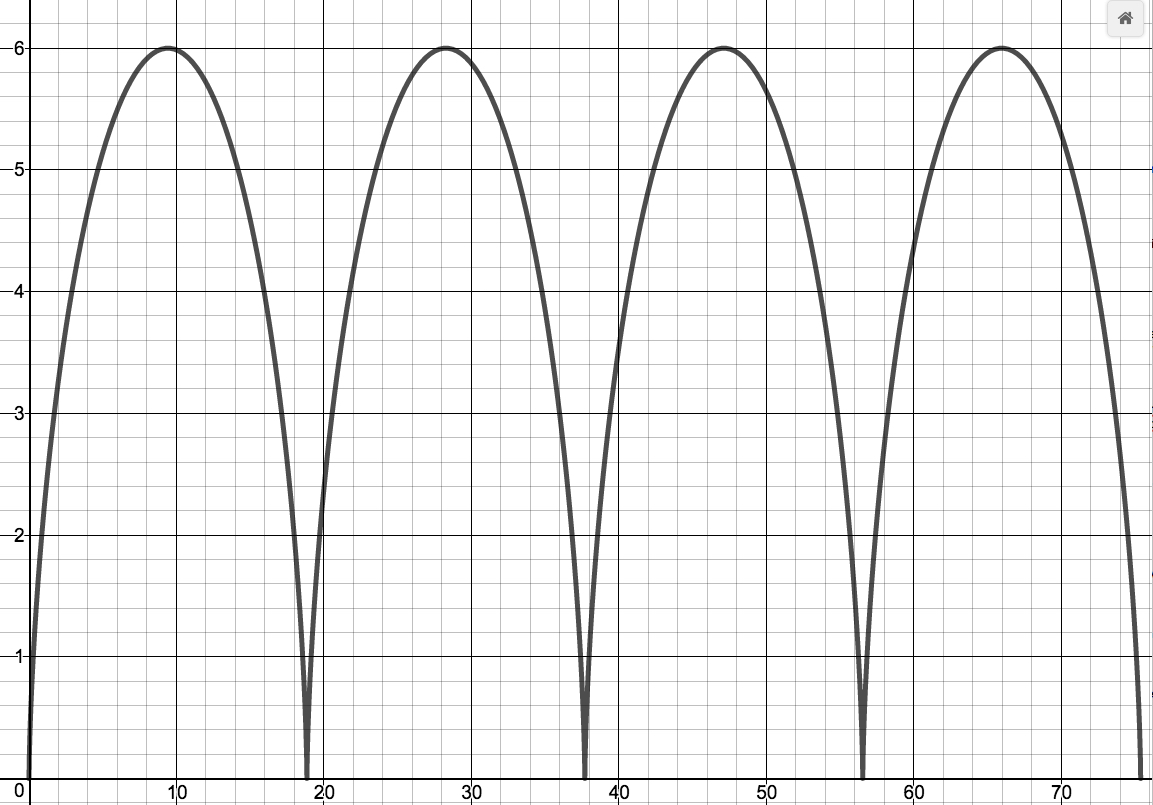
\includegraphics[width=4in]{./ParametricEquationsGraphics/cycloid.jpg}

\end{center}

We see the equations create a series of `arches' and can (partially) verify the reasonableness the graph by finding the $x$-intercepts.  To do this, we set $y = 3(1-\cos(t)) = 0$, which amounts to solving $\cos(t) = 1$.  

\smallskip

We get $t = 2 \pi k$ and since $t \geq 0$, $k$ can be any \textit{nonnegative} integer.  Substituting a few of these values for $t$, $t = 0$, $t = 2\pi$, $t = 4\pi$, and $t=6\pi$ into the equations $x = 3(t -\sin(t))$ and $y = 3(1-\cos(t))$ we obtain the points $(0,0)$, $(6\pi, 0) \approx (18.85, 0)$,  $(12 \pi,0) \approx (37.70, 0)$ and $(18\pi, 0) \approx ( 56.55 , 0)$, which match the graph. In general, the $x$-intercepts are $(6\pi k, 0)$ for nonnegative integers $k$.  We leave the details to the reader.

\smallskip

We note it is also possible to analytically determine  the (local) maximums of the graph using the techniques demonstrated in Example \ref{parametrictorect}  by analyzing $y = 3(1-\cos(t))$ .   The maximums occur when $t = (2k +1) \pi k$ where $k$ is a nonnegative integer, which isn't too surprising just looking at the problem from a  symmetry perspective.  Substituting these values for $t$ into our equations for $x$ and $y$ produce points of the form $(3(2k+1) \pi, 6)$.  We leave the details to the reader.  \qed

\end{example}



\newpage

\subsection{Exercises}


%% SKIPPED %% In Exercises \ref{paraplotfirst} - \ref{paraplotlast}, plot the set of parametric equations by hand. Be sure to indicate the orientation imparted on the curve by the parametrization.  

\begin{multicols}{2} \raggedcolumns 

\begin{enumerate}

\item ${\displaystyle \left\{ \begin{array}{l} x = 4t-3 \\ y = 6t-2 \end{array} \right. \vspace{.25in} \mbox{for } 0 \leq t \leq 1}$ \label{paraplotfirst}
\item ${\displaystyle \left\{ \begin{array}{l} x = 4t-1 \\ y = 3-4t \end{array} \right. \vspace{.25in} \mbox{for } 0 \leq t \leq 1}$

\setcounter{HW}{\value{enumi}}
\end{enumerate}
\end{multicols}

\begin{multicols}{2} \raggedcolumns 
\begin{enumerate}
\setcounter{enumi}{\value{HW}}
\item ${\displaystyle \left\{ \begin{array}{l} x = 2t \\ y = t^2 \end{array} \right. \vspace{.25in} \mbox{for } -1 \leq t \leq 2}$
\item ${\displaystyle \left\{ \begin{array}{l} x = t-1 \\ y = 3+2t-t^2 \end{array} \right. \vspace{.25in} \mbox{for } 0 \leq t \leq 3}$

\setcounter{HW}{\value{enumi}}
\end{enumerate}
\end{multicols}



\begin{multicols}{2} \raggedcolumns 
\begin{enumerate}
\setcounter{enumi}{\value{HW}}
\item ${\displaystyle \left\{ \begin{array}{l} x = t^2+2t+1 \\[3pt] y = t+1 \end{array} \right. \vspace{.25in} \mbox{for } t \leq 1}$
\item ${\displaystyle \left\{ \begin{array}{l} x = \frac{1}{9}\left(18-t^2\right) \\[3pt] y = \frac{1}{3} t \end{array} \right. \vspace{.25in} \mbox{for } t \geq -3}$

\setcounter{HW}{\value{enumi}}
\end{enumerate}
\end{multicols}


\begin{multicols}{2} \raggedcolumns 
\begin{enumerate}
\setcounter{enumi}{\value{HW}}

\item ${\displaystyle \left\{ \begin{array}{l} x = t \\ y = t^3 \end{array} \right. \vspace{.25in} \mbox{for } -\infty < t < \infty}$
\item ${\displaystyle \left\{ \begin{array}{l} x = t^3 \\ y = t \end{array} \right. \vspace{.25in} \mbox{for } -\infty < t < \infty}$

\setcounter{HW}{\value{enumi}}
\end{enumerate}
\end{multicols}

\begin{multicols}{2} \raggedcolumns 
\begin{enumerate}
\setcounter{enumi}{\value{HW}}
\item ${\displaystyle \left\{ \begin{array}{l} x = \cos(t) \\ y = \sin(t) \end{array} \right. \vspace{.25in} \mbox{for } -\dfrac{\pi}{2} \leq t \leq \dfrac{\pi}{2}}$
\item ${\displaystyle \left\{ \begin{array}{l} x = 3\cos(t) \\ y = 3\sin(t) \end{array} \right. \vspace{.25in} \mbox{for } 0 \leq t \leq \pi}$


\setcounter{HW}{\value{enumi}}
\end{enumerate}
\end{multicols}



\begin{multicols}{2} \raggedcolumns 
\begin{enumerate}
\setcounter{enumi}{\value{HW}}

\item ${\displaystyle \left\{ \begin{array}{l} x = -1+ 3\cos(t) \\ y = 4\sin(t) \end{array} \right. \vspace{.25in} \mbox{for } 0 \leq t \leq 2\pi}$
\item ${\displaystyle \left\{ \begin{array}{l} x = 3\cos(t) \\ y = 2\sin(t)+1 \end{array} \right. \vspace{.25in} \mbox{for } \dfrac{\pi}{2} \leq t \leq 2\pi}$

\setcounter{HW}{\value{enumi}}
\end{enumerate}
\end{multicols}

\begin{multicols}{2} \raggedcolumns 
\begin{enumerate}
\setcounter{enumi}{\value{HW}}

\item ${\displaystyle \left\{ \begin{array}{l} x = 2\cos(t) \\ y = \sec(t) \end{array} \right. \vspace{.25in} \mbox{for } 0 \leq t < \dfrac{\pi}{2}}$
\item ${\displaystyle \left\{ \begin{array}{l} x = 2\tan(t) \\ y = \cot(t) \end{array} \right. \vspace{.25in} \mbox{for } 0 < t < \dfrac{\pi}{2}}$

\setcounter{HW}{\value{enumi}}
\end{enumerate}
\end{multicols}


\begin{multicols}{2} \raggedcolumns 
\begin{enumerate}
\setcounter{enumi}{\value{HW}}

\item ${\displaystyle \left\{ \begin{array}{l} x = \sec(t) \\ y = \tan(t) \end{array} \right. \vspace{.25in} \mbox{for } -\dfrac{\pi}{2} < t < \dfrac{\pi}{2}}$
\item ${\displaystyle \left\{ \begin{array}{l} x = \sec(t) \\ y = \tan(t) \end{array} \right. \vspace{.25in} \mbox{for } \dfrac{\pi}{2} < t < \dfrac{3\pi}{2}}$

\setcounter{HW}{\value{enumi}}
\end{enumerate}
\end{multicols}

\begin{multicols}{2} \raggedcolumns 
\begin{enumerate}
\setcounter{enumi}{\value{HW}}

\item ${\displaystyle \left\{ \begin{array}{l} x = \tan(t) \\ y = 2\sec(t) \end{array} \right. \vspace{.25in} \mbox{for } -\dfrac{\pi}{2} < t < \dfrac{\pi}{2}}$
\item ${\displaystyle \left\{ \begin{array}{l} x = \tan(t) \\ y = 2\sec(t) \end{array} \right. \vspace{.25in} \mbox{for } \dfrac{\pi}{2} < t < \dfrac{3\pi}{2}}$

\setcounter{HW}{\value{enumi}}
\end{enumerate}
\end{multicols}


\begin{multicols}{2} \raggedcolumns 
\begin{enumerate}
\setcounter{enumi}{\value{HW}}

\item ${\displaystyle \left\{ \begin{array}{l} x = \cos(t) \\ y = t \end{array} \right. \vspace{.25in} \mbox{for } 0 \leq t \leq \pi}$
\item ${\displaystyle \left\{ \begin{array}{l} x = \sin(t) \\ y = t \end{array} \right. \vspace{.25in} \mbox{for } -\dfrac{\pi}{2} \leq t \leq \dfrac{\pi}{2}}$ \label{paraplotlast}

\setcounter{HW}{\value{enumi}}
\end{enumerate}
\end{multicols}

\newpage

In the same way (and for the same reason) we took the time on page \pageref{polargraphscalculator} in Section \ref{PolarGraphs} to show how to graph polar equations using a graphing calculator, we take a few moments here to explain how to graph a system of parametric equations using a calculator.  Our task is to graph the cycloid from Example \ref{cycloidex},  $\left\{ x = 3(t -\sin(t)), \, y = 3(1-\cos(t)) \right.$ for $t \geq 0$ using a graphing calculator.

\smallskip

We first must ensure that the calculator is in `Parametric Mode' and `radian mode' when we enter the equations and advance to the `Window' screen. 

\begin{center}

\begin{tabular}{cc}

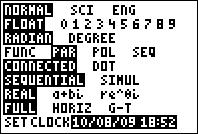
\includegraphics[width=2in]{./ParametricEquationsGraphics/Parametric01.jpg} &
\hspace{0.75in} 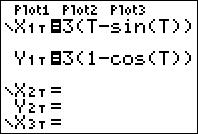
\includegraphics[width=2in]{./ParametricEquationsGraphics/Parametric02.jpg} \\

\end{tabular} 

\end{center}

Our next step is to find appropriate bounds on the parameter, $t$, as well as for $x$ and $y$.   We know that one full revolution of the circle occurs over the interval $0 \leq t < 2\pi$, so it seems reasonable to keep these as our bounds on $t$.  The `Tstep' seems reasonably small -- too large a value here can lead to incorrect graphs.\footnote{Again, see page \pageref{polargraphscalculator} in Section \ref{PolarGraphs}.}  We know from our derivation of the equations of the cycloid that the center of the generating circle has coordinates $(r\theta,r)  = (3t,3)$.  Since  $t$ ranges between $0$ and $2\pi$, we set $x$ to range between $0$ and $6\pi$.  The values of $y$ go from the bottom of the circle to the top, so $y$ ranges between $0$ and $6$.

\begin{center}
\begin{tabular}{cc}

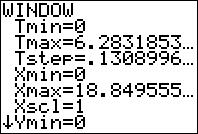
\includegraphics[width=2in]{./ParametricEquationsGraphics/Parametric03.jpg} &
\hspace{0.75in} 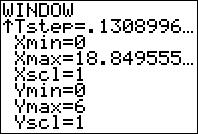
\includegraphics[width=2in]{./ParametricEquationsGraphics/Parametric04.jpg} \\

\end{tabular} 


\end{center}

Below we graph the cycloid with these settings, and then extend $t$ to range from $0$ to $6\pi$ which forces $x$ to range from $0$ to $18\pi$ yielding three arches of the cycloid.\footnote{It is instructive to note that keeping the $y$ settings between 0 and 6 skews the aspect ratio of the cycloid.  Using the `Zoom Square' feature on the graphing calculator gives a true geometric perspective of the three arches.}

\begin{center}

\begin{tabular}{cc}

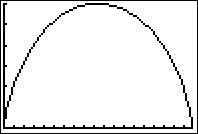
\includegraphics[width=2in]{./ParametricEquationsGraphics/Parametric05.jpg} &
\hspace{0.75in} 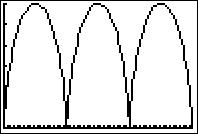
\includegraphics[width=2in]{./ParametricEquationsGraphics/Parametric06.jpg} \\


\end{tabular} 
\end{center}


In Exercises \ref{paracalcfirst} - \ref{paracalclast}, plot the set of parametric equations with the help of a graphing utility.  Be sure to indicate the orientation imparted on the curve by the parametrization.  

\begin{multicols}{2} \raggedcolumns 
\begin{enumerate}
\setcounter{enumi}{\value{HW}}


\item ${\displaystyle \left\{ \begin{array}{l} x = t^{3} - 3t \\ y = t^{2} - 4 \end{array} \right. \vspace{.25in} \mbox{for } -2 \leq t \leq 2}$ \label{paracalcfirst}
\item ${\displaystyle \left\{ \begin{array}{l} x = 4\cos^{3}(t) \\ y = 4\sin^{3}(t) \end{array} \right. \vspace{.25in} \mbox{for } 0 \leq t \leq 2\pi}$

\setcounter{HW}{\value{enumi}}
\end{enumerate}
\end{multicols}

\begin{multicols}{2} \raggedcolumns 
\begin{enumerate}
\setcounter{enumi}{\value{HW}}


\item ${\displaystyle \left\{ \begin{array}{l} x = e^{t} + e^{-t} \\ y = e^{t} - e^{-t} \end{array} \right. \vspace{.25in} \mbox{for }  -2 \leq t \leq 2}$
\item ${\displaystyle \left\{ \begin{array}{l} x = \cos(3t) \\ y = \sin(4t) \end{array} \right. \vspace{.25in} \mbox{for } 0 \leq t \leq 2\pi}$ \label{paracalclast}

\setcounter{HW}{\value{enumi}}
\end{enumerate}
\end{multicols}


In Exercises \ref{findparamfirst} - \ref{findparamlast}, find a parametric description for the given oriented curve.

\begin{enumerate}

\setcounter{enumi}{\value{HW}}

\item  the directed line segment from $(3,-5)$ to $(-2,2)$ \label{findparamfirst}

\item  the directed line segment from $(-2,-1)$ to $(3, -4)$ 

\item  the curve $y = 4-x^2$ from $(-2,0)$ to $(2,0)$.

\item   the curve $y = 4-x^2$ from $(-2,0)$ to $(2,0)$ \\
(Shift the parameter so  $t=0$ corresponds to $(-2,0)$.)

\item  the curve $x = y^2 - 9$ from $(-5,-2)$ to $(0,3)$.

\item  the curve $x = y^2 - 9$ from $(0,3)$ to $(-5,-2)$.\\
(Shift the parameter so  $t=0$ corresponds to $(0,3)$.)

\item   the circle $x^2 + y^2 = 25$, oriented counter-clockwise

\item   the circle $(x-1)^2 + y^2 = 4$, oriented counter-clockwise

\item   the circle $x^2 + y^2 - 6y = 0$, oriented counter-clockwise

\item   the circle $x^2 + y^2 - 6y = 0$, oriented \emph{clockwise}\\
(Shift the parameter so  $t$ begins at $0$.)

\item   the circle $(x-3)^2 + (y+1)^2 = 117$, oriented counter-clockwise

\item   the ellipse $(x-1)^2 + 9y^2 = 9$, oriented counter-clockwise

\item   the ellipse $9x^2 + 4y^2 + 24y =0$, oriented counter-clockwise

\item   the ellipse $9x^2 + 4y^2 + 24y =0$, oriented clockwise  \\
(Shift the parameter so $t=0$ corresponds to  $(0,0)$.)

\item  the triangle with vertices $(0,0)$, $(3,0)$, $(0,4)$, oriented counter-clockwise \\
(Shift the parameter so $t=0$ corresponds to $(0,0)$.) \label{findparamlast}

\setcounter{HW}{\value{enumi}}

\end{enumerate}

\begin{enumerate}

\setcounter{enumi}{\value{HW}}

\item Use parametric equations and a graphing utility to graph the inverse of $f(x) = x^{3} + 3x - 4$.

\item  Every polar curve $r = f(\theta)$ can be translated to a system of parametric equations with parameter $\theta$ by $\left\{ x = r\cos(\theta) = f(\theta) \cos(\theta), \, y = r \sin(\theta) = f(\theta) \sin(\theta) \right.$.  Convert $r = 6\cos(2\theta)$ to a system of parametric equations. Check your answer by graphing $r = 6\cos(2\theta)$ by hand using the techniques presented in Section \ref{PolarGraphs} and then graphing the parametric equations you found using a graphing utility.


\item  Use your results from Exercises \ref{heightlondoneye} and \ref{leftrightlondoneye} in Section \ref{Sinusoid} to find the parametric equations which model a passenger's position as they ride the \href{http://en.wikipedia.org/wiki/London_Eye}{\underline{London Eye}}. 




\setcounter{HW}{\value{enumi}}
\end{enumerate}

\phantomsection
\label{projectoilemotion}

Suppose an object, called a projectile, is launched into the air.  Ignoring everything except the force gravity, the path of the projectile is given by\footnote{A nice mix of vectors and Calculus are needed to derive this.}

\[ \left\{ \begin{array}{l} x =   v_{\text{\tiny $0$}} \cos(\theta) \, t \\ [3pt]
															y = -\dfrac{1}{2} g t^2 +  v_{\text{\tiny $0$}} \sin(\theta) \, t + s_{\text{\tiny $0$}} \\ \end{array} \right. \; \text{for} \; 0 \leq t \leq T \]

where  $v_{\text{\tiny $0$}}$ is the initial speed of the object, $\theta$ is the angle from the horizontal at which the projectile is launched,\footnote{We've seen this before.  It's the angle of elevation which was defined on page \pageref{angleofelevation}.} $g$ is the acceleration due to gravity,  $s_{\text{\tiny $0$}}$ is the initial height of the projectile above the ground and $T$ is the time when the object returns to the ground.  (See the figure below.)

\begin{center}

\begin{mfpic}[20]{-1}{9}{-1}{7}
\axes
\tlabel[cc](9,-0.5){\scriptsize $x$}
\tlabel[cc](0.5,7){\scriptsize $y$}
\dashed \polyline{(0,4), (1.5,4)}
\tlabelsep{5pt}
\axislabels{y}{{\scriptsize $s_{\text{\tiny $0$}}$} 4}
\point[4pt]{(0,4), (5.98,0)}
\arrow \shiftpath{(0,4)}  \parafcn{5, 55, 5}{0.75*dir(t)}
\tlabel[cc](1,4.5){\scriptsize $\theta$}
\tlabel[cc](5.98,-0.5){\scriptsize $(x(T), 0)$}
\penwd{1.25pt}
\arrow \parafcn{0,0.75,0.1}{(3.5*t, 6.062*t+4-(4.9*(t**2)))}
\parafcn{0.75,1.71,0.1}{(3.5*t, 6.062*t+4-(4.9*(t**2)))}

\end{mfpic}


\end{center}

\begin{enumerate}
\setcounter{enumi}{\value{HW}}

\item  Carl's friend Jason competes in Highland Games Competitions across the country.  In one event, the `hammer throw',  he throws a 56 pound weight for distance. If the weight is released $6$ feet above the ground at an angle of $42^{\circ}$ with respect to the horizontal with an initial speed of $33$ feet per second, find the parametric equations for the flight of the hammer.  (Here, use $g = 32 \frac{\text{ft.}}{s^2}$.) When will the hammer hit the ground?  How far away will it hit the ground? Check your answer using a graphing utility.

\item  \label{projectileeliminate} Eliminate the parameter in the equations for projectile motion to show that the path of the projectile follows the curve \[y = -\dfrac{g \sec^{2}(\theta)}{2 v_{\text{\tiny$0$}}^2} x^2 + \tan(\theta) x + s_{\text{\tiny $0$}}\] Use the vertex formula (Equation \ref{vertexofquadraticfunctions}) to show the maximum height of the projectile is \[y = \dfrac{v_{\text{\tiny$0$}}^2 \sin^{2}(\theta)}{2g} + s_{\text{\tiny $0$}} \quad \text{when} \quad x = \dfrac{v_{\text{\tiny$0$}}^2 \sin(2\theta) }{2g}\] 

\item  In another event, the `sheaf toss', Jason throws a  20 pound weight for height.  If the weight is released  5 feet above the ground at an angle of $85^{\circ}$ with respect to the horizontal and the sheaf reaches a maximum height of 31.5 feet, use your results from part  \ref{projectileeliminate} to determine how fast the sheaf was launched into the air.  (Once again, use $g = 32 \frac{\text{ft.}}{s^2}$.)

\item  Suppose $\theta = \frac{\pi}{2}$. (The projectile was launched vertically.) Simplify the general parametric formula given for $y(t)$ above using  $g = 9.8 \, \frac{m}{s^2}$ and compare that to the formula for $s(t)$ given in Exercise \ref{whatgoesup} in Section \ref{QuadraticFunctions}.  What is $x(t)$ in this case?

\item  If $f$ and $g$ are functions, explain why the function $\vec{r}(t) = \left<f(t), g(t) \right>$ is a function. The function $\vec{r}$ is called a \index{function ! vector-valued}\index{vector-valued function}\textbf{vector-valued function} since it matches real number inputs, $t$, with vector outputs, $\vec{r}(t)$.   Explain why when the vectors  $\vec{r}(t)$ are plotted in standard position, their terminal points trace out the curve described parametrically by the system of equations:  $\left\{ x = f(t) \, y =  g(t) \right.$  (In Calculus, you will see  systems of parametric equations `packaged' together using vectors.)

\setcounter{HW}{\value{enumi}}
\end{enumerate}


\phantomsection
\label{hyperboliccosinesine} 

In Exercises \ref{hyperbolicfirst} - \ref{hyperboliclast}, we explore the  \textbf{hyperbolic cosine}\index{hyperbolic cosine} function, denoted $\cosh(t)$, and the \textbf{hyperbolic sine}\index{hyperbolic sine}
function, denoted $\sinh(t)$, defined below:

\[ \begin{array}{ccc}

\cosh(t) = \dfrac{e^{t} + e^{-t}}{2} & 
\text{and} & \sinh(t) = \dfrac{e^{t} - e^{-t}}{2} \\

\end{array} \]

\begin{enumerate}
\setcounter{enumi}{\value{HW}}

\item  Using a graphing utility as needed, verify the following:  \label{hyperbolicfirst}

\begin{enumerate}

\item the domain of $\cosh(t)$ is $(-\infty, \infty)$ and the range of $\cosh(t)$ is $[1,\infty)$.

\item  the domain and range  of $\sinh(t)$ are both $(-\infty, \infty)$.

\end{enumerate}

\item  Show that $\left\{ x(t) = \cosh(t), \, y(t) = \sinh(t) \right.$ parametrize the right half of the `unit' hyperbola $x^2 - y^2 = 1$.  (Hence the use of the adjective `hyperbolic.')

\item  Compare and contrast the definitions of $\cosh(t)$ and $\sinh(t)$ to the formulas for $\cos(t)$ and $\sin(t)$ given in Exercise \ref{expformcosandsin} in Section \ref{PolarComplex}.

\item \label{andtheresthyperbolic} Four other hyperbolic functions are waiting to be defined:  the hyperbolic secant $\text{sech}(t)$, the hyperbolic cosecant $\text{csch}(t)$, the hyperbolic tangent $\tanh(t)$ and the hyperbolic cotangent $\coth(t)$.  Define these functions in terms of $\cosh(t)$ and $\sinh(t)$, then convert them to formulas involving $e^{t}$ and $e^{-t}$.  Consult a suitable reference (a Calculus book, or this entry on the \href{http://en.wikipedia.org/wiki/Hyperbolic_function}{\underline{hyperbolic functions}}) and spend some time reliving the thrills of trigonometry with these `hyperbolic' functions.

\item  If these functions look familiar, they should.  Enjoy some nostalgia and revisit Exercise \ref{catenary} in Section \ref{ExpLogApplications}, Exercise \ref{hyperbolicsine} in Section \ref{ExponentialEquationsandInequalities} and the  answer to Exercise \ref{inversehyptangent} in Section \ref{LogarithmicEquationsandInequalities}. \label{hyperboliclast}

\end{enumerate}

\newpage

\subsection{Answers}

\begin{multicols}{2} \raggedcolumns 
\begin{enumerate}

\item ${\displaystyle \left\{ \begin{array}{l} x = 4t-3 \\ y = 6t-2 \end{array} \right. \vspace{.25in} \mbox{for } 0 \leq t \leq 1}$

\begin{mfpic}[15]{-4}{2}{-3}{5}
\axes
\tlabel[cc](2,-0.5){\scriptsize $x$}
\tlabel[cc](0.5,5){\scriptsize $y$}
\xmarks{-3,-2,-1,1}
\ymarks{-2,-1,1,2,3,4}
\point[4pt]{(-3,-2), (1,4)}
\tlpointsep{4pt}
\scriptsize
\axislabels {x}{{$-3 \hspace{6pt}$} -3,{$-2 \hspace{6pt}$} -2,{$-1 \hspace{6pt}$} -1, {$1$} 1}
\axislabels {y}{{$-1$} -1,{$-2$} -2, {$1$} 1,{$2$} 2,{$3$} 3,{$4$} 4}
\normalsize
\penwd{1.25pt}
\arrow \parafcn{0,0.5,0.1}{(4*t-3,6*t-2)}
\parafcn{0.5,1,0.1}{(4*t-3,6*t-2)}
\end{mfpic}


\item ${\displaystyle \left\{ \begin{array}{l} x = 4t-1 \\ y = 3-4t \end{array} \right. \vspace{.25in} \mbox{for } 0 \leq t \leq 1}$


\begin{mfpic}[15]{-2}{4}{-2}{4}
\axes
\tlabel[cc](4,-0.5){\scriptsize $x$}
\tlabel[cc](0.5,4){\scriptsize $y$}
\xmarks{-1,1,2,3}
\ymarks{-1,1,2,3}
\point[4pt]{(-1,3), (3,-1)}
\tlpointsep{4pt}
\scriptsize
\axislabels {x}{{$-1 \hspace{6pt}$} -1, {$1$} 1, {$2$} 2,{$3$} 3}
\axislabels {y}{{$-1$} -1, {$1$} 1,{$2$} 2,{$3$} 3}
\normalsize
\penwd{1.25pt}
\arrow \parafcn{0,0.5,0.1}{(4*t-1,3-4*t)}
\parafcn{0.5,1,0.1}{(4*t-1,3-4*t)}
\end{mfpic}
\setcounter{HW}{\value{enumi}}
\end{enumerate}
\end{multicols}



\begin{multicols}{2} \raggedcolumns 
\begin{enumerate}
\setcounter{enumi}{\value{HW}}

\item ${\displaystyle \left\{ \begin{array}{l} x = 2t \\ y = t^2 \end{array} \right. \vspace{.25in} \mbox{for } -1 \leq t \leq 2}$

\begin{mfpic}[15]{-3}{5}{-1}{5}
\axes
\tlabel[cc](5,-0.5){\scriptsize $x$}
\tlabel[cc](0.5,5){\scriptsize $y$}
\xmarks{-2,-1,1,2,3,4}
\ymarks{1,2,3,4}
\point[4pt]{(-2,1), (0,0), (4,4)}
\tlpointsep{4pt}
\scriptsize
\axislabels {x}{{$-3 \hspace{6pt}$} -3,{$-2 \hspace{6pt}$} -2,{$-1 \hspace{6pt}$} -1, {$1$} 1, {$2$} 2,{$3$} 3,{$4$} 4}
\axislabels {y}{{$1$} 1,{$2$} 2,{$3$} 3,{$4$} 4}
\normalsize
\penwd{1.25pt}
\arrow \parafcn{-1,-0.5,0.1}{(2*t,(t**2))}
\arrow \parafcn{-0.5,1,0.1}{(2*t,(t**2))}
\parafcn{1,2,0.1}{(2t,t**2)}
\end{mfpic}


\item ${\displaystyle \left\{ \begin{array}{l} x = t-1 \\ y = 3+2t-t^2 \end{array} \right. \vspace{.25in} \mbox{for } 0 \leq t \leq 3}$


\begin{mfpic}[15]{-2}{3}{-1}{5}
\axes
\tlabel[cc](4,-0.5){\scriptsize $x$}
\tlabel[cc](0.5,5){\scriptsize $y$}
\xmarks{-1,1,2}
\ymarks{1,2,3,4}
\point[4pt]{(-1,3), (0,4), (2,0)}
\tlpointsep{4pt}
\scriptsize
\axislabels {x}{{$-1 \hspace{6pt}$} -1, {$1$} 1, {$2$} 2}
\axislabels {y}{{$1$} 1,{$2$} 2,{$3$} 3,{$4$} 4}
\normalsize
\penwd{1.25pt}
\arrow \parafcn{0,0.5,0.1}{(t-1,3+2*t-(t**2))}
\arrow \parafcn{0.5,2,0.1}{(t-1,3+2*t-(t**2))}
\parafcn{2,3,0.1}{(t-1,3+2*t-(t**2))}

\end{mfpic}

\setcounter{HW}{\value{enumi}}
\end{enumerate}
\end{multicols}


\begin{multicols}{2} \raggedcolumns 
\begin{enumerate}
\setcounter{enumi}{\value{HW}}

\item ${\displaystyle \left\{ \begin{array}{l} x = t^2+2t+1 \\ y = t+1 \end{array} \right. \vspace{.25in} \mbox{for } t \leq 1}$

\begin{mfpic}[15]{-1}{6}{-3}{3}
\axes
\tlabel[cc](6,-0.5){\scriptsize $x$}
\tlabel[cc](0.5,3){\scriptsize $y$}
\xmarks{1,2,3,4,5}
\ymarks{-2,-1,1,2}
\point[4pt]{(4,2), (0,0), (4,-2)}
\tlpointsep{4pt}
\scriptsize
\axislabels {x}{ {$1$} 1, {$2$} 2,{$3$} 3,{$4$} 4,{$5$} 5}
\axislabels {y}{{$-2$} -2,{$-1$} -1,{$1$} 1,{$2$} 2,{$3$}}
\normalsize
\penwd{1.25pt}
\parafcn{0,1,0.1}{((t**2)+(2*t)+1,t+1)}
\arrow \parafcn{-2,0,0.1}{((t**2)+(2*t)+1,t+1)}
\arrow \parafcn{-3.25,-2,0.1}{((t**2)+(2*t)+1,t+1)}
\arrow \parafcn{-3.44,-3.25,0.1}{((t**2)+(2*t)+1,t+1)}
\end{mfpic} 

\item ${\displaystyle \left\{ \begin{array}{l} x = \frac{1}{9}\left(18-t^2\right) \\ y = \frac{1}{3} t \end{array} \right. \vspace{.25in} \mbox{for } t \geq -3}$



\begin{mfpic}[15]{-4}{3}{-2}{3}
\axes
\tlabel[cc](3,-0.5){\scriptsize $x$}
\tlabel[cc](0.5,3){\scriptsize $y$}
\xmarks{-3,-2,-1,1,2}
\ymarks{-1,1,2}
\point[4pt]{(1,-1), (2,0), (-2,2)}
\tlpointsep{4pt}
\scriptsize
\axislabels {x}{{$-3 \hspace{6pt}$} -3,{$-2 \hspace{6pt}$} -2,{$-1 \hspace{6pt}$} -1, {$1$} 1, {$2$} 2}
\axislabels {y}{{$-1$} -1,{$1$} 1,{$2$} 2}
\normalsize
\penwd{1.25pt}
\arrow \parafcn{-3,-1.5,0.1}{((18-(t**2))/9,t/3)}
\arrow \parafcn{-1.5,3,0.1}{((18-(t**2))/9,t/3)}
\arrow \parafcn{3,6.5,0.1}{((18-(t**2))/9,t/3)}

\end{mfpic}

\setcounter{HW}{\value{enumi}}
\end{enumerate}
\end{multicols}


\pagebreak


\begin{multicols}{2} \raggedcolumns 
\begin{enumerate}
\setcounter{enumi}{\value{HW}}

\item ${\displaystyle \left\{ \begin{array}{l} x = t \\ y = t^3 \end{array} \right. \vspace{.25in} \mbox{for } -\infty < t < \infty}$


\begin{mfpic}[15]{-2}{2}{-5}{5}
\axes
\tlabel[cc](2,-0.5){\scriptsize $x$}
\tlabel[cc](0.5,5){\scriptsize $y$}
\xmarks{-1,1}
\ymarks{-4,-3,-2,-1,1,2,3,4}
\point[4pt]{(-1,-1), (0,0), (1,1)}
\tlpointsep{4pt}
\scriptsize
\axislabels {x}{{$-1 \hspace{6pt}$} -1, {$1$} 1}
\axislabels {y}{{$-4$} -4,{$-3$} -3,{$-2$} -2,{$-1$} -1,{$1$} 1,{$2$} 2,{$3$} 3,{$4$} 4}
\normalsize
\penwd{1.25pt}
\arrow \parafcn{-1.7,-1.25,0.1}{(t, t**3)}
\arrow \parafcn{-1.25,1.25,0.1}{(t, t**3)}
\arrow \parafcn{1.25,1.7,0.1}{(t, t**3)}
\end{mfpic}


\item ${\displaystyle \left\{ \begin{array}{l} x = t^3 \\ y = t \end{array} \right. \vspace{.25in} \mbox{for } -\infty < t < \infty}$

\begin{mfpic}[15]{-5}{5}{-2}{2}
\axes
\tlabel[cc](5,-0.5){\scriptsize $x$}
\tlabel[cc](0.5,2){\scriptsize $y$}
\xmarks{-4,-3,-2,-1,1,2,3,4}
\ymarks{-1,1}
\point[4pt]{(-1,-1), (0,0), (1,1)}
\tlpointsep{4pt}
\scriptsize
\axislabels {y}{{$-1$} -1, {$1$} 1}
\axislabels {x}{{$-4 \hspace{6pt}$} -4,{$-3 \hspace{6pt}$} -3,{$-2 \hspace{6pt}$} -2,{$-1 \hspace{6pt}$} -1,{$1$} 1,{$2$} 2,{$3$} 3,{$4$} 4}
\normalsize
\penwd{1.25pt}
\arrow \parafcn{-1.7,-1.25,0.1}{(t**3, t)}
\arrow \parafcn{-1.25,1.25,0.1}{(t**3, t)}
\arrow \parafcn{1.25,1.7,0.1}{(t**3, t)}
\end{mfpic}


\setcounter{HW}{\value{enumi}}
\end{enumerate}
\end{multicols}



\begin{multicols}{2}

\begin{enumerate}

\setcounter{enumi}{\value{HW}}
\item ${\displaystyle \left\{ \begin{array}{l} x = \cos(t) \\ y = \sin(t) \end{array} \right. \vspace{.25in} \mbox{for } -\dfrac{\pi}{2} \leq t \leq \dfrac{\pi}{2}}$

\begin{mfpic}[10]{-5}{5}{-5}{5}
\axes
\tlabel[cc](5,-0.5){\scriptsize $x$}
\tlabel[cc](0.5,5){\scriptsize $y$}
\point[4pt]{(0,-4), (4,0), (0,4)}
\xmarks{-4,4}
\ymarks{-4,4}
\tlpointsep{4pt}
\scriptsize
\axislabels {x}{{$-1 \hspace{6pt}$} -4, {$1$} 4}
\axislabels {y}{{$-1$} -4, {$1$} 4}
\normalsize
\penwd{1.25pt}
\arrow \parafcn{-1.57,-0.78,0.1}{(4*cos(t),4*sin(t))}
\arrow \parafcn{-0.78,0.78,0.1}{(4*cos(t),4*sin(t))}
\parafcn{0.78,1.57,0.1}{(4*cos(t),4*sin(t))}
\end{mfpic} 


\item ${\displaystyle \left\{ \begin{array}{l} x = 3\cos(t) \\ y = 3\sin(t) \end{array} \right. \vspace{.25in} \mbox{for } 0 \leq t \leq \pi}$

\begin{mfpic}[15]{-4}{4}{-1}{4}
\axes
\tlabel[cc](4,-0.5){\scriptsize $x$}
\tlabel[cc](0.5,4){\scriptsize $y$}
\point[4pt]{(-3,0), (3,0), (0,3)}
\xmarks{-3,-2,-1,1,2,3}
\ymarks{1,2,3}
\tlpointsep{4pt}
\scriptsize
\axislabels {x}{{$-3 \hspace{6pt}$} -3, {$-2 \hspace{6pt}$} -2,{$-1 \hspace{6pt}$} -1,{$1$} 1,{$2$} 2,{$3$} 3}
\axislabels {y}{{$1$} 1,{$2$} 2,{$3$} 3}
\normalsize
\penwd{1.25pt}
\arrow \parafcn{0,0.78,0.1}{(3*cos(t),3*sin(t))}
\arrow \parafcn{0.78,2.36,0.1}{(3*cos(t),3*sin(t))}
\parafcn{2.36,3.14,0.1}{(3*cos(t),3*sin(t))}
\end{mfpic} 

\setcounter{HW}{\value{enumi}}
\end{enumerate}
\end{multicols}




\begin{multicols}{2}
\begin{enumerate}
\setcounter{enumi}{\value{HW}}

\item  ${\displaystyle \left\{ \begin{array}{l} x = -1+3\cos(t) \\ y = 4\sin(t) \end{array} \right. \vspace{.25in} \mbox{for } 0 \leq t \leq 2\pi}$

\begin{mfpic}[15]{-5}{3}{-5}{5}
\axes
\tlabel[cc](3,-0.5){\scriptsize $x$}
\tlabel[cc](0.5,5){\scriptsize $y$}
\point[4pt]{(2,0), (-1,4), (-4,0), (-1,-4)}
\xmarks{-4,-3,-2,-1,1,2}
\ymarks{-4,-3,-2,-1,1,2,3,4}
\tlpointsep{4pt}
\scriptsize
\axislabels {x}{{$-4 \hspace{6pt}$} -4,{$-3 \hspace{6pt}$} -3,{$-2 \hspace{6pt}$} -2, {$-1 \hspace{6pt}$} -1,{$1$} 1,{$2$} 2}
\axislabels {y}{{$-4$} -4, {$-3$} -3,{$-2$} -2,{$-1$} -1,{$1$} 1,{$2$} 2,{$3$} 3,{$4$} 4}
\normalsize
\penwd{1.25pt}
\arrow \parafcn{0,0.78,0.1}{(3*cos(t)-1,4*sin(t))}
\arrow \parafcn{0.78,2.36, 0.1}{(3*cos(t)-1,4*sin(t))}
\arrow \parafcn{2.36,3.93, 0.1}{(3*cos(t)-1,4*sin(t))}
\arrow \parafcn{3.93,5.5, 0.1}{(3*cos(t)-1,4*sin(t))}
\parafcn{5.5,6.28, 0.1}{(3*cos(t)-1,4*sin(t))}
\end{mfpic} 

\item ${\displaystyle \left\{ \begin{array}{l} x = 3\cos(t) \\ y = 2\sin(t)+1 \end{array} \right. \vspace{.25in} \mbox{for } \dfrac{\pi}{2} \leq t \leq 2\pi}$

\begin{mfpic}[15]{-4}{4}{-2}{4}
\axes
\tlabel[cc](4,-0.5){\scriptsize $x$}
\tlabel[cc](0.5,4){\scriptsize $y$}
\point[4pt]{(0,3), (-3,1), (0,-1), (3,1)}
\xmarks{-3,-2,-1,1,2,3}
\ymarks{-1,1,2,3}
\tlpointsep{4pt}
\scriptsize
\axislabels {x}{{$-3 \hspace{6pt}$} -3, {$-1 \hspace{6pt}$} -1,{$1$} 1,{$3$} 3}
\axislabels {y}{{$-1$} -1,{$1$} 1,{$2$} 2,{$3$} 3}
\normalsize
\penwd{1.25pt}
\arrow \parafcn{1.57,2.36,0.1}{(3*cos(t),1+2*sin(t))}
\arrow \parafcn{2.36,3.93,0.1}{(3*cos(t),1+2*sin(t))}
\arrow \parafcn{3.93,5.50,0.1}{(3*cos(t),1+2*sin(t))}
\parafcn{5.50,6.28,0.1}{(3*cos(t),1+2*sin(t))}
\end{mfpic} 

\setcounter{HW}{\value{enumi}}
\end{enumerate}
\end{multicols}

\begin{multicols}{2} \raggedcolumns 
\begin{enumerate}
\setcounter{enumi}{\value{HW}}

\item ${\displaystyle \left\{ \begin{array}{l} x = 2\cos(t) \\ y = \sec(t) \end{array} \right. \vspace{.25in} \mbox{for } 0 \leq t < \dfrac{\pi}{2}}$


\begin{mfpic}[25]{-1}{5}{-1}{5}
\axes
\tlabel[cc](5,-0.5){\scriptsize $x$}
\tlabel[cc](0.5,5){\scriptsize $y$}
\point[4pt]{(2,1)}
\xmarks{1,2,3,4}
\ymarks{1,2,3,4}
\tlpointsep{4pt}
\scriptsize
\axislabels {x}{{$1$} 1,{$2$} 2,{$3$} 3,{$4$} 4}
\axislabels {y}{{$1$} 1,{$2$} 2,{$3$} 3,{$4$} 4}
\normalsize
\penwd{1.25pt}
\arrow \parafcn{0,1,0.1}{(2*cos(t),sec(t))}
\arrow \parafcn{1,1.31,0.1}{(2*cos(t),sec(t))}
\end{mfpic} 


\item ${\displaystyle \left\{ \begin{array}{l} x = 2\tan(t) \\ y = \cot(t) \end{array} \right. \vspace{.25in} \mbox{for } 0 < t < \dfrac{\pi}{2}}$

\begin{mfpic}[25]{-1}{5}{-1}{5}
\axes
\tlabel[cc](5,-0.5){\scriptsize $x$}
\tlabel[cc](0.5,5){\scriptsize $y$}

\xmarks{1,2,3,4}
\ymarks{1,2,3,4}
\tlpointsep{4pt}
\scriptsize
\axislabels {x}{{$1$} 1,{$2$} 2,{$3$} 3,{$4$} 4}
\axislabels {y}{{$1$} 1,{$2$} 2,{$3$} 3,{$4$} 4}
\normalsize
\penwd{1.25pt}
\arrow \parafcn{0.25,0.4,0.1}{(2*tan(t),cot(t))}
\arrow \parafcn{0.4,0.7,0.1}{(2*tan(t),cot(t))}
\arrow \parafcn{0.7,1.1,0.1}{(2*tan(t),cot(t))}
\end{mfpic} 

\setcounter{HW}{\value{enumi}}
\end{enumerate}
\end{multicols}





\begin{multicols}{2}
\begin{enumerate}
\setcounter{enumi}{\value{HW}}

\item ${\displaystyle \left\{ \begin{array}{l} x = \sec(t) \\ y = \tan(t) \end{array} \right. \vspace{.25in} \mbox{for } -\dfrac{\pi}{2} < t < \dfrac{\pi}{2}}$

\begin{mfpic}[15]{-1}{5}{-5}{5}
\axes
\tlabel[cc](5,-0.5){\scriptsize $x$}
\tlabel[cc](0.5,5){\scriptsize $y$}
\point[4pt]{(1,0)}
\xmarks{1,2,3,4}
\ymarks{-4,-3,-2,-1,1,2,3,4}
\tlpointsep{4pt}
\scriptsize
\axislabels {x}{{$1$} 1,{$2$} 2,{$3$} 3,{$4$} 4}
\axislabels {y}{{$-4$} -4, {$-3$} -3,{$-2$} -2,{$-1$} -1,{$1$} 1,{$2$} 2,{$3$} 3,{$4$} 4}
\normalsize
\dashed \polyline{(4,4),(-1,-1)}
\dashed \polyline{(4,-4),(-1,1)}
\penwd{1.25pt}
\arrow \parafcn{1.85,2,0.1}{(0-sec(t),tan(t))}
\arrow \parafcn{2,4.25,0.1}{(0-sec(t),tan(t))}
\arrow \parafcn{4.25,4.4,0.1}{(0-sec(t),tan(t))}

\end{mfpic} 

\item ${\displaystyle \left\{ \begin{array}{l} x = \sec(t) \\ y = \tan(t) \end{array} \right. \vspace{.25in} \mbox{for } \dfrac{\pi}{2} < t < \dfrac{3\pi}{2}}$

\begin{mfpic}[15]{-5}{1}{-5}{5}
\axes
\tlabel[cc](1,-0.5){\scriptsize $x$}
\tlabel[cc](0.5,5){\scriptsize $y$}
\point[4pt]{(-1,0)}
\xmarks{-4,-3,-2,-1}
\ymarks{-4,-3,-2,-1,1,2,3,4}
\tlpointsep{4pt}
\scriptsize
\axislabels {x}{{$-4 \hspace{6pt}$} -4,{$-3 \hspace{6pt}$} -3,{$-2 \hspace{6pt}$} -2, {$-1 \hspace{6pt}$} -1}
\axislabels {y}{{$-4$} -4, {$-3$} -3,{$-2$} -2,{$-1$} -1,{$1$} 1,{$2$} 2,{$3$} 3,{$4$} 4}
\normalsize
\dashed \polyline{(-4,4),(1,-1)}
\dashed \polyline{(-4,-4),(1,1)}
\penwd{1.25pt}
\arrow \parafcn{1.85,2,0.1}{(sec(t),tan(t))}
\arrow \parafcn{2,4.25,0.1}{(sec(t),tan(t))}
\arrow \parafcn{4.25,4.4,0.1}{(sec(t),tan(t))}

\end{mfpic} 

\setcounter{HW}{\value{enumi}}
\end{enumerate}

\end{multicols}


\pagebreak

\begin{multicols}{2}
\begin{enumerate}
\setcounter{enumi}{\value{HW}}

\item ${\displaystyle \left\{ \begin{array}{l} x = \tan(t) \\ y = 2\sec(t) \end{array} \right. \vspace{.25in} \mbox{for } -\dfrac{\pi}{2} < t < \dfrac{\pi}{2}}$

\begin{mfpic}[25]{-3}{3}{-1}{5}
\axes
\tlabel[cc](3,-0.5){\scriptsize $x$}
\tlabel[cc](0.5,5){\scriptsize $y$}
\point[4pt]{(0,2)}
\xmarks{-2,-1,1,2}
\ymarks{1,2,3,4}
\tlpointsep{4pt}
\scriptsize
\axislabels {x}{{$-2 \hspace{6pt}$} -2,{$-1 \hspace{6pt}$} -1, {$1$} 1,{$2$} 2}
\axislabels {y}{{$1$} 1,{$2$} 2,{$3$} 3,{$4$} 4}
\normalsize
\dashed \polyline{(-0.5,-1),(2,4)}
\dashed \polyline{(0.5,-1),(-2,4)}
\penwd{1.25pt}
\arrow \parafcn{-1,-0.75,0.1}{(tan(t),2*sec(t))}
\arrow \parafcn{-0.75,1,0.1}{(tan(t),2*sec(t))}
\end{mfpic} 

\item ${\displaystyle \left\{ \begin{array}{l} x = \tan(t) \\ y = 2\sec(t) \end{array} \right. \vspace{.25in} \mbox{for } \dfrac{\pi}{2} < t < \dfrac{3\pi}{2}}$


\begin{mfpic}[25]{-3}{3}{-5}{1}
\axes
\tlabel[cc](3,-0.5){\scriptsize $x$}
\tlabel[cc](0.5,1){\scriptsize $y$}
\point[4pt]{(0,-2)}
\xmarks{-2,-1,1,2}
\ymarks{-1,-2,-3,-4}
\tlpointsep{4pt}
\scriptsize
\axislabels {x}{{$-2 \hspace{6pt}$} -2,{$-1 \hspace{6pt}$} -1, {$1$} 1,{$2$} 2}
\axislabels {y}{{$-1$} -1,{$-2$} -2,{$-3$} -3,{$-4$} -4}
\normalsize
\dashed \polyline{(-0.5,1),(2,-4)}
\dashed \polyline{(0.5,1),(-2,-4)}
\penwd{1.25pt}
\arrow \parafcn{-1,-0.75,0.1}{(tan(t),0-2*sec(t))}
\arrow \parafcn{-0.75,1,0.1}{(tan(t),0-2*sec(t))}
\end{mfpic} 
\setcounter{HW}{\value{enumi}}
\end{enumerate}

\end{multicols}

\begin{multicols}{2} \raggedcolumns 
\begin{enumerate}
\setcounter{enumi}{\value{HW}}

\item ${\displaystyle \left\{ \begin{array}{l} x = \cos(t) \\ y = t \end{array} \right. \vspace{.25in} \mbox{for } 0 < t < \pi}$

\begin{mfpic}[25]{-2.25}{2.25}{-0.5}{4}
\point[4pt]{(1,0), (0,1.5708), (-1,3.1416)}
\axes
\tlabel[cc](2.25,-0.25){\scriptsize $x$}
\tlabel[cc](0.25,4){\scriptsize $y$}

\xmarks{-1,1}
\ymarks{1.5708, 3.1416}
\tlpointsep{4pt}
\axislabels {y}{{\scriptsize $\frac{\pi}{2}$} 1.5708,  {\scriptsize $\pi$} 3.1416}
\axislabels {x}{{\scriptsize $-1 \hspace{7pt}$} -1, {\scriptsize $1$} 1}
\penwd{1.25pt}
\arrow \parafcn{0, 0.78, 0.1}{(cos(t), t)}
\arrow \parafcn{0.78, 2.36, 0.1}{(cos(t), t)}
\parafcn{2.36, 3.14, 0.1}{(cos(t), t)}

\end{mfpic}


\item ${\displaystyle \left\{ \begin{array}{l} x = \sin(t) \\ y = t \end{array} \right. \vspace{.25in} \mbox{for } -\dfrac{\pi}{2} < t < \dfrac{\pi}{2}}$

\begin{mfpic}[25]{-2}{2}{-2}{2}
\point[4pt]{(-1,-1.5708), (0,0), (1,1.5708)}
\axes
\tlabel[cc](2,-0.25){\scriptsize $x$}
\tlabel[cc](0.25,2){\scriptsize $y$}
\ymarks{-1.5708, 1.5708}
\xmarks{-1,1}
\tlpointsep{4pt}
\axislabels {y}{{\scriptsize $-\frac{\pi}{2}$} -1.5708, {\scriptsize $\frac{\pi}{2}$} 1.5708}
\axislabels {x}{{\scriptsize $-1 \hspace{7pt}$} -1, {\scriptsize $1$} 1}
\penwd{1.25pt}
\arrow \parafcn{-1.57, -0.78, 0.1}{(sin(t),t)}
\arrow \parafcn{-0.78,0.78, 0.1}{(sin(t),t)}
\arrow \parafcn{0.78, 1.57, 0.1}{(sin(t),t)}
\end{mfpic}


\setcounter{HW}{\value{enumi}}
\end{enumerate}
\end{multicols}


\begin{multicols}{2}
\begin{enumerate}
\setcounter{enumi}{\value{HW}}

\item ${\displaystyle \left\{ \begin{array}{l} x = t^{3} - 3t \\ y = t^{2} - 4 \end{array} \right. \vspace{.25in} \mbox{for } -2 \leq t \leq 2}$

\begin{mfpic}[15]{-3}{3}{-5}{1}
\axes
\tlabel[cc](3,-0.5){\scriptsize $x$}
\tlabel[cc](0.5,1){\scriptsize $y$}
\point[4pt]{(-2,0), (2,0), (0,-1), (0,-4)}
\xmarks{-2,-1,1,2}
\ymarks{-4,-3,-2,-1}
\tlpointsep{4pt}
\scriptsize
\axislabels {x}{{$-2 \hspace{6pt}$} -2, {$-1 \hspace{6pt}$} -1,{$1$} 1, {$2$} 2}
\axislabels {y}{{$-4$} -4, {$-3$} -3,{$-2$} -2,{$-1$} -1}
\normalsize
\penwd{1.25pt}
\arrow \parafcn{-2,-1,0.1}{(t**3 - 3*t,t**2 - 4)}
\arrow \parafcn{-1,1,0.1}{(t**3 - 3*t,t**2 - 4)}
\parafcn{1,2,0.1}{(t**3 - 3*t,t**2 - 4)}


\end{mfpic} 

\vspace{1in}

\item ${\displaystyle \left\{ \begin{array}{l} x = 4\cos^{3}(t) \\ y = 4\sin^{3}(t) \end{array} \right. \vspace{.25in} \mbox{for } 0 \leq t \leq 2\pi}$

\begin{mfpic}[12]{-5}{5}{-5}{5}
\axes
\tlabel[cc](5,-0.5){\scriptsize $x$}
\tlabel[cc](0.5,5){\scriptsize $y$}
\point[4pt]{(-4,0), (0,4), (4,0), (0,-4)}
\xmarks{-4,-3,-2,-1,1,2,3,4}
\ymarks{-4,-3,-2,-1,1,2,3,4}
\tlpointsep{4pt}
\scriptsize
\axislabels {x}{{$-4 \hspace{6pt}$} -4, {$-3 \hspace{6pt}$} -3,{$-2 \hspace{6pt}$} -2,{$-1 \hspace{6pt}$} -1,{$1$} 1, {$2$} 2, {$3$} 3, {$4$} 4}
\axislabels {y}{{$-4$} -4,{$-3$} -3,{$-2$} -2,{$-1$} -1,{$1$} 1,{$2$} 2,{$3$} 3, {$4$} 4}
\normalsize
\penwd{1.25pt}
\arrow \parafcn{0,0.78,0.1}{(4*((cos(t))**3),4*((sin(t))**3))}
\arrow \parafcn{0.78, 2.36,0.1}{(4*((cos(t))**3),4*((sin(t))**3))}
\arrow \parafcn{2.36, 3.93 ,0.1}{(4*((cos(t))**3),4*((sin(t))**3))}
\arrow \parafcn{3.93, 5.5 ,0.1}{(4*((cos(t))**3),4*((sin(t))**3))}
\parafcn{5.5, 6.28 ,0.1}{(4*((cos(t))**3),4*((sin(t))**3))}
\end{mfpic} 

\setcounter{HW}{\value{enumi}}

\end{enumerate}

\end{multicols}

\pagebreak

\begin{multicols}{2}

\begin{enumerate}
\setcounter{enumi}{\value{HW}}


\item ${\displaystyle \left\{ \begin{array}{l} x = e^{t} + e^{-t} \\ y = e^{t} - e^{-t} \end{array} \right. \vspace{.25in} \mbox{for }  -2 \leq t \leq 2}$

\begin{mfpic}[15][8.5]{-1}{8}{-8}{8}
\axes
\tlabel[cc](8,-0.5){\scriptsize $x$}
\tlabel[cc](0.5,8){\scriptsize $y$}
\point{(2,0), (7.52, 7.25), (7.52, -7.25)}
\xmarks{1,2,3,4,5,6,7}
\ymarks{-7,-6,-5,-4,-3,-2,-1,1,2,3,4,5,6,7}
\tlpointsep{4pt}
\scriptsize
\axislabels {x}{{$1$} 1, {$2$} 2, {$3$} 3,{$4$} 4,{$5$} 5,{$6$} 6, {$7$} 7}
\axislabels {y}{{$-7$} -7,{$-5$} -5,{$-3$} -3,{$-1$} -1, {$1$} 1, {$3$} 3, {$5$} 5, {$7$} 7}
\normalsize
\penwd{1.25pt}
\arrow \parafcn{-2,-1.5,0.1}{(exp(t) + exp(-t),exp(t) - exp(-t))}
\arrow \parafcn{-1.5,1.5,0.1}{(exp(t) + exp(-t),exp(t) - exp(-t))}
 \parafcn{1.5,2,0.1}{(exp(t) + exp(-t),exp(t) - exp(-t))}



\end{mfpic} 


\item ${\displaystyle \left\{ \begin{array}{l} x = \cos(3t) \\ y = \sin(4t) \end{array} \right. \vspace{.25in} \mbox{for } 0 \leq t \leq 2\pi}$

\begin{mfpic}[15]{-5}{5}{-5}{5}
\axes
\tlabel[cc](5,-0.5){\scriptsize $x$}
\tlabel[cc](0.5,5){\scriptsize $y$}
\xmarks{-4,4}
\ymarks{-4,4}
\tlpointsep{4pt}
\scriptsize
\axislabels {x}{{$-1 \hspace{6pt}$} -4, {$1$} 4}
\axislabels {y}{{$-1$} -4, {$1$} 4}
\normalsize
\penwd{1.25pt}
\arrow \parafcn{0,22.5,5}{(4*cosd(3*t),4*sind(4*t))}
\arrow \parafcn{22.5,67.5,5}{(4*cosd(3*t),4*sind(4*t))}
\arrow \parafcn{67.5,112.5,5}{(4*cosd(3*t),4*sind(4*t))}
\arrow \parafcn{112.5,157.5,5}{(4*cosd(3*t),4*sind(4*t))}
\arrow \parafcn{157.5,202.5,5}{(4*cosd(3*t),4*sind(4*t))}
\arrow \parafcn{202.5,247.5,5}{(4*cosd(3*t),4*sind(4*t))}
\arrow \parafcn{247.5,292.5,5}{(4*cosd(3*t),4*sind(4*t))}
\arrow \parafcn{292.5,337.5,5}{(4*cosd(3*t),4*sind(4*t))}
 \parafcn{337.5, 360,5}{(4*cosd(3*t),4*sind(4*t))}
\end{mfpic}

\setcounter{HW}{\value{enumi}}
\end{enumerate}

\end{multicols}


\begin{multicols}{2}

\begin{enumerate}

\setcounter{enumi}{\value{HW}}

\item  ${\displaystyle \left\{ \begin{array}{l} x = 3-5t \\ y =-5+7t \end{array} \right. \vspace{.25in} \mbox{for } 0 \leq t \leq 1}$

\item  ${\displaystyle \left\{ \begin{array}{l} x = 5t-2 \\ y =-1-3t \end{array} \right. \vspace{.25in} \mbox{for } 0 \leq t \leq 1}$

\setcounter{HW}{\value{enumi}}

\end{enumerate}

\end{multicols}

\begin{multicols}{2}

\begin{enumerate}

\setcounter{enumi}{\value{HW}}

\item  ${\displaystyle \left\{ \begin{array}{l} x = t \\ y = 4-t^2  \end{array} \right. \vspace{.25in} \mbox{for } -2 \leq t \leq 2}$

\item  ${\displaystyle \left\{ \begin{array}{l} x = t-2 \\ y = 4t-t^2  \end{array} \right. \vspace{.25in} \mbox{for } 0 \leq t \leq 4}$


\setcounter{HW}{\value{enumi}}

\end{enumerate}

\end{multicols}

\begin{multicols}{2}

\begin{enumerate}

\setcounter{enumi}{\value{HW}}

\item  ${\displaystyle \left\{ \begin{array}{l} x = t^2-9 \\ y = t  \end{array} \right. \vspace{.25in} \mbox{for } -2 \leq t \leq 3}$

\item  ${\displaystyle \left\{ \begin{array}{l} x = t^2-6t \\ y = 3-t  \end{array} \right. \vspace{.25in} \mbox{for } 0 \leq t \leq 5}$


\setcounter{HW}{\value{enumi}}

\end{enumerate}

\end{multicols}



\begin{multicols}{2}

\begin{enumerate}

\setcounter{enumi}{\value{HW}}
\item  ${\displaystyle \left\{ \begin{array}{l} x = 5\cos(t) \\ y = 5\sin(t)  \end{array} \right. \vspace{.25in} \mbox{for } 0 \leq t < 2\pi}$

\item  ${\displaystyle \left\{ \begin{array}{l} x = 1+2\cos(t) \\ y = 2\sin(t)  \end{array} \right. \vspace{.25in} \mbox{for } 0 \leq t < 2\pi}$


\setcounter{HW}{\value{enumi}}

\end{enumerate}

\end{multicols}


\begin{multicols}{2}

\begin{enumerate}

\setcounter{enumi}{\value{HW}}

\item   ${\displaystyle \left\{ \begin{array}{l} x = 3\cos(t) \\ y = 3 + 3\sin(t)  \end{array} \right. \vspace{.25in} \mbox{for } 0 \leq t < 2\pi}$

\item   ${\displaystyle \left\{ \begin{array}{l} x = 3\cos(t) \\ y = 3 - 3\sin(t)  \end{array} \right. \vspace{.25in} \mbox{for } 0 \leq t < 2\pi }$

\setcounter{HW}{\value{enumi}}

\end{enumerate}

\end{multicols}



\begin{multicols}{2}

\begin{enumerate}

\setcounter{enumi}{\value{HW}}
\item   ${\displaystyle \left\{ \begin{array}{l} x = 3+\sqrt{117} \, \cos(t) \\ y = -1 + \sqrt{117} \, \sin(t)  \end{array} \right. \vspace{.25in} \mbox{for } 0 \leq t < 2\pi}$
\item   ${\displaystyle \left\{ \begin{array}{l} x = 1+3\cos(t) \\ y = \sin(t)  \end{array} \right. \vspace{.25in} \mbox{for } 0 \leq t < 2\pi}$

\setcounter{HW}{\value{enumi}}

\end{enumerate}

\end{multicols}

\begin{enumerate}
\setcounter{enumi}{\value{HW}}

\item   ${\displaystyle \left\{ \begin{array}{l} x = 2\cos(t) \\ y = 3\sin(t)-3  \end{array} \right. \vspace{.25in} \mbox{for } 0 \leq t < 2\pi }$

\item  ${\displaystyle \left\{ \begin{array}{l} x = 2\cos\left(t-\dfrac{\pi}{2}\right) = 2\sin(t) \\ y = -3 - 3\sin\left(t-\dfrac{\pi}{2}\right) =  -3+3\cos(t) \end{array} \right. \vspace{.25in} \mbox{for } 0 \leq t <  2\pi}$

\item  $\left\{ x(t), \, y(t) \right.$ where:

\[ \begin{array}{cc}

x(t) = \left\{ \begin{array}{rr}  3t,& 0 \leq t \leq 1 \\
																	6-3t, & 1 \leq t \leq 2 \\
																	0, & 2 \leq t \leq 3 \\ \end{array} \right.
&

y(t) = \left\{ \begin{array}{rr}  0,& 0 \leq t \leq 1 \\
																	4t-4, & 1 \leq t \leq 2 \\
																	12-4t, & 2 \leq t \leq 3 \\ \end{array} \right.



\end{array}\]


\setcounter{HW}{\value{enumi}}
\end{enumerate}

\begin{enumerate} 
\setcounter{enumi}{\value{HW}}

\item  The parametric equations for the inverse are ${\displaystyle \left\{ \begin{array}{l} x = t^3+3t-4 \\ y = t  \end{array} \right. \vspace{.25in} \mbox{for } -\infty < t < \infty}$

\item  $r = 6\cos(2\theta)$ translates to  ${\displaystyle \left\{ \begin{array}{l} x = 6\cos(2\theta)\cos(\theta) \\ y = 6\cos(2\theta)\sin(\theta)  \end{array} \right. \vspace{.25in} \mbox{for } 0 \leq \theta <  2\pi}$.

\item The parametric equations which describe the locations of passengers on the London Eye are \[ \left\{ \begin{array}{l} x = 67.5 \cos\left(\frac{\pi}{15} t - \frac{\pi}{2} \right) = 67.5 \sin\left(\frac{\pi}{15} t \right) \\ y = 67.5 \sin\left(\frac{\pi}{15} t - \frac{\pi}{2} \right) + 67.5 = 67.5 - 67.5 \cos\left(\frac{\pi}{15} t \right)   \end{array} \right. \vspace{.25in} \mbox{for } -\infty < t < \infty \]


\setcounter{HW}{\value{enumi}}
\end{enumerate}


\begin{enumerate} 
\setcounter{enumi}{\value{HW}}

\item  The parametric equations for the hammer throw are ${\displaystyle \left\{ \begin{array}{l} x = 33 \cos(42^{\circ}) t \\ [4pt] y =-16t^2 +  33 \sin(42^{\circ}) t + 6 \end{array} \right.}$ for $t \geq 0$.  

\smallskip

To find when the hammer hits the ground, we solve $y(t) = 0$ and get $t \approx -0.23$ or $1.61$.  Since $t \geq 0$, the hammer hits the ground after approximately $t = 1.61$ seconds after it was launched into the air.  

\smallskip

To find how far away the hammer hits the ground, we find $x(1.61) \approx 39.48$ feet from where it was thrown into the air.

\addtocounter{enumi}{1}

\item  We solve $y = \dfrac{v_{\text{\tiny$0$}}^2 \sin^{2}(\theta)}{2g} + s_{\text{\tiny $0$}}  = \dfrac{v_{\text{\tiny$0$}}^2 \sin^{2}(85^{\circ})}{2(32)} + 5 = 31.5$ to get $v_{\text{\tiny$0$}} = \pm 41.34$.  

\smallskip

The initial speed of the sheaf was approximately $41.34$ feet per second.

\setcounter{HW}{\value{enumi}}
\end{enumerate}



\closegraphsfile

\end{document}


\newpage

\end{document}


\end{document}